\documentclass[twoside]{book}

% Packages required by doxygen
\usepackage{fixltx2e}
\usepackage{calc}
\usepackage{doxygen}
\usepackage[export]{adjustbox} % also loads graphicx
\usepackage{graphicx}
\usepackage[utf8]{inputenc}
\usepackage{makeidx}
\usepackage{multicol}
\usepackage{multirow}
\PassOptionsToPackage{warn}{textcomp}
\usepackage{textcomp}
\usepackage[nointegrals]{wasysym}
\usepackage[table]{xcolor}

% Font selection
\usepackage[T1]{fontenc}
\usepackage[scaled=.90]{helvet}
\usepackage{courier}
\usepackage{amssymb}
\usepackage{sectsty}
\renewcommand{\familydefault}{\sfdefault}
\allsectionsfont{%
  \fontseries{bc}\selectfont%
  \color{darkgray}%
}
\renewcommand{\DoxyLabelFont}{%
  \fontseries{bc}\selectfont%
  \color{darkgray}%
}
\newcommand{\+}{\discretionary{\mbox{\scriptsize$\hookleftarrow$}}{}{}}

% Page & text layout
\usepackage{geometry}
\geometry{%
  a4paper,%
  top=2.5cm,%
  bottom=2.5cm,%
  left=2.5cm,%
  right=2.5cm%
}
\tolerance=750
\hfuzz=15pt
\hbadness=750
\setlength{\emergencystretch}{15pt}
\setlength{\parindent}{0cm}
\setlength{\parskip}{3ex plus 2ex minus 2ex}
\makeatletter
\renewcommand{\paragraph}{%
  \@startsection{paragraph}{4}{0ex}{-1.0ex}{1.0ex}{%
    \normalfont\normalsize\bfseries\SS@parafont%
  }%
}
\renewcommand{\subparagraph}{%
  \@startsection{subparagraph}{5}{0ex}{-1.0ex}{1.0ex}{%
    \normalfont\normalsize\bfseries\SS@subparafont%
  }%
}
\makeatother

% Headers & footers
\usepackage{fancyhdr}
\pagestyle{fancyplain}
\fancyhead[LE]{\fancyplain{}{\bfseries\thepage}}
\fancyhead[CE]{\fancyplain{}{}}
\fancyhead[RE]{\fancyplain{}{\bfseries\leftmark}}
\fancyhead[LO]{\fancyplain{}{\bfseries\rightmark}}
\fancyhead[CO]{\fancyplain{}{}}
\fancyhead[RO]{\fancyplain{}{\bfseries\thepage}}
\fancyfoot[LE]{\fancyplain{}{}}
\fancyfoot[CE]{\fancyplain{}{}}
\fancyfoot[RE]{\fancyplain{}{\bfseries\scriptsize Generated by Doxygen }}
\fancyfoot[LO]{\fancyplain{}{\bfseries\scriptsize Generated by Doxygen }}
\fancyfoot[CO]{\fancyplain{}{}}
\fancyfoot[RO]{\fancyplain{}{}}
\renewcommand{\footrulewidth}{0.4pt}
\renewcommand{\chaptermark}[1]{%
  \markboth{#1}{}%
}
\renewcommand{\sectionmark}[1]{%
  \markright{\thesection\ #1}%
}

% Indices & bibliography
\usepackage{natbib}
\usepackage[titles]{tocloft}
\setcounter{tocdepth}{3}
\setcounter{secnumdepth}{5}
\makeindex

% Hyperlinks (required, but should be loaded last)
\usepackage{ifpdf}
\ifpdf
  \usepackage[pdftex,pagebackref=true]{hyperref}
\else
  \usepackage[ps2pdf,pagebackref=true]{hyperref}
\fi
\hypersetup{%
  colorlinks=true,%
  linkcolor=blue,%
  citecolor=blue,%
  unicode%
}

% Custom commands
\newcommand{\clearemptydoublepage}{%
  \newpage{\pagestyle{empty}\cleardoublepage}%
}

\usepackage{caption}
\captionsetup{labelsep=space,justification=centering,font={bf},singlelinecheck=off,skip=4pt,position=top}

%===== C O N T E N T S =====

\begin{document}

% Titlepage & ToC
\hypersetup{pageanchor=false,
             bookmarksnumbered=true,
             pdfencoding=unicode
            }
\pagenumbering{roman}
\begin{titlepage}
\vspace*{7cm}
\begin{center}%
{\Large Destruction\+Bombs \\[1ex]\large v0.\+9 }\\
\vspace*{1cm}
{\large Generated by Doxygen 1.8.11}\\
\end{center}
\end{titlepage}
\clearemptydoublepage
\tableofcontents
\clearemptydoublepage
\pagenumbering{arabic}
\hypersetup{pageanchor=true}

%--- Begin generated contents ---
\chapter{Hierarchical Index}
\section{Class Hierarchy}
This inheritance list is sorted roughly, but not completely, alphabetically\+:\begin{DoxyCompactList}
\item \contentsline{section}{rapidxml\+:\+:attribute\+\_\+iterator$<$ Ch $>$}{\pageref{classrapidxml_1_1attribute__iterator}}{}
\item \contentsline{section}{Bitmap\+Font}{\pageref{class_bitmap_font}}{}
\item \contentsline{section}{Bitmap\+Font\+Renderer}{\pageref{class_bitmap_font_renderer}}{}
\item \contentsline{section}{C\+Font}{\pageref{class_c_font}}{}
\item \contentsline{section}{Component}{\pageref{class_component}}{}
\begin{DoxyCompactList}
\item \contentsline{section}{Image\+Component}{\pageref{class_image_component}}{}
\item \contentsline{section}{Layout\+Component}{\pageref{class_layout_component}}{}
\begin{DoxyCompactList}
\item \contentsline{section}{Boton\+Component$<$ T $>$}{\pageref{class_boton_component}}{}
\item \contentsline{section}{Boton\+Component$<$ Menu\+Modo\+Multijugador $>$}{\pageref{class_boton_component}}{}
\item \contentsline{section}{Label\+Component}{\pageref{class_label_component}}{}
\item \contentsline{section}{Layout\+Absolute}{\pageref{class_layout_absolute}}{}
\item \contentsline{section}{Layout\+Vertical}{\pageref{class_layout_vertical}}{}
\end{DoxyCompactList}
\end{DoxyCompactList}
\item \contentsline{section}{Controla\+Animacion}{\pageref{class_controla_animacion}}{}
\item \contentsline{section}{Controla\+Animacion\+Interfaz}{\pageref{class_controla_animacion_interfaz}}{}
\begin{DoxyCompactList}
\item \contentsline{section}{Tetris\+Juego}{\pageref{class_tetris_juego}}{}
\end{DoxyCompactList}
\item \contentsline{section}{Control\+Animacion}{\pageref{class_control_animacion}}{}
\item \contentsline{section}{Control\+Player}{\pageref{class_control_player}}{}
\item \contentsline{section}{Control\+Teclas\+Player}{\pageref{class_control_teclas_player}}{}
\item \contentsline{section}{T\+MX\+:\+:Parser\+:\+:Data}{\pageref{struct_t_m_x_1_1_parser_1_1_data}}{}
\item exception\begin{DoxyCompactList}
\item \contentsline{section}{rapidxml\+:\+:parse\+\_\+error}{\pageref{classrapidxml_1_1parse__error}}{}
\end{DoxyCompactList}
\item \contentsline{section}{rapidxml\+:\+:file$<$ Ch $>$}{\pageref{classrapidxml_1_1file}}{}
\item \contentsline{section}{Galeria}{\pageref{class_galeria}}{}
\item \contentsline{section}{Game\+Manager\+Pop\+Up\+Interfaz}{\pageref{class_game_manager_pop_up_interfaz}}{}
\begin{DoxyCompactList}
\item \contentsline{section}{Game\+Manager\+Interfaz\+UI}{\pageref{class_game_manager_interfaz_u_i}}{}
\begin{DoxyCompactList}
\item \contentsline{section}{Game\+Manager}{\pageref{class_game_manager}}{}
\end{DoxyCompactList}
\end{DoxyCompactList}
\item \contentsline{section}{T\+MX\+:\+:Parser\+:\+:Image}{\pageref{struct_t_m_x_1_1_parser_1_1_image}}{}
\item \contentsline{section}{T\+MX\+:\+:Parser\+:\+:Image\+Layer}{\pageref{struct_t_m_x_1_1_parser_1_1_image_layer}}{}
\item \contentsline{section}{T\+MX\+:\+:Parser\+:\+:Image\+Tile\+Set}{\pageref{struct_t_m_x_1_1_parser_1_1_image_tile_set}}{}
\item \contentsline{section}{Interfaz\+Juego}{\pageref{class_interfaz_juego}}{}
\begin{DoxyCompactList}
\item \contentsline{section}{Juego}{\pageref{class_juego}}{}
\end{DoxyCompactList}
\item \contentsline{section}{Interfaz\+Juego\+Othello}{\pageref{class_interfaz_juego_othello}}{}
\begin{DoxyCompactList}
\item \contentsline{section}{Othello\+Interfaz}{\pageref{class_othello_interfaz}}{}
\end{DoxyCompactList}
\item \contentsline{section}{Interfaz\+Juego\+Tetris}{\pageref{class_interfaz_juego_tetris}}{}
\begin{DoxyCompactList}
\item \contentsline{section}{Tetris\+Interfaz}{\pageref{class_tetris_interfaz}}{}
\end{DoxyCompactList}
\item \contentsline{section}{Interfaz\+Sprite\+Group}{\pageref{class_interfaz_sprite_group}}{}
\begin{DoxyCompactList}
\item \contentsline{section}{Juego}{\pageref{class_juego}}{}
\item \contentsline{section}{Mapa}{\pageref{class_mapa}}{}
\begin{DoxyCompactList}
\item \contentsline{section}{Nivel\+Mapa}{\pageref{class_nivel_mapa}}{}
\end{DoxyCompactList}
\item \contentsline{section}{Menu\+Modo\+Multijugador}{\pageref{class_menu_modo_multijugador}}{}
\end{DoxyCompactList}
\item \contentsline{section}{Interfaz\+UI}{\pageref{class_interfaz_u_i}}{}
\begin{DoxyCompactList}
\item \contentsline{section}{Editor}{\pageref{class_editor}}{}
\item \contentsline{section}{Juego}{\pageref{class_juego}}{}
\item \contentsline{section}{Menu}{\pageref{class_menu}}{}
\item \contentsline{section}{Menu}{\pageref{class_menu}}{}
\item \contentsline{section}{Menu\+List\+Label}{\pageref{class_menu_list_label}}{}
\begin{DoxyCompactList}
\item \contentsline{section}{Menu\+Nuevo\+Juego}{\pageref{class_menu_nuevo_juego}}{}
\item \contentsline{section}{Menu\+Principal}{\pageref{class_menu_principal}}{}
\end{DoxyCompactList}
\item \contentsline{section}{Menu\+Modo\+Multijugador}{\pageref{class_menu_modo_multijugador}}{}
\item \contentsline{section}{Othello\+Interfaz}{\pageref{class_othello_interfaz}}{}
\item \contentsline{section}{Tetris\+Interfaz}{\pageref{class_tetris_interfaz}}{}
\end{DoxyCompactList}
\item \contentsline{section}{Layout\+Parent}{\pageref{class_layout_parent}}{}
\item \contentsline{section}{L\+Texture}{\pageref{class_l_texture}}{}
\item \contentsline{section}{L\+Timer}{\pageref{class_l_timer}}{}
\item \contentsline{section}{T\+MX\+:\+:Parser\+:\+:Map}{\pageref{struct_t_m_x_1_1_parser_1_1_map}}{}
\item \contentsline{section}{rapidxml\+:\+:memory\+\_\+pool$<$ Ch $>$}{\pageref{classrapidxml_1_1memory__pool}}{}
\begin{DoxyCompactList}
\item \contentsline{section}{rapidxml\+:\+:xml\+\_\+document$<$ Ch $>$}{\pageref{classrapidxml_1_1xml__document}}{}
\end{DoxyCompactList}
\item \contentsline{section}{Meta\+Data}{\pageref{class_meta_data}}{}
\item \contentsline{section}{rapidxml\+:\+:node\+\_\+iterator$<$ Ch $>$}{\pageref{classrapidxml_1_1node__iterator}}{}
\item \contentsline{section}{T\+MX\+:\+:Parser\+:\+:Object}{\pageref{struct_t_m_x_1_1_parser_1_1_object}}{}
\item \contentsline{section}{T\+MX\+:\+:Parser\+:\+:Object\+Group}{\pageref{struct_t_m_x_1_1_parser_1_1_object_group}}{}
\item \contentsline{section}{Othello\+Juego}{\pageref{class_othello_juego}}{}
\item \contentsline{section}{T\+MX\+:\+:Parser}{\pageref{class_t_m_x_1_1_parser}}{}
\item \contentsline{section}{Pop\+Up\+Interfaz}{\pageref{class_pop_up_interfaz}}{}
\begin{DoxyCompactList}
\item \contentsline{section}{Pop\+Up\+Juego\+Mostrar\+Ganadas}{\pageref{class_pop_up_juego_mostrar_ganadas}}{}
\item \contentsline{section}{Pop\+Up\+Mostrar\+Mensaje\+Texto}{\pageref{class_pop_up_mostrar_mensaje_texto}}{}
\begin{DoxyCompactList}
\item \contentsline{section}{Pop\+Up\+Count\+Down}{\pageref{class_pop_up_count_down}}{}
\end{DoxyCompactList}
\end{DoxyCompactList}
\item \contentsline{section}{Random\+Generator}{\pageref{class_random_generator}}{}
\item \contentsline{section}{Simple\+Animacion}{\pageref{class_simple_animacion}}{}
\begin{DoxyCompactList}
\item \contentsline{section}{Animacion\+Desvanecer\+Out}{\pageref{class_animacion_desvanecer_out}}{}
\item \contentsline{section}{Animacion\+Desvanecer\+Out}{\pageref{class_animacion_desvanecer_out}}{}
\end{DoxyCompactList}
\item \contentsline{section}{Sprite}{\pageref{class_sprite}}{}
\begin{DoxyCompactList}
\item \contentsline{section}{Animacion}{\pageref{class_animacion}}{}
\begin{DoxyCompactList}
\item \contentsline{section}{Bomba}{\pageref{class_bomba}}{}
\item \contentsline{section}{Explosion}{\pageref{class_explosion}}{}
\item \contentsline{section}{Item}{\pageref{class_item}}{}
\item \contentsline{section}{Tile\+Bloque\+Rompible\+Animado}{\pageref{class_tile_bloque_rompible_animado}}{}
\item \contentsline{section}{Tile\+En\+Llamas}{\pageref{class_tile_en_llamas}}{}
\end{DoxyCompactList}
\item \contentsline{section}{Player}{\pageref{class_player}}{}
\item \contentsline{section}{Sprite\+Cuadro}{\pageref{class_sprite_cuadro}}{}
\end{DoxyCompactList}
\item \contentsline{section}{Sprite\+Container}{\pageref{class_sprite_container}}{}
\begin{DoxyCompactList}
\item \contentsline{section}{Group}{\pageref{class_group}}{}
\begin{DoxyCompactList}
\item \contentsline{section}{Update\+Group}{\pageref{class_update_group}}{}
\begin{DoxyCompactList}
\item \contentsline{section}{Draw\+Group}{\pageref{class_draw_group}}{}
\end{DoxyCompactList}
\end{DoxyCompactList}
\end{DoxyCompactList}
\item \contentsline{section}{Sprite\+Sheet}{\pageref{class_sprite_sheet}}{}
\item \contentsline{section}{Tetromino}{\pageref{class_tetromino}}{}
\item \contentsline{section}{T\+MX\+:\+:Parser\+:\+:Tile}{\pageref{struct_t_m_x_1_1_parser_1_1_tile}}{}
\item \contentsline{section}{T\+MX\+:\+:Parser\+:\+:Tile\+Layer}{\pageref{struct_t_m_x_1_1_parser_1_1_tile_layer}}{}
\item \contentsline{section}{T\+MX\+:\+:Parser\+:\+:Tileset}{\pageref{struct_t_m_x_1_1_parser_1_1_tileset}}{}
\item \contentsline{section}{rapidxml\+:\+:xml\+\_\+base$<$ Ch $>$}{\pageref{classrapidxml_1_1xml__base}}{}
\begin{DoxyCompactList}
\item \contentsline{section}{rapidxml\+:\+:xml\+\_\+attribute$<$ Ch $>$}{\pageref{classrapidxml_1_1xml__attribute}}{}
\item \contentsline{section}{rapidxml\+:\+:xml\+\_\+node$<$ Ch $>$}{\pageref{classrapidxml_1_1xml__node}}{}
\begin{DoxyCompactList}
\item \contentsline{section}{rapidxml\+:\+:xml\+\_\+document$<$ Ch $>$}{\pageref{classrapidxml_1_1xml__document}}{}
\end{DoxyCompactList}
\end{DoxyCompactList}
\end{DoxyCompactList}

\chapter{Class Index}
\section{Class List}
Here are the classes, structs, unions and interfaces with brief descriptions\+:\begin{DoxyCompactList}
\item\contentsline{section}{\hyperlink{class_animacion}{Animacion} }{\pageref{class_animacion}}{}
\item\contentsline{section}{\hyperlink{class_animacion_desvanecer_out}{Animacion\+Desvanecer\+Out} }{\pageref{class_animacion_desvanecer_out}}{}
\item\contentsline{section}{\hyperlink{classrapidxml_1_1attribute__iterator}{rapidxml\+::attribute\+\_\+iterator$<$ Ch $>$} \\*Iterator of child attributes of \hyperlink{classrapidxml_1_1xml__node}{xml\+\_\+node} }{\pageref{classrapidxml_1_1attribute__iterator}}{}
\item\contentsline{section}{\hyperlink{class_bitmap_font}{Bitmap\+Font} }{\pageref{class_bitmap_font}}{}
\item\contentsline{section}{\hyperlink{class_bitmap_font_renderer}{Bitmap\+Font\+Renderer} }{\pageref{class_bitmap_font_renderer}}{}
\item\contentsline{section}{\hyperlink{class_bomba}{Bomba} }{\pageref{class_bomba}}{}
\item\contentsline{section}{\hyperlink{class_boton_component}{Boton\+Component$<$ T $>$} }{\pageref{class_boton_component}}{}
\item\contentsline{section}{\hyperlink{class_c_font}{C\+Font} }{\pageref{class_c_font}}{}
\item\contentsline{section}{\hyperlink{class_component}{Component} }{\pageref{class_component}}{}
\item\contentsline{section}{\hyperlink{class_controla_animacion}{Controla\+Animacion} }{\pageref{class_controla_animacion}}{}
\item\contentsline{section}{\hyperlink{class_controla_animacion_interfaz}{Controla\+Animacion\+Interfaz} }{\pageref{class_controla_animacion_interfaz}}{}
\item\contentsline{section}{\hyperlink{class_control_animacion}{Control\+Animacion} }{\pageref{class_control_animacion}}{}
\item\contentsline{section}{\hyperlink{class_control_player}{Control\+Player} }{\pageref{class_control_player}}{}
\item\contentsline{section}{\hyperlink{class_control_teclas_player}{Control\+Teclas\+Player} }{\pageref{class_control_teclas_player}}{}
\item\contentsline{section}{\hyperlink{struct_t_m_x_1_1_parser_1_1_data}{T\+M\+X\+::\+Parser\+::\+Data} }{\pageref{struct_t_m_x_1_1_parser_1_1_data}}{}
\item\contentsline{section}{\hyperlink{class_draw_group}{Draw\+Group} }{\pageref{class_draw_group}}{}
\item\contentsline{section}{\hyperlink{class_editor}{Editor} }{\pageref{class_editor}}{}
\item\contentsline{section}{\hyperlink{class_explosion}{Explosion} }{\pageref{class_explosion}}{}
\item\contentsline{section}{\hyperlink{classrapidxml_1_1file}{rapidxml\+::file$<$ Ch $>$} \\*Represents data loaded from a file }{\pageref{classrapidxml_1_1file}}{}
\item\contentsline{section}{\hyperlink{class_galeria}{Galeria} }{\pageref{class_galeria}}{}
\item\contentsline{section}{\hyperlink{class_game_manager}{Game\+Manager} }{\pageref{class_game_manager}}{}
\item\contentsline{section}{\hyperlink{class_game_manager_interfaz_u_i}{Game\+Manager\+Interfaz\+UI} }{\pageref{class_game_manager_interfaz_u_i}}{}
\item\contentsline{section}{\hyperlink{class_game_manager_pop_up_interfaz}{Game\+Manager\+Pop\+Up\+Interfaz} }{\pageref{class_game_manager_pop_up_interfaz}}{}
\item\contentsline{section}{\hyperlink{class_group}{Group} }{\pageref{class_group}}{}
\item\contentsline{section}{\hyperlink{struct_t_m_x_1_1_parser_1_1_image}{T\+M\+X\+::\+Parser\+::\+Image} }{\pageref{struct_t_m_x_1_1_parser_1_1_image}}{}
\item\contentsline{section}{\hyperlink{class_image_component}{Image\+Component} }{\pageref{class_image_component}}{}
\item\contentsline{section}{\hyperlink{struct_t_m_x_1_1_parser_1_1_image_layer}{T\+M\+X\+::\+Parser\+::\+Image\+Layer} }{\pageref{struct_t_m_x_1_1_parser_1_1_image_layer}}{}
\item\contentsline{section}{\hyperlink{struct_t_m_x_1_1_parser_1_1_image_tile_set}{T\+M\+X\+::\+Parser\+::\+Image\+Tile\+Set} }{\pageref{struct_t_m_x_1_1_parser_1_1_image_tile_set}}{}
\item\contentsline{section}{\hyperlink{class_interfaz_juego}{Interfaz\+Juego} }{\pageref{class_interfaz_juego}}{}
\item\contentsline{section}{\hyperlink{class_interfaz_juego_othello}{Interfaz\+Juego\+Othello} }{\pageref{class_interfaz_juego_othello}}{}
\item\contentsline{section}{\hyperlink{class_interfaz_juego_tetris}{Interfaz\+Juego\+Tetris} }{\pageref{class_interfaz_juego_tetris}}{}
\item\contentsline{section}{\hyperlink{class_interfaz_sprite_group}{Interfaz\+Sprite\+Group} }{\pageref{class_interfaz_sprite_group}}{}
\item\contentsline{section}{\hyperlink{class_interfaz_u_i}{Interfaz\+UI} }{\pageref{class_interfaz_u_i}}{}
\item\contentsline{section}{\hyperlink{class_item}{Item} }{\pageref{class_item}}{}
\item\contentsline{section}{\hyperlink{class_juego}{Juego} }{\pageref{class_juego}}{}
\item\contentsline{section}{\hyperlink{class_label_component}{Label\+Component} }{\pageref{class_label_component}}{}
\item\contentsline{section}{\hyperlink{class_layout_absolute}{Layout\+Absolute} }{\pageref{class_layout_absolute}}{}
\item\contentsline{section}{\hyperlink{class_layout_component}{Layout\+Component} }{\pageref{class_layout_component}}{}
\item\contentsline{section}{\hyperlink{class_layout_parent}{Layout\+Parent} }{\pageref{class_layout_parent}}{}
\item\contentsline{section}{\hyperlink{class_layout_vertical}{Layout\+Vertical} }{\pageref{class_layout_vertical}}{}
\item\contentsline{section}{\hyperlink{class_l_texture}{L\+Texture} }{\pageref{class_l_texture}}{}
\item\contentsline{section}{\hyperlink{class_l_timer}{L\+Timer} }{\pageref{class_l_timer}}{}
\item\contentsline{section}{\hyperlink{struct_t_m_x_1_1_parser_1_1_map}{T\+M\+X\+::\+Parser\+::\+Map} }{\pageref{struct_t_m_x_1_1_parser_1_1_map}}{}
\item\contentsline{section}{\hyperlink{class_mapa}{Mapa} }{\pageref{class_mapa}}{}
\item\contentsline{section}{\hyperlink{classrapidxml_1_1memory__pool}{rapidxml\+::memory\+\_\+pool$<$ Ch $>$} }{\pageref{classrapidxml_1_1memory__pool}}{}
\item\contentsline{section}{\hyperlink{class_menu}{Menu} }{\pageref{class_menu}}{}
\item\contentsline{section}{\hyperlink{class_menu_list_label}{Menu\+List\+Label} }{\pageref{class_menu_list_label}}{}
\item\contentsline{section}{\hyperlink{class_menu_modo_multijugador}{Menu\+Modo\+Multijugador} }{\pageref{class_menu_modo_multijugador}}{}
\item\contentsline{section}{\hyperlink{class_menu_nuevo_juego}{Menu\+Nuevo\+Juego} }{\pageref{class_menu_nuevo_juego}}{}
\item\contentsline{section}{\hyperlink{class_menu_principal}{Menu\+Principal} }{\pageref{class_menu_principal}}{}
\item\contentsline{section}{\hyperlink{class_meta_data}{Meta\+Data} }{\pageref{class_meta_data}}{}
\item\contentsline{section}{\hyperlink{class_nivel_mapa}{Nivel\+Mapa} }{\pageref{class_nivel_mapa}}{}
\item\contentsline{section}{\hyperlink{classrapidxml_1_1node__iterator}{rapidxml\+::node\+\_\+iterator$<$ Ch $>$} \\*Iterator of child nodes of \hyperlink{classrapidxml_1_1xml__node}{xml\+\_\+node} }{\pageref{classrapidxml_1_1node__iterator}}{}
\item\contentsline{section}{\hyperlink{struct_t_m_x_1_1_parser_1_1_object}{T\+M\+X\+::\+Parser\+::\+Object} }{\pageref{struct_t_m_x_1_1_parser_1_1_object}}{}
\item\contentsline{section}{\hyperlink{struct_t_m_x_1_1_parser_1_1_object_group}{T\+M\+X\+::\+Parser\+::\+Object\+Group} }{\pageref{struct_t_m_x_1_1_parser_1_1_object_group}}{}
\item\contentsline{section}{\hyperlink{class_othello_interfaz}{Othello\+Interfaz} }{\pageref{class_othello_interfaz}}{}
\item\contentsline{section}{\hyperlink{class_othello_juego}{Othello\+Juego} }{\pageref{class_othello_juego}}{}
\item\contentsline{section}{\hyperlink{classrapidxml_1_1parse__error}{rapidxml\+::parse\+\_\+error} }{\pageref{classrapidxml_1_1parse__error}}{}
\item\contentsline{section}{\hyperlink{class_t_m_x_1_1_parser}{T\+M\+X\+::\+Parser} }{\pageref{class_t_m_x_1_1_parser}}{}
\item\contentsline{section}{\hyperlink{class_player}{Player} }{\pageref{class_player}}{}
\item\contentsline{section}{\hyperlink{class_pop_up_count_down}{Pop\+Up\+Count\+Down} }{\pageref{class_pop_up_count_down}}{}
\item\contentsline{section}{\hyperlink{class_pop_up_interfaz}{Pop\+Up\+Interfaz} }{\pageref{class_pop_up_interfaz}}{}
\item\contentsline{section}{\hyperlink{class_pop_up_juego_mostrar_ganadas}{Pop\+Up\+Juego\+Mostrar\+Ganadas} }{\pageref{class_pop_up_juego_mostrar_ganadas}}{}
\item\contentsline{section}{\hyperlink{class_pop_up_mostrar_mensaje_texto}{Pop\+Up\+Mostrar\+Mensaje\+Texto} }{\pageref{class_pop_up_mostrar_mensaje_texto}}{}
\item\contentsline{section}{\hyperlink{class_random_generator}{Random\+Generator} }{\pageref{class_random_generator}}{}
\item\contentsline{section}{\hyperlink{class_simple_animacion}{Simple\+Animacion} }{\pageref{class_simple_animacion}}{}
\item\contentsline{section}{\hyperlink{class_sprite}{Sprite} }{\pageref{class_sprite}}{}
\item\contentsline{section}{\hyperlink{class_sprite_container}{Sprite\+Container} }{\pageref{class_sprite_container}}{}
\item\contentsline{section}{\hyperlink{class_sprite_cuadro}{Sprite\+Cuadro} }{\pageref{class_sprite_cuadro}}{}
\item\contentsline{section}{\hyperlink{class_sprite_sheet}{Sprite\+Sheet} }{\pageref{class_sprite_sheet}}{}
\item\contentsline{section}{\hyperlink{class_tetris_interfaz}{Tetris\+Interfaz} }{\pageref{class_tetris_interfaz}}{}
\item\contentsline{section}{\hyperlink{class_tetris_juego}{Tetris\+Juego} }{\pageref{class_tetris_juego}}{}
\item\contentsline{section}{\hyperlink{class_tetromino}{Tetromino} }{\pageref{class_tetromino}}{}
\item\contentsline{section}{\hyperlink{struct_t_m_x_1_1_parser_1_1_tile}{T\+M\+X\+::\+Parser\+::\+Tile} }{\pageref{struct_t_m_x_1_1_parser_1_1_tile}}{}
\item\contentsline{section}{\hyperlink{class_tile_bloque_rompible_animado}{Tile\+Bloque\+Rompible\+Animado} }{\pageref{class_tile_bloque_rompible_animado}}{}
\item\contentsline{section}{\hyperlink{class_tile_en_llamas}{Tile\+En\+Llamas} }{\pageref{class_tile_en_llamas}}{}
\item\contentsline{section}{\hyperlink{struct_t_m_x_1_1_parser_1_1_tile_layer}{T\+M\+X\+::\+Parser\+::\+Tile\+Layer} }{\pageref{struct_t_m_x_1_1_parser_1_1_tile_layer}}{}
\item\contentsline{section}{\hyperlink{struct_t_m_x_1_1_parser_1_1_tileset}{T\+M\+X\+::\+Parser\+::\+Tileset} }{\pageref{struct_t_m_x_1_1_parser_1_1_tileset}}{}
\item\contentsline{section}{\hyperlink{class_update_group}{Update\+Group} }{\pageref{class_update_group}}{}
\item\contentsline{section}{\hyperlink{classrapidxml_1_1xml__attribute}{rapidxml\+::xml\+\_\+attribute$<$ Ch $>$} }{\pageref{classrapidxml_1_1xml__attribute}}{}
\item\contentsline{section}{\hyperlink{classrapidxml_1_1xml__base}{rapidxml\+::xml\+\_\+base$<$ Ch $>$} }{\pageref{classrapidxml_1_1xml__base}}{}
\item\contentsline{section}{\hyperlink{classrapidxml_1_1xml__document}{rapidxml\+::xml\+\_\+document$<$ Ch $>$} }{\pageref{classrapidxml_1_1xml__document}}{}
\item\contentsline{section}{\hyperlink{classrapidxml_1_1xml__node}{rapidxml\+::xml\+\_\+node$<$ Ch $>$} }{\pageref{classrapidxml_1_1xml__node}}{}
\end{DoxyCompactList}

\chapter{File Index}
\section{File List}
Here is a list of all documented files with brief descriptions\+:\begin{DoxyCompactList}
\item\contentsline{section}{src/engine/\+Game\+Manager/{\bfseries game\+\_\+manager.\+hpp} }{\pageref{game__manager_8hpp}}{}
\item\contentsline{section}{src/engine/interfaces/{\bfseries Game\+Manager\+Interfaz\+U\+I.\+hpp} }{\pageref{_game_manager_interfaz_u_i_8hpp}}{}
\item\contentsline{section}{src/engine/interfaces/{\bfseries Game\+Manager\+Pop\+Up\+Interfaz.\+hpp} }{\pageref{_game_manager_pop_up_interfaz_8hpp}}{}
\item\contentsline{section}{src/engine/interfaces/{\bfseries Interfaz\+Sprite\+Group.\+hpp} }{\pageref{_interfaz_sprite_group_8hpp}}{}
\item\contentsline{section}{src/engine/interfaces/{\bfseries Interfaz\+U\+I.\+hpp} }{\pageref{_interfaz_u_i_8hpp}}{}
\item\contentsline{section}{src/engine/interfaces/{\bfseries Menu\+List\+Label.\+hpp} }{\pageref{_menu_list_label_8hpp}}{}
\item\contentsline{section}{src/engine/interfaces/{\bfseries Pop\+Up\+Interfaz.\+hpp} }{\pageref{_pop_up_interfaz_8hpp}}{}
\item\contentsline{section}{src/engine/layout/\+Componentes/{\bfseries Boton\+Component.\+hpp} }{\pageref{_boton_component_8hpp}}{}
\item\contentsline{section}{src/engine/layout/\+Componentes/{\bfseries Component.\+hpp} }{\pageref{_component_8hpp}}{}
\item\contentsline{section}{src/engine/layout/\+Componentes/{\bfseries Image\+Component.\+hpp} }{\pageref{_image_component_8hpp}}{}
\item\contentsline{section}{src/engine/layout/\+Componentes/{\bfseries Label\+Component.\+hpp} }{\pageref{_label_component_8hpp}}{}
\item\contentsline{section}{src/engine/layout/\+Layout\+Manager/{\bfseries Layout\+Absolute.\+hpp} }{\pageref{_layout_absolute_8hpp}}{}
\item\contentsline{section}{src/engine/layout/\+Layout\+Manager/{\bfseries Layout\+Component.\+hpp} }{\pageref{_layout_component_8hpp}}{}
\item\contentsline{section}{src/engine/layout/\+Layout\+Manager/{\bfseries Layout\+Parent.\+hpp} }{\pageref{_layout_parent_8hpp}}{}
\item\contentsline{section}{src/engine/layout/\+Layout\+Manager/{\bfseries Layout\+Vertical.\+hpp} }{\pageref{_layout_vertical_8hpp}}{}
\item\contentsline{section}{src/engine/mapa/{\bfseries C\+Mapa.\+hpp} }{\pageref{_c_mapa_8hpp}}{}
\item\contentsline{section}{src/engine/mapa/{\bfseries Tile\+Bloque\+Rompible\+Animado.\+hpp} }{\pageref{_tile_bloque_rompible_animado_8hpp}}{}
\item\contentsline{section}{src/engine/mapa/{\bfseries Tile\+En\+Llamas.\+hpp} }{\pageref{_tile_en_llamas_8hpp}}{}
\item\contentsline{section}{src/engine/mapa/include/{\bfseries T\+M\+X\+Parser.\+h} }{\pageref{_t_m_x_parser_8h}}{}
\item\contentsline{section}{src/engine/mapa/include/rapidxml/\hyperlink{rapidxml_8hpp}{rapidxml.\+hpp} \\*This file contains rapidxml parser and D\+OM implementation }{\pageref{rapidxml_8hpp}}{}
\item\contentsline{section}{src/engine/mapa/include/rapidxml/\hyperlink{rapidxml__iterators_8hpp}{rapidxml\+\_\+iterators.\+hpp} \\*This file contains rapidxml iterators }{\pageref{rapidxml__iterators_8hpp}}{}
\item\contentsline{section}{src/engine/mapa/include/rapidxml/\hyperlink{rapidxml__print_8hpp}{rapidxml\+\_\+print.\+hpp} \\*This file contains rapidxml printer implementation }{\pageref{rapidxml__print_8hpp}}{}
\item\contentsline{section}{src/engine/mapa/include/rapidxml/\hyperlink{rapidxml__utils_8hpp}{rapidxml\+\_\+utils.\+hpp} }{\pageref{rapidxml__utils_8hpp}}{}
\item\contentsline{section}{src/engine/sprites/{\bfseries C\+Draw\+Group.\+hpp} }{\pageref{_c_draw_group_8hpp}}{}
\item\contentsline{section}{src/engine/sprites/{\bfseries C\+Group.\+hpp} }{\pageref{_c_group_8hpp}}{}
\item\contentsline{section}{src/engine/sprites/{\bfseries C\+Sprite.\+hpp} }{\pageref{_c_sprite_8hpp}}{}
\item\contentsline{section}{src/engine/sprites/{\bfseries C\+Sprite\+Cuadro.\+hpp} }{\pageref{_c_sprite_cuadro_8hpp}}{}
\item\contentsline{section}{src/engine/sprites/{\bfseries C\+Update\+Grow.\+hpp} }{\pageref{_c_update_grow_8hpp}}{}
\item\contentsline{section}{src/engine/sprites/{\bfseries Sprite\+Container.\+hpp} }{\pageref{_sprite_container_8hpp}}{}
\item\contentsline{section}{src/engine/sprites/animacion/{\bfseries animacion.\+hpp} }{\pageref{animacion_8hpp}}{}
\item\contentsline{section}{src/engine/sprites/animacion/{\bfseries Control\+\_\+\+Animacion.\+hpp} }{\pageref{_control___animacion_8hpp}}{}
\item\contentsline{section}{src/engine/util/{\bfseries C\+Color.\+hpp} }{\pageref{_c_color_8hpp}}{}
\item\contentsline{section}{src/engine/util/{\bfseries C\+Font.\+hpp} }{\pageref{_c_font_8hpp}}{}
\item\contentsline{section}{src/engine/util/{\bfseries C\+Meta\+Data.\+hpp} }{\pageref{_c_meta_data_8hpp}}{}
\item\contentsline{section}{src/engine/util/{\bfseries galeria.\+hpp} }{\pageref{galeria_8hpp}}{}
\item\contentsline{section}{src/engine/util/{\bfseries L\+Texture.\+hpp} }{\pageref{_l_texture_8hpp}}{}
\item\contentsline{section}{src/engine/util/{\bfseries L\+Timer.\+hpp} }{\pageref{_l_timer_8hpp}}{}
\item\contentsline{section}{src/engine/util/{\bfseries Sprite\+Sheet.\+hpp} }{\pageref{_sprite_sheet_8hpp}}{}
\item\contentsline{section}{src/engine/util/{\bfseries util.\+hpp} }{\pageref{util_8hpp}}{}
\item\contentsline{section}{src/\+Interfaces/editor/{\bfseries editor.\+hpp} }{\pageref{editor_8hpp}}{}
\item\contentsline{section}{src/\+Interfaces/juego/\hyperlink{_interfaz_juego_8hpp}{Interfaz\+Juego.\+hpp} }{\pageref{_interfaz_juego_8hpp}}{}
\item\contentsline{section}{src/\+Interfaces/juego/{\bfseries juego.\+hpp} }{\pageref{juego_8hpp}}{}
\item\contentsline{section}{src/\+Interfaces/juego/{\bfseries juego\+\_\+batalla.\+hpp} }{\pageref{juego__batalla_8hpp}}{}
\item\contentsline{section}{src/\+Interfaces/juego/{\bfseries juego\+\_\+historia.\+hpp} }{\pageref{juego__historia_8hpp}}{}
\item\contentsline{section}{src/\+Interfaces/juego/{\bfseries Pop\+Up\+Count\+Down.\+hpp} }{\pageref{_pop_up_count_down_8hpp}}{}
\item\contentsline{section}{src/\+Interfaces/juego/{\bfseries Pop\+Up\+Juego\+Mostrar\+Rondas\+Gan.\+hpp} }{\pageref{_pop_up_juego_mostrar_rondas_gan_8hpp}}{}
\item\contentsline{section}{src/\+Interfaces/juego/{\bfseries Pop\+Up\+Mostrar\+Mensaje\+Texto.\+hpp} }{\pageref{_pop_up_mostrar_mensaje_texto_8hpp}}{}
\item\contentsline{section}{src/\+Interfaces/menu/{\bfseries menu.\+hpp} }{\pageref{menu_8hpp}}{}
\item\contentsline{section}{src/\+Interfaces/menu/{\bfseries Menu\+Modo\+Multijugador.\+hpp} }{\pageref{_menu_modo_multijugador_8hpp}}{}
\item\contentsline{section}{src/\+Interfaces/menu/{\bfseries Menu\+Nuevo\+Juego.\+hpp} }{\pageref{_menu_nuevo_juego_8hpp}}{}
\item\contentsline{section}{src/\+Interfaces/menu/{\bfseries Menu\+Principal.\+hpp} }{\pageref{_menu_principal_8hpp}}{}
\item\contentsline{section}{src/niveles/{\bfseries Nivel\+Mapa.\+hpp} }{\pageref{_nivel_mapa_8hpp}}{}
\item\contentsline{section}{src/objetos/{\bfseries explosion.\+hpp} }{\pageref{explosion_8hpp}}{}
\item\contentsline{section}{src/objetos/{\bfseries item.\+hpp} }{\pageref{item_8hpp}}{}
\item\contentsline{section}{src/personajes/{\bfseries bomba.\+hpp} }{\pageref{bomba_8hpp}}{}
\item\contentsline{section}{src/personajes/{\bfseries player.\+hpp} }{\pageref{player_8hpp}}{}
\item\contentsline{section}{src/testsotrosjuegos/\+Othello/{\bfseries Animacion\+Desvanecer\+Out.\+hpp} }{\pageref{_othello_2_animacion_desvanecer_out_8hpp}}{}
\item\contentsline{section}{src/testsotrosjuegos/\+Othello/{\bfseries Bitmap\+Font.\+hpp} }{\pageref{_othello_2_bitmap_font_8hpp}}{}
\item\contentsline{section}{src/testsotrosjuegos/\+Othello/{\bfseries Controla\+Animacion.\+hpp} }{\pageref{_othello_2_controla_animacion_8hpp}}{}
\item\contentsline{section}{src/testsotrosjuegos/\+Othello/{\bfseries Controla\+Animacion\+Interfaz.\+hpp} }{\pageref{_othello_2_controla_animacion_interfaz_8hpp}}{}
\item\contentsline{section}{src/testsotrosjuegos/\+Othello/{\bfseries Menu.\+hpp} }{\pageref{_othello_2_menu_8hpp}}{}
\item\contentsline{section}{src/testsotrosjuegos/\+Othello/{\bfseries Othello\+Interfaz.\+hpp} }{\pageref{_othello_interfaz_8hpp}}{}
\item\contentsline{section}{src/testsotrosjuegos/\+Othello/{\bfseries Othello\+Juego.\+hpp} }{\pageref{_othello_juego_8hpp}}{}
\item\contentsline{section}{src/testsotrosjuegos/\+Othello/{\bfseries Simple\+Animacion.\+hpp} }{\pageref{_othello_2_simple_animacion_8hpp}}{}
\item\contentsline{section}{src/testsotrosjuegos/\+Tetris/{\bfseries Animacion\+Desvanecer\+Out.\+hpp} }{\pageref{_tetris_2_animacion_desvanecer_out_8hpp}}{}
\item\contentsline{section}{src/testsotrosjuegos/\+Tetris/{\bfseries Bitmap\+Font.\+hpp} }{\pageref{_tetris_2_bitmap_font_8hpp}}{}
\item\contentsline{section}{src/testsotrosjuegos/\+Tetris/{\bfseries Controla\+Animacion.\+hpp} }{\pageref{_tetris_2_controla_animacion_8hpp}}{}
\item\contentsline{section}{src/testsotrosjuegos/\+Tetris/{\bfseries Controla\+Animacion\+Interfaz.\+hpp} }{\pageref{_tetris_2_controla_animacion_interfaz_8hpp}}{}
\item\contentsline{section}{src/testsotrosjuegos/\+Tetris/{\bfseries Control\+Teclas\+Player.\+hpp} }{\pageref{_control_teclas_player_8hpp}}{}
\item\contentsline{section}{src/testsotrosjuegos/\+Tetris/{\bfseries Menu.\+hpp} }{\pageref{_tetris_2_menu_8hpp}}{}
\item\contentsline{section}{src/testsotrosjuegos/\+Tetris/{\bfseries Random\+Generator.\+hpp} }{\pageref{_random_generator_8hpp}}{}
\item\contentsline{section}{src/testsotrosjuegos/\+Tetris/{\bfseries Simple\+Animacion.\+hpp} }{\pageref{_tetris_2_simple_animacion_8hpp}}{}
\item\contentsline{section}{src/testsotrosjuegos/\+Tetris/{\bfseries Tetris\+Interfaz.\+hpp} }{\pageref{_tetris_interfaz_8hpp}}{}
\item\contentsline{section}{src/testsotrosjuegos/\+Tetris/{\bfseries Tetris\+Juego.\+hpp} }{\pageref{_tetris_juego_8hpp}}{}
\item\contentsline{section}{src/testsotrosjuegos/\+Tetris/{\bfseries Tetromino.\+hpp} }{\pageref{_tetromino_8hpp}}{}
\item\contentsline{section}{src/util/{\bfseries constantes.\+hpp} }{\pageref{constantes_8hpp}}{}
\item\contentsline{section}{src/util/{\bfseries control\+\_\+player.\+hpp} }{\pageref{control__player_8hpp}}{}
\end{DoxyCompactList}

\chapter{Class Documentation}
\hypertarget{class_animacion}{}\section{Animacion Class Reference}
\label{class_animacion}\index{Animacion@{Animacion}}


{\ttfamily \#include $<$animacion.\+hpp$>$}



Inheritance diagram for Animacion\+:
\nopagebreak
\begin{figure}[H]
\begin{center}
\leavevmode
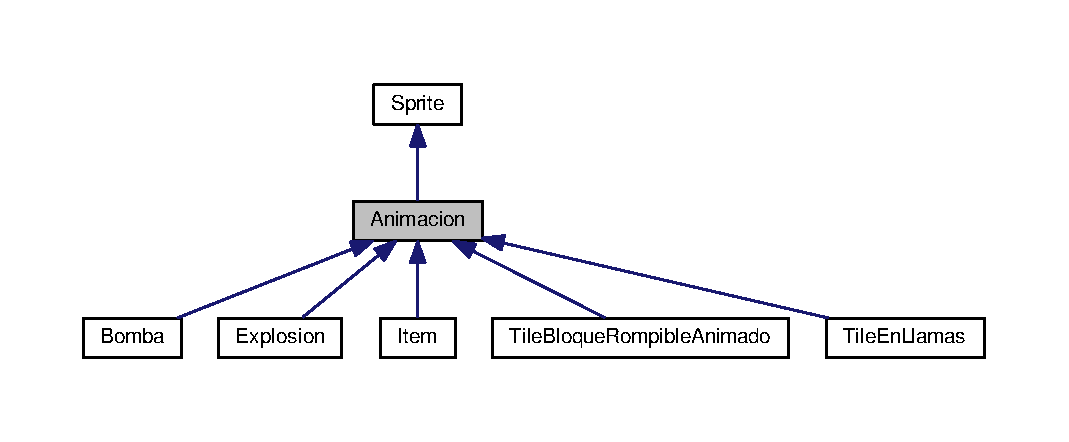
\includegraphics[width=350pt]{class_animacion__inherit__graph}
\end{center}
\end{figure}


Collaboration diagram for Animacion\+:\nopagebreak
\begin{figure}[H]
\begin{center}
\leavevmode
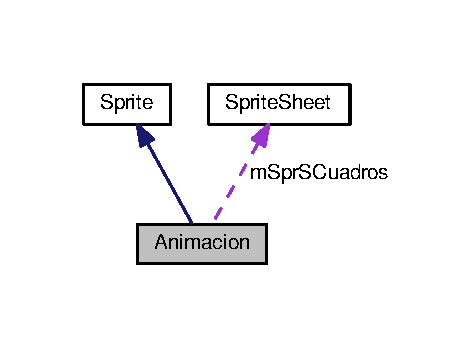
\includegraphics[width=227pt]{class_animacion__coll__graph}
\end{center}
\end{figure}
\subsection*{Public Member Functions}
\begin{DoxyCompactItemize}
\item 
{\bfseries Animacion} (\hyperlink{class_sprite_sheet}{Sprite\+Sheet} $\ast$sprite\+Sheet, string frames=N\+U\+LL, int x=0, int y=0, int delay\+Cambio\+Frame=2)\hypertarget{class_animacion_a42e4ac80569912ad50fcf23bce937908}{}\label{class_animacion_a42e4ac80569912ad50fcf23bce937908}

\item 
void {\bfseries update} (const Uint8 $\ast$keys=N\+U\+LL)\hypertarget{class_animacion_a9b52991c0710843e085326053b2ee568}{}\label{class_animacion_a9b52991c0710843e085326053b2ee568}

\item 
virtual void {\bfseries disable} ()\hypertarget{class_animacion_a02481ecab981d05dd0c50b46abb3f341}{}\label{class_animacion_a02481ecab981d05dd0c50b46abb3f341}

\item 
virtual void {\bfseries draw} (S\+D\+L\+\_\+\+Renderer $\ast$)\hypertarget{class_animacion_aee1eedfd331fb9cd1dbfdaf7550a866a}{}\label{class_animacion_aee1eedfd331fb9cd1dbfdaf7550a866a}

\item 
void {\bfseries move} (int nuevaX, int nuevaY) override\hypertarget{class_animacion_ae596bf2bc41b8a733fe5e2fae98b7850}{}\label{class_animacion_ae596bf2bc41b8a733fe5e2fae98b7850}

\item 
int {\bfseries get\+Cuadro} ()\hypertarget{class_animacion_aefb08950e8376addb0064df9fc39714a}{}\label{class_animacion_aefb08950e8376addb0064df9fc39714a}

\item 
void {\bfseries set\+Repeticiones} (int nuevo)\hypertarget{class_animacion_aa06923448345136fbd5d9d3b186168e9}{}\label{class_animacion_aa06923448345136fbd5d9d3b186168e9}

\item 
void {\bfseries set\+Cuadro\+Despues} (int nuevo)\hypertarget{class_animacion_aba6827dd1b9aa6ed1b8d92dd791d9195}{}\label{class_animacion_aba6827dd1b9aa6ed1b8d92dd791d9195}

\item 
void {\bfseries set\+Delay\+Cambio\+Frame} (int nuevo)\hypertarget{class_animacion_af9b3e2e5873daef7b1aa83d70d286596}{}\label{class_animacion_af9b3e2e5873daef7b1aa83d70d286596}

\item 
void {\bfseries set\+Cuadros\+Frames} (char $\ast$frames)\hypertarget{class_animacion_adfa64326dc3e8897449874cd89c409eb}{}\label{class_animacion_adfa64326dc3e8897449874cd89c409eb}

\end{DoxyCompactItemize}
\subsection*{Protected Attributes}
\begin{DoxyCompactItemize}
\item 
\hyperlink{class_sprite_sheet}{Sprite\+Sheet} $\ast$ {\bfseries m\+Spr\+S\+Cuadros} = nullptr\hypertarget{class_animacion_ad9a5ea56a2b3c88f8e5eec0d5c40653c}{}\label{class_animacion_ad9a5ea56a2b3c88f8e5eec0d5c40653c}

\item 
int {\bfseries m\+Repeticiones} = 0\hypertarget{class_animacion_adfac4172f4dea91d1c021744329c120a}{}\label{class_animacion_adfac4172f4dea91d1c021744329c120a}

\end{DoxyCompactItemize}


\subsection{Detailed Description}
Representa un \hyperlink{class_sprite}{Sprite} \char`\"{}\+Animado\char`\"{}

Es decir, que tiene una animacion.

La clase recive una \hyperlink{class_sprite}{Sprite} Sheet 

The documentation for this class was generated from the following files\+:\begin{DoxyCompactItemize}
\item 
src/engine/sprites/animacion/animacion.\+hpp\item 
src/engine/sprites/animacion/animacion.\+cpp\end{DoxyCompactItemize}

\hypertarget{class_animacion_desvanecer_out}{}\section{Animacion\+Desvanecer\+Out Class Reference}
\label{class_animacion_desvanecer_out}\index{Animacion\+Desvanecer\+Out@{Animacion\+Desvanecer\+Out}}


Inheritance diagram for Animacion\+Desvanecer\+Out\+:
\nopagebreak
\begin{figure}[H]
\begin{center}
\leavevmode
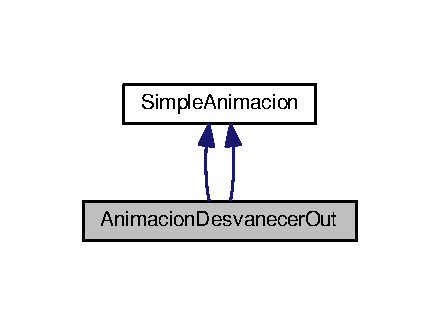
\includegraphics[width=211pt]{class_animacion_desvanecer_out__inherit__graph}
\end{center}
\end{figure}


Collaboration diagram for Animacion\+Desvanecer\+Out\+:
\nopagebreak
\begin{figure}[H]
\begin{center}
\leavevmode
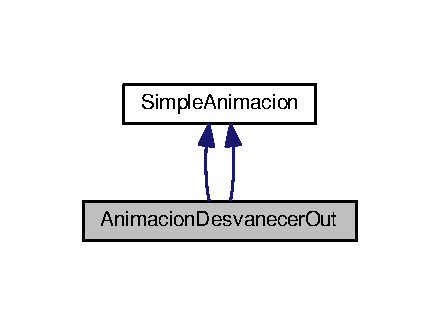
\includegraphics[width=211pt]{class_animacion_desvanecer_out__coll__graph}
\end{center}
\end{figure}
\subsection*{Public Member Functions}
\begin{DoxyCompactItemize}
\item 
{\bfseries Animacion\+Desvanecer\+Out} (S\+D\+L\+\_\+\+Texture $\ast$texture\+Out, int x, int y, int delay, int avance\+Speed)\hypertarget{class_animacion_desvanecer_out_af5d8f08dc57fd0c0493b83584f812ce3}{}\label{class_animacion_desvanecer_out_af5d8f08dc57fd0c0493b83584f812ce3}

\item 
void {\bfseries update} () override\hypertarget{class_animacion_desvanecer_out_ab775719c268e5a45580497df5688437c}{}\label{class_animacion_desvanecer_out_ab775719c268e5a45580497df5688437c}

\item 
void {\bfseries draw} (S\+D\+L\+\_\+\+Renderer $\ast$g\+Renderer) override\hypertarget{class_animacion_desvanecer_out_a9a4c2f15d0b3a9d723e4ed5d198e429b}{}\label{class_animacion_desvanecer_out_a9a4c2f15d0b3a9d723e4ed5d198e429b}

\item 
{\bfseries Animacion\+Desvanecer\+Out} (S\+D\+L\+\_\+\+Texture $\ast$texture\+Out, int x, int y, int delay, int avance\+Speed)\hypertarget{class_animacion_desvanecer_out_af5d8f08dc57fd0c0493b83584f812ce3}{}\label{class_animacion_desvanecer_out_af5d8f08dc57fd0c0493b83584f812ce3}

\item 
void {\bfseries update} () override\hypertarget{class_animacion_desvanecer_out_ab775719c268e5a45580497df5688437c}{}\label{class_animacion_desvanecer_out_ab775719c268e5a45580497df5688437c}

\item 
void {\bfseries draw} (S\+D\+L\+\_\+\+Renderer $\ast$g\+Renderer) override\hypertarget{class_animacion_desvanecer_out_a9a4c2f15d0b3a9d723e4ed5d198e429b}{}\label{class_animacion_desvanecer_out_a9a4c2f15d0b3a9d723e4ed5d198e429b}

\end{DoxyCompactItemize}
\subsection*{Additional Inherited Members}


The documentation for this class was generated from the following file\+:\begin{DoxyCompactItemize}
\item 
src/testsotrosjuegos/\+Othello/Animacion\+Desvanecer\+Out.\+hpp\end{DoxyCompactItemize}

\hypertarget{classrapidxml_1_1attribute__iterator}{}\section{rapidxml\+:\+:attribute\+\_\+iterator$<$ Ch $>$ Class Template Reference}
\label{classrapidxml_1_1attribute__iterator}\index{rapidxml\+::attribute\+\_\+iterator$<$ Ch $>$@{rapidxml\+::attribute\+\_\+iterator$<$ Ch $>$}}


Iterator of child attributes of \hyperlink{classrapidxml_1_1xml__node}{xml\+\_\+node}.  




{\ttfamily \#include $<$rapidxml\+\_\+iterators.\+hpp$>$}

\subsection*{Public Types}
\begin{DoxyCompactItemize}
\item 
typedef \hyperlink{classrapidxml_1_1xml__attribute}{xml\+\_\+attribute}$<$ Ch $>$ {\bfseries value\+\_\+type}\hypertarget{classrapidxml_1_1attribute__iterator_ad4280d358828ad9c3eb1a787decb162e}{}\label{classrapidxml_1_1attribute__iterator_ad4280d358828ad9c3eb1a787decb162e}

\item 
typedef \hyperlink{classrapidxml_1_1xml__attribute}{xml\+\_\+attribute}$<$ Ch $>$ \& {\bfseries reference}\hypertarget{classrapidxml_1_1attribute__iterator_a097343e44557de14de86b470d3f917d9}{}\label{classrapidxml_1_1attribute__iterator_a097343e44557de14de86b470d3f917d9}

\item 
typedef \hyperlink{classrapidxml_1_1xml__attribute}{xml\+\_\+attribute}$<$ Ch $>$ $\ast$ {\bfseries pointer}\hypertarget{classrapidxml_1_1attribute__iterator_a69acc2e60270d6a062c03c9cb1cf2aa7}{}\label{classrapidxml_1_1attribute__iterator_a69acc2e60270d6a062c03c9cb1cf2aa7}

\item 
typedef std\+::ptrdiff\+\_\+t {\bfseries difference\+\_\+type}\hypertarget{classrapidxml_1_1attribute__iterator_accfd6d8527d32b427496b42f71a2e37a}{}\label{classrapidxml_1_1attribute__iterator_accfd6d8527d32b427496b42f71a2e37a}

\item 
typedef std\+::bidirectional\+\_\+iterator\+\_\+tag {\bfseries iterator\+\_\+category}\hypertarget{classrapidxml_1_1attribute__iterator_a97ac5d8b98f5b03c68cc566f5ac0a9e0}{}\label{classrapidxml_1_1attribute__iterator_a97ac5d8b98f5b03c68cc566f5ac0a9e0}

\end{DoxyCompactItemize}
\subsection*{Public Member Functions}
\begin{DoxyCompactItemize}
\item 
{\bfseries attribute\+\_\+iterator} (\hyperlink{classrapidxml_1_1xml__node}{xml\+\_\+node}$<$ Ch $>$ $\ast$node)\hypertarget{classrapidxml_1_1attribute__iterator_a1109344dead88533ae4dd68cea5d9613}{}\label{classrapidxml_1_1attribute__iterator_a1109344dead88533ae4dd68cea5d9613}

\item 
\hyperlink{classrapidxml_1_1xml__attribute}{reference} {\bfseries operator$\ast$} () const \hypertarget{classrapidxml_1_1attribute__iterator_a5d8616bdd2d41119e2f342d77b4f56f9}{}\label{classrapidxml_1_1attribute__iterator_a5d8616bdd2d41119e2f342d77b4f56f9}

\item 
\hyperlink{classrapidxml_1_1xml__attribute}{pointer} {\bfseries operator-\/$>$} () const \hypertarget{classrapidxml_1_1attribute__iterator_a0975adffe3d178c0ac83652b9ab78791}{}\label{classrapidxml_1_1attribute__iterator_a0975adffe3d178c0ac83652b9ab78791}

\item 
\hyperlink{classrapidxml_1_1attribute__iterator}{attribute\+\_\+iterator} \& {\bfseries operator++} ()\hypertarget{classrapidxml_1_1attribute__iterator_afe7d15a4a1b228f97f1d4ebd4f3f6cca}{}\label{classrapidxml_1_1attribute__iterator_afe7d15a4a1b228f97f1d4ebd4f3f6cca}

\item 
\hyperlink{classrapidxml_1_1attribute__iterator}{attribute\+\_\+iterator} {\bfseries operator++} (int)\hypertarget{classrapidxml_1_1attribute__iterator_a82c8859b9eebd45caa3afc25b9e78c36}{}\label{classrapidxml_1_1attribute__iterator_a82c8859b9eebd45caa3afc25b9e78c36}

\item 
\hyperlink{classrapidxml_1_1attribute__iterator}{attribute\+\_\+iterator} \& {\bfseries operator-\/-\/} ()\hypertarget{classrapidxml_1_1attribute__iterator_af22f1ad3c11d3269b43b49e29b89d7d1}{}\label{classrapidxml_1_1attribute__iterator_af22f1ad3c11d3269b43b49e29b89d7d1}

\item 
\hyperlink{classrapidxml_1_1attribute__iterator}{attribute\+\_\+iterator} {\bfseries operator-\/-\/} (int)\hypertarget{classrapidxml_1_1attribute__iterator_af52a8562ab1b2c0391cdde79f55e4a6f}{}\label{classrapidxml_1_1attribute__iterator_af52a8562ab1b2c0391cdde79f55e4a6f}

\item 
bool {\bfseries operator==} (const \hyperlink{classrapidxml_1_1attribute__iterator}{attribute\+\_\+iterator}$<$ Ch $>$ \&rhs)\hypertarget{classrapidxml_1_1attribute__iterator_ab1dc8dd11d21e145a4e3f76d46aead0d}{}\label{classrapidxml_1_1attribute__iterator_ab1dc8dd11d21e145a4e3f76d46aead0d}

\item 
bool {\bfseries operator!=} (const \hyperlink{classrapidxml_1_1attribute__iterator}{attribute\+\_\+iterator}$<$ Ch $>$ \&rhs)\hypertarget{classrapidxml_1_1attribute__iterator_a39e8cf336c324521fd9c720abf280d88}{}\label{classrapidxml_1_1attribute__iterator_a39e8cf336c324521fd9c720abf280d88}

\end{DoxyCompactItemize}


\subsection{Detailed Description}
\subsubsection*{template$<$class Ch$>$\\*
class rapidxml\+::attribute\+\_\+iterator$<$ Ch $>$}

Iterator of child attributes of \hyperlink{classrapidxml_1_1xml__node}{xml\+\_\+node}. 

The documentation for this class was generated from the following file\+:\begin{DoxyCompactItemize}
\item 
src/engine/mapa/include/rapidxml/\hyperlink{rapidxml__iterators_8hpp}{rapidxml\+\_\+iterators.\+hpp}\end{DoxyCompactItemize}

\hypertarget{class_bitmap_font}{}\section{Bitmap\+Font Class Reference}
\label{class_bitmap_font}\index{Bitmap\+Font@{Bitmap\+Font}}
\subsection*{Public Member Functions}
\begin{DoxyCompactItemize}
\item 
{\bfseries Bitmap\+Font} (S\+D\+L\+\_\+\+Renderer $\ast$g\+Renderer, std\+::string ruta\+Imagen)\hypertarget{class_bitmap_font_a857c5fdf52ae5a93bc242ce98153b926}{}\label{class_bitmap_font_a857c5fdf52ae5a93bc242ce98153b926}

\item 
{\bfseries Bitmap\+Font} (S\+D\+L\+\_\+\+Renderer $\ast$g\+Renderer, std\+::string ruta\+Imagen)\hypertarget{class_bitmap_font_a857c5fdf52ae5a93bc242ce98153b926}{}\label{class_bitmap_font_a857c5fdf52ae5a93bc242ce98153b926}

\end{DoxyCompactItemize}
\subsection*{Friends}
\begin{DoxyCompactItemize}
\item 
class {\bfseries Bitmap\+Font\+Renderer}\hypertarget{class_bitmap_font_ada37f4b07dc117410a58a68940f82e46}{}\label{class_bitmap_font_ada37f4b07dc117410a58a68940f82e46}

\end{DoxyCompactItemize}


The documentation for this class was generated from the following file\+:\begin{DoxyCompactItemize}
\item 
src/testsotrosjuegos/\+Othello/Bitmap\+Font.\+hpp\end{DoxyCompactItemize}

\hypertarget{class_bitmap_font_renderer}{}\section{Bitmap\+Font\+Renderer Class Reference}
\label{class_bitmap_font_renderer}\index{Bitmap\+Font\+Renderer@{Bitmap\+Font\+Renderer}}
\subsection*{Public Member Functions}
\begin{DoxyCompactItemize}
\item 
{\bfseries Bitmap\+Font\+Renderer} (\hyperlink{class_bitmap_font}{Bitmap\+Font} $\ast$bitmap\+Font, int left, int top)\hypertarget{class_bitmap_font_renderer_a65e9126c5691f61c2d992a9ab996b79d}{}\label{class_bitmap_font_renderer_a65e9126c5691f61c2d992a9ab996b79d}

\item 
void {\bfseries set\+Bitmap\+Font} (\hyperlink{class_bitmap_font}{Bitmap\+Font} $\ast$nueva)\hypertarget{class_bitmap_font_renderer_a197dc934c3a667a0d0914044eafc8c79}{}\label{class_bitmap_font_renderer_a197dc934c3a667a0d0914044eafc8c79}

\item 
void {\bfseries set\+Text} (std\+::string nueva)\hypertarget{class_bitmap_font_renderer_a8d0a1192a86938db8d62f6c0e2ba337d}{}\label{class_bitmap_font_renderer_a8d0a1192a86938db8d62f6c0e2ba337d}

\item 
void {\bfseries set\+Right} (int right)\hypertarget{class_bitmap_font_renderer_a3dee9252829f28f6feacb2d1a44afabb}{}\label{class_bitmap_font_renderer_a3dee9252829f28f6feacb2d1a44afabb}

\item 
void {\bfseries set\+Bottom} (int bottom)\hypertarget{class_bitmap_font_renderer_a309059d65d1b9bc39aa0ff7106f6953f}{}\label{class_bitmap_font_renderer_a309059d65d1b9bc39aa0ff7106f6953f}

\item 
void {\bfseries set\+Top} (int top)\hypertarget{class_bitmap_font_renderer_a86a56db51e9b5f0c88b867231668ca00}{}\label{class_bitmap_font_renderer_a86a56db51e9b5f0c88b867231668ca00}

\item 
void {\bfseries set\+Left} (int left)\hypertarget{class_bitmap_font_renderer_a9894805617288d3f5b652dcc30ab5f45}{}\label{class_bitmap_font_renderer_a9894805617288d3f5b652dcc30ab5f45}

\item 
void {\bfseries draw} (S\+D\+L\+\_\+\+Renderer $\ast$g\+Renderer)\hypertarget{class_bitmap_font_renderer_a5b6268da07617eb4af60dd5c29e3c0ba}{}\label{class_bitmap_font_renderer_a5b6268da07617eb4af60dd5c29e3c0ba}

\item 
int {\bfseries get\+Left} ()\hypertarget{class_bitmap_font_renderer_a9a46c5f2dc06587090df845a1a025cfc}{}\label{class_bitmap_font_renderer_a9a46c5f2dc06587090df845a1a025cfc}

\item 
int {\bfseries get\+Top} ()\hypertarget{class_bitmap_font_renderer_aa4944663fb8a76418ebbbf90293b7bf0}{}\label{class_bitmap_font_renderer_aa4944663fb8a76418ebbbf90293b7bf0}

\item 
int {\bfseries get\+Height} ()\hypertarget{class_bitmap_font_renderer_a1f3af2d5ee811b92b0974d667bea5f02}{}\label{class_bitmap_font_renderer_a1f3af2d5ee811b92b0974d667bea5f02}

\item 
void {\bfseries draw} (S\+D\+L\+\_\+\+Renderer $\ast$p\+Renderer, int x, int y)\hypertarget{class_bitmap_font_renderer_a1d64e6aeb450d94e7f32f1634a4c9d5e}{}\label{class_bitmap_font_renderer_a1d64e6aeb450d94e7f32f1634a4c9d5e}

\item 
{\bfseries Bitmap\+Font\+Renderer} (\hyperlink{class_bitmap_font}{Bitmap\+Font} $\ast$bitmap\+Font, int left, int top)\hypertarget{class_bitmap_font_renderer_a65e9126c5691f61c2d992a9ab996b79d}{}\label{class_bitmap_font_renderer_a65e9126c5691f61c2d992a9ab996b79d}

\item 
void {\bfseries set\+Bitmap\+Font} (\hyperlink{class_bitmap_font}{Bitmap\+Font} $\ast$nueva)\hypertarget{class_bitmap_font_renderer_a197dc934c3a667a0d0914044eafc8c79}{}\label{class_bitmap_font_renderer_a197dc934c3a667a0d0914044eafc8c79}

\item 
void {\bfseries set\+Text} (std\+::string nueva)\hypertarget{class_bitmap_font_renderer_a8d0a1192a86938db8d62f6c0e2ba337d}{}\label{class_bitmap_font_renderer_a8d0a1192a86938db8d62f6c0e2ba337d}

\item 
void {\bfseries set\+Right} (int right)\hypertarget{class_bitmap_font_renderer_a3dee9252829f28f6feacb2d1a44afabb}{}\label{class_bitmap_font_renderer_a3dee9252829f28f6feacb2d1a44afabb}

\item 
void {\bfseries set\+Bottom} (int bottom)\hypertarget{class_bitmap_font_renderer_a309059d65d1b9bc39aa0ff7106f6953f}{}\label{class_bitmap_font_renderer_a309059d65d1b9bc39aa0ff7106f6953f}

\item 
void {\bfseries set\+Top} (int top)\hypertarget{class_bitmap_font_renderer_a86a56db51e9b5f0c88b867231668ca00}{}\label{class_bitmap_font_renderer_a86a56db51e9b5f0c88b867231668ca00}

\item 
void {\bfseries set\+Left} (int left)\hypertarget{class_bitmap_font_renderer_a9894805617288d3f5b652dcc30ab5f45}{}\label{class_bitmap_font_renderer_a9894805617288d3f5b652dcc30ab5f45}

\item 
void {\bfseries draw} (S\+D\+L\+\_\+\+Renderer $\ast$g\+Renderer)\hypertarget{class_bitmap_font_renderer_a5b6268da07617eb4af60dd5c29e3c0ba}{}\label{class_bitmap_font_renderer_a5b6268da07617eb4af60dd5c29e3c0ba}

\item 
int {\bfseries get\+Left} ()\hypertarget{class_bitmap_font_renderer_a9a46c5f2dc06587090df845a1a025cfc}{}\label{class_bitmap_font_renderer_a9a46c5f2dc06587090df845a1a025cfc}

\item 
int {\bfseries get\+Top} ()\hypertarget{class_bitmap_font_renderer_aa4944663fb8a76418ebbbf90293b7bf0}{}\label{class_bitmap_font_renderer_aa4944663fb8a76418ebbbf90293b7bf0}

\item 
int {\bfseries get\+Height} ()\hypertarget{class_bitmap_font_renderer_a1f3af2d5ee811b92b0974d667bea5f02}{}\label{class_bitmap_font_renderer_a1f3af2d5ee811b92b0974d667bea5f02}

\item 
void {\bfseries draw} (S\+D\+L\+\_\+\+Renderer $\ast$p\+Renderer, int x, int y)\hypertarget{class_bitmap_font_renderer_a1d64e6aeb450d94e7f32f1634a4c9d5e}{}\label{class_bitmap_font_renderer_a1d64e6aeb450d94e7f32f1634a4c9d5e}

\end{DoxyCompactItemize}


The documentation for this class was generated from the following file\+:\begin{DoxyCompactItemize}
\item 
src/testsotrosjuegos/\+Othello/Bitmap\+Font.\+hpp\end{DoxyCompactItemize}

\hypertarget{class_bomba}{}\section{Bomba Class Reference}
\label{class_bomba}\index{Bomba@{Bomba}}


Inheritance diagram for Bomba\+:\nopagebreak
\begin{figure}[H]
\begin{center}
\leavevmode
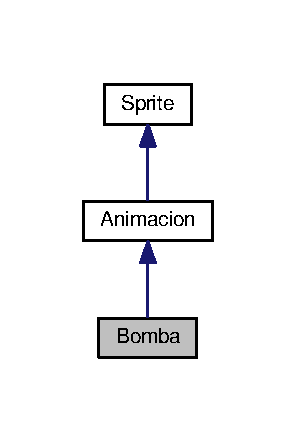
\includegraphics[width=142pt]{class_bomba__inherit__graph}
\end{center}
\end{figure}


Collaboration diagram for Bomba\+:\nopagebreak
\begin{figure}[H]
\begin{center}
\leavevmode
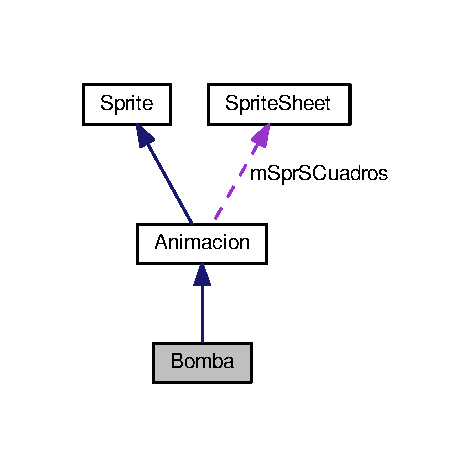
\includegraphics[width=227pt]{class_bomba__coll__graph}
\end{center}
\end{figure}
\subsection*{Public Member Functions}
\begin{DoxyCompactItemize}
\item 
{\bfseries Bomba} (S\+D\+L\+\_\+\+Renderer $\ast$g\+Renderer, \hyperlink{class_player}{Player} $\ast$propietario)\hypertarget{class_bomba_a1e5390984a730fd046847dc8b5334eb5}{}\label{class_bomba_a1e5390984a730fd046847dc8b5334eb5}

\item 
\hyperlink{class_player}{Player} $\ast$ {\bfseries get\+Player\+Propietario} ()\hypertarget{class_bomba_a236e2f12b525c781c1bb518e9e2fa274}{}\label{class_bomba_a236e2f12b525c781c1bb518e9e2fa274}

\item 
void {\bfseries set\+Repeticion} (int nuevo)\hypertarget{class_bomba_a46fe0c87eab4a86edfb0fdec355275ac}{}\label{class_bomba_a46fe0c87eab4a86edfb0fdec355275ac}

\end{DoxyCompactItemize}
\subsection*{Additional Inherited Members}


The documentation for this class was generated from the following file\+:\begin{DoxyCompactItemize}
\item 
src/personajes/bomba.\+hpp\end{DoxyCompactItemize}

\hypertarget{class_boton_component}{}\section{Boton\+Component$<$ T $>$ Class Template Reference}
\label{class_boton_component}\index{Boton\+Component$<$ T $>$@{Boton\+Component$<$ T $>$}}


Inheritance diagram for Boton\+Component$<$ T $>$\+:\nopagebreak
\begin{figure}[H]
\begin{center}
\leavevmode
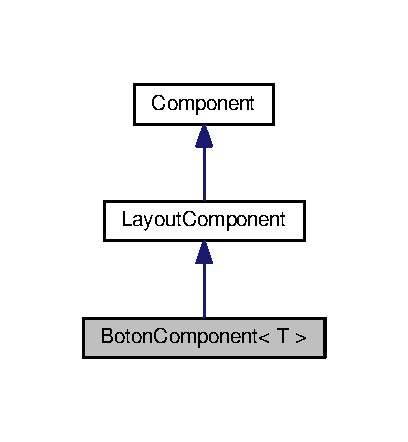
\includegraphics[width=196pt]{class_boton_component__inherit__graph}
\end{center}
\end{figure}


Collaboration diagram for Boton\+Component$<$ T $>$\+:\nopagebreak
\begin{figure}[H]
\begin{center}
\leavevmode
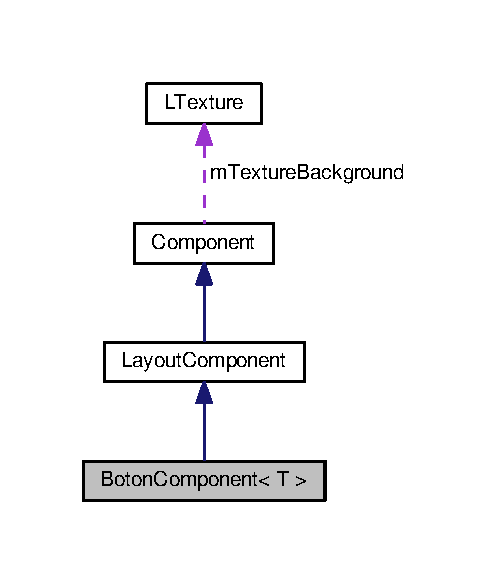
\includegraphics[width=235pt]{class_boton_component__coll__graph}
\end{center}
\end{figure}
\subsection*{Public Types}
\begin{DoxyCompactItemize}
\item 
enum {\bfseries Estado} \{ {\bfseries N\+O\+R\+M\+AL}, 
{\bfseries R\+E\+S\+A\+L\+T\+A\+DO}, 
{\bfseries P\+R\+E\+S\+I\+O\+N\+A\+DO}, 
{\bfseries \+\_\+\+E\+S\+T\+A\+D\+OS}
 \}\hypertarget{class_boton_component_a15cc75d9064e182d8acb9240831e873d}{}\label{class_boton_component_a15cc75d9064e182d8acb9240831e873d}

\end{DoxyCompactItemize}
\subsection*{Public Member Functions}
\begin{DoxyCompactItemize}
\item 
{\bfseries Boton\+Component} (\hyperlink{class_l_texture}{L\+Texture} $\ast$grilla, T $\ast$parent=N\+U\+LL)\hypertarget{class_boton_component_a1b246f7b92a8a69a9e6045cfde653e5a}{}\label{class_boton_component_a1b246f7b92a8a69a9e6045cfde653e5a}

\item 
void \hyperlink{class_boton_component_adacc77cd1e8f7d40a2f30b4b7b61899c}{pack} (S\+D\+L\+\_\+\+Renderer $\ast$g\+Renderer) override
\item 
void {\bfseries procesar\+Evento} (S\+D\+L\+\_\+\+Event $\ast$evento)\hypertarget{class_boton_component_adb8885d42fb91509b5d13a535b91948f}{}\label{class_boton_component_adb8885d42fb91509b5d13a535b91948f}

\item 
void {\bfseries bind\+Accion} (void(T\+::$\ast$p\+Accion)(void))\hypertarget{class_boton_component_af57c381f836ca99809f70df6e270ccc8}{}\label{class_boton_component_af57c381f836ca99809f70df6e270ccc8}

\item 
void {\bfseries bind\+Accion} (void(T\+::$\ast$p\+Accion)(\hyperlink{class_boton_component}{Boton\+Component}$<$ T $>$ $\ast$))\hypertarget{class_boton_component_ae98007d5eae6e6bfb180544dbc533236}{}\label{class_boton_component_ae98007d5eae6e6bfb180544dbc533236}

\item 
void \hyperlink{class_boton_component_a73c8c3014be82c952cd8d0e08beffcc5}{draw} (S\+D\+L\+\_\+\+Renderer $\ast$g\+Renderer) override
\item 
bool {\bfseries get\+Visible} ()\hypertarget{class_boton_component_a3204169da97382286dd8b96eaec9e7a5}{}\label{class_boton_component_a3204169da97382286dd8b96eaec9e7a5}

\item 
bool {\bfseries get\+Enable} ()\hypertarget{class_boton_component_a60bdb5f4b30fa92ca442cac257a05243}{}\label{class_boton_component_a60bdb5f4b30fa92ca442cac257a05243}

\item 
bool {\bfseries esta\+Presionado} ()\hypertarget{class_boton_component_a3b5ff7608fa03e2e0c56f46a08cb3e44}{}\label{class_boton_component_a3b5ff7608fa03e2e0c56f46a08cb3e44}

\item 
void {\bfseries set\+Visible} (bool nuevo)\hypertarget{class_boton_component_aa8fcb117c496db9d68168aaf5149d036}{}\label{class_boton_component_aa8fcb117c496db9d68168aaf5149d036}

\item 
void {\bfseries set\+Enable} (bool nuevo)\hypertarget{class_boton_component_a545222f3de978fa9d91e84df09d53bec}{}\label{class_boton_component_a545222f3de978fa9d91e84df09d53bec}

\item 
void {\bfseries set\+Estado} (Estado nuevo)\hypertarget{class_boton_component_a864923b6ab72aa69660c77ff8485156f}{}\label{class_boton_component_a864923b6ab72aa69660c77ff8485156f}

\item 
void {\bfseries set\+Id} (int nuevo)\hypertarget{class_boton_component_aac900d1f2371e566a7ce79f508fedd47}{}\label{class_boton_component_aac900d1f2371e566a7ce79f508fedd47}

\item 
int {\bfseries get\+Id} ()\hypertarget{class_boton_component_a2b712691635f375c508f1a000aba5927}{}\label{class_boton_component_a2b712691635f375c508f1a000aba5927}

\end{DoxyCompactItemize}
\subsection*{Additional Inherited Members}


\subsection{Member Function Documentation}
\index{Boton\+Component@{Boton\+Component}!draw@{draw}}
\index{draw@{draw}!Boton\+Component@{Boton\+Component}}
\subsubsection[{\texorpdfstring{draw(\+S\+D\+L\+\_\+\+Renderer $\ast$g\+Renderer) override}{draw(SDL_Renderer *gRenderer) override}}]{\setlength{\rightskip}{0pt plus 5cm}template$<$typename T$>$ void {\bf Boton\+Component}$<$ T $>$\+::draw (
\begin{DoxyParamCaption}
\item[{S\+D\+L\+\_\+\+Renderer $\ast$}]{g\+Renderer}
\end{DoxyParamCaption}
)\hspace{0.3cm}{\ttfamily [inline]}, {\ttfamily [override]}, {\ttfamily [virtual]}}\hypertarget{class_boton_component_a73c8c3014be82c952cd8d0e08beffcc5}{}\label{class_boton_component_a73c8c3014be82c952cd8d0e08beffcc5}
Dibuja el componente 
\begin{DoxyParams}{Parameters}
{\em g\+Renderer} & \\
\hline
\end{DoxyParams}


Reimplemented from \hyperlink{class_component_ab1ea202c9ef8933d15956b96cfe281a1}{Component}.

\index{Boton\+Component@{Boton\+Component}!pack@{pack}}
\index{pack@{pack}!Boton\+Component@{Boton\+Component}}
\subsubsection[{\texorpdfstring{pack(\+S\+D\+L\+\_\+\+Renderer $\ast$g\+Renderer) override}{pack(SDL_Renderer *gRenderer) override}}]{\setlength{\rightskip}{0pt plus 5cm}template$<$typename T$>$ void {\bf Boton\+Component}$<$ T $>$\+::pack (
\begin{DoxyParamCaption}
\item[{S\+D\+L\+\_\+\+Renderer $\ast$}]{g\+Renderer}
\end{DoxyParamCaption}
)\hspace{0.3cm}{\ttfamily [inline]}, {\ttfamily [override]}, {\ttfamily [virtual]}}\hypertarget{class_boton_component_adacc77cd1e8f7d40a2f30b4b7b61899c}{}\label{class_boton_component_adacc77cd1e8f7d40a2f30b4b7b61899c}
Se encarga de crear las texturas del componente asi como otras acciones asociadas con el renderer Notar que despues de esta funcion se debe llamar a calculate\+Rect, es decir, realizar una nueva calculacion del rectangulo de dibujo del componente 
\begin{DoxyParams}{Parameters}
{\em g\+Renderer} & Render de la pantalla \\
\hline
\end{DoxyParams}


Implements \hyperlink{class_component_aa471f2c3a24525f584ed19cf25222e70}{Component}.



The documentation for this class was generated from the following file\+:\begin{DoxyCompactItemize}
\item 
src/engine/layout/\+Componentes/Boton\+Component.\+hpp\end{DoxyCompactItemize}

\hypertarget{class_c_font}{}\section{C\+Font Class Reference}
\label{class_c_font}\index{C\+Font@{C\+Font}}


{\ttfamily \#include $<$C\+Font.\+hpp$>$}

\subsection*{Public Member Functions}
\begin{DoxyCompactItemize}
\item 
\hyperlink{class_c_font_a3f49893acc711805888c11aa8e931666}{C\+Font} ()
\item 
bool {\bfseries load\+Font} (string path\+Font, int size)\hypertarget{class_c_font_a85d82f9d94ccc313de3afc6a01798a0e}{}\label{class_c_font_a85d82f9d94ccc313de3afc6a01798a0e}

\item 
\hyperlink{class_l_texture}{L\+Texture} $\ast$ {\bfseries create\+Texture\+From\+Text} (S\+D\+L\+\_\+\+Renderer $\ast$g\+Renderer, string texto)\hypertarget{class_c_font_ab4d6760a2c774a562fc694145c3705e7}{}\label{class_c_font_ab4d6760a2c774a562fc694145c3705e7}

\item 
void {\bfseries set\+Text\+Color} (S\+D\+L\+\_\+\+Color color)\hypertarget{class_c_font_ae793580013df4543d4f3c51c96676152}{}\label{class_c_font_ae793580013df4543d4f3c51c96676152}

\item 
std\+::string {\bfseries get\+Path\+Font} ()\hypertarget{class_c_font_afde5392ae1f78e95537dc09078397392}{}\label{class_c_font_afde5392ae1f78e95537dc09078397392}

\end{DoxyCompactItemize}


\subsection{Detailed Description}
Escribe un texto en pantalla usando una imagen que contiene las letras en un orden 

\subsection{Constructor \& Destructor Documentation}
\index{C\+Font@{C\+Font}!C\+Font@{C\+Font}}
\index{C\+Font@{C\+Font}!C\+Font@{C\+Font}}
\subsubsection[{\texorpdfstring{C\+Font()}{CFont()}}]{\setlength{\rightskip}{0pt plus 5cm}C\+Font\+::\+C\+Font (
\begin{DoxyParamCaption}
{}
\end{DoxyParamCaption}
)}\hypertarget{class_c_font_a3f49893acc711805888c11aa8e931666}{}\label{class_c_font_a3f49893acc711805888c11aa8e931666}
Inicia las variables 

The documentation for this class was generated from the following files\+:\begin{DoxyCompactItemize}
\item 
src/engine/util/C\+Font.\+hpp\item 
src/engine/util/C\+Font.\+cpp\end{DoxyCompactItemize}

\hypertarget{class_component}{}\section{Component Class Reference}
\label{class_component}\index{Component@{Component}}


Inheritance diagram for Component\+:
\nopagebreak
\begin{figure}[H]
\begin{center}
\leavevmode
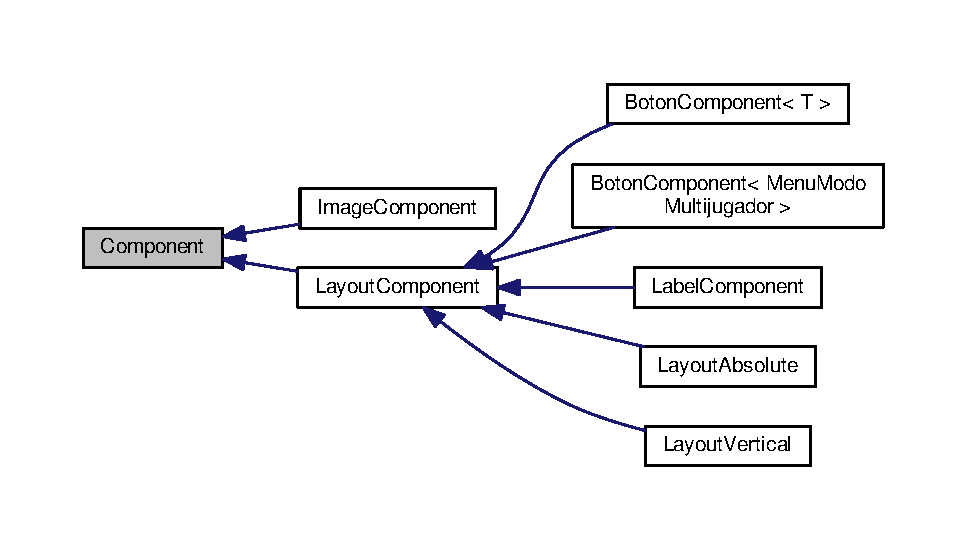
\includegraphics[width=350pt]{class_component__inherit__graph}
\end{center}
\end{figure}


Collaboration diagram for Component\+:\nopagebreak
\begin{figure}[H]
\begin{center}
\leavevmode
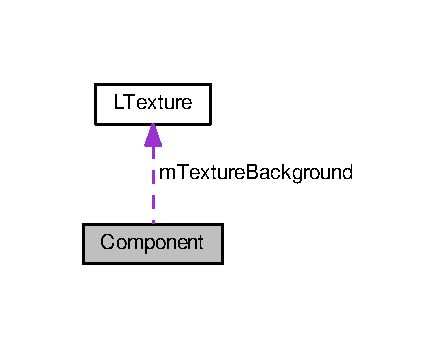
\includegraphics[width=211pt]{class_component__coll__graph}
\end{center}
\end{figure}
\subsection*{Public Member Functions}
\begin{DoxyCompactItemize}
\item 
\hyperlink{class_component_a8775db6d1a2c1afc2e77cd3c8f39da6f}{Component} ()
\item 
void {\bfseries set\+Layout\+Param} (std\+::string name\+Param, std\+::string value\+Param)\hypertarget{class_component_ae36d03537d53b88e2b4776250787f842}{}\label{class_component_ae36d03537d53b88e2b4776250787f842}

\item 
void {\bfseries add\+Layout\+Param} (std\+::string name\+Param, std\+::string value\+Param)\hypertarget{class_component_ae79cb654e6be297577f35c599d34254c}{}\label{class_component_ae79cb654e6be297577f35c599d34254c}

\item 
std\+::string {\bfseries get\+Layout\+Param} (std\+::string name\+Param)\hypertarget{class_component_a2c1f1bf9132f6784d46150b90fe89500}{}\label{class_component_a2c1f1bf9132f6784d46150b90fe89500}

\item 
void \hyperlink{class_component_a354add2c6de9a08357fbfece7fe50ac5}{set\+Background\+Texture} (\hyperlink{class_l_texture}{L\+Texture} $\ast$l\+Texture, bool delete\+Anterior=true)
\item 
void \hyperlink{class_component_a1440d7c2b2c4bfd8310931b54e8f4e61}{set\+Disabled} (bool nuevo)
\item 
virtual bool \hyperlink{class_component_aedd9acaa31b5c50a8cf233014b85c0cc}{is\+Disabled} ()
\item 
int {\bfseries get\+Internal\+Width} ()\hypertarget{class_component_a27900513de0e1cd920ffb0788f144bc9}{}\label{class_component_a27900513de0e1cd920ffb0788f144bc9}

\item 
int {\bfseries get\+Internal\+Height} ()\hypertarget{class_component_a74576e7c5591fe7adc74a18c9fa752e4}{}\label{class_component_a74576e7c5591fe7adc74a18c9fa752e4}

\item 
virtual void \hyperlink{class_component_aa471f2c3a24525f584ed19cf25222e70}{pack} (S\+D\+L\+\_\+\+Renderer $\ast$g\+Renderer)=0
\item 
virtual void {\bfseries set\+Rect\+Dibujo} (S\+D\+L\+\_\+\+Rect \&rect)\hypertarget{class_component_a06933061417ef2fec8588e731802c76b}{}\label{class_component_a06933061417ef2fec8588e731802c76b}

\item 
void \hyperlink{class_component_a0df4f4d3aaac6083dc6fe7c9ec1e9435}{set\+Background\+Color} (S\+D\+L\+\_\+\+Color color)
\item 
virtual void \hyperlink{class_component_ab1ea202c9ef8933d15956b96cfe281a1}{draw} (S\+D\+L\+\_\+\+Renderer $\ast$g\+Renderer)
\item 
void {\bfseries set\+Background\+Texture} (S\+D\+L\+\_\+\+Renderer $\ast$p\+Renderer, std\+::string ruta, bool tiene\+Color\+Clave)\hypertarget{class_component_af5266ecac7180548cf2282377ca70752}{}\label{class_component_af5266ecac7180548cf2282377ca70752}

\end{DoxyCompactItemize}
\subsection*{Protected Attributes}
\begin{DoxyCompactItemize}
\item 
std\+::unordered\+\_\+map$<$ std\+::string, std\+::string $>$ {\bfseries m\+Layout\+Params}\hypertarget{class_component_aa57d48b13ce8d6d0cbad5d2df25855e9}{}\label{class_component_aa57d48b13ce8d6d0cbad5d2df25855e9}

\item 
\hyperlink{class_l_texture}{L\+Texture} $\ast$ {\bfseries m\+Texture\+Background}\hypertarget{class_component_a1146357f9295249aa37d441a1055cfcb}{}\label{class_component_a1146357f9295249aa37d441a1055cfcb}

\item 
bool {\bfseries m\+Disabled}\hypertarget{class_component_a31f905a630a60deb299a3c598de040eb}{}\label{class_component_a31f905a630a60deb299a3c598de040eb}

\item 
S\+D\+L\+\_\+\+Rect {\bfseries m\+Internal\+Rect}\hypertarget{class_component_ab29a46348bb17e085bc2d204b5e9809f}{}\label{class_component_ab29a46348bb17e085bc2d204b5e9809f}

\item 
S\+D\+L\+\_\+\+Color {\bfseries m\+Background\+Color}\hypertarget{class_component_a0eeef3ba6bce588f0908cbaa34113c42}{}\label{class_component_a0eeef3ba6bce588f0908cbaa34113c42}

\item 
bool {\bfseries m\+Establecido\+Color\+Fondo}\hypertarget{class_component_a17b8acdefc67020f12ade56dedb070ce}{}\label{class_component_a17b8acdefc67020f12ade56dedb070ce}

\item 
S\+D\+L\+\_\+\+Rect {\bfseries m\+Draw\+Rect}\hypertarget{class_component_a6182ec25ba26a0d1616662e547ed4afe}{}\label{class_component_a6182ec25ba26a0d1616662e547ed4afe}

\end{DoxyCompactItemize}


\subsection{Constructor \& Destructor Documentation}
\index{Component@{Component}!Component@{Component}}
\index{Component@{Component}!Component@{Component}}
\subsubsection[{\texorpdfstring{Component()}{Component()}}]{\setlength{\rightskip}{0pt plus 5cm}Component\+::\+Component (
\begin{DoxyParamCaption}
{}
\end{DoxyParamCaption}
)\hspace{0.3cm}{\ttfamily [inline]}}\hypertarget{class_component_a8775db6d1a2c1afc2e77cd3c8f39da6f}{}\label{class_component_a8775db6d1a2c1afc2e77cd3c8f39da6f}
Inicializa el componente \begin{DoxyReturn}{Returns}

\end{DoxyReturn}


\subsection{Member Function Documentation}
\index{Component@{Component}!draw@{draw}}
\index{draw@{draw}!Component@{Component}}
\subsubsection[{\texorpdfstring{draw(\+S\+D\+L\+\_\+\+Renderer $\ast$g\+Renderer)}{draw(SDL_Renderer *gRenderer)}}]{\setlength{\rightskip}{0pt plus 5cm}virtual void Component\+::draw (
\begin{DoxyParamCaption}
\item[{S\+D\+L\+\_\+\+Renderer $\ast$}]{g\+Renderer}
\end{DoxyParamCaption}
)\hspace{0.3cm}{\ttfamily [inline]}, {\ttfamily [virtual]}}\hypertarget{class_component_ab1ea202c9ef8933d15956b96cfe281a1}{}\label{class_component_ab1ea202c9ef8933d15956b96cfe281a1}
Dibuja el componente 
\begin{DoxyParams}{Parameters}
{\em g\+Renderer} & \\
\hline
\end{DoxyParams}


Reimplemented in \hyperlink{class_boton_component_a73c8c3014be82c952cd8d0e08beffcc5}{Boton\+Component$<$ T $>$}, \hyperlink{class_boton_component_a73c8c3014be82c952cd8d0e08beffcc5}{Boton\+Component$<$ Menu\+Modo\+Multijugador $>$}, \hyperlink{class_label_component_a9637b7af88eb351108ef490f175b39a9}{Label\+Component}, and \hyperlink{class_layout_component_a0ee8a3146a3258a9886472b86cf34a16}{Layout\+Component}.

\index{Component@{Component}!is\+Disabled@{is\+Disabled}}
\index{is\+Disabled@{is\+Disabled}!Component@{Component}}
\subsubsection[{\texorpdfstring{is\+Disabled()}{isDisabled()}}]{\setlength{\rightskip}{0pt plus 5cm}virtual bool Component\+::is\+Disabled (
\begin{DoxyParamCaption}
{}
\end{DoxyParamCaption}
)\hspace{0.3cm}{\ttfamily [inline]}, {\ttfamily [virtual]}}\hypertarget{class_component_aedd9acaa31b5c50a8cf233014b85c0cc}{}\label{class_component_aedd9acaa31b5c50a8cf233014b85c0cc}
Retorna el estado de la variable m\+Disabled. \begin{DoxyReturn}{Returns}

\end{DoxyReturn}


Reimplemented in \hyperlink{class_layout_absolute_aba1ab3840e566a65bdecb4ba8a249eac}{Layout\+Absolute}, and \hyperlink{class_layout_vertical_a90f1b16b40a8765bb59d536b667e13e4}{Layout\+Vertical}.

\index{Component@{Component}!pack@{pack}}
\index{pack@{pack}!Component@{Component}}
\subsubsection[{\texorpdfstring{pack(\+S\+D\+L\+\_\+\+Renderer $\ast$g\+Renderer)=0}{pack(SDL_Renderer *gRenderer)=0}}]{\setlength{\rightskip}{0pt plus 5cm}virtual void Component\+::pack (
\begin{DoxyParamCaption}
\item[{S\+D\+L\+\_\+\+Renderer $\ast$}]{g\+Renderer}
\end{DoxyParamCaption}
)\hspace{0.3cm}{\ttfamily [pure virtual]}}\hypertarget{class_component_aa471f2c3a24525f584ed19cf25222e70}{}\label{class_component_aa471f2c3a24525f584ed19cf25222e70}
Se encarga de crear las texturas del componente asi como otras acciones asociadas con el renderer Notar que despues de esta funcion se debe llamar a calculate\+Rect, es decir, realizar una nueva calculacion del rectangulo de dibujo del componente 
\begin{DoxyParams}{Parameters}
{\em g\+Renderer} & Render de la pantalla \\
\hline
\end{DoxyParams}


Implemented in \hyperlink{class_layout_absolute_a9807517212f0015c0a67399a35f1ff36}{Layout\+Absolute}, \hyperlink{class_layout_vertical_a02eea5b9dd8197100d964d0e6f33e208}{Layout\+Vertical}, \hyperlink{class_boton_component_adacc77cd1e8f7d40a2f30b4b7b61899c}{Boton\+Component$<$ T $>$}, \hyperlink{class_boton_component_adacc77cd1e8f7d40a2f30b4b7b61899c}{Boton\+Component$<$ Menu\+Modo\+Multijugador $>$}, \hyperlink{class_label_component_a9979a17ac60f351d9850e0d670d8ab0e}{Label\+Component}, and \hyperlink{class_image_component_a538cae4b9b1f723fa6cb21038387a0f6}{Image\+Component}.

\index{Component@{Component}!set\+Background\+Color@{set\+Background\+Color}}
\index{set\+Background\+Color@{set\+Background\+Color}!Component@{Component}}
\subsubsection[{\texorpdfstring{set\+Background\+Color(\+S\+D\+L\+\_\+\+Color color)}{setBackgroundColor(SDL_Color color)}}]{\setlength{\rightskip}{0pt plus 5cm}void Component\+::set\+Background\+Color (
\begin{DoxyParamCaption}
\item[{S\+D\+L\+\_\+\+Color}]{color}
\end{DoxyParamCaption}
)\hspace{0.3cm}{\ttfamily [inline]}}\hypertarget{class_component_a0df4f4d3aaac6083dc6fe7c9ec1e9435}{}\label{class_component_a0df4f4d3aaac6083dc6fe7c9ec1e9435}
Establece un color de fondo para el componente 
\begin{DoxyParams}{Parameters}
{\em color} & \\
\hline
\end{DoxyParams}
\begin{Desc}
\item[Examples\+: ]\par
\hyperlink{_2home_2manuggz_2_documents_2_projects_2_bomberman_2src_2engine_2interfaces_2_menu_list_label_8hpp-example}{/home/manuggz/\+Documents/\+Projects/\+Bomberman/src/engine/interfaces/\+Menu\+List\+Label.\+hpp}.\end{Desc}
\index{Component@{Component}!set\+Background\+Texture@{set\+Background\+Texture}}
\index{set\+Background\+Texture@{set\+Background\+Texture}!Component@{Component}}
\subsubsection[{\texorpdfstring{set\+Background\+Texture(\+L\+Texture $\ast$l\+Texture, bool delete\+Anterior=true)}{setBackgroundTexture(LTexture *lTexture, bool deleteAnterior=true)}}]{\setlength{\rightskip}{0pt plus 5cm}void Component\+::set\+Background\+Texture (
\begin{DoxyParamCaption}
\item[{{\bf L\+Texture} $\ast$}]{l\+Texture, }
\item[{bool}]{delete\+Anterior = {\ttfamily true}}
\end{DoxyParamCaption}
)\hspace{0.3cm}{\ttfamily [inline]}}\hypertarget{class_component_a354add2c6de9a08357fbfece7fe50ac5}{}\label{class_component_a354add2c6de9a08357fbfece7fe50ac5}
Establece la textura a dibujar en el fondo del componente 
\begin{DoxyParams}{Parameters}
{\em l\+Texture} & \\
\hline
\end{DoxyParams}
\index{Component@{Component}!set\+Disabled@{set\+Disabled}}
\index{set\+Disabled@{set\+Disabled}!Component@{Component}}
\subsubsection[{\texorpdfstring{set\+Disabled(bool nuevo)}{setDisabled(bool nuevo)}}]{\setlength{\rightskip}{0pt plus 5cm}void Component\+::set\+Disabled (
\begin{DoxyParamCaption}
\item[{bool}]{nuevo}
\end{DoxyParamCaption}
)\hspace{0.3cm}{\ttfamily [inline]}}\hypertarget{class_component_a1440d7c2b2c4bfd8310931b54e8f4e61}{}\label{class_component_a1440d7c2b2c4bfd8310931b54e8f4e61}
Establece un estado que hace que redibuje este componente al mismo tiempo que se recalculen los estados del layout que contiene este componente.

Después de modificar un/varios estado de este componente se debe llamar a esta funcion para que se puedan ver en la pantalla. \begin{Desc}
\item[Examples\+: ]\par
\hyperlink{_2home_2manuggz_2_documents_2_projects_2_bomberman_2src_2engine_2interfaces_2_menu_list_label_8hpp-example}{/home/manuggz/\+Documents/\+Projects/\+Bomberman/src/engine/interfaces/\+Menu\+List\+Label.\+hpp}.\end{Desc}


The documentation for this class was generated from the following file\+:\begin{DoxyCompactItemize}
\item 
src/engine/layout/\+Componentes/Component.\+hpp\end{DoxyCompactItemize}

\hypertarget{class_controla_animacion}{}\section{Controla\+Animacion Class Reference}
\label{class_controla_animacion}\index{Controla\+Animacion@{Controla\+Animacion}}
\subsection*{Public Member Functions}
\begin{DoxyCompactItemize}
\item 
{\bfseries Controla\+Animacion} (\hyperlink{class_controla_animacion_interfaz}{Controla\+Animacion\+Interfaz} $\ast$parent)\hypertarget{class_controla_animacion_a56b71837722efe2627ff4f53839b992d}{}\label{class_controla_animacion_a56b71837722efe2627ff4f53839b992d}

\item 
void {\bfseries add} (int group\+Id, \hyperlink{class_simple_animacion}{Simple\+Animacion} $\ast$nueva\+Animacion)\hypertarget{class_controla_animacion_a83626ec71f363601ee1c268cd4b0630b}{}\label{class_controla_animacion_a83626ec71f363601ee1c268cd4b0630b}

\item 
void {\bfseries erase} (int grupo\+Id, \hyperlink{class_simple_animacion}{Simple\+Animacion} $\ast$p\+Sprite)\hypertarget{class_controla_animacion_a562efb1df59377cb7c451106ffe85f9b}{}\label{class_controla_animacion_a562efb1df59377cb7c451106ffe85f9b}

\item 
int {\bfseries numero\+Animaciones\+Activas} (const int grupo\+Id)\hypertarget{class_controla_animacion_a3fa11f8372987007fc7849f536693034}{}\label{class_controla_animacion_a3fa11f8372987007fc7849f536693034}

\item 
void {\bfseries update} ()\hypertarget{class_controla_animacion_a8b91ef884078facfc93ccc6aa7d24912}{}\label{class_controla_animacion_a8b91ef884078facfc93ccc6aa7d24912}

\item 
void {\bfseries draw} (S\+D\+L\+\_\+\+Renderer $\ast$g\+Renderer)\hypertarget{class_controla_animacion_ad7a57ea8853d42f4ca47b2e95525ebde}{}\label{class_controla_animacion_ad7a57ea8853d42f4ca47b2e95525ebde}

\item 
{\bfseries Controla\+Animacion} (\hyperlink{class_controla_animacion_interfaz}{Controla\+Animacion\+Interfaz} $\ast$parent)\hypertarget{class_controla_animacion_a56b71837722efe2627ff4f53839b992d}{}\label{class_controla_animacion_a56b71837722efe2627ff4f53839b992d}

\item 
void {\bfseries add} (int group\+Id, \hyperlink{class_simple_animacion}{Simple\+Animacion} $\ast$nueva\+Animacion)\hypertarget{class_controla_animacion_a83626ec71f363601ee1c268cd4b0630b}{}\label{class_controla_animacion_a83626ec71f363601ee1c268cd4b0630b}

\item 
void {\bfseries erase} (int grupo\+Id, \hyperlink{class_simple_animacion}{Simple\+Animacion} $\ast$p\+Sprite)\hypertarget{class_controla_animacion_a562efb1df59377cb7c451106ffe85f9b}{}\label{class_controla_animacion_a562efb1df59377cb7c451106ffe85f9b}

\item 
int {\bfseries numero\+Animaciones\+Activas} (const int grupo\+Id)\hypertarget{class_controla_animacion_a3fa11f8372987007fc7849f536693034}{}\label{class_controla_animacion_a3fa11f8372987007fc7849f536693034}

\item 
void {\bfseries update} ()\hypertarget{class_controla_animacion_a8b91ef884078facfc93ccc6aa7d24912}{}\label{class_controla_animacion_a8b91ef884078facfc93ccc6aa7d24912}

\item 
void {\bfseries draw} (S\+D\+L\+\_\+\+Renderer $\ast$g\+Renderer)\hypertarget{class_controla_animacion_ad7a57ea8853d42f4ca47b2e95525ebde}{}\label{class_controla_animacion_ad7a57ea8853d42f4ca47b2e95525ebde}

\end{DoxyCompactItemize}


The documentation for this class was generated from the following file\+:\begin{DoxyCompactItemize}
\item 
src/testsotrosjuegos/\+Othello/Controla\+Animacion.\+hpp\end{DoxyCompactItemize}

\hypertarget{class_controla_animacion_interfaz}{}\section{Controla\+Animacion\+Interfaz Class Reference}
\label{class_controla_animacion_interfaz}\index{Controla\+Animacion\+Interfaz@{Controla\+Animacion\+Interfaz}}


Inheritance diagram for Controla\+Animacion\+Interfaz\+:
\nopagebreak
\begin{figure}[H]
\begin{center}
\leavevmode
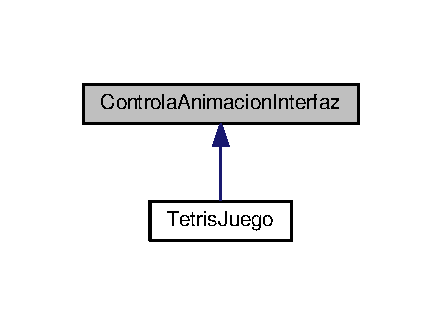
\includegraphics[width=212pt]{class_controla_animacion_interfaz__inherit__graph}
\end{center}
\end{figure}
\subsection*{Public Member Functions}
\begin{DoxyCompactItemize}
\item 
virtual void {\bfseries stopped} (const int Grupo\+Id)\hypertarget{class_controla_animacion_interfaz_a926d0fbba78e151a01bd012e460fbd1d}{}\label{class_controla_animacion_interfaz_a926d0fbba78e151a01bd012e460fbd1d}

\item 
virtual void {\bfseries paused} (\hyperlink{class_simple_animacion}{Simple\+Animacion} $\ast$)\hypertarget{class_controla_animacion_interfaz_a90aa4c3fd3fba7adf01f310548a2b911}{}\label{class_controla_animacion_interfaz_a90aa4c3fd3fba7adf01f310548a2b911}

\item 
virtual void {\bfseries stopped} (const int Grupo\+Id)\hypertarget{class_controla_animacion_interfaz_a926d0fbba78e151a01bd012e460fbd1d}{}\label{class_controla_animacion_interfaz_a926d0fbba78e151a01bd012e460fbd1d}

\item 
virtual void {\bfseries paused} (\hyperlink{class_simple_animacion}{Simple\+Animacion} $\ast$)\hypertarget{class_controla_animacion_interfaz_a90aa4c3fd3fba7adf01f310548a2b911}{}\label{class_controla_animacion_interfaz_a90aa4c3fd3fba7adf01f310548a2b911}

\end{DoxyCompactItemize}


The documentation for this class was generated from the following file\+:\begin{DoxyCompactItemize}
\item 
src/testsotrosjuegos/\+Othello/Controla\+Animacion\+Interfaz.\+hpp\end{DoxyCompactItemize}

\hypertarget{class_control_animacion}{}\section{Control\+Animacion Class Reference}
\label{class_control_animacion}\index{Control\+Animacion@{Control\+Animacion}}
\subsection*{Public Member Functions}
\begin{DoxyCompactItemize}
\item 
{\bfseries Control\+Animacion} (string frames=N\+U\+LL)\hypertarget{class_control_animacion_a6d077c733c0d637f5a27e925f750fac2}{}\label{class_control_animacion_a6d077c733c0d637f5a27e925f750fac2}

\item 
int {\bfseries cuadro} (void)\hypertarget{class_control_animacion_a510c44c25f1d5acaa82ca67e82d52d82}{}\label{class_control_animacion_a510c44c25f1d5acaa82ca67e82d52d82}

\item 
bool {\bfseries es\+\_\+primer\+\_\+cuadro} (void)\hypertarget{class_control_animacion_a73a85ab3fccb53b1457744470daf8ec3}{}\label{class_control_animacion_a73a85ab3fccb53b1457744470daf8ec3}

\item 
bool {\bfseries avanzar} (void)\hypertarget{class_control_animacion_a2be12a01bfdd0ce76fc5a826fa8770ef}{}\label{class_control_animacion_a2be12a01bfdd0ce76fc5a826fa8770ef}

\item 
void {\bfseries reiniciar} (void)\hypertarget{class_control_animacion_a801e3d019765ece628db6626062e4453}{}\label{class_control_animacion_a801e3d019765ece628db6626062e4453}

\item 
void {\bfseries set\+Cuadros} (string frames)\hypertarget{class_control_animacion_a59575c0affda112129413a1983cc7ca5}{}\label{class_control_animacion_a59575c0affda112129413a1983cc7ca5}

\item 
void {\bfseries set\+Inicio\+Animacion} (int nuevo)\hypertarget{class_control_animacion_a59dec38d54106ecfaabbc90db2c1968a}{}\label{class_control_animacion_a59dec38d54106ecfaabbc90db2c1968a}

\end{DoxyCompactItemize}


The documentation for this class was generated from the following files\+:\begin{DoxyCompactItemize}
\item 
src/engine/sprites/animacion/Control\+\_\+\+Animacion.\+hpp\item 
src/engine/sprites/animacion/Control\+\_\+\+Animacion.\+cpp\end{DoxyCompactItemize}

\hypertarget{class_control_player}{}\section{Control\+Player Class Reference}
\label{class_control_player}\index{Control\+Player@{Control\+Player}}
\subsection*{Public Member Functions}
\begin{DoxyCompactItemize}
\item 
{\bfseries Control\+Player} (bool ini=false)\hypertarget{class_control_player_ac3d7c8aa756e72ead84ca6f50f2821fa}{}\label{class_control_player_ac3d7c8aa756e72ead84ca6f50f2821fa}

\item 
void {\bfseries iniciar} ()\hypertarget{class_control_player_a0d545211221da7c7d908520f0f0a9b73}{}\label{class_control_player_a0d545211221da7c7d908520f0f0a9b73}

\item 
bool {\bfseries cargar} (char ruta\mbox{[}$\,$\mbox{]}, bool ini=true)\hypertarget{class_control_player_aaf328fa930e99fc4b3c6b3130c08e0a3}{}\label{class_control_player_aaf328fa930e99fc4b3c6b3130c08e0a3}

\item 
void {\bfseries guardar} (char ruta\mbox{[}$\,$\mbox{]})\hypertarget{class_control_player_a163aa08d30f28910bbd1c2598acfef1b}{}\label{class_control_player_a163aa08d30f28910bbd1c2598acfef1b}

\item 
char $\ast$ {\bfseries get\+Name} (Tecla\+Player tecla)\hypertarget{class_control_player_aa343efdce88d55cc0258f3a5e243a4a8}{}\label{class_control_player_aa343efdce88d55cc0258f3a5e243a4a8}

\item 
bool {\bfseries is\+Boton\+Joystick} (Tecla\+Player tecla)\hypertarget{class_control_player_a17f31058c30a2c352b1642dfed55c537}{}\label{class_control_player_a17f31058c30a2c352b1642dfed55c537}

\item 
bool {\bfseries is\+Direccion\+Joystick} (int tecla)\hypertarget{class_control_player_a78bffce443d2697df26c40a645aa024f}{}\label{class_control_player_a78bffce443d2697df26c40a645aa024f}

\item 
S\+D\+L\+\_\+\+Keycode {\bfseries get\+Key} (Tecla\+Player tecla)\hypertarget{class_control_player_a138c88280be358025ce7747d646b1513}{}\label{class_control_player_a138c88280be358025ce7747d646b1513}

\item 
void {\bfseries set\+Name} (Tecla\+Player tecla, const char name\mbox{[}$\,$\mbox{]})\hypertarget{class_control_player_ae7bb88aea934e2d834877972cf4fa64f}{}\label{class_control_player_ae7bb88aea934e2d834877972cf4fa64f}

\item 
void {\bfseries set\+Is\+Boton\+Joystick} (Tecla\+Player tecla, bool nuevo)\hypertarget{class_control_player_a011f818a1fe293998df18f412e3bb108}{}\label{class_control_player_a011f818a1fe293998df18f412e3bb108}

\item 
void {\bfseries set\+Is\+Direccion\+Joystick} (int tecla, bool nuevo)\hypertarget{class_control_player_a69c332c460a3251782dceb48bb59ca56}{}\label{class_control_player_a69c332c460a3251782dceb48bb59ca56}

\item 
void {\bfseries set\+Key} (Tecla\+Player tecla, S\+D\+L\+\_\+\+Keycode nuevo)\hypertarget{class_control_player_a440681339dfc3b4a32e4bc8dfeeb7df1}{}\label{class_control_player_a440681339dfc3b4a32e4bc8dfeeb7df1}

\item 
void {\bfseries set\+Default\+Keys} (Id\+Player id)\hypertarget{class_control_player_a0df9d15f3e0a45c6b37288c27fc0f7c5}{}\label{class_control_player_a0df9d15f3e0a45c6b37288c27fc0f7c5}

\end{DoxyCompactItemize}


The documentation for this class was generated from the following files\+:\begin{DoxyCompactItemize}
\item 
src/util/control\+\_\+player.\+hpp\item 
src/util/control\+\_\+player.\+cpp\end{DoxyCompactItemize}

\hypertarget{class_control_teclas_player}{}\section{Control\+Teclas\+Player Class Reference}
\label{class_control_teclas_player}\index{Control\+Teclas\+Player@{Control\+Teclas\+Player}}
\subsection*{Public Types}
\begin{DoxyCompactItemize}
\item 
enum {\bfseries Tecla\+Control\+Player} \{ \\*
{\bfseries T\+E\+C\+L\+A\+\_\+\+H\+A\+R\+D\+\_\+\+D\+R\+OP}, 
{\bfseries T\+E\+C\+L\+A\+\_\+\+S\+O\+F\+T\+\_\+\+D\+R\+OP}, 
{\bfseries T\+E\+C\+L\+A\+\_\+\+M\+O\+V\+E\+R\+\_\+\+L\+E\+FT}, 
{\bfseries T\+E\+C\+L\+A\+\_\+\+M\+O\+V\+E\+R\+\_\+\+R\+I\+G\+HT}, 
\\*
{\bfseries T\+E\+C\+L\+A\+\_\+\+G\+I\+R\+A\+R\+\_\+\+L\+E\+FT}, 
{\bfseries T\+E\+C\+L\+A\+\_\+\+G\+I\+R\+A\+R\+\_\+\+R\+I\+G\+HT}, 
{\bfseries T\+E\+C\+L\+A\+\_\+\+P\+A\+U\+SA}, 
{\bfseries N\+\_\+\+T\+E\+C\+L\+AS}
 \}\hypertarget{class_control_teclas_player_aa264a2bfe49cae4380ce7f402a7b67cb}{}\label{class_control_teclas_player_aa264a2bfe49cae4380ce7f402a7b67cb}

\end{DoxyCompactItemize}
\subsection*{Public Member Functions}
\begin{DoxyCompactItemize}
\item 
{\bfseries Control\+Teclas\+Player} (std\+::string ruta\+Archivo\+Key\+Board)\hypertarget{class_control_teclas_player_aace524629cc9503e1cdb884da0f9c024}{}\label{class_control_teclas_player_aace524629cc9503e1cdb884da0f9c024}

\item 
void {\bfseries establecer\+Valor\+Default} ()\hypertarget{class_control_teclas_player_ae335e0af8196ab2c38b1d689c7f60892}{}\label{class_control_teclas_player_ae335e0af8196ab2c38b1d689c7f60892}

\item 
void {\bfseries update} (const Uint8 $\ast$\+\_\+teclas)\hypertarget{class_control_teclas_player_a6e18cbcf904086253e2bae1577f17b3b}{}\label{class_control_teclas_player_a6e18cbcf904086253e2bae1577f17b3b}

\item 
bool {\bfseries esta\+Tecla\+Aceptada} (Tecla\+Control\+Player tecla)\hypertarget{class_control_teclas_player_afeb71f0b1714db702bafdf2030d804df}{}\label{class_control_teclas_player_afeb71f0b1714db702bafdf2030d804df}

\item 
bool {\bfseries esta\+Tecla\+Presionada} (Tecla\+Control\+Player tecla)\hypertarget{class_control_teclas_player_aeff153841059f65c21fcd5e862a138b8}{}\label{class_control_teclas_player_aeff153841059f65c21fcd5e862a138b8}

\end{DoxyCompactItemize}


The documentation for this class was generated from the following file\+:\begin{DoxyCompactItemize}
\item 
src/testsotrosjuegos/\+Tetris/Control\+Teclas\+Player.\+hpp\end{DoxyCompactItemize}

\hypertarget{struct_t_m_x_1_1_parser_1_1_data}{}\section{T\+MX\+:\+:Parser\+:\+:Data Struct Reference}
\label{struct_t_m_x_1_1_parser_1_1_data}\index{T\+M\+X\+::\+Parser\+::\+Data@{T\+M\+X\+::\+Parser\+::\+Data}}
\subsection*{Public Attributes}
\begin{DoxyCompactItemize}
\item 
std\+::string {\bfseries encoding}\hypertarget{struct_t_m_x_1_1_parser_1_1_data_a81a5cc3399b2675d6621ee7865f0a4f8}{}\label{struct_t_m_x_1_1_parser_1_1_data_a81a5cc3399b2675d6621ee7865f0a4f8}

\item 
std\+::string {\bfseries compression}\hypertarget{struct_t_m_x_1_1_parser_1_1_data_aebdceea109a2e11022a708cdd2a6595c}{}\label{struct_t_m_x_1_1_parser_1_1_data_aebdceea109a2e11022a708cdd2a6595c}

\item 
std\+::string {\bfseries contents}\hypertarget{struct_t_m_x_1_1_parser_1_1_data_ace1c81445b2f9ababe1f334c0706e409}{}\label{struct_t_m_x_1_1_parser_1_1_data_ace1c81445b2f9ababe1f334c0706e409}

\end{DoxyCompactItemize}


The documentation for this struct was generated from the following file\+:\begin{DoxyCompactItemize}
\item 
src/engine/mapa/include/T\+M\+X\+Parser.\+h\end{DoxyCompactItemize}

\hypertarget{class_draw_group}{}\section{Draw\+Group Class Reference}
\label{class_draw_group}\index{Draw\+Group@{Draw\+Group}}


Inheritance diagram for Draw\+Group\+:\nopagebreak
\begin{figure}[H]
\begin{center}
\leavevmode
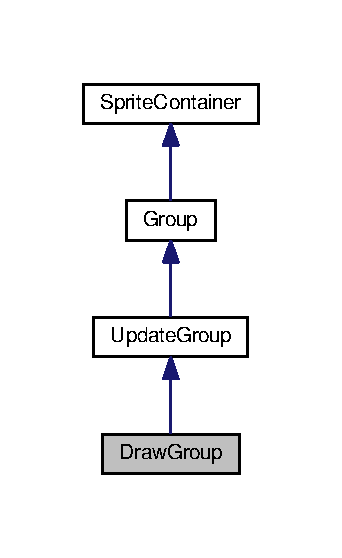
\includegraphics[width=164pt]{class_draw_group__inherit__graph}
\end{center}
\end{figure}


Collaboration diagram for Draw\+Group\+:\nopagebreak
\begin{figure}[H]
\begin{center}
\leavevmode
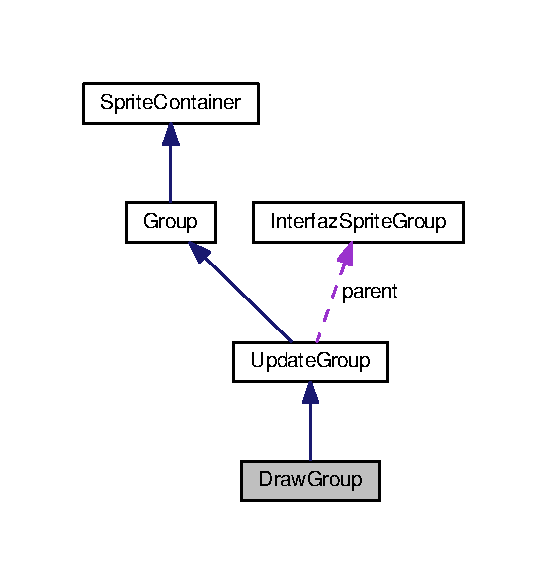
\includegraphics[width=263pt]{class_draw_group__coll__graph}
\end{center}
\end{figure}
\subsection*{Public Member Functions}
\begin{DoxyCompactItemize}
\item 
{\bfseries Draw\+Group} (\hyperlink{class_interfaz_sprite_group}{Interfaz\+Sprite\+Group} $\ast$parent)\hypertarget{class_draw_group_a985c396afbae3c1686c2fd65288b7443}{}\label{class_draw_group_a985c396afbae3c1686c2fd65288b7443}

\item 
void {\bfseries draw} (S\+D\+L\+\_\+\+Renderer $\ast$gr)\hypertarget{class_draw_group_ad658a4bc0093f182af2fa41883f99b07}{}\label{class_draw_group_ad658a4bc0093f182af2fa41883f99b07}

\end{DoxyCompactItemize}
\subsection*{Additional Inherited Members}


The documentation for this class was generated from the following file\+:\begin{DoxyCompactItemize}
\item 
src/engine/sprites/C\+Draw\+Group.\+hpp\end{DoxyCompactItemize}

\hypertarget{class_editor}{}\section{Editor Class Reference}
\label{class_editor}\index{Editor@{Editor}}


Inheritance diagram for Editor\+:\nopagebreak
\begin{figure}[H]
\begin{center}
\leavevmode
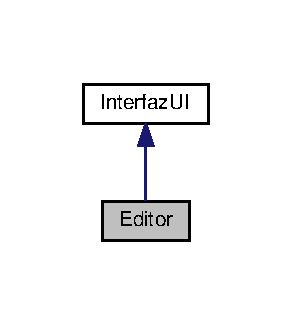
\includegraphics[width=140pt]{class_editor__inherit__graph}
\end{center}
\end{figure}


Collaboration diagram for Editor\+:\nopagebreak
\begin{figure}[H]
\begin{center}
\leavevmode
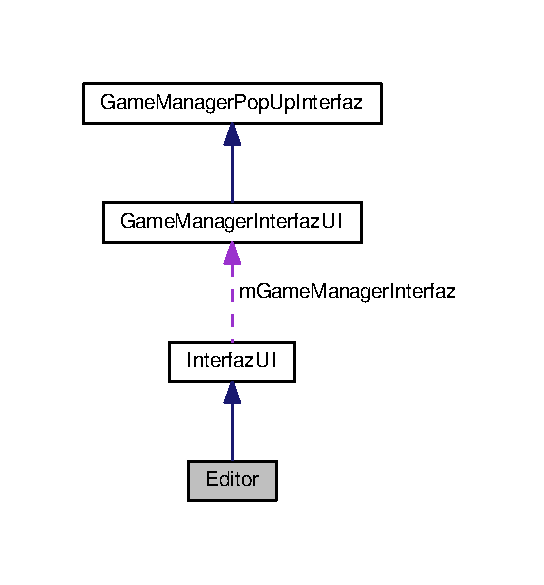
\includegraphics[width=261pt]{class_editor__coll__graph}
\end{center}
\end{figure}
\subsection*{Additional Inherited Members}


The documentation for this class was generated from the following file\+:\begin{DoxyCompactItemize}
\item 
src/\+Interfaces/editor/editor.\+hpp\end{DoxyCompactItemize}

\hypertarget{class_explosion}{}\section{Explosion Class Reference}
\label{class_explosion}\index{Explosion@{Explosion}}


Inheritance diagram for Explosion\+:\nopagebreak
\begin{figure}[H]
\begin{center}
\leavevmode
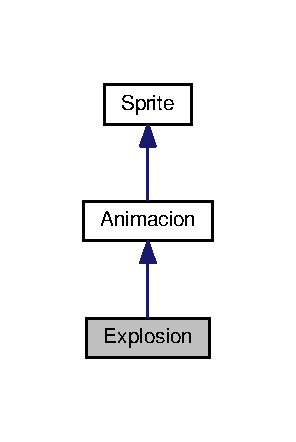
\includegraphics[width=142pt]{class_explosion__inherit__graph}
\end{center}
\end{figure}


Collaboration diagram for Explosion\+:\nopagebreak
\begin{figure}[H]
\begin{center}
\leavevmode
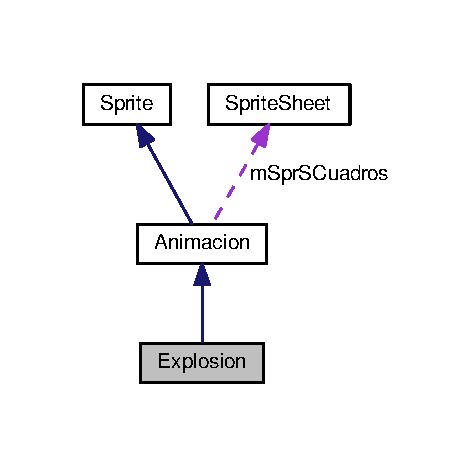
\includegraphics[width=227pt]{class_explosion__coll__graph}
\end{center}
\end{figure}
\subsection*{Public Member Functions}
\begin{DoxyCompactItemize}
\item 
{\bfseries Explosion} (\hyperlink{class_interfaz_juego}{Interfaz\+Juego} $\ast$juego, S\+D\+L\+\_\+\+Renderer $\ast$g\+Renderer, \hyperlink{class_player}{Player} $\ast$player\+Lanzador)\hypertarget{class_explosion_a85068ed7729f0ad179fb7c764f96c0b1}{}\label{class_explosion_a85068ed7729f0ad179fb7c764f96c0b1}

\item 
void {\bfseries draw} (S\+D\+L\+\_\+\+Renderer $\ast$g\+Renderer)\hypertarget{class_explosion_ad93f3cca36426268c06a1c832c4ad7f8}{}\label{class_explosion_ad93f3cca36426268c06a1c832c4ad7f8}

\item 
bool {\bfseries colision} (S\+D\+L\+\_\+\+Rect \&rect\+\_\+coli)\hypertarget{class_explosion_a91dcbc01a6178dbb5e66a6209214aa56}{}\label{class_explosion_a91dcbc01a6178dbb5e66a6209214aa56}

\item 
void {\bfseries detectar\+Alcances} ()\hypertarget{class_explosion_aa381f273160b625c9a37e40e1ae0cda3}{}\label{class_explosion_aa381f273160b625c9a37e40e1ae0cda3}

\item 
\hyperlink{class_player}{Player} $\ast$ {\bfseries get\+Creador} ()\hypertarget{class_explosion_a8be576e77e5074fb3de9f6951d0887e1}{}\label{class_explosion_a8be576e77e5074fb3de9f6951d0887e1}

\end{DoxyCompactItemize}
\subsection*{Additional Inherited Members}


The documentation for this class was generated from the following files\+:\begin{DoxyCompactItemize}
\item 
src/objetos/explosion.\+hpp\item 
src/objetos/explosion.\+cpp\end{DoxyCompactItemize}

\hypertarget{classrapidxml_1_1file}{}\section{rapidxml\+:\+:file$<$ Ch $>$ Class Template Reference}
\label{classrapidxml_1_1file}\index{rapidxml\+::file$<$ Ch $>$@{rapidxml\+::file$<$ Ch $>$}}


Represents data loaded from a file.  




{\ttfamily \#include $<$rapidxml\+\_\+utils.\+hpp$>$}

\subsection*{Public Member Functions}
\begin{DoxyCompactItemize}
\item 
\hyperlink{classrapidxml_1_1file_ae881a3cab1fe7152d45c92a8d7606cb3}{file} (const char $\ast$filename)
\item 
\hyperlink{classrapidxml_1_1file_a90707ccd991cc392dcf4bef37eed9d1f}{file} (std\+::basic\+\_\+istream$<$ Ch $>$ \&stream)
\item 
Ch $\ast$ \hyperlink{classrapidxml_1_1file_af1c71d65862c7af14e4708e32a80c1de}{data} ()
\item 
const Ch $\ast$ \hyperlink{classrapidxml_1_1file_aceb8f5ebd577c946a74b1ea3e2e0c576}{data} () const 
\item 
std\+::size\+\_\+t \hyperlink{classrapidxml_1_1file_a20191d167c6e00a88a44ca9a3a54e1c5}{size} () const 
\end{DoxyCompactItemize}


\subsection{Detailed Description}
\subsubsection*{template$<$class Ch = char$>$\\*
class rapidxml\+::file$<$ Ch $>$}

Represents data loaded from a file. 

\subsection{Constructor \& Destructor Documentation}
\index{rapidxml\+::file@{rapidxml\+::file}!file@{file}}
\index{file@{file}!rapidxml\+::file@{rapidxml\+::file}}
\subsubsection[{\texorpdfstring{file(const char $\ast$filename)}{file(const char *filename)}}]{\setlength{\rightskip}{0pt plus 5cm}template$<$class Ch  = char$>$ {\bf rapidxml\+::file}$<$ Ch $>$\+::{\bf file} (
\begin{DoxyParamCaption}
\item[{const char $\ast$}]{filename}
\end{DoxyParamCaption}
)\hspace{0.3cm}{\ttfamily [inline]}}\hypertarget{classrapidxml_1_1file_ae881a3cab1fe7152d45c92a8d7606cb3}{}\label{classrapidxml_1_1file_ae881a3cab1fe7152d45c92a8d7606cb3}
Loads file into the memory. Data will be automatically destroyed by the destructor. 
\begin{DoxyParams}{Parameters}
{\em filename} & Filename to load. \\
\hline
\end{DoxyParams}
\index{rapidxml\+::file@{rapidxml\+::file}!file@{file}}
\index{file@{file}!rapidxml\+::file@{rapidxml\+::file}}
\subsubsection[{\texorpdfstring{file(std\+::basic\+\_\+istream$<$ Ch $>$ \&stream)}{file(std::basic_istream< Ch > &stream)}}]{\setlength{\rightskip}{0pt plus 5cm}template$<$class Ch  = char$>$ {\bf rapidxml\+::file}$<$ Ch $>$\+::{\bf file} (
\begin{DoxyParamCaption}
\item[{std\+::basic\+\_\+istream$<$ Ch $>$ \&}]{stream}
\end{DoxyParamCaption}
)\hspace{0.3cm}{\ttfamily [inline]}}\hypertarget{classrapidxml_1_1file_a90707ccd991cc392dcf4bef37eed9d1f}{}\label{classrapidxml_1_1file_a90707ccd991cc392dcf4bef37eed9d1f}
Loads file into the memory. Data will be automatically destroyed by the destructor 
\begin{DoxyParams}{Parameters}
{\em stream} & Stream to load from \\
\hline
\end{DoxyParams}


\subsection{Member Function Documentation}
\index{rapidxml\+::file@{rapidxml\+::file}!data@{data}}
\index{data@{data}!rapidxml\+::file@{rapidxml\+::file}}
\subsubsection[{\texorpdfstring{data()}{data()}}]{\setlength{\rightskip}{0pt plus 5cm}template$<$class Ch  = char$>$ Ch$\ast$ {\bf rapidxml\+::file}$<$ Ch $>$\+::data (
\begin{DoxyParamCaption}
{}
\end{DoxyParamCaption}
)\hspace{0.3cm}{\ttfamily [inline]}}\hypertarget{classrapidxml_1_1file_af1c71d65862c7af14e4708e32a80c1de}{}\label{classrapidxml_1_1file_af1c71d65862c7af14e4708e32a80c1de}
Gets file data. \begin{DoxyReturn}{Returns}
Pointer to data of file. 
\end{DoxyReturn}
\index{rapidxml\+::file@{rapidxml\+::file}!data@{data}}
\index{data@{data}!rapidxml\+::file@{rapidxml\+::file}}
\subsubsection[{\texorpdfstring{data() const }{data() const }}]{\setlength{\rightskip}{0pt plus 5cm}template$<$class Ch  = char$>$ const Ch$\ast$ {\bf rapidxml\+::file}$<$ Ch $>$\+::data (
\begin{DoxyParamCaption}
{}
\end{DoxyParamCaption}
) const\hspace{0.3cm}{\ttfamily [inline]}}\hypertarget{classrapidxml_1_1file_aceb8f5ebd577c946a74b1ea3e2e0c576}{}\label{classrapidxml_1_1file_aceb8f5ebd577c946a74b1ea3e2e0c576}
Gets file data. \begin{DoxyReturn}{Returns}
Pointer to data of file. 
\end{DoxyReturn}
\index{rapidxml\+::file@{rapidxml\+::file}!size@{size}}
\index{size@{size}!rapidxml\+::file@{rapidxml\+::file}}
\subsubsection[{\texorpdfstring{size() const }{size() const }}]{\setlength{\rightskip}{0pt plus 5cm}template$<$class Ch  = char$>$ std\+::size\+\_\+t {\bf rapidxml\+::file}$<$ Ch $>$\+::size (
\begin{DoxyParamCaption}
{}
\end{DoxyParamCaption}
) const\hspace{0.3cm}{\ttfamily [inline]}}\hypertarget{classrapidxml_1_1file_a20191d167c6e00a88a44ca9a3a54e1c5}{}\label{classrapidxml_1_1file_a20191d167c6e00a88a44ca9a3a54e1c5}
Gets file data size. \begin{DoxyReturn}{Returns}
Size of file data, in characters. 
\end{DoxyReturn}


The documentation for this class was generated from the following file\+:\begin{DoxyCompactItemize}
\item 
src/engine/mapa/include/rapidxml/\hyperlink{rapidxml__utils_8hpp}{rapidxml\+\_\+utils.\+hpp}\end{DoxyCompactItemize}

\hypertarget{class_galeria}{}\section{Galeria Class Reference}
\label{class_galeria}\index{Galeria@{Galeria}}
\subsection*{Public Types}
\begin{DoxyCompactItemize}
\item 
enum {\bfseries Code\+Music\+Efecto} \{ \\*
{\bfseries S\+F\+X\+\_\+\+C\+O\+G\+E\+R\+\_\+\+I\+T\+EM}, 
{\bfseries S\+F\+X\+\_\+\+T\+O\+N\+O\+\_\+\+A\+C\+U\+A\+T\+I\+CO}, 
{\bfseries S\+F\+X\+\_\+\+T\+O\+N\+O\+\_\+\+S\+E\+CO}, 
{\bfseries S\+F\+X\+\_\+\+C\+A\+M\+P\+A\+N\+A\+DA}, 
\\*
{\bfseries S\+F\+X\+\_\+\+E\+X\+P\+L\+O\+S\+I\+ON}, 
{\bfseries S\+F\+X\+\_\+\+E\+S\+T\+R\+A\+N\+YO}, 
{\bfseries S\+F\+X\+\_\+\+P\+I\+E\+R\+D\+E\+\_\+\+V\+I\+DA}, 
{\bfseries \+\_\+\+E\+F\+E\+C\+T\+OS}
 \}\hypertarget{class_galeria_a5545af8ffe889df8033ea5ac09d8f61d}{}\label{class_galeria_a5545af8ffe889df8033ea5ac09d8f61d}

\item 
enum {\bfseries Code\+Music\+Sonido} \{ \\*
{\bfseries S\+N\+D\+\_\+\+M\+E\+NU} =0, 
{\bfseries S\+N\+D\+\_\+\+E\+D\+I\+T\+OR} =1, 
{\bfseries S\+N\+D\+\_\+\+L\+E\+V\+E\+L\+\_\+\+S\+T\+A\+RT} =2, 
{\bfseries S\+N\+D\+\_\+\+W\+A\+R\+N\+I\+N\+G\+\_\+\+T\+I\+ME} =3, 
\\*
{\bfseries S\+N\+D\+\_\+\+I\+N\+\_\+\+G\+A\+M\+E\+\_\+1} =4, 
{\bfseries S\+N\+D\+\_\+\+I\+N\+\_\+\+G\+A\+M\+E\+\_\+2} =5, 
{\bfseries \+\_\+\+S\+O\+N\+I\+D\+OS}
 \}\hypertarget{class_galeria_a3f36d29a45086825cf197f043e1bf810}{}\label{class_galeria_a3f36d29a45086825cf197f043e1bf810}

\item 
enum {\bfseries Code\+Imagen} \{ \\*
{\bfseries I\+M\+G\+\_\+\+G\+L\+O\+BO}, 
{\bfseries I\+M\+G\+\_\+\+P\+L\+A\+Y\+E\+R\+\_\+1}, 
{\bfseries I\+M\+G\+\_\+\+P\+L\+A\+Y\+E\+R\+\_\+2}, 
{\bfseries I\+M\+G\+\_\+\+P\+L\+A\+Y\+E\+R\+\_\+3}, 
\\*
{\bfseries I\+M\+G\+\_\+\+P\+L\+A\+Y\+E\+R\+\_\+4}, 
{\bfseries I\+M\+G\+\_\+\+P\+L\+A\+Y\+E\+R\+\_\+5}, 
{\bfseries I\+M\+G\+\_\+\+P\+L\+A\+Y\+E\+R\+\_\+1\+\_\+\+M\+U\+R\+I\+E\+N\+DO}, 
{\bfseries I\+M\+G\+\_\+\+P\+L\+A\+Y\+E\+R\+\_\+2\+\_\+\+M\+U\+R\+I\+E\+N\+DO}, 
\\*
{\bfseries I\+M\+G\+\_\+\+P\+L\+A\+Y\+E\+R\+\_\+3\+\_\+\+M\+U\+R\+I\+E\+N\+DO}, 
{\bfseries I\+M\+G\+\_\+\+P\+L\+A\+Y\+E\+R\+\_\+4\+\_\+\+M\+U\+R\+I\+E\+N\+DO}, 
{\bfseries I\+M\+G\+\_\+\+P\+L\+A\+Y\+E\+R\+\_\+5\+\_\+\+M\+U\+R\+I\+E\+N\+DO}, 
{\bfseries I\+M\+G\+\_\+\+F\+O\+N\+D\+O\+\_\+\+M\+E\+NU}, 
\\*
{\bfseries I\+M\+G\+\_\+\+F\+O\+N\+D\+O\+\_\+\+C\+R\+E\+D\+I\+T\+OS}, 
{\bfseries I\+M\+G\+\_\+\+F\+O\+N\+D\+O\+\_\+\+E\+D\+I\+T\+O\+R\+\_\+\+S\+E\+L\+E\+C\+T\+\_\+\+F\+I\+LE}, 
{\bfseries I\+M\+G\+\_\+\+F\+O\+N\+D\+O\+\_\+\+P\+A\+R\+TI}, 
{\bfseries I\+M\+G\+\_\+\+F\+O\+N\+D\+O\+\_\+\+E\+D\+I\+F\+I\+C\+I\+OS}, 
\\*
{\bfseries I\+M\+G\+\_\+\+F\+O\+N\+D\+O\+\_\+\+M\+E\+T\+AL}, 
{\bfseries I\+M\+G\+\_\+\+F\+O\+N\+D\+O\+\_\+\+N\+E\+G\+RO}, 
{\bfseries I\+M\+G\+\_\+\+F\+O\+N\+D\+O\+\_\+\+B\+L\+A\+N\+CO}, 
{\bfseries I\+M\+G\+\_\+\+F\+U\+E\+N\+T\+E\+\_\+1}, 
\\*
{\bfseries I\+M\+G\+\_\+\+F\+U\+E\+N\+T\+E\+\_\+2}, 
{\bfseries I\+M\+G\+\_\+\+F\+U\+E\+N\+T\+E\+\_\+3}, 
{\bfseries I\+M\+G\+\_\+\+F\+U\+E\+N\+T\+E\+\_\+4}, 
{\bfseries I\+M\+G\+\_\+\+F\+U\+E\+N\+T\+E\+\_\+5}, 
\\*
{\bfseries I\+M\+G\+\_\+\+F\+U\+E\+N\+T\+E\+\_\+6}, 
{\bfseries I\+M\+G\+\_\+\+F\+U\+E\+N\+T\+E\+\_\+7}, 
{\bfseries I\+M\+G\+\_\+\+F\+U\+E\+N\+T\+E\+\_\+8}, 
{\bfseries I\+M\+G\+\_\+\+T\+X\+T\+\_\+\+P\+U\+N\+T\+A\+JE}, 
\\*
{\bfseries I\+M\+G\+\_\+\+T\+X\+T\+\_\+\+P\+R\+E\+S\+I\+O\+N\+A\+\_\+\+S\+T\+A\+RT}, 
{\bfseries I\+M\+G\+\_\+\+T\+X\+T\+\_\+\+T\+I\+L\+ES}, 
{\bfseries I\+M\+G\+\_\+\+T\+X\+T\+\_\+\+A\+R\+R\+I\+BA}, 
{\bfseries I\+M\+G\+\_\+\+T\+X\+T\+\_\+\+A\+B\+A\+JO}, 
\\*
{\bfseries I\+M\+G\+\_\+\+T\+X\+T\+\_\+\+I\+Z\+Q\+U\+I\+E\+R\+DA}, 
{\bfseries I\+M\+G\+\_\+\+T\+X\+T\+\_\+\+D\+E\+R\+E\+C\+HA}, 
{\bfseries I\+M\+G\+\_\+\+T\+X\+T\+\_\+\+A\+C\+C\+I\+ON}, 
{\bfseries I\+M\+G\+\_\+\+T\+X\+T\+\_\+\+S\+T\+A\+RT}, 
\\*
{\bfseries I\+M\+G\+\_\+\+T\+X\+T\+\_\+\+V\+I\+C\+T\+O\+R\+I\+AS}, 
{\bfseries I\+M\+G\+\_\+\+T\+X\+T\+\_\+\+A\+C\+T\+I\+V\+A\+DO}, 
{\bfseries I\+M\+G\+\_\+\+T\+X\+T\+\_\+\+P\+L\+A\+Y\+E\+R\+S\+\_\+\+E\+N\+\_\+\+B\+A\+T\+A\+L\+LA}, 
{\bfseries I\+M\+G\+\_\+\+T\+X\+T\+\_\+\+P\+R\+E\+S\+I\+O\+N\+A\+\_\+\+A\+C\+C\+I\+ON}, 
\\*
{\bfseries I\+M\+G\+\_\+\+T\+X\+T\+\_\+\+P\+R\+E\+S\+I\+O\+NA}, 
{\bfseries I\+M\+G\+\_\+\+T\+X\+T\+\_\+\+T\+I\+E\+M\+P\+O\+\_\+\+P\+O\+R\+\_\+\+R\+O\+N\+DA}, 
{\bfseries I\+M\+G\+\_\+\+T\+X\+T\+\_\+\+S\+C\+O\+R\+E\+B\+O\+A\+RD}, 
{\bfseries I\+M\+G\+\_\+\+B\+O\+T\+O\+N\+\_\+\+A\+C\+T\+I\+V\+A\+D\+O\+\_\+\+D\+E\+S\+A\+C\+T\+I\+V\+A\+DO}, 
\\*
{\bfseries I\+M\+G\+\_\+\+B\+O\+T\+O\+N\+\_\+\+J\+U\+G\+AR}, 
{\bfseries I\+M\+G\+\_\+\+B\+O\+T\+O\+N\+\_\+\+E\+S\+T\+R\+A\+N\+IO}, 
{\bfseries I\+M\+G\+\_\+\+B\+O\+T\+O\+N\+\_\+\+C\+A\+M\+B\+I\+AR}, 
{\bfseries I\+M\+G\+\_\+\+B\+O\+T\+O\+N\+\_\+\+G\+U\+A\+R\+D\+AR}, 
\\*
{\bfseries I\+M\+G\+\_\+\+B\+O\+T\+O\+N\+\_\+\+B\+O\+R\+R\+A\+R\+\_\+\+M\+A\+PA}, 
{\bfseries I\+M\+G\+\_\+\+B\+O\+T\+O\+N\+\_\+\+F\+L\+E\+C\+H\+A\+\_\+\+P\+E\+Q\+U\+E\+\_\+\+D\+E\+R\+E\+C\+HA}, 
{\bfseries I\+M\+G\+\_\+\+B\+O\+T\+O\+N\+\_\+\+M\+AS}, 
{\bfseries I\+M\+G\+\_\+\+B\+O\+T\+O\+N\+\_\+\+M\+E\+N\+OS}, 
\\*
{\bfseries I\+M\+G\+\_\+\+B\+O\+T\+O\+N\+\_\+\+F\+L\+E\+C\+H\+A\+\_\+\+G\+R\+A\+N\+D\+E\+\_\+\+I\+Z\+Q\+U\+I\+E\+R\+DA}, 
{\bfseries I\+M\+G\+\_\+\+B\+O\+T\+O\+N\+\_\+\+F\+L\+E\+C\+H\+A\+\_\+\+G\+R\+A\+N\+D\+E\+\_\+\+D\+E\+R\+E\+C\+HA}, 
{\bfseries I\+M\+G\+\_\+\+B\+O\+T\+O\+N\+\_\+\+P\+L\+A\+Y\+E\+R\+\_\+1}, 
{\bfseries I\+M\+G\+\_\+\+B\+O\+T\+O\+N\+\_\+\+P\+L\+A\+Y\+E\+R\+\_\+2}, 
\\*
{\bfseries I\+M\+G\+\_\+\+B\+O\+T\+O\+N\+\_\+\+P\+L\+A\+Y\+E\+R\+\_\+3}, 
{\bfseries I\+M\+G\+\_\+\+B\+O\+T\+O\+N\+\_\+\+P\+L\+A\+Y\+E\+R\+\_\+4}, 
{\bfseries I\+M\+G\+\_\+\+B\+O\+T\+O\+N\+\_\+\+P\+L\+A\+Y\+E\+R\+\_\+5}, 
{\bfseries I\+M\+G\+\_\+\+B\+O\+T\+O\+N\+\_\+\+C\+A\+M\+B\+I\+A\+R\+\_\+\+M\+A\+PA}, 
\\*
{\bfseries I\+M\+G\+\_\+\+B\+O\+T\+O\+N\+\_\+\+J\+U\+G\+A\+R\+\_\+2}, 
{\bfseries I\+M\+G\+\_\+\+T\+A\+B\+L\+E\+RO}, 
{\bfseries I\+M\+G\+\_\+\+B\+L\+O\+Q\+U\+E\+S\+\_\+\+F\+I\+RE}, 
{\bfseries I\+M\+G\+\_\+\+I\+T\+E\+M\+\_\+\+F\+I\+RE}, 
\\*
{\bfseries I\+M\+G\+\_\+\+G\+U\+I\+\_\+\+I\+N\+P\+U\+T\+\_\+\+T\+E\+XT}, 
{\bfseries I\+M\+G\+\_\+\+T\+A\+B\+L\+A\+\_\+\+K\+I\+L\+LS}, 
{\bfseries I\+M\+G\+\_\+\+C\+A\+R\+A\+S\+\_\+\+B\+O\+M\+B\+E\+R\+M\+AN}, 
{\bfseries I\+M\+G\+\_\+\+C\+A\+R\+A\+S\+\_\+\+B\+O\+M\+B\+E\+R\+M\+A\+N\+\_\+\+G\+R\+A\+N\+D\+ES}, 
\\*
{\bfseries I\+M\+G\+\_\+\+B\+O\+M\+BA}, 
{\bfseries I\+M\+G\+\_\+\+I\+T\+EM}, 
{\bfseries I\+M\+G\+\_\+\+E\+X\+P\+L\+O\+S\+I\+ON}, 
{\bfseries I\+M\+G\+\_\+\+C\+U\+A\+D\+R\+O\+\_\+\+P\+E\+Q\+U\+E\+N\+IO}, 
\\*
{\bfseries I\+M\+G\+\_\+\+C\+U\+A\+D\+R\+O\+\_\+\+M\+E\+D\+I\+A\+NO}, 
{\bfseries I\+M\+G\+\_\+\+C\+U\+A\+D\+R\+O\+\_\+\+G\+R\+A\+N\+DE}, 
{\bfseries I\+M\+G\+\_\+\+L\+L\+A\+MA}, 
{\bfseries I\+M\+G\+\_\+\+B\+O\+M\+B\+A\+\_\+\+P\+E\+Q\+UE}, 
\\*
{\bfseries I\+M\+G\+\_\+\+C\+O\+R\+A\+Z\+ON}, 
{\bfseries I\+M\+G\+\_\+\+P\+R\+E\+G\+U\+N\+TA}, 
{\bfseries I\+M\+G\+\_\+\+T\+I\+L\+ES}, 
{\bfseries I\+M\+G\+\_\+\+T\+R\+O\+F\+EO}, 
\\*
{\bfseries I\+M\+G\+\_\+\+C\+U\+A\+D\+R\+O\+\_\+\+S\+C\+O\+R\+E\+B\+O\+A\+RD}, 
{\bfseries \+\_\+\+I\+M\+A\+G\+E\+N\+ES}
 \}\hypertarget{class_galeria_a4d8d723f9fa027d3ed8dec680d8a57a9}{}\label{class_galeria_a4d8d723f9fa027d3ed8dec680d8a57a9}

\end{DoxyCompactItemize}
\subsection*{Public Member Functions}
\begin{DoxyCompactItemize}
\item 
\hyperlink{class_l_texture}{L\+Texture} $\ast$ {\bfseries get\+Imagen} (Code\+Imagen code)\hypertarget{class_galeria_a2effd1fed7eb30b0258ddca113891af8}{}\label{class_galeria_a2effd1fed7eb30b0258ddca113891af8}

\item 
Mix\+\_\+\+Chunk $\ast$ {\bfseries get\+Music\+Efecto} (Code\+Music\+Efecto code)\hypertarget{class_galeria_a008113f3eae096c2a02154ddaae5152b}{}\label{class_galeria_a008113f3eae096c2a02154ddaae5152b}

\item 
Mix\+\_\+\+Music $\ast$ {\bfseries get\+Music\+Sonido} (Code\+Music\+Sonido code)\hypertarget{class_galeria_aad0b599a285380784600e34eaabb01ed}{}\label{class_galeria_aad0b599a285380784600e34eaabb01ed}

\item 
bool {\bfseries cargar\+Texturas} (S\+D\+L\+\_\+\+Renderer $\ast$g\+Renderer, string ruta\+Texturas)\hypertarget{class_galeria_ac2dafe4ff2618f306b19f929a34fbe66}{}\label{class_galeria_ac2dafe4ff2618f306b19f929a34fbe66}

\item 
bool {\bfseries cargar\+Sonidos} (string ruta\+Sonidos)\hypertarget{class_galeria_a2921ac0b56f2b895f1ab7f4293487942}{}\label{class_galeria_a2921ac0b56f2b895f1ab7f4293487942}

\end{DoxyCompactItemize}


The documentation for this class was generated from the following files\+:\begin{DoxyCompactItemize}
\item 
src/engine/util/galeria.\+hpp\item 
src/engine/util/galeria.\+cpp\end{DoxyCompactItemize}

\hypertarget{class_game_manager}{}\section{Game\+Manager Class Reference}
\label{class_game_manager}\index{Game\+Manager@{Game\+Manager}}


{\ttfamily \#include $<$game\+\_\+manager.\+hpp$>$}



Inheritance diagram for Game\+Manager\+:\nopagebreak
\begin{figure}[H]
\begin{center}
\leavevmode
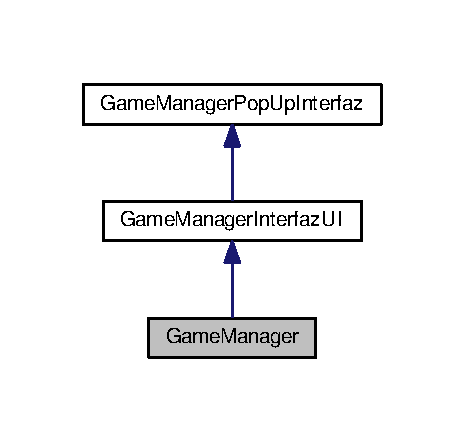
\includegraphics[width=223pt]{class_game_manager__inherit__graph}
\end{center}
\end{figure}


Collaboration diagram for Game\+Manager\+:\nopagebreak
\begin{figure}[H]
\begin{center}
\leavevmode
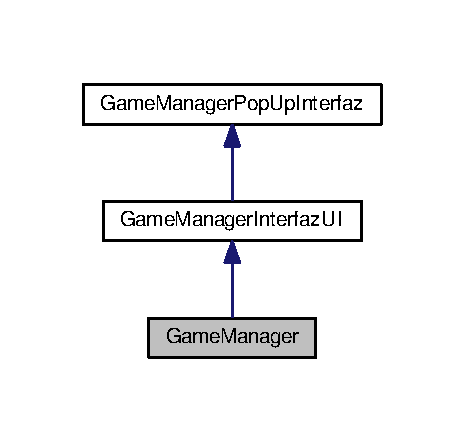
\includegraphics[width=223pt]{class_game_manager__coll__graph}
\end{center}
\end{figure}
\subsection*{Public Member Functions}
\begin{DoxyCompactItemize}
\item 
\hyperlink{class_game_manager_ad42e6937ed9cacf6570a002a6a7abb56}{Game\+Manager} (std\+::string caption, std\+::string ruta\+\_\+icono, unsigned int witdth, unsigned int height, bool pantalla\+Completa)
\item 
void \hyperlink{class_game_manager_aeaaa62ac9dff043fb89932663744d7ea}{iniciar\+Libreria\+S\+DL} ()
\item 
void \hyperlink{class_game_manager_a215db619b1bc7d33fd0286fd3dc58000}{establecer\+Modo\+De\+Video} (bool pantalla\+\_\+completa=false)
\item 
void \hyperlink{class_game_manager_ac40f7fb97ee52c4a4a9361aca98dfac5}{activar\+Joysticks} ()
\item 
S\+D\+L\+\_\+\+Joystick $\ast$ \hyperlink{class_game_manager_a9bb21d9af524ae6c72bdd8dc109ce957}{get\+Joy} (int id)
\item 
int \hyperlink{class_game_manager_ae47edae1e15eaf1d4624cc4e66a9f559}{get\+Active\+Joys} ()
\item 
void \hyperlink{class_game_manager_a1a7ef9efef7dffba5887409b2008f833}{cambiar\+Interfaz} (\hyperlink{class_interfaz_u_i}{Interfaz\+UI} $\ast$nueva)
\item 
bool \hyperlink{class_game_manager_aeb38bf2a7f818f76f79f30bce0a72f57}{procesar\+Eventos} ()
\item 
void \hyperlink{class_game_manager_abbde8090c24ca199815ba1e85059c96f}{run} ()
\item 
void {\bfseries quit} ()\hypertarget{class_game_manager_ac63aa477ce3707e03b42968d364a6ce6}{}\label{class_game_manager_ac63aa477ce3707e03b42968d364a6ce6}

\item 
void \hyperlink{class_game_manager_ae693cf42cfb96a0bb6d7de8fad55739d}{play} (Galeria\+::\+Code\+Music\+Efecto code) override
\item 
void \hyperlink{class_game_manager_a55482db663320dd82b11bb221049bd98}{play\+Sound} (Galeria\+::\+Code\+Music\+Sonido code) override
\item 
\hyperlink{class_l_texture}{L\+Texture} $\ast$ {\bfseries get\+Texture} (Galeria\+::\+Code\+Imagen code) override\hypertarget{class_game_manager_aafcc260a50dd3fa22e8e9fd926997418}{}\label{class_game_manager_aafcc260a50dd3fa22e8e9fd926997418}

\item 
int {\bfseries get\+Width} ()\hypertarget{class_game_manager_ab07784212df355b8820b3b8409540fc9}{}\label{class_game_manager_ab07784212df355b8820b3b8409540fc9}

\item 
int {\bfseries get\+Height} ()\hypertarget{class_game_manager_ac4640c4a2aa0af055a3956fb64e367fb}{}\label{class_game_manager_ac4640c4a2aa0af055a3956fb64e367fb}

\item 
void \hyperlink{class_game_manager_aaa4c8097c4e4288282a261e09ceebcb8}{go\+Back} ()
\item 
void {\bfseries set\+Root} (\hyperlink{class_interfaz_u_i}{Interfaz\+UI} $\ast$nueva\+Interfaz\+Root)\hypertarget{class_game_manager_a6528d38df521ce4915cd9a4aa11ed274}{}\label{class_game_manager_a6528d38df521ce4915cd9a4aa11ed274}

\item 
S\+D\+L\+\_\+\+Rect {\bfseries get\+Rect\+Screen} () override\hypertarget{class_game_manager_aea73783b9f80f19cf152c315c57ef556}{}\label{class_game_manager_aea73783b9f80f19cf152c315c57ef556}

\item 
void {\bfseries close\+Pop\+Up} (void $\ast$result=nullptr) override\hypertarget{class_game_manager_a7704714219244cdce6e3886636600fa6}{}\label{class_game_manager_a7704714219244cdce6e3886636600fa6}

\item 
void \hyperlink{class_game_manager_a79ed8c7a5bdef1baf9290dcab9b55db2}{show\+Pop\+Up} (\hyperlink{class_pop_up_interfaz}{Pop\+Up\+Interfaz} $\ast$p\+Pop\+Up, int show\+Pop\+Up)
\item 
void {\bfseries play\+Sound} (Mix\+\_\+\+Music $\ast$music, Uint8 volumen)\hypertarget{class_game_manager_a5cf620bf072bb560164861178583f64f}{}\label{class_game_manager_a5cf620bf072bb560164861178583f64f}

\item 
void {\bfseries play} (Mix\+\_\+\+Chunk $\ast$p\+Sfx\+Chunk) override\hypertarget{class_game_manager_a5c31941353e3ff3edac1f006b72171b4}{}\label{class_game_manager_a5c31941353e3ff3edac1f006b72171b4}

\item 
void {\bfseries play\+Fade\+In\+Sound} (Mix\+\_\+\+Music $\ast$music, Uint8 volumen)\hypertarget{class_game_manager_a78ba4ebeff8e2ff90e0f8ef965b916cb}{}\label{class_game_manager_a78ba4ebeff8e2ff90e0f8ef965b916cb}

\end{DoxyCompactItemize}
\subsection*{Public Attributes}
\begin{DoxyCompactItemize}
\item 
const int {\bfseries S\+C\+R\+E\+E\+N\+\_\+\+F\+PS} = 60\hypertarget{class_game_manager_a91163b4a426dbd28df033202b9a333d9}{}\label{class_game_manager_a91163b4a426dbd28df033202b9a333d9}

\item 
const int {\bfseries S\+C\+R\+E\+E\+N\+\_\+\+T\+I\+C\+K\+S\+\_\+\+P\+E\+R\+\_\+\+F\+R\+A\+ME} = 1000 / S\+C\+R\+E\+E\+N\+\_\+\+F\+PS\hypertarget{class_game_manager_ab9207abff2a6da2815a218b7f31c4676}{}\label{class_game_manager_ab9207abff2a6da2815a218b7f31c4676}

\end{DoxyCompactItemize}


\subsection{Detailed Description}
\subsection*{Administra Clase Que Se Encarga de Administrar los procesos del \hyperlink{class_juego}{Juego}. Se encarga de\+:  Manuel González \href{mailto:manuelggonzalezm@gmail.com}{\tt manuelggonzalezm@gmail.\+com} }

\subsection{Constructor \& Destructor Documentation}
\index{Game\+Manager@{Game\+Manager}!Game\+Manager@{Game\+Manager}}
\index{Game\+Manager@{Game\+Manager}!Game\+Manager@{Game\+Manager}}
\subsubsection[{\texorpdfstring{Game\+Manager(std\+::string caption, std\+::string ruta\+\_\+icono, unsigned int witdth, unsigned int height, bool pantalla\+Completa)}{GameManager(std::string caption, std::string ruta_icono, unsigned int witdth, unsigned int height, bool pantallaCompleta)}}]{\setlength{\rightskip}{0pt plus 5cm}Game\+Manager\+::\+Game\+Manager (
\begin{DoxyParamCaption}
\item[{std\+::string}]{caption, }
\item[{std\+::string}]{ruta\+\_\+icono, }
\item[{unsigned int}]{witdth, }
\item[{unsigned int}]{height, }
\item[{bool}]{pantalla\+Completa}
\end{DoxyParamCaption}
)}\hypertarget{class_game_manager_ad42e6937ed9cacf6570a002a6a7abb56}{}\label{class_game_manager_ad42e6937ed9cacf6570a002a6a7abb56}
Inicia el juego Establece los controles iniciales Incia el modo de video Carga los sonidos \begin{DoxyReturn}{Returns}

\end{DoxyReturn}


\subsection{Member Function Documentation}
\index{Game\+Manager@{Game\+Manager}!activar\+Joysticks@{activar\+Joysticks}}
\index{activar\+Joysticks@{activar\+Joysticks}!Game\+Manager@{Game\+Manager}}
\subsubsection[{\texorpdfstring{activar\+Joysticks()}{activarJoysticks()}}]{\setlength{\rightskip}{0pt plus 5cm}void Game\+Manager\+::activar\+Joysticks (
\begin{DoxyParamCaption}
{}
\end{DoxyParamCaption}
)}\hypertarget{class_game_manager_ac40f7fb97ee52c4a4a9361aca98dfac5}{}\label{class_game_manager_ac40f7fb97ee52c4a4a9361aca98dfac5}
Busca \+\_\+\+P\+L\+A\+Y\+E\+RS numero de joisticks conectados al sistema, abre una conexion con ellos y los guarda en un array para cada player \index{Game\+Manager@{Game\+Manager}!cambiar\+Interfaz@{cambiar\+Interfaz}}
\index{cambiar\+Interfaz@{cambiar\+Interfaz}!Game\+Manager@{Game\+Manager}}
\subsubsection[{\texorpdfstring{cambiar\+Interfaz(\+Interfaz\+U\+I $\ast$nueva)}{cambiarInterfaz(InterfazUI *nueva)}}]{\setlength{\rightskip}{0pt plus 5cm}void Game\+Manager\+::cambiar\+Interfaz (
\begin{DoxyParamCaption}
\item[{{\bf Interfaz\+UI} $\ast$}]{nueva}
\end{DoxyParamCaption}
)\hspace{0.3cm}{\ttfamily [virtual]}}\hypertarget{class_game_manager_a1a7ef9efef7dffba5887409b2008f833}{}\label{class_game_manager_a1a7ef9efef7dffba5887409b2008f833}
Cambia la interfaz presentada al usuario actualmente 
\begin{DoxyParams}{Parameters}
{\em nueva} & Nueva interfaz a mostrar \\
\hline
\end{DoxyParams}


Implements \hyperlink{class_game_manager_interfaz_u_i_a9e20a361429abfcc57896fe01955c88e}{Game\+Manager\+Interfaz\+UI}.

\index{Game\+Manager@{Game\+Manager}!establecer\+Modo\+De\+Video@{establecer\+Modo\+De\+Video}}
\index{establecer\+Modo\+De\+Video@{establecer\+Modo\+De\+Video}!Game\+Manager@{Game\+Manager}}
\subsubsection[{\texorpdfstring{establecer\+Modo\+De\+Video(bool pantalla\+\_\+completa=false)}{establecerModoDeVideo(bool pantalla_completa=false)}}]{\setlength{\rightskip}{0pt plus 5cm}void Game\+Manager\+::establecer\+Modo\+De\+Video (
\begin{DoxyParamCaption}
\item[{bool}]{pantalla\+\_\+completa = {\ttfamily false}}
\end{DoxyParamCaption}
)}\hypertarget{class_game_manager_a215db619b1bc7d33fd0286fd3dc58000}{}\label{class_game_manager_a215db619b1bc7d33fd0286fd3dc58000}
Establece el modo de video en el juego 
\begin{DoxyParams}{Parameters}
{\em pantalla\+\_\+completa} & Dice si se quiere que se ocupe toda la pantalla \\
\hline
\end{DoxyParams}
\index{Game\+Manager@{Game\+Manager}!get\+Active\+Joys@{get\+Active\+Joys}}
\index{get\+Active\+Joys@{get\+Active\+Joys}!Game\+Manager@{Game\+Manager}}
\subsubsection[{\texorpdfstring{get\+Active\+Joys()}{getActiveJoys()}}]{\setlength{\rightskip}{0pt plus 5cm}int Game\+Manager\+::get\+Active\+Joys (
\begin{DoxyParamCaption}
{}
\end{DoxyParamCaption}
)\hspace{0.3cm}{\ttfamily [virtual]}}\hypertarget{class_game_manager_ae47edae1e15eaf1d4624cc4e66a9f559}{}\label{class_game_manager_ae47edae1e15eaf1d4624cc4e66a9f559}
Obtiene el número de joistick activos \begin{DoxyReturn}{Returns}

\end{DoxyReturn}


Implements \hyperlink{class_game_manager_interfaz_u_i_a98ad10caf36808dd0c626a69fa7ffd17}{Game\+Manager\+Interfaz\+UI}.

\index{Game\+Manager@{Game\+Manager}!get\+Joy@{get\+Joy}}
\index{get\+Joy@{get\+Joy}!Game\+Manager@{Game\+Manager}}
\subsubsection[{\texorpdfstring{get\+Joy(int id)}{getJoy(int id)}}]{\setlength{\rightskip}{0pt plus 5cm}S\+D\+L\+\_\+\+Joystick $\ast$ Game\+Manager\+::get\+Joy (
\begin{DoxyParamCaption}
\item[{int}]{id}
\end{DoxyParamCaption}
)\hspace{0.3cm}{\ttfamily [virtual]}}\hypertarget{class_game_manager_a9bb21d9af524ae6c72bdd8dc109ce957}{}\label{class_game_manager_a9bb21d9af524ae6c72bdd8dc109ce957}
Obtiene el joistick en la posicion id 
\begin{DoxyParams}{Parameters}
{\em id} & posicion en el array \\
\hline
\end{DoxyParams}
\begin{DoxyReturn}{Returns}
Puntero al S\+D\+L\+\_\+\+Joystick en el array o N\+U\+LL en caso que no exista 
\end{DoxyReturn}


Implements \hyperlink{class_game_manager_interfaz_u_i_ae0126235dd0099fec45504dc70870032}{Game\+Manager\+Interfaz\+UI}.

\index{Game\+Manager@{Game\+Manager}!go\+Back@{go\+Back}}
\index{go\+Back@{go\+Back}!Game\+Manager@{Game\+Manager}}
\subsubsection[{\texorpdfstring{go\+Back()}{goBack()}}]{\setlength{\rightskip}{0pt plus 5cm}void Game\+Manager\+::go\+Back (
\begin{DoxyParamCaption}
{}
\end{DoxyParamCaption}
)\hspace{0.3cm}{\ttfamily [virtual]}}\hypertarget{class_game_manager_aaa4c8097c4e4288282a261e09ceebcb8}{}\label{class_game_manager_aaa4c8097c4e4288282a261e09ceebcb8}
Regresa en la pila de navegación, si no hay nada en la pila se sale del juego. 

Implements \hyperlink{class_game_manager_interfaz_u_i_aa3ee961c35993d96325520a8176d51f6}{Game\+Manager\+Interfaz\+UI}.

\index{Game\+Manager@{Game\+Manager}!iniciar\+Libreria\+S\+DL@{iniciar\+Libreria\+S\+DL}}
\index{iniciar\+Libreria\+S\+DL@{iniciar\+Libreria\+S\+DL}!Game\+Manager@{Game\+Manager}}
\subsubsection[{\texorpdfstring{iniciar\+Libreria\+S\+D\+L()}{iniciarLibreriaSDL()}}]{\setlength{\rightskip}{0pt plus 5cm}void Game\+Manager\+::iniciar\+Libreria\+S\+DL (
\begin{DoxyParamCaption}
{}
\end{DoxyParamCaption}
)}\hypertarget{class_game_manager_aeaaa62ac9dff043fb89932663744d7ea}{}\label{class_game_manager_aeaaa62ac9dff043fb89932663744d7ea}
Inicia la libreria S\+DL Inicia el Subsistema de Audio,Video y Joistick Inicia la libreria Mixer \index{Game\+Manager@{Game\+Manager}!play@{play}}
\index{play@{play}!Game\+Manager@{Game\+Manager}}
\subsubsection[{\texorpdfstring{play(\+Galeria\+::\+Code\+Music\+Efecto code) override}{play(Galeria::CodeMusicEfecto code) override}}]{\setlength{\rightskip}{0pt plus 5cm}void Game\+Manager\+::play (
\begin{DoxyParamCaption}
\item[{Galeria\+::\+Code\+Music\+Efecto}]{code\+Music}
\end{DoxyParamCaption}
)\hspace{0.3cm}{\ttfamily [override]}, {\ttfamily [virtual]}}\hypertarget{class_game_manager_ae693cf42cfb96a0bb6d7de8fad55739d}{}\label{class_game_manager_ae693cf42cfb96a0bb6d7de8fad55739d}
Reproduce un efecto de sonido 
\begin{DoxyParams}{Parameters}
{\em code\+Music} & \\
\hline
\end{DoxyParams}


Implements \hyperlink{class_game_manager_interfaz_u_i_abc1e55cd9dc327d26ef6fdbfcac05b42}{Game\+Manager\+Interfaz\+UI}.

\index{Game\+Manager@{Game\+Manager}!play\+Sound@{play\+Sound}}
\index{play\+Sound@{play\+Sound}!Game\+Manager@{Game\+Manager}}
\subsubsection[{\texorpdfstring{play\+Sound(\+Galeria\+::\+Code\+Music\+Sonido code) override}{playSound(Galeria::CodeMusicSonido code) override}}]{\setlength{\rightskip}{0pt plus 5cm}void Game\+Manager\+::play\+Sound (
\begin{DoxyParamCaption}
\item[{Galeria\+::\+Code\+Music\+Sonido}]{codigo\+Sonido}
\end{DoxyParamCaption}
)\hspace{0.3cm}{\ttfamily [override]}, {\ttfamily [virtual]}}\hypertarget{class_game_manager_a55482db663320dd82b11bb221049bd98}{}\label{class_game_manager_a55482db663320dd82b11bb221049bd98}
Reproduce una musica de fondo 
\begin{DoxyParams}{Parameters}
{\em codigo\+Sonido} & \\
\hline
\end{DoxyParams}


Implements \hyperlink{class_game_manager_interfaz_u_i_a8ab3930451a7a81829859eb56d72c676}{Game\+Manager\+Interfaz\+UI}.

\index{Game\+Manager@{Game\+Manager}!procesar\+Eventos@{procesar\+Eventos}}
\index{procesar\+Eventos@{procesar\+Eventos}!Game\+Manager@{Game\+Manager}}
\subsubsection[{\texorpdfstring{procesar\+Eventos()}{procesarEventos()}}]{\setlength{\rightskip}{0pt plus 5cm}bool Game\+Manager\+::procesar\+Eventos (
\begin{DoxyParamCaption}
{}
\end{DoxyParamCaption}
)}\hypertarget{class_game_manager_aeb38bf2a7f818f76f79f30bce0a72f57}{}\label{class_game_manager_aeb38bf2a7f818f76f79f30bce0a72f57}
Procesa los eventos que ocurren en el sistema \begin{DoxyReturn}{Returns}
Booleano indicando si se debe o no llamar a las funciones de la interfaz actual en el frame actual 
\end{DoxyReturn}
\index{Game\+Manager@{Game\+Manager}!run@{run}}
\index{run@{run}!Game\+Manager@{Game\+Manager}}
\subsubsection[{\texorpdfstring{run()}{run()}}]{\setlength{\rightskip}{0pt plus 5cm}void Game\+Manager\+::run (
\begin{DoxyParamCaption}
{}
\end{DoxyParamCaption}
)}\hypertarget{class_game_manager_abbde8090c24ca199815ba1e85059c96f}{}\label{class_game_manager_abbde8090c24ca199815ba1e85059c96f}
Controla el bucle principal del juego \index{Game\+Manager@{Game\+Manager}!show\+Pop\+Up@{show\+Pop\+Up}}
\index{show\+Pop\+Up@{show\+Pop\+Up}!Game\+Manager@{Game\+Manager}}
\subsubsection[{\texorpdfstring{show\+Pop\+Up(\+Pop\+Up\+Interfaz $\ast$p\+Pop\+Up, int show\+Pop\+Up)}{showPopUp(PopUpInterfaz *pPopUp, int showPopUp)}}]{\setlength{\rightskip}{0pt plus 5cm}void Game\+Manager\+::show\+Pop\+Up (
\begin{DoxyParamCaption}
\item[{{\bf Pop\+Up\+Interfaz} $\ast$}]{pop\+Up\+Interfaz, }
\item[{int}]{code\+Pop\+Up}
\end{DoxyParamCaption}
)\hspace{0.3cm}{\ttfamily [virtual]}}\hypertarget{class_game_manager_a79ed8c7a5bdef1baf9290dcab9b55db2}{}\label{class_game_manager_a79ed8c7a5bdef1baf9290dcab9b55db2}
Hace que se muestre un Pop\+Up en la pantalla 
\begin{DoxyParams}{Parameters}
{\em pop\+Up\+Interfaz} & Puntero al Pop\+Up \\
\hline
{\em code\+Pop\+Up} & Codigo que usa el Pop\+Up\\
\hline
\end{DoxyParams}
\begin{DoxyNote}{Note}
Cuando se cierra el Pop\+Up, se pasa el code\+Pop\+Up a la interfaz que esté corriendo 
\end{DoxyNote}


Implements \hyperlink{class_game_manager_interfaz_u_i_a7adf014f12ad93b0a8f569d7d3108bf9}{Game\+Manager\+Interfaz\+UI}.



The documentation for this class was generated from the following files\+:\begin{DoxyCompactItemize}
\item 
src/engine/\+Game\+Manager/game\+\_\+manager.\+hpp\item 
src/engine/\+Game\+Manager/game\+\_\+manager.\+cpp\end{DoxyCompactItemize}

\hypertarget{class_game_manager_interfaz_u_i}{}\section{Game\+Manager\+Interfaz\+UI Class Reference}
\label{class_game_manager_interfaz_u_i}\index{Game\+Manager\+Interfaz\+UI@{Game\+Manager\+Interfaz\+UI}}


{\ttfamily \#include $<$Game\+Manager\+Interfaz\+U\+I.\+hpp$>$}



Inheritance diagram for Game\+Manager\+Interfaz\+UI\+:\nopagebreak
\begin{figure}[H]
\begin{center}
\leavevmode
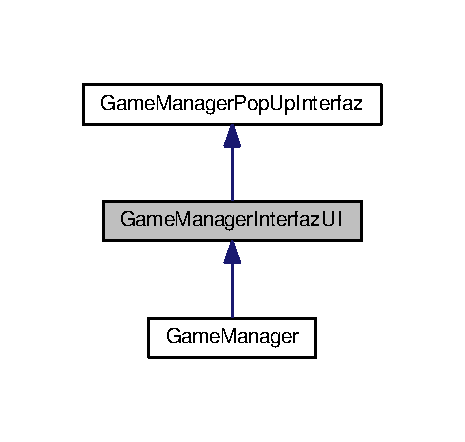
\includegraphics[width=223pt]{class_game_manager_interfaz_u_i__inherit__graph}
\end{center}
\end{figure}


Collaboration diagram for Game\+Manager\+Interfaz\+UI\+:\nopagebreak
\begin{figure}[H]
\begin{center}
\leavevmode
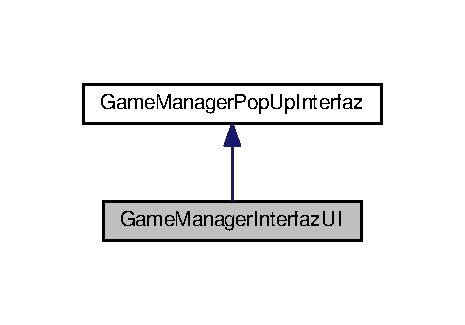
\includegraphics[width=223pt]{class_game_manager_interfaz_u_i__coll__graph}
\end{center}
\end{figure}
\subsection*{Public Member Functions}
\begin{DoxyCompactItemize}
\item 
virtual void \hyperlink{class_game_manager_interfaz_u_i_abc1e55cd9dc327d26ef6fdbfcac05b42}{play} (Galeria\+::\+Code\+Music\+Efecto code\+Music)=0
\item 
virtual void {\bfseries play} (Mix\+\_\+\+Chunk $\ast$p\+Sfx\+Chunk)=0\hypertarget{class_game_manager_interfaz_u_i_aee33c5cc1a5031d8ebe5968b6de9940b}{}\label{class_game_manager_interfaz_u_i_aee33c5cc1a5031d8ebe5968b6de9940b}

\item 
virtual void \hyperlink{class_game_manager_interfaz_u_i_a8ab3930451a7a81829859eb56d72c676}{play\+Sound} (Galeria\+::\+Code\+Music\+Sonido codigo\+Sonido)=0
\item 
virtual void \hyperlink{class_game_manager_interfaz_u_i_a7adf014f12ad93b0a8f569d7d3108bf9}{show\+Pop\+Up} (\hyperlink{class_pop_up_interfaz}{Pop\+Up\+Interfaz} $\ast$pop\+Up\+Interfaz, const int code\+Pop\+Up)=0
\item 
virtual int \hyperlink{class_game_manager_interfaz_u_i_a98ad10caf36808dd0c626a69fa7ffd17}{get\+Active\+Joys} ()=0
\item 
virtual S\+D\+L\+\_\+\+Joystick $\ast$ \hyperlink{class_game_manager_interfaz_u_i_ae0126235dd0099fec45504dc70870032}{get\+Joy} (int i)=0
\item 
virtual \hyperlink{class_l_texture}{L\+Texture} $\ast$ {\bfseries get\+Texture} (Galeria\+::\+Code\+Imagen imagen)=0\hypertarget{class_game_manager_interfaz_u_i_af969f9a01c171fb5c61b1f63c5688003}{}\label{class_game_manager_interfaz_u_i_af969f9a01c171fb5c61b1f63c5688003}

\item 
virtual void \hyperlink{class_game_manager_interfaz_u_i_a9e20a361429abfcc57896fe01955c88e}{cambiar\+Interfaz} (\hyperlink{class_interfaz_u_i}{Interfaz\+UI} $\ast$p\+Interfaz)=0
\item 
virtual void \hyperlink{class_game_manager_interfaz_u_i_aa3ee961c35993d96325520a8176d51f6}{go\+Back} ()=0
\item 
virtual void {\bfseries play\+Sound} (Mix\+\_\+\+Music $\ast$p\+Music, Uint8 volumen)=0\hypertarget{class_game_manager_interfaz_u_i_a8f40ba0bbd33d5dbeee31cfc81aae7cd}{}\label{class_game_manager_interfaz_u_i_a8f40ba0bbd33d5dbeee31cfc81aae7cd}

\item 
virtual void {\bfseries play\+Fade\+In\+Sound} (Mix\+\_\+\+Music $\ast$music, Uint8 volumen)=0\hypertarget{class_game_manager_interfaz_u_i_a8ca83afc38b809b80e9eba8dd9f41ef3}{}\label{class_game_manager_interfaz_u_i_a8ca83afc38b809b80e9eba8dd9f41ef3}

\end{DoxyCompactItemize}


\subsection{Detailed Description}
Esta es la interfaz que debe implemetar un \hyperlink{class_game_manager}{Game\+Manager} si quiere utilizar interfaces. \begin{Desc}
\item[Examples\+: ]\par
\hyperlink{_2home_2manuggz_2_documents_2_projects_2_bomberman_2src_2engine_2interfaces_2_menu_list_label_8hpp-example}{/home/manuggz/\+Documents/\+Projects/\+Bomberman/src/engine/interfaces/\+Menu\+List\+Label.\+hpp}.\end{Desc}


\subsection{Member Function Documentation}
\index{Game\+Manager\+Interfaz\+UI@{Game\+Manager\+Interfaz\+UI}!cambiar\+Interfaz@{cambiar\+Interfaz}}
\index{cambiar\+Interfaz@{cambiar\+Interfaz}!Game\+Manager\+Interfaz\+UI@{Game\+Manager\+Interfaz\+UI}}
\subsubsection[{\texorpdfstring{cambiar\+Interfaz(\+Interfaz\+U\+I $\ast$p\+Interfaz)=0}{cambiarInterfaz(InterfazUI *pInterfaz)=0}}]{\setlength{\rightskip}{0pt plus 5cm}virtual void Game\+Manager\+Interfaz\+U\+I\+::cambiar\+Interfaz (
\begin{DoxyParamCaption}
\item[{{\bf Interfaz\+UI} $\ast$}]{p\+Interfaz}
\end{DoxyParamCaption}
)\hspace{0.3cm}{\ttfamily [pure virtual]}}\hypertarget{class_game_manager_interfaz_u_i_a9e20a361429abfcc57896fe01955c88e}{}\label{class_game_manager_interfaz_u_i_a9e20a361429abfcc57896fe01955c88e}
Cambia la interfaz Actual, por la nueva referenciada. Pausa la Actual y la deja en la pila, si se llama a \hyperlink{class_game_manager_interfaz_u_i_aa3ee961c35993d96325520a8176d51f6}{go\+Back()} se resumirá. 
\begin{DoxyParams}{Parameters}
{\em p\+Juego} & \\
\hline
\end{DoxyParams}


Implemented in \hyperlink{class_game_manager_a1a7ef9efef7dffba5887409b2008f833}{Game\+Manager}.

\index{Game\+Manager\+Interfaz\+UI@{Game\+Manager\+Interfaz\+UI}!get\+Active\+Joys@{get\+Active\+Joys}}
\index{get\+Active\+Joys@{get\+Active\+Joys}!Game\+Manager\+Interfaz\+UI@{Game\+Manager\+Interfaz\+UI}}
\subsubsection[{\texorpdfstring{get\+Active\+Joys()=0}{getActiveJoys()=0}}]{\setlength{\rightskip}{0pt plus 5cm}virtual int Game\+Manager\+Interfaz\+U\+I\+::get\+Active\+Joys (
\begin{DoxyParamCaption}
{}
\end{DoxyParamCaption}
)\hspace{0.3cm}{\ttfamily [pure virtual]}}\hypertarget{class_game_manager_interfaz_u_i_a98ad10caf36808dd0c626a69fa7ffd17}{}\label{class_game_manager_interfaz_u_i_a98ad10caf36808dd0c626a69fa7ffd17}
Obtiene el numero de Joysticks activos \begin{DoxyReturn}{Returns}

\end{DoxyReturn}


Implemented in \hyperlink{class_game_manager_ae47edae1e15eaf1d4624cc4e66a9f559}{Game\+Manager}.

\index{Game\+Manager\+Interfaz\+UI@{Game\+Manager\+Interfaz\+UI}!get\+Joy@{get\+Joy}}
\index{get\+Joy@{get\+Joy}!Game\+Manager\+Interfaz\+UI@{Game\+Manager\+Interfaz\+UI}}
\subsubsection[{\texorpdfstring{get\+Joy(int i)=0}{getJoy(int i)=0}}]{\setlength{\rightskip}{0pt plus 5cm}virtual S\+D\+L\+\_\+\+Joystick$\ast$ Game\+Manager\+Interfaz\+U\+I\+::get\+Joy (
\begin{DoxyParamCaption}
\item[{int}]{i}
\end{DoxyParamCaption}
)\hspace{0.3cm}{\ttfamily [pure virtual]}}\hypertarget{class_game_manager_interfaz_u_i_ae0126235dd0099fec45504dc70870032}{}\label{class_game_manager_interfaz_u_i_ae0126235dd0099fec45504dc70870032}
Obtiene el Joystic en la posición I 
\begin{DoxyParams}{Parameters}
{\em i} & \\
\hline
\end{DoxyParams}
\begin{DoxyReturn}{Returns}

\end{DoxyReturn}


Implemented in \hyperlink{class_game_manager_a9bb21d9af524ae6c72bdd8dc109ce957}{Game\+Manager}.

\index{Game\+Manager\+Interfaz\+UI@{Game\+Manager\+Interfaz\+UI}!go\+Back@{go\+Back}}
\index{go\+Back@{go\+Back}!Game\+Manager\+Interfaz\+UI@{Game\+Manager\+Interfaz\+UI}}
\subsubsection[{\texorpdfstring{go\+Back()=0}{goBack()=0}}]{\setlength{\rightskip}{0pt plus 5cm}virtual void Game\+Manager\+Interfaz\+U\+I\+::go\+Back (
\begin{DoxyParamCaption}
{}
\end{DoxyParamCaption}
)\hspace{0.3cm}{\ttfamily [pure virtual]}}\hypertarget{class_game_manager_interfaz_u_i_aa3ee961c35993d96325520a8176d51f6}{}\label{class_game_manager_interfaz_u_i_aa3ee961c35993d96325520a8176d51f6}
Regresa en la pila de navegación, si no hay nada en la pila se sale del juego. 

Implemented in \hyperlink{class_game_manager_aaa4c8097c4e4288282a261e09ceebcb8}{Game\+Manager}.

\begin{Desc}
\item[Examples\+: ]\par
\hyperlink{_2home_2manuggz_2_documents_2_projects_2_bomberman_2src_2engine_2interfaces_2_menu_list_label_8hpp-example}{/home/manuggz/\+Documents/\+Projects/\+Bomberman/src/engine/interfaces/\+Menu\+List\+Label.\+hpp}.\end{Desc}
\index{Game\+Manager\+Interfaz\+UI@{Game\+Manager\+Interfaz\+UI}!play@{play}}
\index{play@{play}!Game\+Manager\+Interfaz\+UI@{Game\+Manager\+Interfaz\+UI}}
\subsubsection[{\texorpdfstring{play(\+Galeria\+::\+Code\+Music\+Efecto code\+Music)=0}{play(Galeria::CodeMusicEfecto codeMusic)=0}}]{\setlength{\rightskip}{0pt plus 5cm}virtual void Game\+Manager\+Interfaz\+U\+I\+::play (
\begin{DoxyParamCaption}
\item[{Galeria\+::\+Code\+Music\+Efecto}]{code\+Music}
\end{DoxyParamCaption}
)\hspace{0.3cm}{\ttfamily [pure virtual]}}\hypertarget{class_game_manager_interfaz_u_i_abc1e55cd9dc327d26ef6fdbfcac05b42}{}\label{class_game_manager_interfaz_u_i_abc1e55cd9dc327d26ef6fdbfcac05b42}
Reproduce un efecto de sonido 
\begin{DoxyParams}{Parameters}
{\em code\+Music} & \\
\hline
\end{DoxyParams}


Implemented in \hyperlink{class_game_manager_ae693cf42cfb96a0bb6d7de8fad55739d}{Game\+Manager}.

\index{Game\+Manager\+Interfaz\+UI@{Game\+Manager\+Interfaz\+UI}!play\+Sound@{play\+Sound}}
\index{play\+Sound@{play\+Sound}!Game\+Manager\+Interfaz\+UI@{Game\+Manager\+Interfaz\+UI}}
\subsubsection[{\texorpdfstring{play\+Sound(\+Galeria\+::\+Code\+Music\+Sonido codigo\+Sonido)=0}{playSound(Galeria::CodeMusicSonido codigoSonido)=0}}]{\setlength{\rightskip}{0pt plus 5cm}virtual void Game\+Manager\+Interfaz\+U\+I\+::play\+Sound (
\begin{DoxyParamCaption}
\item[{Galeria\+::\+Code\+Music\+Sonido}]{codigo\+Sonido}
\end{DoxyParamCaption}
)\hspace{0.3cm}{\ttfamily [pure virtual]}}\hypertarget{class_game_manager_interfaz_u_i_a8ab3930451a7a81829859eb56d72c676}{}\label{class_game_manager_interfaz_u_i_a8ab3930451a7a81829859eb56d72c676}
Reproduce una musica de fondo 
\begin{DoxyParams}{Parameters}
{\em codigo\+Sonido} & \\
\hline
\end{DoxyParams}


Implemented in \hyperlink{class_game_manager_a55482db663320dd82b11bb221049bd98}{Game\+Manager}.

\index{Game\+Manager\+Interfaz\+UI@{Game\+Manager\+Interfaz\+UI}!show\+Pop\+Up@{show\+Pop\+Up}}
\index{show\+Pop\+Up@{show\+Pop\+Up}!Game\+Manager\+Interfaz\+UI@{Game\+Manager\+Interfaz\+UI}}
\subsubsection[{\texorpdfstring{show\+Pop\+Up(\+Pop\+Up\+Interfaz $\ast$pop\+Up\+Interfaz, const int code\+Pop\+Up)=0}{showPopUp(PopUpInterfaz *popUpInterfaz, const int codePopUp)=0}}]{\setlength{\rightskip}{0pt plus 5cm}virtual void Game\+Manager\+Interfaz\+U\+I\+::show\+Pop\+Up (
\begin{DoxyParamCaption}
\item[{{\bf Pop\+Up\+Interfaz} $\ast$}]{pop\+Up\+Interfaz, }
\item[{const int}]{code\+Pop\+Up}
\end{DoxyParamCaption}
)\hspace{0.3cm}{\ttfamily [pure virtual]}}\hypertarget{class_game_manager_interfaz_u_i_a7adf014f12ad93b0a8f569d7d3108bf9}{}\label{class_game_manager_interfaz_u_i_a7adf014f12ad93b0a8f569d7d3108bf9}
Hace que se muestre un Pop\+Up en la pantalla 
\begin{DoxyParams}{Parameters}
{\em pop\+Up\+Interfaz} & Puntero al Pop\+Up \\
\hline
{\em code\+Pop\+Up} & Codigo que usa el Pop\+Up\\
\hline
\end{DoxyParams}
\begin{DoxyNote}{Note}
Cuando se cierra el Pop\+Up, se pasa el code\+Pop\+Up a la interfaz que esté corriendo 
\end{DoxyNote}


Implemented in \hyperlink{class_game_manager_a79ed8c7a5bdef1baf9290dcab9b55db2}{Game\+Manager}.



The documentation for this class was generated from the following file\+:\begin{DoxyCompactItemize}
\item 
src/engine/interfaces/Game\+Manager\+Interfaz\+U\+I.\+hpp\end{DoxyCompactItemize}

\hypertarget{class_game_manager_pop_up_interfaz}{}\section{Game\+Manager\+Pop\+Up\+Interfaz Class Reference}
\label{class_game_manager_pop_up_interfaz}\index{Game\+Manager\+Pop\+Up\+Interfaz@{Game\+Manager\+Pop\+Up\+Interfaz}}


Inheritance diagram for Game\+Manager\+Pop\+Up\+Interfaz\+:\nopagebreak
\begin{figure}[H]
\begin{center}
\leavevmode
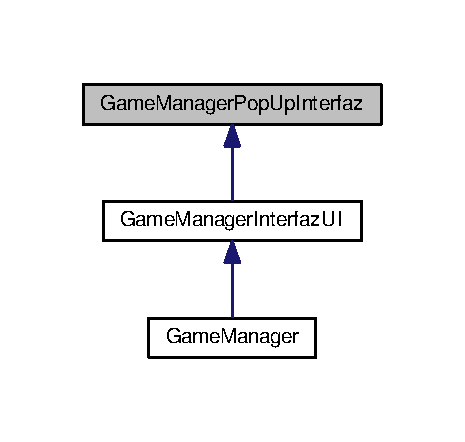
\includegraphics[width=223pt]{class_game_manager_pop_up_interfaz__inherit__graph}
\end{center}
\end{figure}
\subsection*{Public Member Functions}
\begin{DoxyCompactItemize}
\item 
virtual void {\bfseries close\+Pop\+Up} (void $\ast$result=nullptr)=0\hypertarget{class_game_manager_pop_up_interfaz_a2eae4cfc151ef0fbf0a799fd0902fe95}{}\label{class_game_manager_pop_up_interfaz_a2eae4cfc151ef0fbf0a799fd0902fe95}

\item 
virtual S\+D\+L\+\_\+\+Rect {\bfseries get\+Rect\+Screen} ()=0\hypertarget{class_game_manager_pop_up_interfaz_a02a36f94f6986f434d33bae658581b32}{}\label{class_game_manager_pop_up_interfaz_a02a36f94f6986f434d33bae658581b32}

\end{DoxyCompactItemize}


The documentation for this class was generated from the following file\+:\begin{DoxyCompactItemize}
\item 
src/engine/interfaces/Game\+Manager\+Pop\+Up\+Interfaz.\+hpp\end{DoxyCompactItemize}

\hypertarget{class_group}{}\section{Group Class Reference}
\label{class_group}\index{Group@{Group}}


Inheritance diagram for Group\+:\nopagebreak
\begin{figure}[H]
\begin{center}
\leavevmode
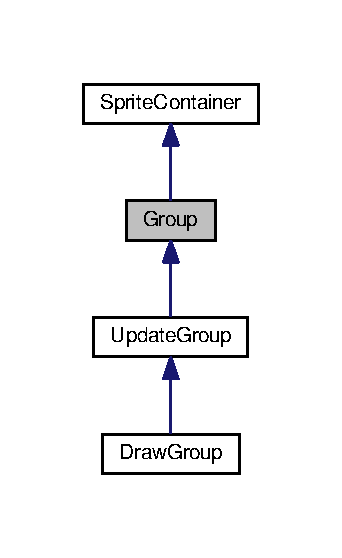
\includegraphics[width=164pt]{class_group__inherit__graph}
\end{center}
\end{figure}


Collaboration diagram for Group\+:\nopagebreak
\begin{figure}[H]
\begin{center}
\leavevmode
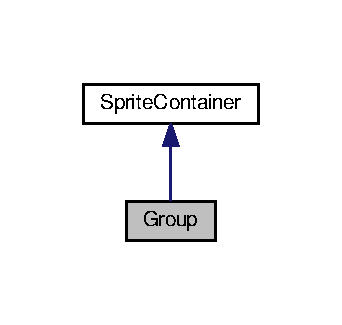
\includegraphics[width=164pt]{class_group__coll__graph}
\end{center}
\end{figure}
\subsection*{Public Member Functions}
\begin{DoxyCompactItemize}
\item 
virtual void {\bfseries add} (\hyperlink{class_sprite}{Sprite} $\ast$)\hypertarget{class_group_a808a26e42fb31af18f1c37584bf3d972}{}\label{class_group_a808a26e42fb31af18f1c37584bf3d972}

\item 
virtual bool {\bfseries erase} (\hyperlink{class_sprite}{Sprite} $\ast$)\hypertarget{class_group_a155ede7c0abf697018b6853adb8ef41e}{}\label{class_group_a155ede7c0abf697018b6853adb8ef41e}

\item 
virtual void {\bfseries clear} ()\hypertarget{class_group_aae18ea1b059afe782eb054409d152d33}{}\label{class_group_aae18ea1b059afe782eb054409d152d33}

\item 
std\+::deque$<$ \hyperlink{class_sprite}{Sprite} $\ast$ $>$ {\bfseries collide} (S\+D\+L\+\_\+\+Rect)\hypertarget{class_group_af4bc12532edc7f9f0233913dec99579e}{}\label{class_group_af4bc12532edc7f9f0233913dec99579e}

\item 
std\+::deque$<$ \hyperlink{class_sprite}{Sprite} $\ast$ $>$ {\bfseries collide} (\hyperlink{class_sprite}{Sprite} $\ast$)\hypertarget{class_group_a13d70b578edcf2d2b93707e84d79c1af}{}\label{class_group_a13d70b578edcf2d2b93707e84d79c1af}

\item 
unsigned long {\bfseries size} ()\hypertarget{class_group_a9ccba97e193d38ab14f99d892860837e}{}\label{class_group_a9ccba97e193d38ab14f99d892860837e}

\item 
deque$<$ \hyperlink{class_sprite}{Sprite} $\ast$ $>$\+::iterator {\bfseries begin} ()\hypertarget{class_group_a58241f01b6efd8e61f8d672595b07b6b}{}\label{class_group_a58241f01b6efd8e61f8d672595b07b6b}

\item 
deque$<$ \hyperlink{class_sprite}{Sprite} $\ast$ $>$\+::iterator {\bfseries end} ()\hypertarget{class_group_a0f7e514ac1a2e8b85d9e25a589374665}{}\label{class_group_a0f7e514ac1a2e8b85d9e25a589374665}

\item 
\hyperlink{class_group_aed00a22ff227ee2657ae44a5cbcedf7c}{$\sim$\+Group} ()
\item 
void {\bfseries kill} ()\hypertarget{class_group_a0b26074a27ca9b4f404d8740743f0cb7}{}\label{class_group_a0b26074a27ca9b4f404d8740743f0cb7}

\end{DoxyCompactItemize}
\subsection*{Protected Member Functions}
\begin{DoxyCompactItemize}
\item 
void \hyperlink{class_group_a876689923759abc572c4b18035400f7c}{erase\+Sprite} (\hyperlink{class_sprite}{Sprite} $\ast$p\+Sprite) override
\end{DoxyCompactItemize}
\subsection*{Protected Attributes}
\begin{DoxyCompactItemize}
\item 
std\+::deque$<$ \hyperlink{class_sprite}{Sprite} $\ast$ $>$ {\bfseries v\+\_\+personajes}\hypertarget{class_group_a22e02baf73646caf87df10bfb70791a7}{}\label{class_group_a22e02baf73646caf87df10bfb70791a7}

\end{DoxyCompactItemize}


\subsection{Constructor \& Destructor Documentation}
\index{Group@{Group}!````~Group@{$\sim$\+Group}}
\index{````~Group@{$\sim$\+Group}!Group@{Group}}
\subsubsection[{\texorpdfstring{$\sim$\+Group()}{~Group()}}]{\setlength{\rightskip}{0pt plus 5cm}Group\+::$\sim$\+Group (
\begin{DoxyParamCaption}
{}
\end{DoxyParamCaption}
)}\hypertarget{class_group_aed00a22ff227ee2657ae44a5cbcedf7c}{}\label{class_group_aed00a22ff227ee2657ae44a5cbcedf7c}
std\+::deque$<$\+Sprite $\ast$$>$ copia = v\+\_\+personajes; 

\subsection{Member Function Documentation}
\index{Group@{Group}!erase\+Sprite@{erase\+Sprite}}
\index{erase\+Sprite@{erase\+Sprite}!Group@{Group}}
\subsubsection[{\texorpdfstring{erase\+Sprite(\+Sprite $\ast$p\+Sprite) override}{eraseSprite(Sprite *pSprite) override}}]{\setlength{\rightskip}{0pt plus 5cm}void Group\+::erase\+Sprite (
\begin{DoxyParamCaption}
\item[{{\bf Sprite} $\ast$}]{p\+Sprite}
\end{DoxyParamCaption}
)\hspace{0.3cm}{\ttfamily [override]}, {\ttfamily [protected]}, {\ttfamily [virtual]}}\hypertarget{class_group_a876689923759abc572c4b18035400f7c}{}\label{class_group_a876689923759abc572c4b18035400f7c}
Función llamada por \hyperlink{class_sprite}{Sprite}, para que solo se elimine él del grupo. 
\begin{DoxyParams}{Parameters}
{\em p\+Sprite} & \\
\hline
\end{DoxyParams}


Implements \hyperlink{class_sprite_container}{Sprite\+Container}.



The documentation for this class was generated from the following files\+:\begin{DoxyCompactItemize}
\item 
src/engine/sprites/C\+Group.\+hpp\item 
src/engine/sprites/C\+Group.\+cpp\end{DoxyCompactItemize}

\hypertarget{struct_t_m_x_1_1_parser_1_1_image}{}\section{T\+MX\+:\+:Parser\+:\+:Image Struct Reference}
\label{struct_t_m_x_1_1_parser_1_1_image}\index{T\+M\+X\+::\+Parser\+::\+Image@{T\+M\+X\+::\+Parser\+::\+Image}}
\subsection*{Public Attributes}
\begin{DoxyCompactItemize}
\item 
std\+::string {\bfseries source}\hypertarget{struct_t_m_x_1_1_parser_1_1_image_acfd86626cd8c040f3a2bfdbdb6d79d20}{}\label{struct_t_m_x_1_1_parser_1_1_image_acfd86626cd8c040f3a2bfdbdb6d79d20}

\item 
std\+::string {\bfseries transparency\+Color}\hypertarget{struct_t_m_x_1_1_parser_1_1_image_a4f7c0ba4c3c7a7525b85370b576a32eb}{}\label{struct_t_m_x_1_1_parser_1_1_image_a4f7c0ba4c3c7a7525b85370b576a32eb}

\end{DoxyCompactItemize}


The documentation for this struct was generated from the following file\+:\begin{DoxyCompactItemize}
\item 
src/engine/mapa/include/T\+M\+X\+Parser.\+h\end{DoxyCompactItemize}

\hypertarget{class_image_component}{}\section{Image\+Component Class Reference}
\label{class_image_component}\index{Image\+Component@{Image\+Component}}


Inheritance diagram for Image\+Component\+:\nopagebreak
\begin{figure}[H]
\begin{center}
\leavevmode
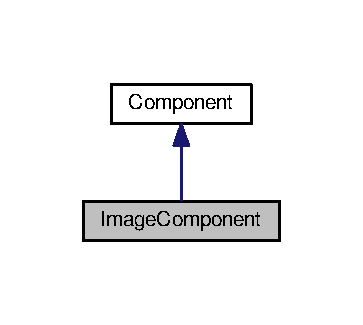
\includegraphics[width=174pt]{class_image_component__inherit__graph}
\end{center}
\end{figure}


Collaboration diagram for Image\+Component\+:\nopagebreak
\begin{figure}[H]
\begin{center}
\leavevmode
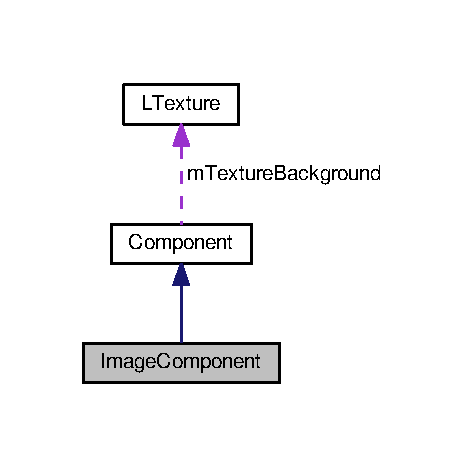
\includegraphics[width=224pt]{class_image_component__coll__graph}
\end{center}
\end{figure}
\subsection*{Public Member Functions}
\begin{DoxyCompactItemize}
\item 
virtual void \hyperlink{class_image_component_a538cae4b9b1f723fa6cb21038387a0f6}{pack} (S\+D\+L\+\_\+\+Renderer $\ast$g\+Renderer) override
\item 
void {\bfseries set\+Image\+Texture} (\hyperlink{class_l_texture}{L\+Texture} $\ast$texture, bool delete\+Anterior=true)\hypertarget{class_image_component_aab7a7fe8608766fa1d6414ce5b4b8281}{}\label{class_image_component_aab7a7fe8608766fa1d6414ce5b4b8281}

\end{DoxyCompactItemize}
\subsection*{Additional Inherited Members}


\subsection{Member Function Documentation}
\index{Image\+Component@{Image\+Component}!pack@{pack}}
\index{pack@{pack}!Image\+Component@{Image\+Component}}
\subsubsection[{\texorpdfstring{pack(\+S\+D\+L\+\_\+\+Renderer $\ast$g\+Renderer) override}{pack(SDL_Renderer *gRenderer) override}}]{\setlength{\rightskip}{0pt plus 5cm}virtual void Image\+Component\+::pack (
\begin{DoxyParamCaption}
\item[{S\+D\+L\+\_\+\+Renderer $\ast$}]{g\+Renderer}
\end{DoxyParamCaption}
)\hspace{0.3cm}{\ttfamily [inline]}, {\ttfamily [override]}, {\ttfamily [virtual]}}\hypertarget{class_image_component_a538cae4b9b1f723fa6cb21038387a0f6}{}\label{class_image_component_a538cae4b9b1f723fa6cb21038387a0f6}
Se encarga de crear las texturas del componente asi como otras acciones asociadas con el renderer Notar que despues de esta funcion se debe llamar a calculate\+Rect, es decir, realizar una nueva calculacion del rectangulo de dibujo del componente 
\begin{DoxyParams}{Parameters}
{\em g\+Renderer} & Render de la pantalla \\
\hline
\end{DoxyParams}


Implements \hyperlink{class_component_aa471f2c3a24525f584ed19cf25222e70}{Component}.



The documentation for this class was generated from the following file\+:\begin{DoxyCompactItemize}
\item 
src/engine/layout/\+Componentes/Image\+Component.\+hpp\end{DoxyCompactItemize}

\hypertarget{struct_t_m_x_1_1_parser_1_1_image_layer}{}\section{T\+MX\+:\+:Parser\+:\+:Image\+Layer Struct Reference}
\label{struct_t_m_x_1_1_parser_1_1_image_layer}\index{T\+M\+X\+::\+Parser\+::\+Image\+Layer@{T\+M\+X\+::\+Parser\+::\+Image\+Layer}}


Collaboration diagram for T\+MX\+:\+:Parser\+:\+:Image\+Layer\+:\nopagebreak
\begin{figure}[H]
\begin{center}
\leavevmode
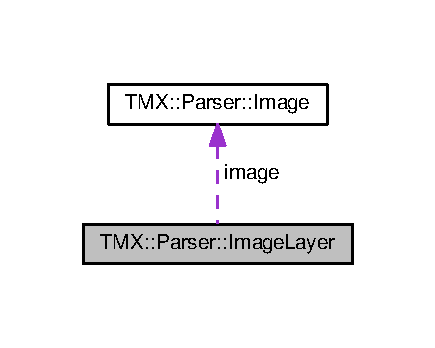
\includegraphics[width=209pt]{struct_t_m_x_1_1_parser_1_1_image_layer__coll__graph}
\end{center}
\end{figure}
\subsection*{Public Attributes}
\begin{DoxyCompactItemize}
\item 
std\+::string {\bfseries name}\hypertarget{struct_t_m_x_1_1_parser_1_1_image_layer_a55c71607f797100313d1da6c6ca21da7}{}\label{struct_t_m_x_1_1_parser_1_1_image_layer_a55c71607f797100313d1da6c6ca21da7}

\item 
float {\bfseries opacity}\hypertarget{struct_t_m_x_1_1_parser_1_1_image_layer_ad368ed956362b077318028f4e443a465}{}\label{struct_t_m_x_1_1_parser_1_1_image_layer_ad368ed956362b077318028f4e443a465}

\item 
bool {\bfseries visible}\hypertarget{struct_t_m_x_1_1_parser_1_1_image_layer_a26c77c9faa5ad39b67eabb43d9b11335}{}\label{struct_t_m_x_1_1_parser_1_1_image_layer_a26c77c9faa5ad39b67eabb43d9b11335}

\item 
std\+::map$<$ std\+::string, std\+::string $>$ {\bfseries property}\hypertarget{struct_t_m_x_1_1_parser_1_1_image_layer_a9e2ed5e998a91e60addc4b750478bd37}{}\label{struct_t_m_x_1_1_parser_1_1_image_layer_a9e2ed5e998a91e60addc4b750478bd37}

\item 
\hyperlink{struct_t_m_x_1_1_parser_1_1_image}{Image} {\bfseries image}\hypertarget{struct_t_m_x_1_1_parser_1_1_image_layer_af6ce802033d9e4bf9a6875ad29193dad}{}\label{struct_t_m_x_1_1_parser_1_1_image_layer_af6ce802033d9e4bf9a6875ad29193dad}

\end{DoxyCompactItemize}


The documentation for this struct was generated from the following file\+:\begin{DoxyCompactItemize}
\item 
src/engine/mapa/include/T\+M\+X\+Parser.\+h\end{DoxyCompactItemize}

\hypertarget{struct_t_m_x_1_1_parser_1_1_image_tile_set}{}\section{T\+MX\+:\+:Parser\+:\+:Image\+Tile\+Set Struct Reference}
\label{struct_t_m_x_1_1_parser_1_1_image_tile_set}\index{T\+M\+X\+::\+Parser\+::\+Image\+Tile\+Set@{T\+M\+X\+::\+Parser\+::\+Image\+Tile\+Set}}
\subsection*{Public Attributes}
\begin{DoxyCompactItemize}
\item 
std\+::string {\bfseries source}\hypertarget{struct_t_m_x_1_1_parser_1_1_image_tile_set_ad2c02e60e229cb43a3c1d61779674daf}{}\label{struct_t_m_x_1_1_parser_1_1_image_tile_set_ad2c02e60e229cb43a3c1d61779674daf}

\item 
unsigned int {\bfseries width}\hypertarget{struct_t_m_x_1_1_parser_1_1_image_tile_set_adebd5ef49162a2386b3717bb2be51944}{}\label{struct_t_m_x_1_1_parser_1_1_image_tile_set_adebd5ef49162a2386b3717bb2be51944}

\item 
unsigned int {\bfseries height}\hypertarget{struct_t_m_x_1_1_parser_1_1_image_tile_set_a5d36d0eb96db7a65044f16be084dfedc}{}\label{struct_t_m_x_1_1_parser_1_1_image_tile_set_a5d36d0eb96db7a65044f16be084dfedc}

\end{DoxyCompactItemize}


The documentation for this struct was generated from the following file\+:\begin{DoxyCompactItemize}
\item 
src/engine/mapa/include/T\+M\+X\+Parser.\+h\end{DoxyCompactItemize}

\hypertarget{class_interfaz_juego}{}\section{Interfaz\+Juego Class Reference}
\label{class_interfaz_juego}\index{Interfaz\+Juego@{Interfaz\+Juego}}


{\ttfamily \#include $<$Interfaz\+Juego.\+hpp$>$}



Inheritance diagram for Interfaz\+Juego\+:\nopagebreak
\begin{figure}[H]
\begin{center}
\leavevmode
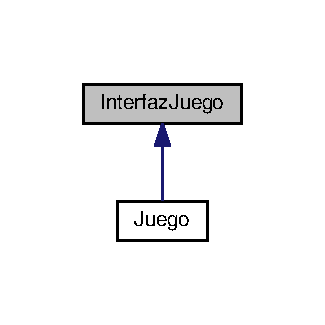
\includegraphics[width=156pt]{class_interfaz_juego__inherit__graph}
\end{center}
\end{figure}
\subsection*{Public Member Functions}
\begin{DoxyCompactItemize}
\item 
virtual \hyperlink{class_l_texture}{L\+Texture} $\ast$ {\bfseries get\+Imagen} (Galeria\+::\+Code\+Imagen code)=0\hypertarget{class_interfaz_juego_ab222b3f39dea890b71acdc3150e66d6d}{}\label{class_interfaz_juego_ab222b3f39dea890b71acdc3150e66d6d}

\item 
virtual S\+D\+L\+\_\+\+Joystick $\ast$ {\bfseries get\+Joy} (int id)=0\hypertarget{class_interfaz_juego_aed1ee6c2c0b68dfb5cdb9a0514bfc1f1}{}\label{class_interfaz_juego_aed1ee6c2c0b68dfb5cdb9a0514bfc1f1}

\item 
virtual int {\bfseries get\+Joys\+Activos} ()=0\hypertarget{class_interfaz_juego_aafadb2ec09cf94823e48e884a609a054}{}\label{class_interfaz_juego_aafadb2ec09cf94823e48e884a609a054}

\item 
virtual Nivel\+Mapa\+::\+Extremo\+Colision {\bfseries colision\+Con\+Mapa} (S\+D\+L\+\_\+\+Rect rect\+\_\+coli, int $\ast$lado\+\_\+colision=nullptr, bool solo\+Bloques\+No\+Traspasables=false)=0\hypertarget{class_interfaz_juego_ab744f7c22be984491e63dcbd5b05c556}{}\label{class_interfaz_juego_ab744f7c22be984491e63dcbd5b05c556}

\item 
virtual deque$<$ \hyperlink{class_sprite}{Sprite} $\ast$ $>$ {\bfseries colision\+Con\+Bombas} (S\+D\+L\+\_\+\+Rect rect)=0\hypertarget{class_interfaz_juego_a78f25518403ce658e93e528dc99ac5b9}{}\label{class_interfaz_juego_a78f25518403ce658e93e528dc99ac5b9}

\item 
virtual deque$<$ \hyperlink{class_sprite}{Sprite} $\ast$ $>$ {\bfseries colision\+Bloque\+En\+Llamas} (S\+D\+L\+\_\+\+Rect rect)=0\hypertarget{class_interfaz_juego_a4d3aa11daa5f3e98d7f3cfe4cb00b636}{}\label{class_interfaz_juego_a4d3aa11daa5f3e98d7f3cfe4cb00b636}

\item 
virtual deque$<$ \hyperlink{class_sprite}{Sprite} $\ast$ $>$ {\bfseries colision\+Con\+Items} (S\+D\+L\+\_\+\+Rect rect)=0\hypertarget{class_interfaz_juego_abb32e88a7358328dc66bdcf1538976bc}{}\label{class_interfaz_juego_abb32e88a7358328dc66bdcf1538976bc}

\item 
virtual deque$<$ \hyperlink{class_sprite}{Sprite} $\ast$ $>$ {\bfseries colision\+Con\+Explosiones} (S\+D\+L\+\_\+\+Rect rect)=0\hypertarget{class_interfaz_juego_adf29f16f79645436c70efef98b522608}{}\label{class_interfaz_juego_adf29f16f79645436c70efef98b522608}

\item 
virtual bool {\bfseries is\+Out\+Of\+Map\+Bounds} (S\+D\+L\+\_\+\+Rect rect)=0\hypertarget{class_interfaz_juego_a4a7543a340f74cff355aa900329f5c89}{}\label{class_interfaz_juego_a4a7543a340f74cff355aa900329f5c89}

\item 
virtual \hyperlink{class_bomba}{Bomba} $\ast$ {\bfseries agregar\+Bomba} (\hyperlink{class_player}{Player} $\ast$player\+Propietario)=0\hypertarget{class_interfaz_juego_a51f9c4d2cbb8d897bae5f201e5e800c1}{}\label{class_interfaz_juego_a51f9c4d2cbb8d897bae5f201e5e800c1}

\item 
virtual \hyperlink{class_tile_en_llamas}{Tile\+En\+Llamas} $\ast$ {\bfseries agregar\+Bloque\+En\+Llamas} (int x, int y)=0\hypertarget{class_interfaz_juego_a9acf8fb9f782d448043535d553fb7535}{}\label{class_interfaz_juego_a9acf8fb9f782d448043535d553fb7535}

\item 
virtual bool {\bfseries es\+Bloque\+Solido} (int x, int y)=0\hypertarget{class_interfaz_juego_ac4c1573e92f587b81843e7cab25e2581}{}\label{class_interfaz_juego_ac4c1573e92f587b81843e7cab25e2581}

\item 
virtual bool {\bfseries es\+Bloque\+Rompible} (int x, int y)=0\hypertarget{class_interfaz_juego_a3fb994485276a791e67e7d4290c1ea34}{}\label{class_interfaz_juego_a3fb994485276a791e67e7d4290c1ea34}

\item 
virtual void {\bfseries player\+Muerto} (\hyperlink{class_player}{Player} $\ast$p\+Player, \hyperlink{class_sprite}{Sprite} $\ast$p\+Player\+Causante)=0\hypertarget{class_interfaz_juego_a8a696b1e5b7998e786e3537788f4c9a6}{}\label{class_interfaz_juego_a8a696b1e5b7998e786e3537788f4c9a6}

\end{DoxyCompactItemize}


\subsection{Detailed Description}
Esta clase contiene las funciones que un 

The documentation for this class was generated from the following file\+:\begin{DoxyCompactItemize}
\item 
src/\+Interfaces/juego/\hyperlink{_interfaz_juego_8hpp}{Interfaz\+Juego.\+hpp}\end{DoxyCompactItemize}

\hypertarget{class_interfaz_juego_othello}{}\section{Interfaz\+Juego\+Othello Class Reference}
\label{class_interfaz_juego_othello}\index{Interfaz\+Juego\+Othello@{Interfaz\+Juego\+Othello}}


Inheritance diagram for Interfaz\+Juego\+Othello\+:
\nopagebreak
\begin{figure}[H]
\begin{center}
\leavevmode
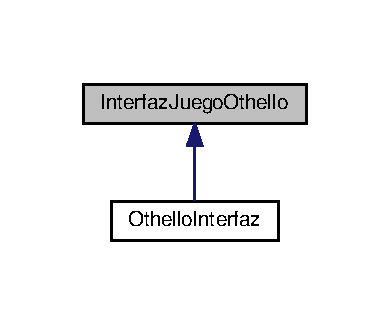
\includegraphics[width=187pt]{class_interfaz_juego_othello__inherit__graph}
\end{center}
\end{figure}
\subsection*{Public Member Functions}
\begin{DoxyCompactItemize}
\item 
virtual void {\bfseries play\+Sfx} (Mix\+\_\+\+Chunk $\ast$p\+Sfx\+Chunk)=0\hypertarget{class_interfaz_juego_othello_ac76194183988304d072f51f7a012de6a}{}\label{class_interfaz_juego_othello_ac76194183988304d072f51f7a012de6a}

\item 
virtual void {\bfseries seleccionada\+Posicion\+Invalida} (int turno\+Actual)=0\hypertarget{class_interfaz_juego_othello_a4a1d8cb6abc160c2d6ed853678f680b4}{}\label{class_interfaz_juego_othello_a4a1d8cb6abc160c2d6ed853678f680b4}

\item 
virtual void {\bfseries cambiado\+Turno} (int turno\+Actual, int n\+Volteadas\+Turno\+Anterior)=0\hypertarget{class_interfaz_juego_othello_a8fd097ef782d8151a3d27d396e98174d}{}\label{class_interfaz_juego_othello_a8fd097ef782d8151a3d27d396e98174d}

\item 
virtual void {\bfseries cambio\+Estado\+Tablero} (int n\+Blancas, int n\+Negras)=0\hypertarget{class_interfaz_juego_othello_aecf123771836b60b83839523770ef163}{}\label{class_interfaz_juego_othello_aecf123771836b60b83839523770ef163}

\item 
virtual void {\bfseries se\+Acabo\+El\+Juego} (int n\+Blancas, int n\+Negras)=0\hypertarget{class_interfaz_juego_othello_a54efd75197e1def2a8f70f35ba7b970e}{}\label{class_interfaz_juego_othello_a54efd75197e1def2a8f70f35ba7b970e}

\end{DoxyCompactItemize}


The documentation for this class was generated from the following file\+:\begin{DoxyCompactItemize}
\item 
src/testsotrosjuegos/\+Othello/Othello\+Juego.\+hpp\end{DoxyCompactItemize}

\hypertarget{class_interfaz_juego_tetris}{}\section{Interfaz\+Juego\+Tetris Class Reference}
\label{class_interfaz_juego_tetris}\index{Interfaz\+Juego\+Tetris@{Interfaz\+Juego\+Tetris}}


Inheritance diagram for Interfaz\+Juego\+Tetris\+:
\nopagebreak
\begin{figure}[H]
\begin{center}
\leavevmode
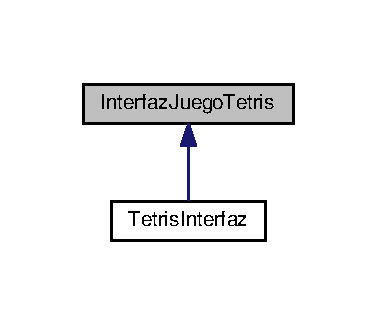
\includegraphics[width=181pt]{class_interfaz_juego_tetris__inherit__graph}
\end{center}
\end{figure}
\subsection*{Public Member Functions}
\begin{DoxyCompactItemize}
\item 
virtual void {\bfseries nuevo\+Tetromino\+Siguiente} (\hyperlink{class_tetromino}{Tetromino} $\ast$nuevo\+Tetromino\+Siguiente)=0\hypertarget{class_interfaz_juego_tetris_a9b27aa0041ec81b9c4dda8539fe21385}{}\label{class_interfaz_juego_tetris_a9b27aa0041ec81b9c4dda8539fe21385}

\item 
virtual void {\bfseries tetris\+Retry} (int tetris\+ID)=0\hypertarget{class_interfaz_juego_tetris_a8fd933b642725742a4f5d9b035e0f8ec}{}\label{class_interfaz_juego_tetris_a8fd933b642725742a4f5d9b035e0f8ec}

\item 
virtual void {\bfseries tetris\+End} (int tetris\+ID)=0\hypertarget{class_interfaz_juego_tetris_aee4fc00412f8d4dfffd5f580ab8e0817}{}\label{class_interfaz_juego_tetris_aee4fc00412f8d4dfffd5f580ab8e0817}

\item 
virtual void {\bfseries tetris\+Lineas\+Completadas} (int tetris\+ID, int n\+Lineas)=0\hypertarget{class_interfaz_juego_tetris_a9e11a199a7615f034d8be30eeedc6f68}{}\label{class_interfaz_juego_tetris_a9e11a199a7615f034d8be30eeedc6f68}

\item 
virtual void {\bfseries tetris\+Paused} (int tetris\+ID)=0\hypertarget{class_interfaz_juego_tetris_ad5370760fceffca5e71a9ed651baf9d5}{}\label{class_interfaz_juego_tetris_ad5370760fceffca5e71a9ed651baf9d5}

\item 
virtual void {\bfseries tetris\+Resumed} (int tetris\+ID)=0\hypertarget{class_interfaz_juego_tetris_a45260ee6da54129577ea96795f506444}{}\label{class_interfaz_juego_tetris_a45260ee6da54129577ea96795f506444}

\item 
virtual void {\bfseries tetris\+Game\+Over} (int tetris\+ID)=0\hypertarget{class_interfaz_juego_tetris_aa2ceb116d7d8be58bc924ea2e96602d4}{}\label{class_interfaz_juego_tetris_aa2ceb116d7d8be58bc924ea2e96602d4}

\item 
virtual void {\bfseries play\+Sfx} (Mix\+\_\+\+Chunk $\ast$p\+Sfx\+Chunk)=0\hypertarget{class_interfaz_juego_tetris_a34572732b0e83f406322e268e3776906}{}\label{class_interfaz_juego_tetris_a34572732b0e83f406322e268e3776906}

\item 
virtual void {\bfseries tetris\+Hard\+Drop} (int tetris\+ID, int n\+Cells)=0\hypertarget{class_interfaz_juego_tetris_a68d6072ed1da605ee7e9bedddd74aaec}{}\label{class_interfaz_juego_tetris_a68d6072ed1da605ee7e9bedddd74aaec}

\item 
virtual void {\bfseries tetris\+Soft\+Drop} (int tetris\+ID, int n\+Cells)=0\hypertarget{class_interfaz_juego_tetris_a6519b3f35542a3df94379719def0b9ce}{}\label{class_interfaz_juego_tetris_a6519b3f35542a3df94379719def0b9ce}

\end{DoxyCompactItemize}


The documentation for this class was generated from the following file\+:\begin{DoxyCompactItemize}
\item 
src/testsotrosjuegos/\+Tetris/Tetris\+Juego.\+hpp\end{DoxyCompactItemize}

\hypertarget{class_interfaz_sprite_group}{}\section{Interfaz\+Sprite\+Group Class Reference}
\label{class_interfaz_sprite_group}\index{Interfaz\+Sprite\+Group@{Interfaz\+Sprite\+Group}}


Inheritance diagram for Interfaz\+Sprite\+Group\+:
\nopagebreak
\begin{figure}[H]
\begin{center}
\leavevmode
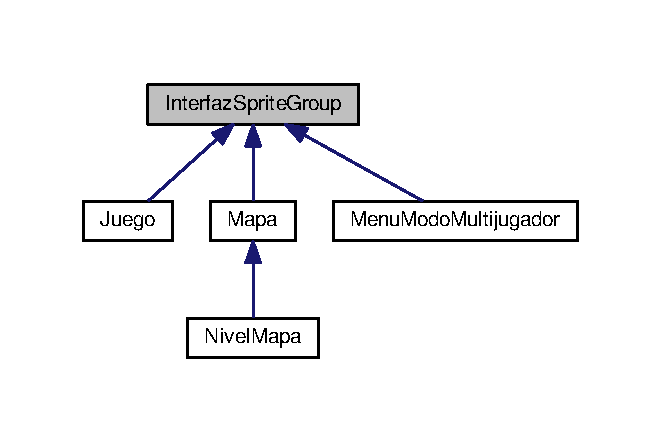
\includegraphics[width=317pt]{class_interfaz_sprite_group__inherit__graph}
\end{center}
\end{figure}
\subsection*{Public Member Functions}
\begin{DoxyCompactItemize}
\item 
virtual void \hyperlink{class_interfaz_sprite_group_acad50741e8bab94e3ce1f8c4c0cbad52}{eliminar\+Sprite} (\hyperlink{class_sprite}{Sprite} $\ast$)=0
\end{DoxyCompactItemize}


\subsection{Member Function Documentation}
\index{Interfaz\+Sprite\+Group@{Interfaz\+Sprite\+Group}!eliminar\+Sprite@{eliminar\+Sprite}}
\index{eliminar\+Sprite@{eliminar\+Sprite}!Interfaz\+Sprite\+Group@{Interfaz\+Sprite\+Group}}
\subsubsection[{\texorpdfstring{eliminar\+Sprite(\+Sprite $\ast$)=0}{eliminarSprite(Sprite *)=0}}]{\setlength{\rightskip}{0pt plus 5cm}virtual void Interfaz\+Sprite\+Group\+::eliminar\+Sprite (
\begin{DoxyParamCaption}
\item[{{\bf Sprite} $\ast$}]{}
\end{DoxyParamCaption}
)\hspace{0.3cm}{\ttfamily [pure virtual]}}\hypertarget{class_interfaz_sprite_group_acad50741e8bab94e3ce1f8c4c0cbad52}{}\label{class_interfaz_sprite_group_acad50741e8bab94e3ce1f8c4c0cbad52}
Elimina un \hyperlink{class_sprite}{Sprite} de Memoria. Esta función es llamada desde un Update\+Group/\+Derivado cuando se elimina un \hyperlink{class_sprite}{Sprite} con kill(). 

Implemented in \hyperlink{class_menu_modo_multijugador_a0957d2b62ca4851a3a868403767c9d61}{Menu\+Modo\+Multijugador}, \hyperlink{class_juego_acaae61b971f3c2b767925db38da41d5c}{Juego}, and \hyperlink{class_mapa_a142d3bbb3a2166aa575b90e50c790a36}{Mapa}.



The documentation for this class was generated from the following file\+:\begin{DoxyCompactItemize}
\item 
src/engine/interfaces/Interfaz\+Sprite\+Group.\+hpp\end{DoxyCompactItemize}

\hypertarget{class_interfaz_u_i}{}\section{Interfaz\+UI Class Reference}
\label{class_interfaz_u_i}\index{Interfaz\+UI@{Interfaz\+UI}}


{\ttfamily \#include $<$Interfaz\+U\+I.\+hpp$>$}



Inheritance diagram for Interfaz\+UI\+:
\nopagebreak
\begin{figure}[H]
\begin{center}
\leavevmode
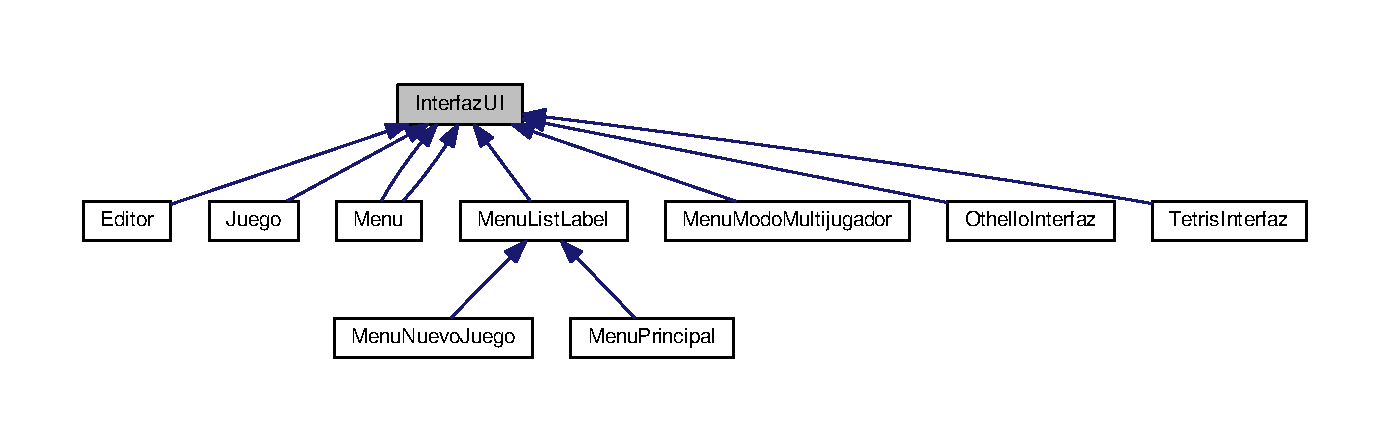
\includegraphics[width=350pt]{class_interfaz_u_i__inherit__graph}
\end{center}
\end{figure}


Collaboration diagram for Interfaz\+UI\+:\nopagebreak
\begin{figure}[H]
\begin{center}
\leavevmode
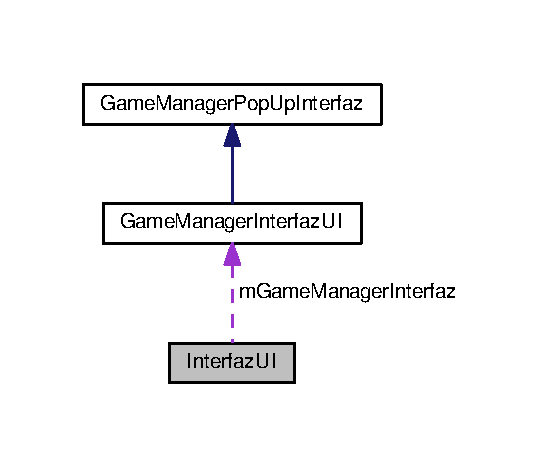
\includegraphics[width=261pt]{class_interfaz_u_i__coll__graph}
\end{center}
\end{figure}
\subsection*{Public Member Functions}
\begin{DoxyCompactItemize}
\item 
\hyperlink{class_interfaz_u_i_aa6578b54c6ff801c9757ea6b9fdfba18}{Interfaz\+UI} (\hyperlink{class_game_manager_interfaz_u_i}{Game\+Manager\+Interfaz\+UI} $\ast$game\+Manager\+Interfaz)
\item 
virtual void \hyperlink{class_interfaz_u_i_a312ba3176f7778589cd67f1828682012}{prepare} ()
\item 
virtual void \hyperlink{class_interfaz_u_i_a9dd59265e0790f06862fdfb12494767e}{create\+UI} (S\+D\+L\+\_\+\+Renderer $\ast$g\+Renderer)
\item 
virtual void \hyperlink{class_interfaz_u_i_a2a80214a4387c21c34a617a8a96996ca}{start} ()
\item 
virtual bool \hyperlink{class_interfaz_u_i_aa733a6aaaafc47daabae6a3156b97e18}{is\+Paused} ()
\item 
virtual bool \hyperlink{class_interfaz_u_i_a46a55209d8216f9afcc52313aacd6083}{is\+Started} ()
\item 
virtual bool \hyperlink{class_interfaz_u_i_a6514cf3d3d8c8d3faf01ee917ab0d4c1}{is\+Stopped} ()
\item 
virtual void {\bfseries pause} ()\hypertarget{class_interfaz_u_i_a1f20c514d5b0fd3965d5a1beb737f14c}{}\label{class_interfaz_u_i_a1f20c514d5b0fd3965d5a1beb737f14c}

\item 
virtual void {\bfseries stop} ()\hypertarget{class_interfaz_u_i_a64b64ee8944584ffbb3e478ab91ab280}{}\label{class_interfaz_u_i_a64b64ee8944584ffbb3e478ab91ab280}

\item 
virtual void {\bfseries resume} ()\hypertarget{class_interfaz_u_i_a9aaf3c1c5e7b46e791db0939deaaf15c}{}\label{class_interfaz_u_i_a9aaf3c1c5e7b46e791db0939deaaf15c}

\item 
virtual void {\bfseries procesar\+Evento} (S\+D\+L\+\_\+\+Event $\ast$event)\hypertarget{class_interfaz_u_i_adda39beb91f3089dd32d66ff2a5cea23}{}\label{class_interfaz_u_i_adda39beb91f3089dd32d66ff2a5cea23}

\item 
virtual void {\bfseries update} ()\hypertarget{class_interfaz_u_i_aac531d5813cbf9d7595c8c908ab3fbbc}{}\label{class_interfaz_u_i_aac531d5813cbf9d7595c8c908ab3fbbc}

\item 
virtual void {\bfseries update\+When\+Pop\+Up} ()\hypertarget{class_interfaz_u_i_ac1bb29ecec25c6087fbbcf31f8b800b7}{}\label{class_interfaz_u_i_ac1bb29ecec25c6087fbbcf31f8b800b7}

\item 
virtual void {\bfseries result\+Pop\+Up} (void $\ast$result, int i)\hypertarget{class_interfaz_u_i_a3ced38e69975a52d3754e9d162f36a2a}{}\label{class_interfaz_u_i_a3ced38e69975a52d3754e9d162f36a2a}

\item 
virtual void {\bfseries draw} (S\+D\+L\+\_\+\+Renderer $\ast$g\+Renderer)=0\hypertarget{class_interfaz_u_i_ae5be2033f8219024253243d38f570a64}{}\label{class_interfaz_u_i_ae5be2033f8219024253243d38f570a64}

\end{DoxyCompactItemize}
\subsection*{Protected Attributes}
\begin{DoxyCompactItemize}
\item 
\hyperlink{class_game_manager_interfaz_u_i}{Game\+Manager\+Interfaz\+UI} $\ast$ {\bfseries m\+Game\+Manager\+Interfaz}\hypertarget{class_interfaz_u_i_adf577e23c777efaf6e9323f8f3ac847a}{}\label{class_interfaz_u_i_adf577e23c777efaf6e9323f8f3ac847a}

\item 
bool {\bfseries m\+Is\+Paused} = false\hypertarget{class_interfaz_u_i_a060ab00c29297fc4e34395d731c5415e}{}\label{class_interfaz_u_i_a060ab00c29297fc4e34395d731c5415e}

\item 
bool {\bfseries m\+Is\+Started} = false\hypertarget{class_interfaz_u_i_aa5920e1cb002b0a09380841149ec6b84}{}\label{class_interfaz_u_i_aa5920e1cb002b0a09380841149ec6b84}

\item 
bool {\bfseries m\+Is\+Stopped} = false\hypertarget{class_interfaz_u_i_a067e003fadf4e356b9533d15138566f7}{}\label{class_interfaz_u_i_a067e003fadf4e356b9533d15138566f7}

\end{DoxyCompactItemize}


\subsection{Detailed Description}
Clase base para todas las interfaces mostradas al usuario. Maneja estados como Pausado/\+Comenzado.

Los metodos son llamados por el \hyperlink{class_game_manager}{Game\+Manager}, algunos siguen un Orden.

El Orden de llamada desde el \hyperlink{class_game_manager}{Game\+Manager} es\+:

\hyperlink{class_interfaz_u_i_a312ba3176f7778589cd67f1828682012}{prepare()} \hyperlink{class_interfaz_u_i_a9dd59265e0790f06862fdfb12494767e}{create\+U\+I()} \hyperlink{class_interfaz_u_i_a2a80214a4387c21c34a617a8a96996ca}{start()}

Cuando un Pop\+Up se va a mostrar o se agrega una interfaz al stack se llama a pause().

Cuando se establece un root en el GM o se hace back en el GM se llama a stop. \begin{Desc}
\item[Examples\+: ]\par
\hyperlink{_2home_2manuggz_2_documents_2_projects_2_bomberman_2src_2engine_2interfaces_2_menu_list_label_8hpp-example}{/home/manuggz/\+Documents/\+Projects/\+Bomberman/src/engine/interfaces/\+Menu\+List\+Label.\+hpp}.\end{Desc}


\subsection{Constructor \& Destructor Documentation}
\index{Interfaz\+UI@{Interfaz\+UI}!Interfaz\+UI@{Interfaz\+UI}}
\index{Interfaz\+UI@{Interfaz\+UI}!Interfaz\+UI@{Interfaz\+UI}}
\subsubsection[{\texorpdfstring{Interfaz\+U\+I(\+Game\+Manager\+Interfaz\+U\+I $\ast$game\+Manager\+Interfaz)}{InterfazUI(GameManagerInterfazUI *gameManagerInterfaz)}}]{\setlength{\rightskip}{0pt plus 5cm}Interfaz\+U\+I\+::\+Interfaz\+UI (
\begin{DoxyParamCaption}
\item[{{\bf Game\+Manager\+Interfaz\+UI} $\ast$}]{game\+Manager\+Interfaz}
\end{DoxyParamCaption}
)\hspace{0.3cm}{\ttfamily [inline]}}\hypertarget{class_interfaz_u_i_aa6578b54c6ff801c9757ea6b9fdfba18}{}\label{class_interfaz_u_i_aa6578b54c6ff801c9757ea6b9fdfba18}
Establece una referencia a un \hyperlink{class_game_manager}{Game\+Manager}. 
\begin{DoxyParams}{Parameters}
{\em game\+Manager\+Interfaz} & Instancia de un \hyperlink{class_game_manager}{Game\+Manager} que implemente la interfaz requerida \\
\hline
\end{DoxyParams}
\begin{Desc}
\item[Examples\+: ]\par
\hyperlink{_2home_2manuggz_2_documents_2_projects_2_bomberman_2src_2engine_2interfaces_2_menu_list_label_8hpp-example}{/home/manuggz/\+Documents/\+Projects/\+Bomberman/src/engine/interfaces/\+Menu\+List\+Label.\+hpp}.\end{Desc}


\subsection{Member Function Documentation}
\index{Interfaz\+UI@{Interfaz\+UI}!create\+UI@{create\+UI}}
\index{create\+UI@{create\+UI}!Interfaz\+UI@{Interfaz\+UI}}
\subsubsection[{\texorpdfstring{create\+U\+I(\+S\+D\+L\+\_\+\+Renderer $\ast$g\+Renderer)}{createUI(SDL_Renderer *gRenderer)}}]{\setlength{\rightskip}{0pt plus 5cm}virtual void Interfaz\+U\+I\+::create\+UI (
\begin{DoxyParamCaption}
\item[{S\+D\+L\+\_\+\+Renderer $\ast$}]{g\+Renderer}
\end{DoxyParamCaption}
)\hspace{0.3cm}{\ttfamily [inline]}, {\ttfamily [virtual]}}\hypertarget{class_interfaz_u_i_a9dd59265e0790f06862fdfb12494767e}{}\label{class_interfaz_u_i_a9dd59265e0790f06862fdfb12494767e}
Este metodo se encarga de crear la UI necesaria/inicial de la interfaz. En algunos juegos no es necesario establecer UI en este metodo, sino dibujarlo tod cuando se llama a Interfaz\+U\+I\+::draw

Sin embargo, crear los elementos de la UI por adelantado ayuda en la utilización de dirty rects y parecidos. 
\begin{DoxyParams}{Parameters}
{\em g\+Renderer} & \\
\hline
\end{DoxyParams}


Reimplemented in \hyperlink{class_tetris_interfaz_a31071ba2d473bfc4cd600f9d4cac2e11}{Tetris\+Interfaz}, \hyperlink{class_menu_list_label_aa4622ae2bc0bf7d31aa8fe8483103e27}{Menu\+List\+Label}, \hyperlink{class_othello_interfaz_af54c0303476eca871b509d6b77151abe}{Othello\+Interfaz}, \hyperlink{class_menu_modo_multijugador_aa87c06427be64fd73e17d9ea37d8744e}{Menu\+Modo\+Multijugador}, \hyperlink{class_juego_a8dd19e6a53b446292e3e15e5e164ed05}{Juego}, \hyperlink{class_menu_a71c36f40cdf039d07172222f4e1c4566}{Menu}, and \hyperlink{class_menu_a71c36f40cdf039d07172222f4e1c4566}{Menu}.

\index{Interfaz\+UI@{Interfaz\+UI}!is\+Paused@{is\+Paused}}
\index{is\+Paused@{is\+Paused}!Interfaz\+UI@{Interfaz\+UI}}
\subsubsection[{\texorpdfstring{is\+Paused()}{isPaused()}}]{\setlength{\rightskip}{0pt plus 5cm}virtual bool Interfaz\+U\+I\+::is\+Paused (
\begin{DoxyParamCaption}
{}
\end{DoxyParamCaption}
)\hspace{0.3cm}{\ttfamily [inline]}, {\ttfamily [virtual]}}\hypertarget{class_interfaz_u_i_aa733a6aaaafc47daabae6a3156b97e18}{}\label{class_interfaz_u_i_aa733a6aaaafc47daabae6a3156b97e18}
Dice si la interfaz está pausada. Lo cual puede suceder debido a que se está mostrando un Pop\+Up al usuario, o que hay otra interfaz en el top de la pila. \begin{DoxyReturn}{Returns}

\end{DoxyReturn}
\index{Interfaz\+UI@{Interfaz\+UI}!is\+Started@{is\+Started}}
\index{is\+Started@{is\+Started}!Interfaz\+UI@{Interfaz\+UI}}
\subsubsection[{\texorpdfstring{is\+Started()}{isStarted()}}]{\setlength{\rightskip}{0pt plus 5cm}virtual bool Interfaz\+U\+I\+::is\+Started (
\begin{DoxyParamCaption}
{}
\end{DoxyParamCaption}
)\hspace{0.3cm}{\ttfamily [inline]}, {\ttfamily [virtual]}}\hypertarget{class_interfaz_u_i_a46a55209d8216f9afcc52313aacd6083}{}\label{class_interfaz_u_i_a46a55209d8216f9afcc52313aacd6083}
Dice si se ha iniciado la interfaz. Una interfaz se considera iniciada si ejecuta \hyperlink{class_interfaz_u_i_a312ba3176f7778589cd67f1828682012}{prepare()}-\/$>$\hyperlink{class_interfaz_u_i_a9dd59265e0790f06862fdfb12494767e}{create\+U\+I()}-\/$>$\hyperlink{class_interfaz_u_i_a2a80214a4387c21c34a617a8a96996ca}{start()} \begin{DoxyReturn}{Returns}

\end{DoxyReturn}
\index{Interfaz\+UI@{Interfaz\+UI}!is\+Stopped@{is\+Stopped}}
\index{is\+Stopped@{is\+Stopped}!Interfaz\+UI@{Interfaz\+UI}}
\subsubsection[{\texorpdfstring{is\+Stopped()}{isStopped()}}]{\setlength{\rightskip}{0pt plus 5cm}virtual bool Interfaz\+U\+I\+::is\+Stopped (
\begin{DoxyParamCaption}
{}
\end{DoxyParamCaption}
)\hspace{0.3cm}{\ttfamily [inline]}, {\ttfamily [virtual]}}\hypertarget{class_interfaz_u_i_a6514cf3d3d8c8d3faf01ee917ab0d4c1}{}\label{class_interfaz_u_i_a6514cf3d3d8c8d3faf01ee917ab0d4c1}
Dice si la interfaz está detenida. Una vez que la interfaz está detenida no se vuelve a ejecutar. Cuando el GM detecta una interfaz detenida la elimina. \begin{DoxyReturn}{Returns}

\end{DoxyReturn}
\index{Interfaz\+UI@{Interfaz\+UI}!prepare@{prepare}}
\index{prepare@{prepare}!Interfaz\+UI@{Interfaz\+UI}}
\subsubsection[{\texorpdfstring{prepare()}{prepare()}}]{\setlength{\rightskip}{0pt plus 5cm}virtual void Interfaz\+U\+I\+::prepare (
\begin{DoxyParamCaption}
{}
\end{DoxyParamCaption}
)\hspace{0.3cm}{\ttfamily [inline]}, {\ttfamily [virtual]}}\hypertarget{class_interfaz_u_i_a312ba3176f7778589cd67f1828682012}{}\label{class_interfaz_u_i_a312ba3176f7778589cd67f1828682012}
Se encarga de establecer valores de variables iniciales de la Interfaz Este metodo se ejecuta antes de create\+UI, por lo que puede usarse para obtener datos necesarios para la creacion de la UI 

Reimplemented in \hyperlink{class_menu_list_label_aaa91bf445c3db2fa2008a06b5e96df24}{Menu\+List\+Label}, \hyperlink{class_tetris_interfaz_abc98e6a4974e89f5dd40177439c07d54}{Tetris\+Interfaz}, \hyperlink{class_menu_modo_multijugador_a422baa9893784cacd414b13fbd34e7d2}{Menu\+Modo\+Multijugador}, \hyperlink{class_juego_a5db4a2c61a5853c6a02341d0b9e77cbb}{Juego}, \hyperlink{class_othello_interfaz_ab090b9f23617c40327b0ea0f0bd7cd6e}{Othello\+Interfaz}, \hyperlink{class_menu_a12119ab1b9abbc5215f6b80be4e3f94b}{Menu}, and \hyperlink{class_menu_a12119ab1b9abbc5215f6b80be4e3f94b}{Menu}.

\begin{Desc}
\item[Examples\+: ]\par
\hyperlink{_2home_2manuggz_2_documents_2_projects_2_bomberman_2src_2engine_2interfaces_2_menu_list_label_8hpp-example}{/home/manuggz/\+Documents/\+Projects/\+Bomberman/src/engine/interfaces/\+Menu\+List\+Label.\+hpp}.\end{Desc}
\index{Interfaz\+UI@{Interfaz\+UI}!start@{start}}
\index{start@{start}!Interfaz\+UI@{Interfaz\+UI}}
\subsubsection[{\texorpdfstring{start()}{start()}}]{\setlength{\rightskip}{0pt plus 5cm}virtual void Interfaz\+U\+I\+::start (
\begin{DoxyParamCaption}
{}
\end{DoxyParamCaption}
)\hspace{0.3cm}{\ttfamily [inline]}, {\ttfamily [virtual]}}\hypertarget{class_interfaz_u_i_a2a80214a4387c21c34a617a8a96996ca}{}\label{class_interfaz_u_i_a2a80214a4387c21c34a617a8a96996ca}
Este metodo se encarga de Iniciar la Interfaz, al igual que los anteriores métodos. Este metodo debe usarse para dividir el inicio de variables y elementos del juego. 

Reimplemented in \hyperlink{class_tetris_interfaz_a9a600a6aab6f3d92b1792e35d3ae4897}{Tetris\+Interfaz}, \hyperlink{class_menu_ae3d38e9e9b2bfc6a99810fbd178a9f04}{Menu}, \hyperlink{class_menu_ae3d38e9e9b2bfc6a99810fbd178a9f04}{Menu}, \hyperlink{class_othello_interfaz_aea74ce8b825eda869992d18268cdddb2}{Othello\+Interfaz}, and \hyperlink{class_juego_a83e5a1132a5355c34c31d219b4d035dc}{Juego}.



The documentation for this class was generated from the following file\+:\begin{DoxyCompactItemize}
\item 
src/engine/interfaces/Interfaz\+U\+I.\+hpp\end{DoxyCompactItemize}

\hypertarget{class_item}{}\section{Item Class Reference}
\label{class_item}\index{Item@{Item}}


Inheritance diagram for Item\+:\nopagebreak
\begin{figure}[H]
\begin{center}
\leavevmode
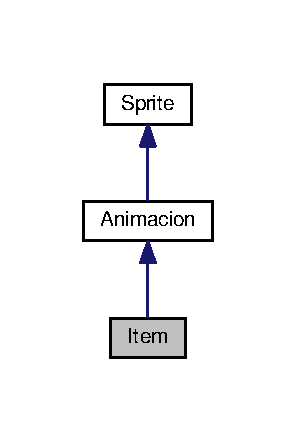
\includegraphics[width=142pt]{class_item__inherit__graph}
\end{center}
\end{figure}


Collaboration diagram for Item\+:\nopagebreak
\begin{figure}[H]
\begin{center}
\leavevmode
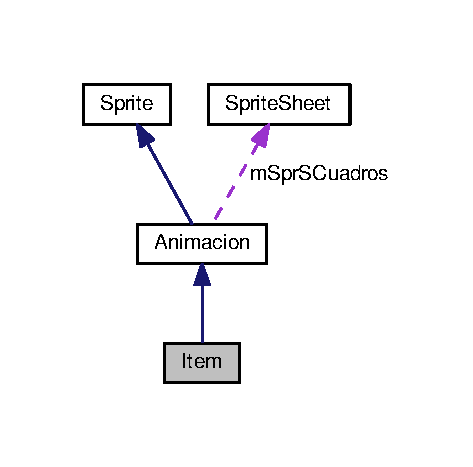
\includegraphics[width=227pt]{class_item__coll__graph}
\end{center}
\end{figure}
\subsection*{Public Types}
\begin{DoxyCompactItemize}
\item 
enum {\bfseries Tipo\+Item} \{ \\*
{\bfseries I\+T\+E\+M\+\_\+\+B\+O\+M\+BA}, 
{\bfseries I\+T\+E\+M\+\_\+\+A\+L\+C\+A\+N\+CE}, 
{\bfseries I\+T\+E\+M\+\_\+\+B\+O\+M\+B\+A\+\_\+\+M\+AX}, 
{\bfseries I\+T\+E\+M\+\_\+\+A\+L\+C\+A\+N\+C\+E\+\_\+\+M\+AX}, 
\\*
{\bfseries I\+T\+E\+M\+\_\+\+A\+T\+R\+A\+V\+I\+E\+S\+A\+\_\+\+B\+O\+M\+B\+AS}, 
{\bfseries I\+T\+E\+M\+\_\+\+M\+U\+E\+R\+TE}, 
{\bfseries I\+T\+E\+M\+\_\+\+P\+R\+O\+T\+E\+C\+C\+I\+ON}, 
{\bfseries I\+T\+E\+M\+\_\+\+C\+O\+N\+T\+R\+O\+L\+A\+\_\+\+B\+O\+M\+BA}, 
\\*
{\bfseries I\+T\+E\+M\+\_\+\+A\+T\+R\+A\+V\+I\+E\+S\+A\+\_\+\+P\+A\+R\+E\+D\+ES}, 
{\bfseries I\+T\+E\+M\+\_\+\+P\+A\+T\+I\+N\+E\+TA}, 
{\bfseries I\+T\+E\+M\+\_\+\+P\+A\+T\+E\+A\+\_\+\+B\+O\+M\+BA}, 
{\bfseries I\+T\+E\+M\+\_\+\+B\+O\+L\+A\+\_\+\+A\+R\+R\+OZ}, 
\\*
{\bfseries I\+T\+E\+M\+\_\+\+G\+U\+A\+N\+TE}, 
{\bfseries I\+T\+E\+M\+\_\+\+P\+U\+E\+R\+TA}, 
{\bfseries I\+T\+E\+M\+\_\+\+V\+I\+DA}, 
{\bfseries I\+T\+E\+M\+\_\+\+R\+E\+L\+OJ}, 
\\*
{\bfseries I\+T\+E\+M\+\_\+\+C\+O\+R\+A\+Z\+ON}, 
{\bfseries I\+T\+E\+M\+\_\+\+P\+A\+S\+T\+EL}, 
{\bfseries I\+T\+E\+M\+\_\+\+A\+L\+E\+A\+T\+O\+R\+IO}, 
{\bfseries I\+T\+E\+M\+\_\+\+M\+A\+R\+T\+I\+L\+LO}, 
\\*
{\bfseries I\+T\+E\+M\+\_\+\+M\+A\+N\+Z\+A\+NA}, 
{\bfseries I\+T\+E\+M\+\_\+\+E\+X\+T\+I\+N\+G\+U\+I\+D\+OR}, 
{\bfseries I\+T\+E\+M\+\_\+\+P\+A\+L\+E\+TA}, 
{\bfseries I\+T\+E\+M\+\_\+\+B\+A\+R\+Q\+U\+I\+L\+LA}, 
\\*
{\bfseries N\+I\+N\+G\+U\+NO}
 \}\hypertarget{class_item_ac27aab342f7f159fc444101ae7a5227a}{}\label{class_item_ac27aab342f7f159fc444101ae7a5227a}

\end{DoxyCompactItemize}
\subsection*{Public Member Functions}
\begin{DoxyCompactItemize}
\item 
{\bfseries Item} (S\+D\+L\+\_\+\+Renderer $\ast$g\+Renderer, string frames, Tipo\+Item tipo, int x=0, int y=0)\hypertarget{class_item_a2c308c75be1a43da9477b33f9af3e3ed}{}\label{class_item_a2c308c75be1a43da9477b33f9af3e3ed}

\item 
Tipo\+Item {\bfseries get\+Tipo} ()\hypertarget{class_item_a6afd68697e76f50a6cd33993c5fcbf12}{}\label{class_item_a6afd68697e76f50a6cd33993c5fcbf12}

\item 
void {\bfseries set\+Player\+Activador} (\hyperlink{class_player}{Player} $\ast$p\+Player)\hypertarget{class_item_a2147bf53d5ba3a1b01c9f916bb91a976}{}\label{class_item_a2147bf53d5ba3a1b01c9f916bb91a976}

\item 
\hyperlink{class_player}{Player} $\ast$ {\bfseries get\+Player\+Activador} ()\hypertarget{class_item_a2c72815d6996dc65e8b76aec6bdd6f97}{}\label{class_item_a2c72815d6996dc65e8b76aec6bdd6f97}

\end{DoxyCompactItemize}
\subsection*{Additional Inherited Members}


The documentation for this class was generated from the following files\+:\begin{DoxyCompactItemize}
\item 
src/objetos/item.\+hpp\item 
src/objetos/item.\+cpp\end{DoxyCompactItemize}

\hypertarget{class_juego}{}\section{Juego Class Reference}
\label{class_juego}\index{Juego@{Juego}}


Inheritance diagram for Juego\+:\nopagebreak
\begin{figure}[H]
\begin{center}
\leavevmode
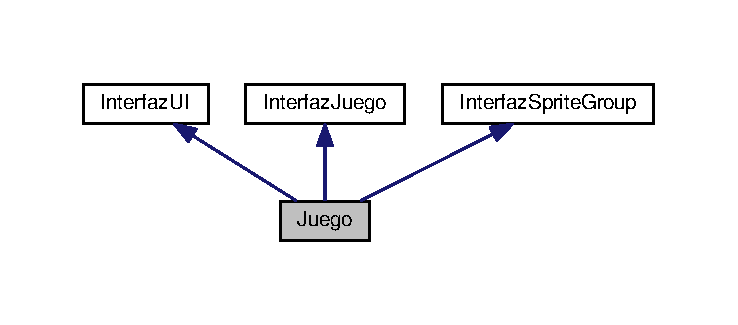
\includegraphics[width=350pt]{class_juego__inherit__graph}
\end{center}
\end{figure}


Collaboration diagram for Juego\+:
\nopagebreak
\begin{figure}[H]
\begin{center}
\leavevmode
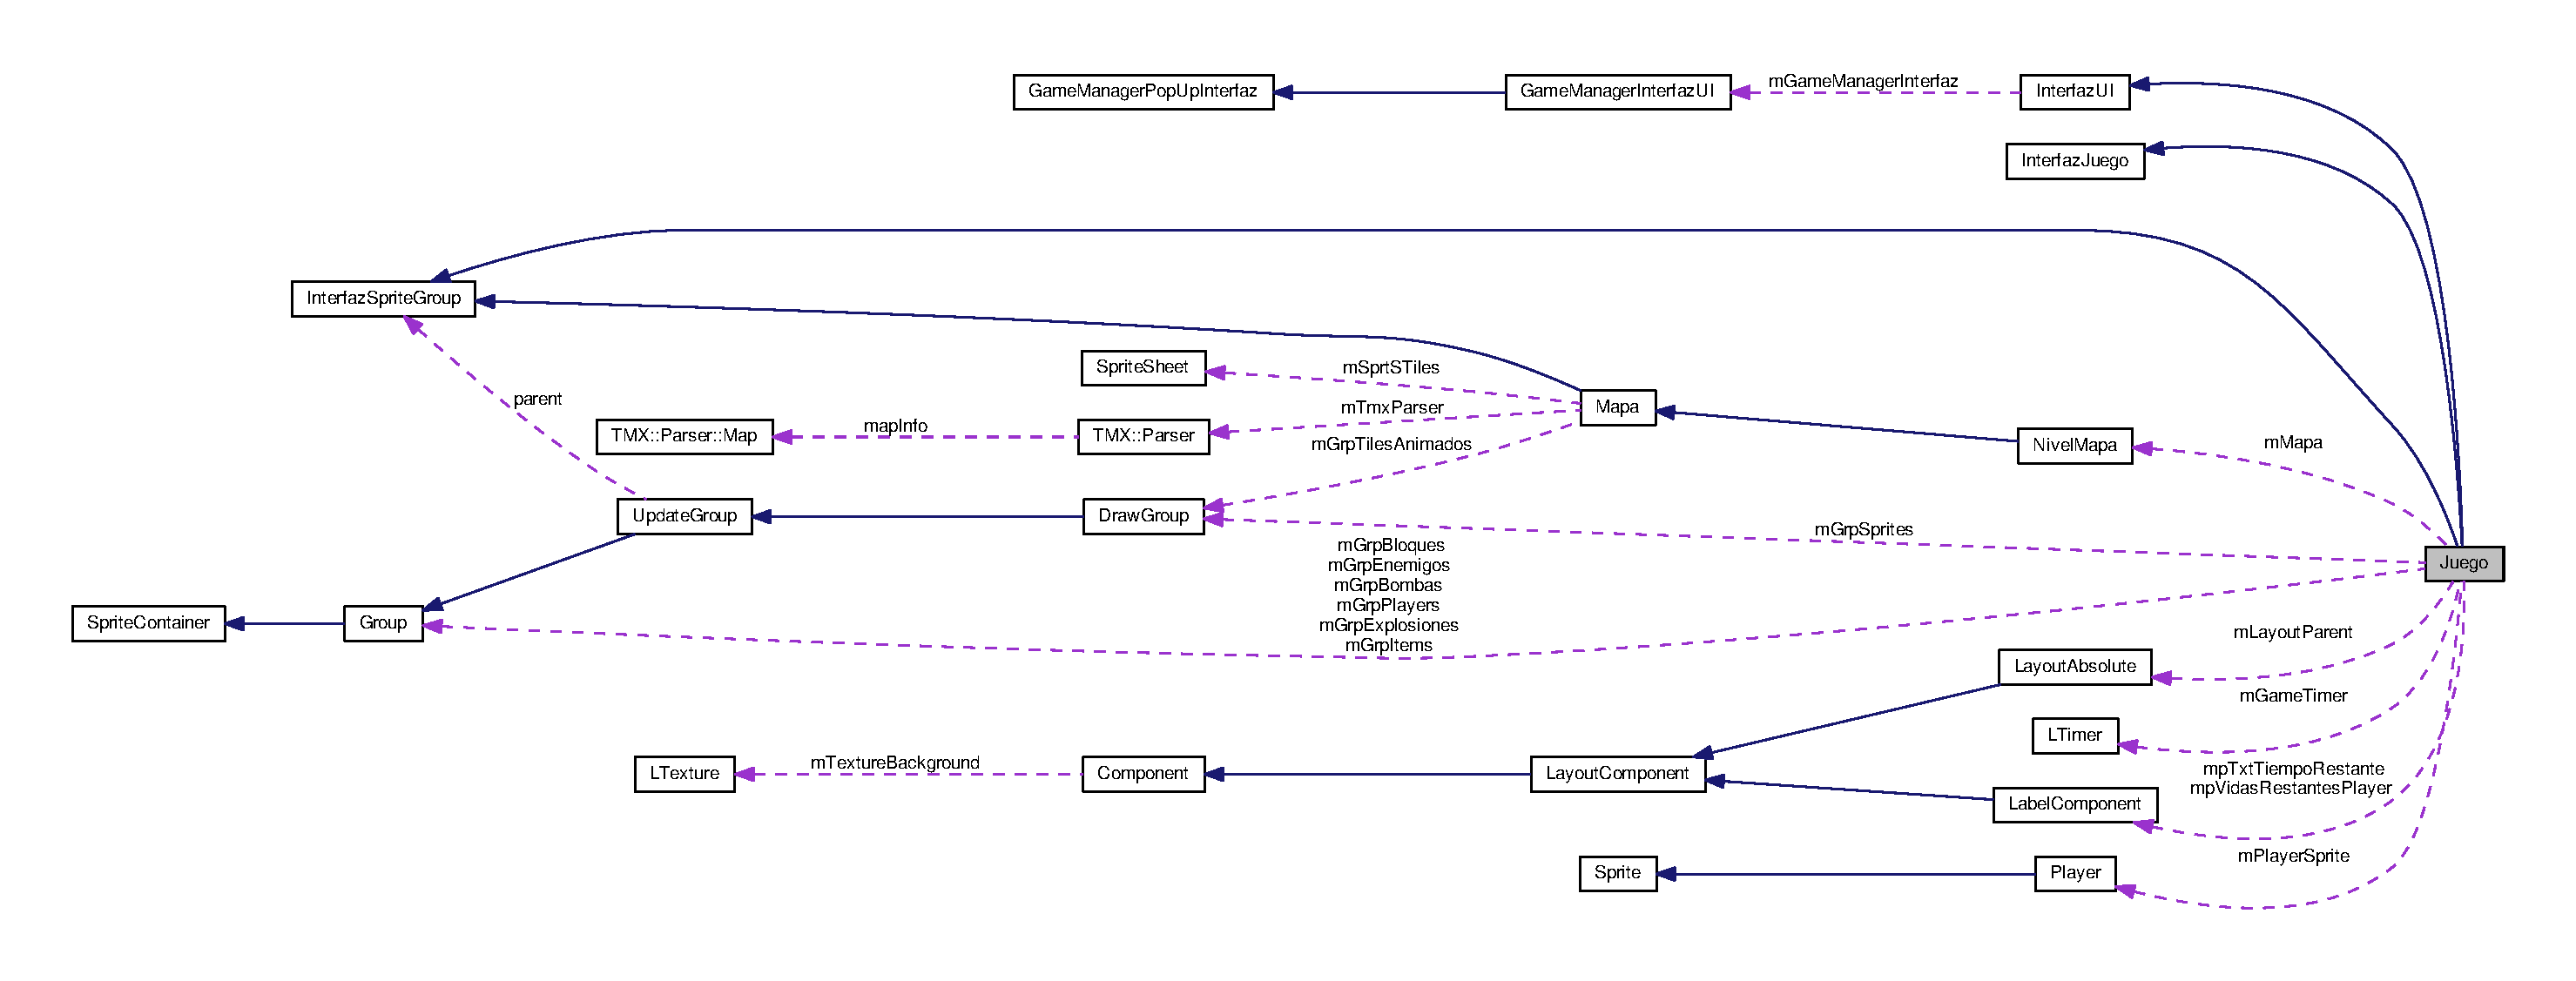
\includegraphics[width=350pt]{class_juego__coll__graph}
\end{center}
\end{figure}
\subsection*{Public Member Functions}
\begin{DoxyCompactItemize}
\item 
\hyperlink{class_juego_aa3d9f9a9d5aa784f583d5f65b304d9e2}{Juego} (\hyperlink{class_game_manager_interfaz_u_i}{Game\+Manager\+Interfaz\+UI} $\ast$game\+Manager, std\+::string ruta\+Mapa, int n\+Victorias, int n\+Minutos, bool is\+Player\+Activo\mbox{[}\+\_\+\+P\+L\+A\+Y\+E\+RS\mbox{]})
\item 
void \hyperlink{class_juego_a5db4a2c61a5853c6a02341d0b9e77cbb}{prepare} () override
\item 
void \hyperlink{class_juego_a8dd19e6a53b446292e3e15e5e164ed05}{create\+UI} (S\+D\+L\+\_\+\+Renderer $\ast$g\+Renderer) override
\item 
void \hyperlink{class_juego_a83e5a1132a5355c34c31d219b4d035dc}{start} () override
\item 
void {\bfseries procesar\+Evento} (S\+D\+L\+\_\+\+Event $\ast$evento) override\hypertarget{class_juego_a67ecc26b162fcdad6471884a0e55f0a0}{}\label{class_juego_a67ecc26b162fcdad6471884a0e55f0a0}

\item 
void \hyperlink{class_juego_a74a8689a0513f13a8dfa6729bae77ada}{update} () override
\item 
void {\bfseries update\+When\+Pop\+Up} () override\hypertarget{class_juego_a6bb98ea5de6c8b4843afd5cd6a811e07}{}\label{class_juego_a6bb98ea5de6c8b4843afd5cd6a811e07}

\item 
void {\bfseries draw} (S\+D\+L\+\_\+\+Renderer $\ast$) override\hypertarget{class_juego_afd62461e81bfd0dcbeecf082f2c023ec}{}\label{class_juego_afd62461e81bfd0dcbeecf082f2c023ec}

\item 
void \hyperlink{class_juego_acaae61b971f3c2b767925db38da41d5c}{eliminar\+Sprite} (\hyperlink{class_sprite}{Sprite} $\ast$sprite) override
\item 
bool {\bfseries is\+Out\+Of\+Map\+Bounds} (S\+D\+L\+\_\+\+Rect rect) override\hypertarget{class_juego_a6d78e56d14ec9985037d213da9c134ff}{}\label{class_juego_a6d78e56d14ec9985037d213da9c134ff}

\item 
\hyperlink{class_bomba}{Bomba} $\ast$ {\bfseries agregar\+Bomba} (\hyperlink{class_player}{Player} $\ast$player\+Propietario) override\hypertarget{class_juego_a7b85a67ebed60f1e80e314f2298951a8}{}\label{class_juego_a7b85a67ebed60f1e80e314f2298951a8}

\item 
deque$<$ \hyperlink{class_sprite}{Sprite} $\ast$ $>$ {\bfseries colision\+Con\+Bombas} (S\+D\+L\+\_\+\+Rect rect) override\hypertarget{class_juego_a4af8340331254c695a0258f22284efe6}{}\label{class_juego_a4af8340331254c695a0258f22284efe6}

\item 
deque$<$ \hyperlink{class_sprite}{Sprite} $\ast$ $>$ {\bfseries colision\+Con\+Explosiones} (S\+D\+L\+\_\+\+Rect rect) override\hypertarget{class_juego_a220161dcde1e991619ac218de9354c5b}{}\label{class_juego_a220161dcde1e991619ac218de9354c5b}

\item 
deque$<$ \hyperlink{class_sprite}{Sprite} $\ast$ $>$ {\bfseries colision\+Bloque\+En\+Llamas} (S\+D\+L\+\_\+\+Rect rect) override\hypertarget{class_juego_a7226f7dd36ef3519b170035afd8ce943}{}\label{class_juego_a7226f7dd36ef3519b170035afd8ce943}

\item 
deque$<$ \hyperlink{class_sprite}{Sprite} $\ast$ $>$ {\bfseries colision\+Con\+Items} (S\+D\+L\+\_\+\+Rect rect) override\hypertarget{class_juego_a0d676fd93f16aff9c9e53fe062b4cbe3}{}\label{class_juego_a0d676fd93f16aff9c9e53fe062b4cbe3}

\item 
Nivel\+Mapa\+::\+Extremo\+Colision {\bfseries colision\+Con\+Mapa} (S\+D\+L\+\_\+\+Rect rect\+\_\+coli, int $\ast$lado\+\_\+colision=nullptr, bool solo\+Bloques\+No\+Traspasables=false) override\hypertarget{class_juego_afc0afb5a5d8dbdc01e15e37c75c77a66}{}\label{class_juego_afc0afb5a5d8dbdc01e15e37c75c77a66}

\item 
int {\bfseries get\+Joys\+Activos} () override\hypertarget{class_juego_a05efa90df1ec93452c715a5da3a88533}{}\label{class_juego_a05efa90df1ec93452c715a5da3a88533}

\item 
S\+D\+L\+\_\+\+Joystick $\ast$ {\bfseries get\+Joy} (int id) override\hypertarget{class_juego_a5bc4a7e470c19d414db169694d0c7775}{}\label{class_juego_a5bc4a7e470c19d414db169694d0c7775}

\item 
\hyperlink{class_l_texture}{L\+Texture} $\ast$ {\bfseries get\+Imagen} (Galeria\+::\+Code\+Imagen code) override\hypertarget{class_juego_a930b36da4b43ff9c9679450fc90b9b8d}{}\label{class_juego_a930b36da4b43ff9c9679450fc90b9b8d}

\item 
\hyperlink{class_tile_en_llamas}{Tile\+En\+Llamas} $\ast$ {\bfseries agregar\+Bloque\+En\+Llamas} (int x, int y) override\hypertarget{class_juego_ab2fc0a295438ebf00813fa36496d0259}{}\label{class_juego_ab2fc0a295438ebf00813fa36496d0259}

\item 
bool {\bfseries es\+Bloque\+Solido} (int x, int y) override\hypertarget{class_juego_a9c9b2f882007b2a43285a3be6d9e0bf2}{}\label{class_juego_a9c9b2f882007b2a43285a3be6d9e0bf2}

\item 
bool {\bfseries es\+Bloque\+Rompible} (int x, int y) override\hypertarget{class_juego_ace6043603d44b94889830d54c1dad8a8}{}\label{class_juego_ace6043603d44b94889830d54c1dad8a8}

\item 
void \hyperlink{class_juego_a336e20deb3bfb1e0717c1bf967ff7a75}{player\+Muerto} (\hyperlink{class_player}{Player} $\ast$p\+Player, \hyperlink{class_sprite}{Sprite} $\ast$p\+Player\+Causante) override
\item 
void {\bfseries pause} () override\hypertarget{class_juego_aaf1cd7159334d07023c78d6b8a35e63f}{}\label{class_juego_aaf1cd7159334d07023c78d6b8a35e63f}

\item 
void {\bfseries resume} () override\hypertarget{class_juego_a3ad516348499c35140e5c61f3e55a6ec}{}\label{class_juego_a3ad516348499c35140e5c61f3e55a6ec}

\item 
void {\bfseries result\+Pop\+Up} (void $\ast$result, int pop\+Up\+Code) override\hypertarget{class_juego_ac141311099a222492201a52842c207b7}{}\label{class_juego_ac141311099a222492201a52842c207b7}

\end{DoxyCompactItemize}
\subsection*{Protected Member Functions}
\begin{DoxyCompactItemize}
\item 
Item\+::\+Tipo\+Item {\bfseries get\+Tipo\+Nuevo\+Item} ()\hypertarget{class_juego_af4734fcef83b06c0a8cfa0ba2a2bc0a7}{}\label{class_juego_af4734fcef83b06c0a8cfa0ba2a2bc0a7}

\item 
void \hyperlink{class_juego_a95af6c1b23ede35e0714e1d01ff7c570}{establecer\+Valores\+De\+Mapa\+Player} (Id\+Player id\+Player)
\item 
void {\bfseries pack\+Layout} (S\+D\+L\+\_\+\+Renderer $\ast$p\+Renderer)\hypertarget{class_juego_a51f2b9d3c31036521eff299b29d98685}{}\label{class_juego_a51f2b9d3c31036521eff299b29d98685}

\item 
void \hyperlink{class_juego_a46d94040c73103aa385d64361717d55c}{draw\+Barra} (S\+D\+L\+\_\+\+Renderer $\ast$)
\item 
void \hyperlink{class_juego_ac40dabed8ef689479cede0b7aa346ce8}{establecer\+Valores\+De\+Mapa\+Players} ()
\item 
void \hyperlink{class_juego_ac4832a99f849b8180667cfda4a2493e3}{agregar\+Players\+Activos} ()
\item 
bool {\bfseries esta\+Player\+Activo} (Id\+Player)\hypertarget{class_juego_a9511541ec77f0dcb380df6f2f49f52e2}{}\label{class_juego_a9511541ec77f0dcb380df6f2f49f52e2}

\item 
void {\bfseries reiniciar\+Estado} ()\hypertarget{class_juego_a0f2054b23552adc7898f67ea4547a980}{}\label{class_juego_a0f2054b23552adc7898f67ea4547a980}

\item 
int {\bfseries get\+Segundos\+Inicio\+Nivel} ()\hypertarget{class_juego_a55223ce1f280cbeff8443196b3334069}{}\label{class_juego_a55223ce1f280cbeff8443196b3334069}

\end{DoxyCompactItemize}
\subsection*{Protected Attributes}
\begin{DoxyCompactItemize}
\item 
\hyperlink{class_draw_group}{Draw\+Group} {\bfseries m\+Grp\+Sprites}\hypertarget{class_juego_a16954a5304977010c10d4a2947904a37}{}\label{class_juego_a16954a5304977010c10d4a2947904a37}

\item 
\hyperlink{class_group}{Group} \hyperlink{class_juego_a21212e537ac309102310b5d6eec8b05d}{m\+Grp\+Enemigos}
\item 
\hyperlink{class_group}{Group} {\bfseries m\+Grp\+Explosiones}\hypertarget{class_juego_afec10123c9056d6dc1094afaf63f9669}{}\label{class_juego_afec10123c9056d6dc1094afaf63f9669}

\item 
\hyperlink{class_group}{Group} {\bfseries m\+Grp\+Items}\hypertarget{class_juego_ad89bd5035fc5f83405888aa142e9507b}{}\label{class_juego_ad89bd5035fc5f83405888aa142e9507b}

\item 
\hyperlink{class_group}{Group} {\bfseries m\+Grp\+Bombas}\hypertarget{class_juego_ad70d8722d5672bfb50a188a81498ad0e}{}\label{class_juego_ad70d8722d5672bfb50a188a81498ad0e}

\item 
\hyperlink{class_group}{Group} {\bfseries m\+Grp\+Players}\hypertarget{class_juego_aefb7102b721b960b92541885939d7340}{}\label{class_juego_aefb7102b721b960b92541885939d7340}

\item 
\hyperlink{class_group}{Group} {\bfseries m\+Grp\+Bloques}\hypertarget{class_juego_a0da19321eebedd555c12fa8097c10945}{}\label{class_juego_a0da19321eebedd555c12fa8097c10945}

\item 
\hyperlink{class_nivel_mapa}{Nivel\+Mapa} {\bfseries m\+Mapa}\hypertarget{class_juego_a1288a8df975edac44f406f5fb3b057f7}{}\label{class_juego_a1288a8df975edac44f406f5fb3b057f7}

\item 
\hyperlink{class_l_timer}{L\+Timer} {\bfseries m\+Game\+Timer}\hypertarget{class_juego_afd3ce8f8b6c1e021c81a09a28a95485d}{}\label{class_juego_afd3ce8f8b6c1e021c81a09a28a95485d}

\item 
int {\bfseries m\+Rondas\+Ganadas} \mbox{[}\+\_\+\+P\+L\+A\+Y\+E\+RS\mbox{]} \{0\}\hypertarget{class_juego_a4ccf29a52fb8b5512521f8e0473b442c}{}\label{class_juego_a4ccf29a52fb8b5512521f8e0473b442c}

\item 
bool {\bfseries m\+Is\+Player\+Activado} \mbox{[}\+\_\+\+P\+L\+A\+Y\+E\+RS\mbox{]} \{false\}\hypertarget{class_juego_a2b5fd9e927e73d550e56ae52b3b5f137}{}\label{class_juego_a2b5fd9e927e73d550e56ae52b3b5f137}

\item 
\hyperlink{class_player}{Player} $\ast$ {\bfseries m\+Player\+Sprite} \mbox{[}\+\_\+\+P\+L\+A\+Y\+E\+RS\mbox{]} \{nullptr\}\hypertarget{class_juego_a6cc0ada2c2041381f84d20843d3e48c7}{}\label{class_juego_a6cc0ada2c2041381f84d20843d3e48c7}

\item 
std\+::string {\bfseries m\+Ruta\+Terreno\+Mapa}\hypertarget{class_juego_ad3a003e0b425815cf01f62277322c6da}{}\label{class_juego_ad3a003e0b425815cf01f62277322c6da}

\item 
int {\bfseries m\+N\+Victorias} = 0\hypertarget{class_juego_ab46d0960968802293c69df8a67309a2f}{}\label{class_juego_ab46d0960968802293c69df8a67309a2f}

\item 
int {\bfseries m\+Minutos} = 0\hypertarget{class_juego_ae8c84e5470394b4908659a53e16679c2}{}\label{class_juego_ae8c84e5470394b4908659a53e16679c2}

\item 
Id\+Player {\bfseries m\+Id\+Lider\+Rondas\+Ganadas} = P\+L\+A\+Y\+E\+R\+\_\+\+N\+O\+NE\hypertarget{class_juego_a8d39c10569fa9c1aa8b0cd66989b3d43}{}\label{class_juego_a8d39c10569fa9c1aa8b0cd66989b3d43}

\item 
S\+D\+L\+\_\+\+Renderer $\ast$ {\bfseries m\+Game\+Renderer}\hypertarget{class_juego_a2dfe5021b437c332a7f5d553502fc9d0}{}\label{class_juego_a2dfe5021b437c332a7f5d553502fc9d0}

\item 
\hyperlink{class_layout_absolute}{Layout\+Absolute} $\ast$ {\bfseries m\+Layout\+Parent}\hypertarget{class_juego_aeac2fc35554cf89683dac4193fc972f9}{}\label{class_juego_aeac2fc35554cf89683dac4193fc972f9}

\item 
\hyperlink{class_label_component}{Label\+Component} $\ast$ {\bfseries mp\+Txt\+Tiempo\+Restante}\hypertarget{class_juego_adda3a8d16fa4706e29da1aee43e92679}{}\label{class_juego_adda3a8d16fa4706e29da1aee43e92679}

\item 
\hyperlink{class_label_component}{Label\+Component} $\ast$ {\bfseries mp\+Vidas\+Restantes\+Player} \mbox{[}\+\_\+\+P\+L\+A\+Y\+E\+RS\mbox{]}\hypertarget{class_juego_a0f8cf53b8d5c8415a8b0c41d9c056c90}{}\label{class_juego_a0f8cf53b8d5c8415a8b0c41d9c056c90}

\item 
bool {\bfseries m\+Is\+Playing\+Warning\+Sound} = false\hypertarget{class_juego_ae07f25bd4865e8892951171f582dc707}{}\label{class_juego_ae07f25bd4865e8892951171f582dc707}

\end{DoxyCompactItemize}
\subsection*{Static Protected Attributes}
\begin{DoxyCompactItemize}
\item 
static const int {\bfseries I\+D\+\_\+\+P\+O\+P\+U\+P\+\_\+\+J\+U\+E\+G\+O\+\_\+\+M\+O\+S\+T\+R\+A\+R\+\_\+\+G\+A\+N\+\_\+\+T\+E\+R\+M\+I\+N\+AR} = 100\hypertarget{class_juego_a5f4d5d2c7acd60f179810e6bfb191cf8}{}\label{class_juego_a5f4d5d2c7acd60f179810e6bfb191cf8}

\item 
static const int {\bfseries I\+D\+\_\+\+P\+O\+P\+U\+P\+\_\+\+J\+U\+E\+G\+O\+\_\+\+M\+O\+S\+T\+R\+A\+R\+\_\+\+G\+A\+N\+\_\+\+C\+O\+N\+T\+I\+N\+U\+AR} = 101\hypertarget{class_juego_a172da2cda4fea948201744d46d281a6c}{}\label{class_juego_a172da2cda4fea948201744d46d281a6c}

\item 
static const int {\bfseries I\+D\+\_\+\+P\+O\+P\+U\+P\+\_\+\+J\+U\+E\+G\+O\+\_\+\+N\+A\+D\+I\+E\+\_\+\+G\+A\+N\+A\+\_\+\+R\+O\+N\+DA} = 102\hypertarget{class_juego_a70048dac849babf67e634558ab45ad83}{}\label{class_juego_a70048dac849babf67e634558ab45ad83}

\item 
static const int {\bfseries I\+D\+\_\+\+P\+O\+P\+U\+P\+\_\+\+J\+U\+E\+G\+O\+\_\+\+C\+O\+M\+I\+E\+N\+ZA} = 103\hypertarget{class_juego_a3c5d91df9c859b59da6087b196d1e8a2}{}\label{class_juego_a3c5d91df9c859b59da6087b196d1e8a2}

\item 
static const int {\bfseries I\+D\+\_\+\+P\+O\+P\+U\+P\+\_\+\+J\+U\+E\+G\+O\+\_\+\+G\+A\+N\+A\+D\+OR} = 104\hypertarget{class_juego_ace2ce255fa30d22737d00caa91962b47}{}\label{class_juego_ace2ce255fa30d22737d00caa91962b47}

\end{DoxyCompactItemize}


\subsection{Constructor \& Destructor Documentation}
\index{Juego@{Juego}!Juego@{Juego}}
\index{Juego@{Juego}!Juego@{Juego}}
\subsubsection[{\texorpdfstring{Juego(\+Game\+Manager\+Interfaz\+U\+I $\ast$game\+Manager, std\+::string ruta\+Mapa, int n\+Victorias, int n\+Minutos, bool is\+Player\+Activo[\+\_\+\+P\+L\+A\+Y\+E\+RS])}{Juego(GameManagerInterfazUI *gameManager, std::string rutaMapa, int nVictorias, int nMinutos, bool isPlayerActivo[_PLAYERS])}}]{\setlength{\rightskip}{0pt plus 5cm}Juego\+::\+Juego (
\begin{DoxyParamCaption}
\item[{{\bf Game\+Manager\+Interfaz\+UI} $\ast$}]{game\+Manager, }
\item[{std\+::string}]{ruta\+Mapa, }
\item[{int}]{n\+Victorias, }
\item[{int}]{n\+Minutos, }
\item[{bool}]{is\+Player\+Activo\mbox{[}\+\_\+\+P\+L\+A\+Y\+E\+R\+S\mbox{]}}
\end{DoxyParamCaption}
)}\hypertarget{class_juego_aa3d9f9a9d5aa784f583d5f65b304d9e2}{}\label{class_juego_aa3d9f9a9d5aa784f583d5f65b304d9e2}
Inicializa la clase \hyperlink{class_juego}{Juego} 
\begin{DoxyParams}{Parameters}
{\em game\+Manager} & \\
\hline
{\em ruta\+Mapa} & Ruta al mapa .tmx \\
\hline
{\em n\+Victorias} & Numero de victorias totales que debe tener un jugador para acabar el juego \\
\hline
{\em n\+Minutos} & Numero de minutos que debe durar como máximo el juego \\
\hline
{\em is\+Player\+Activo} & Array con los players que jugaran \\
\hline
\end{DoxyParams}


\subsection{Member Function Documentation}
\index{Juego@{Juego}!agregar\+Players\+Activos@{agregar\+Players\+Activos}}
\index{agregar\+Players\+Activos@{agregar\+Players\+Activos}!Juego@{Juego}}
\subsubsection[{\texorpdfstring{agregar\+Players\+Activos()}{agregarPlayersActivos()}}]{\setlength{\rightskip}{0pt plus 5cm}void Juego\+::agregar\+Players\+Activos (
\begin{DoxyParamCaption}
{}
\end{DoxyParamCaption}
)\hspace{0.3cm}{\ttfamily [protected]}}\hypertarget{class_juego_ac4832a99f849b8180667cfda4a2493e3}{}\label{class_juego_ac4832a99f849b8180667cfda4a2493e3}
Agrega los players que fueron activados a los grupos del juego Lo cual hace que se actualizen y dibujen \index{Juego@{Juego}!create\+UI@{create\+UI}}
\index{create\+UI@{create\+UI}!Juego@{Juego}}
\subsubsection[{\texorpdfstring{create\+U\+I(\+S\+D\+L\+\_\+\+Renderer $\ast$g\+Renderer) override}{createUI(SDL_Renderer *gRenderer) override}}]{\setlength{\rightskip}{0pt plus 5cm}void Juego\+::create\+UI (
\begin{DoxyParamCaption}
\item[{S\+D\+L\+\_\+\+Renderer $\ast$}]{g\+Renderer}
\end{DoxyParamCaption}
)\hspace{0.3cm}{\ttfamily [override]}, {\ttfamily [virtual]}}\hypertarget{class_juego_a8dd19e6a53b446292e3e15e5e164ed05}{}\label{class_juego_a8dd19e6a53b446292e3e15e5e164ed05}
Crea El layout que se encargara de dibujar los componentes necesarios para la interfaz Tales son los componentes que dibujan el texto en pantalla 
\begin{DoxyParams}{Parameters}
{\em g\+Renderer} & \\
\hline
\end{DoxyParams}


Reimplemented from \hyperlink{class_interfaz_u_i_a9dd59265e0790f06862fdfb12494767e}{Interfaz\+UI}.

\index{Juego@{Juego}!draw\+Barra@{draw\+Barra}}
\index{draw\+Barra@{draw\+Barra}!Juego@{Juego}}
\subsubsection[{\texorpdfstring{draw\+Barra(\+S\+D\+L\+\_\+\+Renderer $\ast$)}{drawBarra(SDL_Renderer *)}}]{\setlength{\rightskip}{0pt plus 5cm}void Juego\+::draw\+Barra (
\begin{DoxyParamCaption}
\item[{S\+D\+L\+\_\+\+Renderer $\ast$}]{g\+Renderer}
\end{DoxyParamCaption}
)\hspace{0.3cm}{\ttfamily [protected]}}\hypertarget{class_juego_a46d94040c73103aa385d64361717d55c}{}\label{class_juego_a46d94040c73103aa385d64361717d55c}
Dibuja los datos que se muestran arriba del \hyperlink{class_mapa}{Mapa} 
\begin{DoxyParams}{Parameters}
{\em g\+Renderer} & \\
\hline
\end{DoxyParams}
\index{Juego@{Juego}!eliminar\+Sprite@{eliminar\+Sprite}}
\index{eliminar\+Sprite@{eliminar\+Sprite}!Juego@{Juego}}
\subsubsection[{\texorpdfstring{eliminar\+Sprite(\+Sprite $\ast$sprite) override}{eliminarSprite(Sprite *sprite) override}}]{\setlength{\rightskip}{0pt plus 5cm}void Juego\+::eliminar\+Sprite (
\begin{DoxyParamCaption}
\item[{{\bf Sprite} $\ast$}]{sprite}
\end{DoxyParamCaption}
)\hspace{0.3cm}{\ttfamily [override]}, {\ttfamily [virtual]}}\hypertarget{class_juego_acaae61b971f3c2b767925db38da41d5c}{}\label{class_juego_acaae61b971f3c2b767925db38da41d5c}
Elimina un \hyperlink{class_sprite}{Sprite} del juego Dependiendo del tipo de sprite a eliminar se hace una accion correspondiente 
\begin{DoxyParams}{Parameters}
{\em sprite} & \\
\hline
\end{DoxyParams}
Si un item es eliminado puede ser \+: Que una explosion lo ha alcanzado y la explosion le aplico kill lo cual lo mando aquí indirectamente Que un player ha colisionado con él y le ha dicho \char`\"{}hey yo te he activado!\char`\"{} y le ha hecho kill() lo cual tambien lo ha mandado aqui. Por lo que al inicio solo obtenemos el player que ha activado el item el cual si ha ocurrido el primer caso debería ser null y por consiguiente se agrega un item en llamas ahí sino entonces se le dice al player \char`\"{}bien hecho toma tu recompensa!\char`\"{}

Implements \hyperlink{class_interfaz_sprite_group_acad50741e8bab94e3ce1f8c4c0cbad52}{Interfaz\+Sprite\+Group}.

\index{Juego@{Juego}!establecer\+Valores\+De\+Mapa\+Player@{establecer\+Valores\+De\+Mapa\+Player}}
\index{establecer\+Valores\+De\+Mapa\+Player@{establecer\+Valores\+De\+Mapa\+Player}!Juego@{Juego}}
\subsubsection[{\texorpdfstring{establecer\+Valores\+De\+Mapa\+Player(\+Id\+Player id\+Player)}{establecerValoresDeMapaPlayer(IdPlayer idPlayer)}}]{\setlength{\rightskip}{0pt plus 5cm}void Juego\+::establecer\+Valores\+De\+Mapa\+Player (
\begin{DoxyParamCaption}
\item[{Id\+Player}]{id\+Player}
\end{DoxyParamCaption}
)\hspace{0.3cm}{\ttfamily [protected]}}\hypertarget{class_juego_a95af6c1b23ede35e0714e1d01ff7c570}{}\label{class_juego_a95af6c1b23ede35e0714e1d01ff7c570}
Establece los valores iniciales de un player establecidos por el \hyperlink{class_mapa}{Mapa} 
\begin{DoxyParams}{Parameters}
{\em id\+Player} & \\
\hline
\end{DoxyParams}
\index{Juego@{Juego}!establecer\+Valores\+De\+Mapa\+Players@{establecer\+Valores\+De\+Mapa\+Players}}
\index{establecer\+Valores\+De\+Mapa\+Players@{establecer\+Valores\+De\+Mapa\+Players}!Juego@{Juego}}
\subsubsection[{\texorpdfstring{establecer\+Valores\+De\+Mapa\+Players()}{establecerValoresDeMapaPlayers()}}]{\setlength{\rightskip}{0pt plus 5cm}void Juego\+::establecer\+Valores\+De\+Mapa\+Players (
\begin{DoxyParamCaption}
{}
\end{DoxyParamCaption}
)\hspace{0.3cm}{\ttfamily [protected]}}\hypertarget{class_juego_ac40dabed8ef689479cede0b7aa346ce8}{}\label{class_juego_ac40dabed8ef689479cede0b7aa346ce8}
Una vez cargado el mapa se deben iniciar los players con los valores iniciales que se establecieron que el mapa especifica \index{Juego@{Juego}!player\+Muerto@{player\+Muerto}}
\index{player\+Muerto@{player\+Muerto}!Juego@{Juego}}
\subsubsection[{\texorpdfstring{player\+Muerto(\+Player $\ast$p\+Player, Sprite $\ast$p\+Player\+Causante) override}{playerMuerto(Player *pPlayer, Sprite *pPlayerCausante) override}}]{\setlength{\rightskip}{0pt plus 5cm}void Juego\+::player\+Muerto (
\begin{DoxyParamCaption}
\item[{{\bf Player} $\ast$}]{p\+Player, }
\item[{{\bf Sprite} $\ast$}]{p\+Player\+Causante}
\end{DoxyParamCaption}
)\hspace{0.3cm}{\ttfamily [override]}, {\ttfamily [virtual]}}\hypertarget{class_juego_a336e20deb3bfb1e0717c1bf967ff7a75}{}\label{class_juego_a336e20deb3bfb1e0717c1bf967ff7a75}
Este metodo es llamado por los players para decir \char`\"{}hey estoy muerto! y este tipo me ha matado! dime que hago\char`\"{} o simplemente \char`\"{}hey estoy muerto dime que hago\char`\"{} 
\begin{DoxyParams}{Parameters}
{\em p\+Player} & \\
\hline
{\em p\+Player\+Causante} & \\
\hline
\end{DoxyParams}


Implements \hyperlink{class_interfaz_juego}{Interfaz\+Juego}.

\index{Juego@{Juego}!prepare@{prepare}}
\index{prepare@{prepare}!Juego@{Juego}}
\subsubsection[{\texorpdfstring{prepare() override}{prepare() override}}]{\setlength{\rightskip}{0pt plus 5cm}void Juego\+::prepare (
\begin{DoxyParamCaption}
{}
\end{DoxyParamCaption}
)\hspace{0.3cm}{\ttfamily [override]}, {\ttfamily [virtual]}}\hypertarget{class_juego_a5db4a2c61a5853c6a02341d0b9e77cbb}{}\label{class_juego_a5db4a2c61a5853c6a02341d0b9e77cbb}
Crea el \hyperlink{class_mapa}{Mapa} los players y el timer 

Reimplemented from \hyperlink{class_interfaz_u_i_a312ba3176f7778589cd67f1828682012}{Interfaz\+UI}.

\index{Juego@{Juego}!start@{start}}
\index{start@{start}!Juego@{Juego}}
\subsubsection[{\texorpdfstring{start() override}{start() override}}]{\setlength{\rightskip}{0pt plus 5cm}void Juego\+::start (
\begin{DoxyParamCaption}
{}
\end{DoxyParamCaption}
)\hspace{0.3cm}{\ttfamily [override]}, {\ttfamily [virtual]}}\hypertarget{class_juego_a83e5a1132a5355c34c31d219b4d035dc}{}\label{class_juego_a83e5a1132a5355c34c31d219b4d035dc}
Inicia el estado del juego 

Reimplemented from \hyperlink{class_interfaz_u_i_a2a80214a4387c21c34a617a8a96996ca}{Interfaz\+UI}.

\index{Juego@{Juego}!update@{update}}
\index{update@{update}!Juego@{Juego}}
\subsubsection[{\texorpdfstring{update() override}{update() override}}]{\setlength{\rightskip}{0pt plus 5cm}void Juego\+::update (
\begin{DoxyParamCaption}
{}
\end{DoxyParamCaption}
)\hspace{0.3cm}{\ttfamily [override]}, {\ttfamily [virtual]}}\hypertarget{class_juego_a74a8689a0513f13a8dfa6729bae77ada}{}\label{class_juego_a74a8689a0513f13a8dfa6729bae77ada}
Actualiza la lógica del juego \}//fin if(!pausado)

controla\+Pausa(teclas);

/$\ast$ switch(estado\+\_\+actual)\{ case P\+L\+AY\+: if(!animando\+Entrada\+Mapa\+Vertical)estado\+Play(); break; case D\+I\+S\+P\+L\+A\+Y\+\_\+\+M\+SG\+: estado\+Display\+Mensage(); break; \} if(animando\+Entrada\+Mapa\+Vertical)\{ desplazamiento+=2; m\+Mapa.\+set\+Eje\+Visualizacion(m\+Mapa.\+get\+Eje\+X(),H\+\_\+\+S\+C\+R\+E\+E\+N-\/desplazamiento); if(H\+\_\+\+S\+C\+R\+E\+E\+N-\/desplazamiento$<$=m\+Mapa.\+get\+Eje\+Y())\{ animando\+Entrada\+Mapa\+Vertical=false; \} \} 

Reimplemented from \hyperlink{class_interfaz_u_i}{Interfaz\+UI}.



\subsection{Member Data Documentation}
\index{Juego@{Juego}!m\+Grp\+Enemigos@{m\+Grp\+Enemigos}}
\index{m\+Grp\+Enemigos@{m\+Grp\+Enemigos}!Juego@{Juego}}
\subsubsection[{\texorpdfstring{m\+Grp\+Enemigos}{mGrpEnemigos}}]{\setlength{\rightskip}{0pt plus 5cm}{\bf Group} Juego\+::m\+Grp\+Enemigos\hspace{0.3cm}{\ttfamily [protected]}}\hypertarget{class_juego_a21212e537ac309102310b5d6eec8b05d}{}\label{class_juego_a21212e537ac309102310b5d6eec8b05d}
Grupo para cada ente que es colisionable, para manejarlo por separado Si bien se puede manejar con solo m\+Grp\+Sprites, cuando se detecta una colision entonces habria que estar viendo si lo que se regreso es un sprite del tipo que se quiere. 

The documentation for this class was generated from the following files\+:\begin{DoxyCompactItemize}
\item 
src/\+Interfaces/juego/juego.\+hpp\item 
src/\+Interfaces/juego/juego.\+cpp\end{DoxyCompactItemize}

\hypertarget{class_label_component}{}\section{Label\+Component Class Reference}
\label{class_label_component}\index{Label\+Component@{Label\+Component}}


Inheritance diagram for Label\+Component\+:
\nopagebreak
\begin{figure}[H]
\begin{center}
\leavevmode
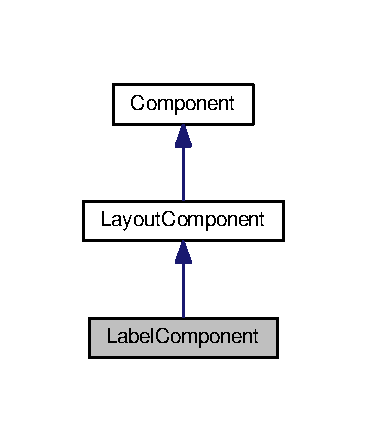
\includegraphics[width=176pt]{class_label_component__inherit__graph}
\end{center}
\end{figure}


Collaboration diagram for Label\+Component\+:
\nopagebreak
\begin{figure}[H]
\begin{center}
\leavevmode
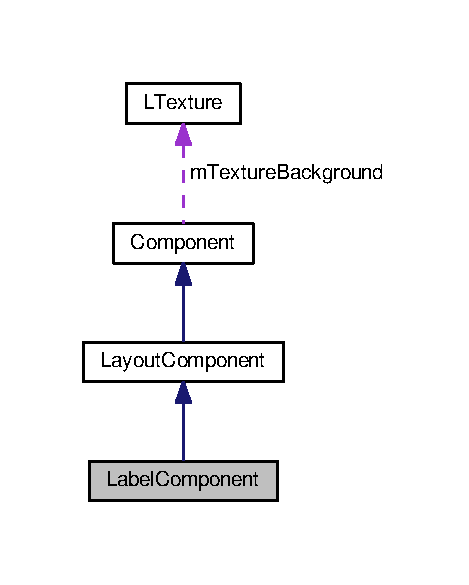
\includegraphics[width=225pt]{class_label_component__coll__graph}
\end{center}
\end{figure}
\subsection*{Public Member Functions}
\begin{DoxyCompactItemize}
\item 
void {\bfseries set\+Text} (string nuevo\+Texto)\hypertarget{class_label_component_a0ed2e841847a3fcd745097a6daee50ba}{}\label{class_label_component_a0ed2e841847a3fcd745097a6daee50ba}

\item 
void {\bfseries set\+Font} (\hyperlink{class_c_font}{C\+Font} $\ast$nueva\+Fuente)\hypertarget{class_label_component_a1fc48a3b8c8807d73688c57442c8d2c1}{}\label{class_label_component_a1fc48a3b8c8807d73688c57442c8d2c1}

\item 
void \hyperlink{class_label_component_a9979a17ac60f351d9850e0d670d8ab0e}{pack} (S\+D\+L\+\_\+\+Renderer $\ast$g\+Renderer)
\item 
void \hyperlink{class_label_component_a9637b7af88eb351108ef490f175b39a9}{draw} (S\+D\+L\+\_\+\+Renderer $\ast$g\+Renderer) override
\item 
void {\bfseries set\+Text\+Color} (S\+D\+L\+\_\+\+Color nuevo)\hypertarget{class_label_component_aecb3f36a01c1c4f5bc924d8f4041bfc9}{}\label{class_label_component_aecb3f36a01c1c4f5bc924d8f4041bfc9}

\item 
void {\bfseries set\+Text\+Size} (int nueva\+Size)\hypertarget{class_label_component_a74dca5480528e2748a20368e909ebdf8}{}\label{class_label_component_a74dca5480528e2748a20368e909ebdf8}

\item 
void {\bfseries set\+Font} (string ruta\+Fuente, int size)\hypertarget{class_label_component_a436f611099bc24618624fca6b4a6de3a}{}\label{class_label_component_a436f611099bc24618624fca6b4a6de3a}

\end{DoxyCompactItemize}
\subsection*{Additional Inherited Members}


\subsection{Detailed Description}
\begin{Desc}
\item[Examples\+: ]\par
\hyperlink{_2home_2manuggz_2_documents_2_projects_2_bomberman_2src_2engine_2interfaces_2_menu_list_label_8hpp-example}{/home/manuggz/\+Documents/\+Projects/\+Bomberman/src/engine/interfaces/\+Menu\+List\+Label.\+hpp}.\end{Desc}


\subsection{Member Function Documentation}
\index{Label\+Component@{Label\+Component}!draw@{draw}}
\index{draw@{draw}!Label\+Component@{Label\+Component}}
\subsubsection[{\texorpdfstring{draw(\+S\+D\+L\+\_\+\+Renderer $\ast$g\+Renderer) override}{draw(SDL_Renderer *gRenderer) override}}]{\setlength{\rightskip}{0pt plus 5cm}void Label\+Component\+::draw (
\begin{DoxyParamCaption}
\item[{S\+D\+L\+\_\+\+Renderer $\ast$}]{g\+Renderer}
\end{DoxyParamCaption}
)\hspace{0.3cm}{\ttfamily [inline]}, {\ttfamily [override]}, {\ttfamily [virtual]}}\hypertarget{class_label_component_a9637b7af88eb351108ef490f175b39a9}{}\label{class_label_component_a9637b7af88eb351108ef490f175b39a9}
Dibuja el componente 
\begin{DoxyParams}{Parameters}
{\em g\+Renderer} & \\
\hline
\end{DoxyParams}


Reimplemented from \hyperlink{class_component_ab1ea202c9ef8933d15956b96cfe281a1}{Component}.

\index{Label\+Component@{Label\+Component}!pack@{pack}}
\index{pack@{pack}!Label\+Component@{Label\+Component}}
\subsubsection[{\texorpdfstring{pack(\+S\+D\+L\+\_\+\+Renderer $\ast$g\+Renderer)}{pack(SDL_Renderer *gRenderer)}}]{\setlength{\rightskip}{0pt plus 5cm}void Label\+Component\+::pack (
\begin{DoxyParamCaption}
\item[{S\+D\+L\+\_\+\+Renderer $\ast$}]{g\+Renderer}
\end{DoxyParamCaption}
)\hspace{0.3cm}{\ttfamily [inline]}, {\ttfamily [virtual]}}\hypertarget{class_label_component_a9979a17ac60f351d9850e0d670d8ab0e}{}\label{class_label_component_a9979a17ac60f351d9850e0d670d8ab0e}
Se encarga de crear las texturas del componente asi como otras acciones asociadas con el renderer Notar que despues de esta funcion se debe llamar a calculate\+Rect, es decir, realizar una nueva calculacion del rectangulo de dibujo del componente 
\begin{DoxyParams}{Parameters}
{\em g\+Renderer} & Render de la pantalla \\
\hline
\end{DoxyParams}


Implements \hyperlink{class_component_aa471f2c3a24525f584ed19cf25222e70}{Component}.



The documentation for this class was generated from the following file\+:\begin{DoxyCompactItemize}
\item 
src/engine/layout/\+Componentes/Label\+Component.\+hpp\end{DoxyCompactItemize}

\hypertarget{class_layout_absolute}{}\section{Layout\+Absolute Class Reference}
\label{class_layout_absolute}\index{Layout\+Absolute@{Layout\+Absolute}}


Inheritance diagram for Layout\+Absolute\+:\nopagebreak
\begin{figure}[H]
\begin{center}
\leavevmode
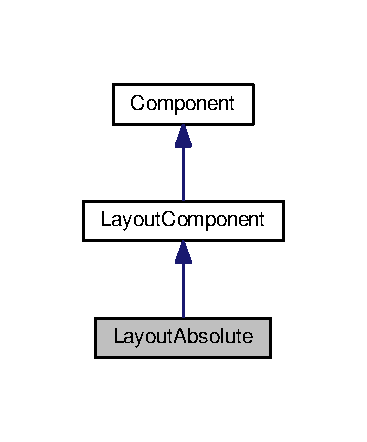
\includegraphics[width=176pt]{class_layout_absolute__inherit__graph}
\end{center}
\end{figure}


Collaboration diagram for Layout\+Absolute\+:\nopagebreak
\begin{figure}[H]
\begin{center}
\leavevmode
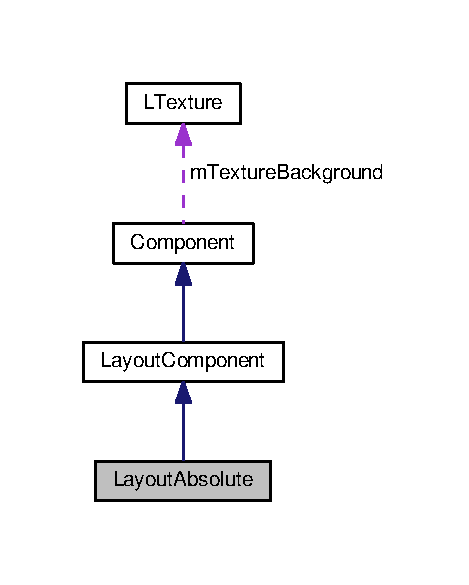
\includegraphics[width=225pt]{class_layout_absolute__coll__graph}
\end{center}
\end{figure}
\subsection*{Public Member Functions}
\begin{DoxyCompactItemize}
\item 
void {\bfseries add\+Component} (\hyperlink{class_component}{Component} $\ast$nuevo\+Componente)\hypertarget{class_layout_absolute_adc08dc77ab5168e496f3edc3a41c4326}{}\label{class_layout_absolute_adc08dc77ab5168e496f3edc3a41c4326}

\item 
bool \hyperlink{class_layout_absolute_aba1ab3840e566a65bdecb4ba8a249eac}{is\+Disabled} ()
\item 
void \hyperlink{class_layout_absolute_a9807517212f0015c0a67399a35f1ff36}{pack} (S\+D\+L\+\_\+\+Renderer $\ast$g\+Renderer) override
\item 
void \hyperlink{class_layout_absolute_a09327626b1406cdfad158c13353f0c86}{set\+Rect\+Dibujo} (S\+D\+L\+\_\+\+Rect \&rect) override
\end{DoxyCompactItemize}
\subsection*{Additional Inherited Members}


\subsection{Member Function Documentation}
\index{Layout\+Absolute@{Layout\+Absolute}!is\+Disabled@{is\+Disabled}}
\index{is\+Disabled@{is\+Disabled}!Layout\+Absolute@{Layout\+Absolute}}
\subsubsection[{\texorpdfstring{is\+Disabled()}{isDisabled()}}]{\setlength{\rightskip}{0pt plus 5cm}bool Layout\+Absolute\+::is\+Disabled (
\begin{DoxyParamCaption}
{}
\end{DoxyParamCaption}
)\hspace{0.3cm}{\ttfamily [inline]}, {\ttfamily [virtual]}}\hypertarget{class_layout_absolute_aba1ab3840e566a65bdecb4ba8a249eac}{}\label{class_layout_absolute_aba1ab3840e566a65bdecb4ba8a249eac}
Chequea si hay algun componente con disable = true o si el layout en si esta en ese estado \begin{DoxyReturn}{Returns}
True si hay alguno con ese estado 
\end{DoxyReturn}


Reimplemented from \hyperlink{class_component_aedd9acaa31b5c50a8cf233014b85c0cc}{Component}.

\index{Layout\+Absolute@{Layout\+Absolute}!pack@{pack}}
\index{pack@{pack}!Layout\+Absolute@{Layout\+Absolute}}
\subsubsection[{\texorpdfstring{pack(\+S\+D\+L\+\_\+\+Renderer $\ast$g\+Renderer) override}{pack(SDL_Renderer *gRenderer) override}}]{\setlength{\rightskip}{0pt plus 5cm}void Layout\+Absolute\+::pack (
\begin{DoxyParamCaption}
\item[{S\+D\+L\+\_\+\+Renderer $\ast$}]{g\+Renderer}
\end{DoxyParamCaption}
)\hspace{0.3cm}{\ttfamily [inline]}, {\ttfamily [override]}, {\ttfamily [virtual]}}\hypertarget{class_layout_absolute_a9807517212f0015c0a67399a35f1ff36}{}\label{class_layout_absolute_a9807517212f0015c0a67399a35f1ff36}
Llama a los compactadores de los componentes agregados 
\begin{DoxyParams}{Parameters}
{\em g\+Renderer} & \\
\hline
\end{DoxyParams}


Implements \hyperlink{class_component_aa471f2c3a24525f584ed19cf25222e70}{Component}.

\index{Layout\+Absolute@{Layout\+Absolute}!set\+Rect\+Dibujo@{set\+Rect\+Dibujo}}
\index{set\+Rect\+Dibujo@{set\+Rect\+Dibujo}!Layout\+Absolute@{Layout\+Absolute}}
\subsubsection[{\texorpdfstring{set\+Rect\+Dibujo(\+S\+D\+L\+\_\+\+Rect \&rect) override}{setRectDibujo(SDL_Rect &rect) override}}]{\setlength{\rightskip}{0pt plus 5cm}void Layout\+Absolute\+::set\+Rect\+Dibujo (
\begin{DoxyParamCaption}
\item[{S\+D\+L\+\_\+\+Rect \&}]{rect}
\end{DoxyParamCaption}
)\hspace{0.3cm}{\ttfamily [inline]}, {\ttfamily [override]}, {\ttfamily [virtual]}}\hypertarget{class_layout_absolute_a09327626b1406cdfad158c13353f0c86}{}\label{class_layout_absolute_a09327626b1406cdfad158c13353f0c86}
Dibuja el layout y sus componentes de arriba hacia abajo / verticalmente 
\begin{DoxyParams}{Parameters}
{\em renderer} & \\
\hline
\end{DoxyParams}


Reimplemented from \hyperlink{class_component}{Component}.



The documentation for this class was generated from the following file\+:\begin{DoxyCompactItemize}
\item 
src/engine/layout/\+Layout\+Manager/Layout\+Absolute.\+hpp\end{DoxyCompactItemize}

\hypertarget{class_layout_component}{}\section{Layout\+Component Class Reference}
\label{class_layout_component}\index{Layout\+Component@{Layout\+Component}}


Inheritance diagram for Layout\+Component\+:
\nopagebreak
\begin{figure}[H]
\begin{center}
\leavevmode
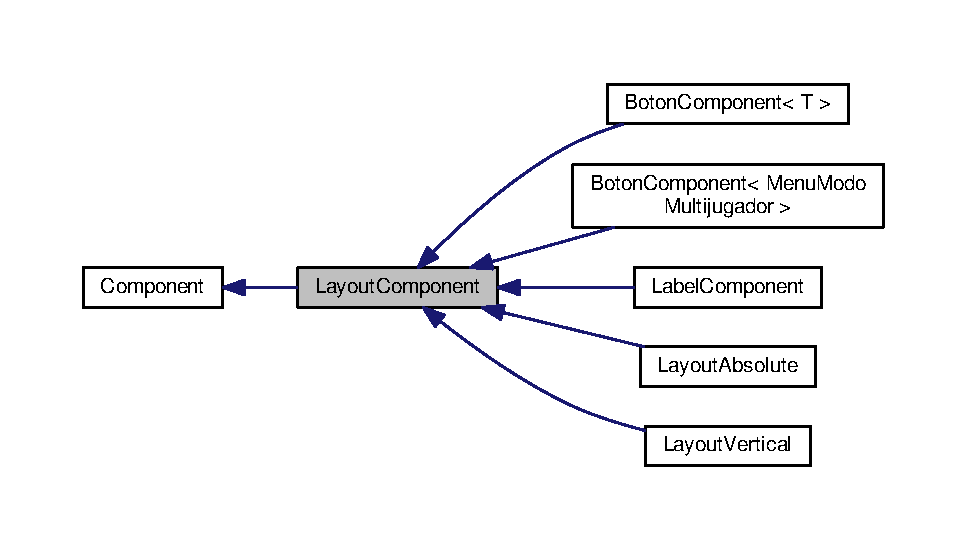
\includegraphics[width=350pt]{class_layout_component__inherit__graph}
\end{center}
\end{figure}


Collaboration diagram for Layout\+Component\+:\nopagebreak
\begin{figure}[H]
\begin{center}
\leavevmode
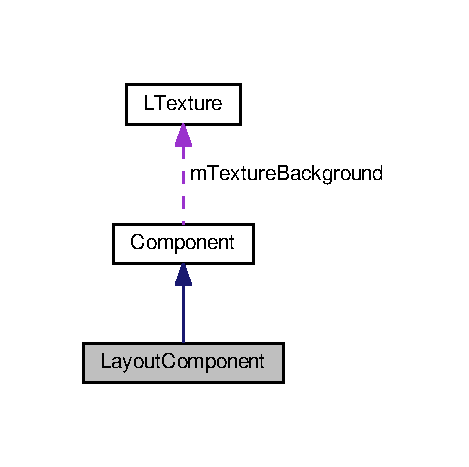
\includegraphics[width=225pt]{class_layout_component__coll__graph}
\end{center}
\end{figure}
\subsection*{Public Member Functions}
\begin{DoxyCompactItemize}
\item 
void \hyperlink{class_layout_component_a0ee8a3146a3258a9886472b86cf34a16}{draw} (S\+D\+L\+\_\+\+Renderer $\ast$g\+Renderer) override
\end{DoxyCompactItemize}
\subsection*{Protected Attributes}
\begin{DoxyCompactItemize}
\item 
std\+::deque$<$ \hyperlink{class_component}{Component} $\ast$ $>$ {\bfseries m\+Componentes}\hypertarget{class_layout_component_aee117bd6f1a520cfbdeddca847cc2833}{}\label{class_layout_component_aee117bd6f1a520cfbdeddca847cc2833}

\end{DoxyCompactItemize}


\subsection{Member Function Documentation}
\index{Layout\+Component@{Layout\+Component}!draw@{draw}}
\index{draw@{draw}!Layout\+Component@{Layout\+Component}}
\subsubsection[{\texorpdfstring{draw(\+S\+D\+L\+\_\+\+Renderer $\ast$g\+Renderer) override}{draw(SDL_Renderer *gRenderer) override}}]{\setlength{\rightskip}{0pt plus 5cm}void Layout\+Component\+::draw (
\begin{DoxyParamCaption}
\item[{S\+D\+L\+\_\+\+Renderer $\ast$}]{g\+Renderer}
\end{DoxyParamCaption}
)\hspace{0.3cm}{\ttfamily [inline]}, {\ttfamily [override]}, {\ttfamily [virtual]}}\hypertarget{class_layout_component_a0ee8a3146a3258a9886472b86cf34a16}{}\label{class_layout_component_a0ee8a3146a3258a9886472b86cf34a16}
Dibuja el layout y sus componentes de arriba hacia abajo / verticalmente 
\begin{DoxyParams}{Parameters}
{\em renderer} & \\
\hline
\end{DoxyParams}


Reimplemented from \hyperlink{class_component_ab1ea202c9ef8933d15956b96cfe281a1}{Component}.



Reimplemented in \hyperlink{class_boton_component_a73c8c3014be82c952cd8d0e08beffcc5}{Boton\+Component$<$ Menu\+Modo\+Multijugador $>$}.

\begin{Desc}
\item[Examples\+: ]\par
\hyperlink{_2home_2manuggz_2_documents_2_projects_2_bomberman_2src_2engine_2interfaces_2_menu_list_label_8hpp-example}{/home/manuggz/\+Documents/\+Projects/\+Bomberman/src/engine/interfaces/\+Menu\+List\+Label.\+hpp}.\end{Desc}


The documentation for this class was generated from the following file\+:\begin{DoxyCompactItemize}
\item 
src/engine/layout/\+Layout\+Manager/Layout\+Component.\+hpp\end{DoxyCompactItemize}

\hypertarget{class_layout_parent}{}\section{Layout\+Parent Class Reference}
\label{class_layout_parent}\index{Layout\+Parent@{Layout\+Parent}}
\subsection*{Public Member Functions}
\begin{DoxyCompactItemize}
\item 
{\bfseries Layout\+Parent} (\hyperlink{class_layout_component}{Layout\+Component} $\ast$layout)\hypertarget{class_layout_parent_abbde1c8867bcdcecd296fce84cc10627}{}\label{class_layout_parent_abbde1c8867bcdcecd296fce84cc10627}

\item 
void \hyperlink{class_layout_parent_a07f39188ee96ac0a3f545d3e24d948c4}{establecer\+Rect\+Dibujo} (S\+D\+L\+\_\+\+Rect \&g\+Renderer)
\end{DoxyCompactItemize}


\subsection{Member Function Documentation}
\index{Layout\+Parent@{Layout\+Parent}!establecer\+Rect\+Dibujo@{establecer\+Rect\+Dibujo}}
\index{establecer\+Rect\+Dibujo@{establecer\+Rect\+Dibujo}!Layout\+Parent@{Layout\+Parent}}
\subsubsection[{\texorpdfstring{establecer\+Rect\+Dibujo(\+S\+D\+L\+\_\+\+Rect \&g\+Renderer)}{establecerRectDibujo(SDL_Rect &gRenderer)}}]{\setlength{\rightskip}{0pt plus 5cm}void Layout\+Parent\+::establecer\+Rect\+Dibujo (
\begin{DoxyParamCaption}
\item[{S\+D\+L\+\_\+\+Rect \&}]{g\+Renderer}
\end{DoxyParamCaption}
)\hspace{0.3cm}{\ttfamily [inline]}}\hypertarget{class_layout_parent_a07f39188ee96ac0a3f545d3e24d948c4}{}\label{class_layout_parent_a07f39188ee96ac0a3f545d3e24d948c4}
Dibuja el m\+Layout y sus componentes de arriba hacia abajo / verticalmente 
\begin{DoxyParams}{Parameters}
{\em renderer} & \\
\hline
\end{DoxyParams}


The documentation for this class was generated from the following file\+:\begin{DoxyCompactItemize}
\item 
src/engine/layout/\+Layout\+Manager/Layout\+Parent.\+hpp\end{DoxyCompactItemize}

\hypertarget{class_layout_vertical}{}\section{Layout\+Vertical Class Reference}
\label{class_layout_vertical}\index{Layout\+Vertical@{Layout\+Vertical}}


Inheritance diagram for Layout\+Vertical\+:\nopagebreak
\begin{figure}[H]
\begin{center}
\leavevmode
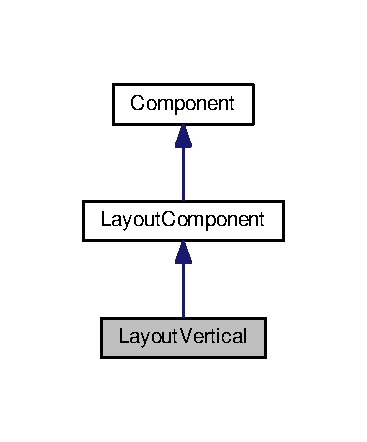
\includegraphics[width=176pt]{class_layout_vertical__inherit__graph}
\end{center}
\end{figure}


Collaboration diagram for Layout\+Vertical\+:\nopagebreak
\begin{figure}[H]
\begin{center}
\leavevmode
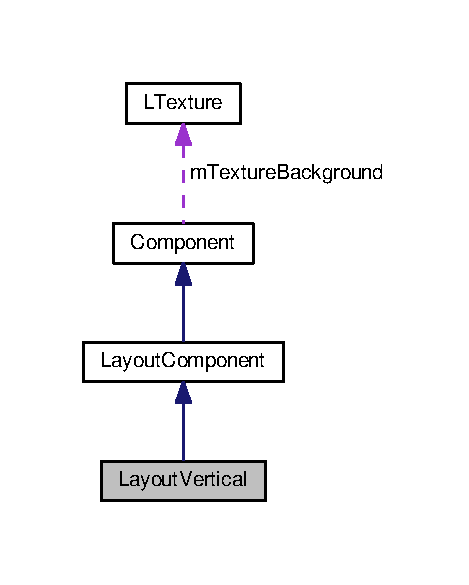
\includegraphics[width=225pt]{class_layout_vertical__coll__graph}
\end{center}
\end{figure}
\subsection*{Public Member Functions}
\begin{DoxyCompactItemize}
\item 
void {\bfseries add\+Component} (\hyperlink{class_component}{Component} $\ast$nuevo\+Componente)\hypertarget{class_layout_vertical_a3d675e4ba5f0e1c45b78a8191eaf3b15}{}\label{class_layout_vertical_a3d675e4ba5f0e1c45b78a8191eaf3b15}

\item 
bool \hyperlink{class_layout_vertical_a90f1b16b40a8765bb59d536b667e13e4}{is\+Disabled} ()
\item 
void \hyperlink{class_layout_vertical_a02eea5b9dd8197100d964d0e6f33e208}{pack} (S\+D\+L\+\_\+\+Renderer $\ast$g\+Renderer) override
\item 
virtual void {\bfseries set\+Rect\+Dibujo} (S\+D\+L\+\_\+\+Rect \&rect) override\hypertarget{class_layout_vertical_a08fbc2283e2cb2c42c806fe21f64a0ac}{}\label{class_layout_vertical_a08fbc2283e2cb2c42c806fe21f64a0ac}

\end{DoxyCompactItemize}
\subsection*{Additional Inherited Members}


\subsection{Detailed Description}
\begin{Desc}
\item[Examples\+: ]\par
\hyperlink{_2home_2manuggz_2_documents_2_projects_2_bomberman_2src_2engine_2interfaces_2_menu_list_label_8hpp-example}{/home/manuggz/\+Documents/\+Projects/\+Bomberman/src/engine/interfaces/\+Menu\+List\+Label.\+hpp}.\end{Desc}


\subsection{Member Function Documentation}
\index{Layout\+Vertical@{Layout\+Vertical}!is\+Disabled@{is\+Disabled}}
\index{is\+Disabled@{is\+Disabled}!Layout\+Vertical@{Layout\+Vertical}}
\subsubsection[{\texorpdfstring{is\+Disabled()}{isDisabled()}}]{\setlength{\rightskip}{0pt plus 5cm}bool Layout\+Vertical\+::is\+Disabled (
\begin{DoxyParamCaption}
{}
\end{DoxyParamCaption}
)\hspace{0.3cm}{\ttfamily [inline]}, {\ttfamily [virtual]}}\hypertarget{class_layout_vertical_a90f1b16b40a8765bb59d536b667e13e4}{}\label{class_layout_vertical_a90f1b16b40a8765bb59d536b667e13e4}
Chequea si hay algun componente con disable = true o si el layout en si esta en ese estado \begin{DoxyReturn}{Returns}
True si hay alguno con ese estado 
\end{DoxyReturn}


Reimplemented from \hyperlink{class_component_aedd9acaa31b5c50a8cf233014b85c0cc}{Component}.

\begin{Desc}
\item[Examples\+: ]\par
\hyperlink{_2home_2manuggz_2_documents_2_projects_2_bomberman_2src_2engine_2interfaces_2_menu_list_label_8hpp-example}{/home/manuggz/\+Documents/\+Projects/\+Bomberman/src/engine/interfaces/\+Menu\+List\+Label.\+hpp}.\end{Desc}
\index{Layout\+Vertical@{Layout\+Vertical}!pack@{pack}}
\index{pack@{pack}!Layout\+Vertical@{Layout\+Vertical}}
\subsubsection[{\texorpdfstring{pack(\+S\+D\+L\+\_\+\+Renderer $\ast$g\+Renderer) override}{pack(SDL_Renderer *gRenderer) override}}]{\setlength{\rightskip}{0pt plus 5cm}void Layout\+Vertical\+::pack (
\begin{DoxyParamCaption}
\item[{S\+D\+L\+\_\+\+Renderer $\ast$}]{g\+Renderer}
\end{DoxyParamCaption}
)\hspace{0.3cm}{\ttfamily [inline]}, {\ttfamily [override]}, {\ttfamily [virtual]}}\hypertarget{class_layout_vertical_a02eea5b9dd8197100d964d0e6f33e208}{}\label{class_layout_vertical_a02eea5b9dd8197100d964d0e6f33e208}
Llama a los compactadores de los componentes agregados 
\begin{DoxyParams}{Parameters}
{\em g\+Renderer} & \\
\hline
\end{DoxyParams}


Implements \hyperlink{class_component_aa471f2c3a24525f584ed19cf25222e70}{Component}.

\begin{Desc}
\item[Examples\+: ]\par
\hyperlink{_2home_2manuggz_2_documents_2_projects_2_bomberman_2src_2engine_2interfaces_2_menu_list_label_8hpp-example}{/home/manuggz/\+Documents/\+Projects/\+Bomberman/src/engine/interfaces/\+Menu\+List\+Label.\+hpp}.\end{Desc}


The documentation for this class was generated from the following file\+:\begin{DoxyCompactItemize}
\item 
src/engine/layout/\+Layout\+Manager/Layout\+Vertical.\+hpp\end{DoxyCompactItemize}

\hypertarget{class_l_texture}{}\section{L\+Texture Class Reference}
\label{class_l_texture}\index{L\+Texture@{L\+Texture}}
\subsection*{Public Member Functions}
\begin{DoxyCompactItemize}
\item 
bool {\bfseries load\+From\+File} (std\+::string path, S\+D\+L\+\_\+\+Renderer $\ast$g\+Rendered, bool tiene\+Color\+Clave)\hypertarget{class_l_texture_a25b90cb830a0d7a5705a72da006a9571}{}\label{class_l_texture_a25b90cb830a0d7a5705a72da006a9571}

\item 
bool {\bfseries load\+From\+Rendered\+Text} (S\+D\+L\+\_\+\+Renderer $\ast$g\+Renderer, T\+T\+F\+\_\+\+Font $\ast$g\+Font, std\+::string texture\+Text, S\+D\+L\+\_\+\+Color text\+Color)\hypertarget{class_l_texture_a1ef989f4fc5f7f8c0897203437219a8b}{}\label{class_l_texture_a1ef989f4fc5f7f8c0897203437219a8b}

\item 
void {\bfseries free} ()\hypertarget{class_l_texture_abef558f0b920270079925548a3976a06}{}\label{class_l_texture_abef558f0b920270079925548a3976a06}

\item 
Uint32 {\bfseries getpixel} (int x, int y)\hypertarget{class_l_texture_ad26a88237a60b3bbc1822bb4e1f47048}{}\label{class_l_texture_ad26a88237a60b3bbc1822bb4e1f47048}

\item 
void {\bfseries set\+Color} (Uint8 red, Uint8 green, Uint8 blue)\hypertarget{class_l_texture_a4ccf201515ecb158b137394d41ed9077}{}\label{class_l_texture_a4ccf201515ecb158b137394d41ed9077}

\item 
void {\bfseries set\+Blend\+Mode} (S\+D\+L\+\_\+\+Blend\+Mode blending)\hypertarget{class_l_texture_aa1fe07070f715bf3981c129ae1619a4e}{}\label{class_l_texture_aa1fe07070f715bf3981c129ae1619a4e}

\item 
void {\bfseries set\+Alpha} (Uint8 alpha)\hypertarget{class_l_texture_ab4e51b54752ae7b54614078f9128a9c0}{}\label{class_l_texture_ab4e51b54752ae7b54614078f9128a9c0}

\item 
void {\bfseries render} (S\+D\+L\+\_\+\+Renderer $\ast$g\+Renderer, int x=0, int y=0, S\+D\+L\+\_\+\+Rect $\ast$clip=N\+U\+LL, double angle=0.\+0, S\+D\+L\+\_\+\+Point $\ast$center=N\+U\+LL, S\+D\+L\+\_\+\+Renderer\+Flip flip=S\+D\+L\+\_\+\+F\+L\+I\+P\+\_\+\+N\+O\+NE)\hypertarget{class_l_texture_a7edbf22bd4e3f5efd60e20b913d1dcc4}{}\label{class_l_texture_a7edbf22bd4e3f5efd60e20b913d1dcc4}

\item 
int {\bfseries get\+Width} () const \hypertarget{class_l_texture_ad9e83e3ba49b7ef6a0719ddbbdf7b3fa}{}\label{class_l_texture_ad9e83e3ba49b7ef6a0719ddbbdf7b3fa}

\item 
int {\bfseries get\+Height} () const \hypertarget{class_l_texture_a88f3901941f4a71f929845ee1311b68b}{}\label{class_l_texture_a88f3901941f4a71f929845ee1311b68b}

\item 
std\+::string {\bfseries get\+Path} () const \hypertarget{class_l_texture_a70aa0ad5a0d095498b5e29a0575c8ff5}{}\label{class_l_texture_a70aa0ad5a0d095498b5e29a0575c8ff5}

\end{DoxyCompactItemize}


The documentation for this class was generated from the following files\+:\begin{DoxyCompactItemize}
\item 
src/engine/util/L\+Texture.\+hpp\item 
src/engine/util/L\+Texture.\+cpp\end{DoxyCompactItemize}

\hypertarget{class_l_timer}{}\section{L\+Timer Class Reference}
\label{class_l_timer}\index{L\+Timer@{L\+Timer}}
\subsection*{Public Member Functions}
\begin{DoxyCompactItemize}
\item 
void {\bfseries start} ()\hypertarget{class_l_timer_a7dc11f05cf5098a6d06ebd6ebec96ed6}{}\label{class_l_timer_a7dc11f05cf5098a6d06ebd6ebec96ed6}

\item 
void {\bfseries stop} ()\hypertarget{class_l_timer_aeabbf5f935907fcfeaa7f4403741e4ae}{}\label{class_l_timer_aeabbf5f935907fcfeaa7f4403741e4ae}

\item 
void {\bfseries pause} ()\hypertarget{class_l_timer_a8a6c6af5435bdaa825a30f84877dc059}{}\label{class_l_timer_a8a6c6af5435bdaa825a30f84877dc059}

\item 
void {\bfseries resume} ()\hypertarget{class_l_timer_a27355a22a0a159e8e48e9fe1529399f0}{}\label{class_l_timer_a27355a22a0a159e8e48e9fe1529399f0}

\item 
Uint32 {\bfseries get\+Ticks} ()\hypertarget{class_l_timer_a57c4bdca0f7bdd75c65b6ab1499de1e7}{}\label{class_l_timer_a57c4bdca0f7bdd75c65b6ab1499de1e7}

\item 
bool {\bfseries is\+Started} ()\hypertarget{class_l_timer_a102ca688eaa4109dd733b4b60a29d27c}{}\label{class_l_timer_a102ca688eaa4109dd733b4b60a29d27c}

\item 
bool {\bfseries is\+Paused} ()\hypertarget{class_l_timer_ae1d9b504da6ed0f42e10f2338a9f88bb}{}\label{class_l_timer_ae1d9b504da6ed0f42e10f2338a9f88bb}

\item 
bool {\bfseries is\+Running} ()\hypertarget{class_l_timer_a103d426dfcf480bc3938ef41023af629}{}\label{class_l_timer_a103d426dfcf480bc3938ef41023af629}

\end{DoxyCompactItemize}


The documentation for this class was generated from the following files\+:\begin{DoxyCompactItemize}
\item 
src/engine/util/L\+Timer.\+hpp\item 
src/engine/util/L\+Timer.\+cpp\end{DoxyCompactItemize}

\hypertarget{struct_t_m_x_1_1_parser_1_1_map}{}\section{T\+MX\+:\+:Parser\+:\+:Map Struct Reference}
\label{struct_t_m_x_1_1_parser_1_1_map}\index{T\+M\+X\+::\+Parser\+::\+Map@{T\+M\+X\+::\+Parser\+::\+Map}}
\subsection*{Public Attributes}
\begin{DoxyCompactItemize}
\item 
std\+::string {\bfseries version}\hypertarget{struct_t_m_x_1_1_parser_1_1_map_ab457e6705cc3f3a39147a539307b635f}{}\label{struct_t_m_x_1_1_parser_1_1_map_ab457e6705cc3f3a39147a539307b635f}

\item 
std\+::string {\bfseries orientation}\hypertarget{struct_t_m_x_1_1_parser_1_1_map_a945dfd673bafc7f96aa1474e18963cb6}{}\label{struct_t_m_x_1_1_parser_1_1_map_a945dfd673bafc7f96aa1474e18963cb6}

\item 
unsigned int {\bfseries width}\hypertarget{struct_t_m_x_1_1_parser_1_1_map_a4338d3f05dc42b14f603aa8ce1413d67}{}\label{struct_t_m_x_1_1_parser_1_1_map_a4338d3f05dc42b14f603aa8ce1413d67}

\item 
unsigned int {\bfseries height}\hypertarget{struct_t_m_x_1_1_parser_1_1_map_abf57bc2c65496718c6bdea647e0d0ec1}{}\label{struct_t_m_x_1_1_parser_1_1_map_abf57bc2c65496718c6bdea647e0d0ec1}

\item 
unsigned int {\bfseries tile\+Width}\hypertarget{struct_t_m_x_1_1_parser_1_1_map_adf712cbd57543e77156de25cbfc6145b}{}\label{struct_t_m_x_1_1_parser_1_1_map_adf712cbd57543e77156de25cbfc6145b}

\item 
unsigned int {\bfseries tile\+Height}\hypertarget{struct_t_m_x_1_1_parser_1_1_map_a8171070658368818d4d4a4f1ba48a065}{}\label{struct_t_m_x_1_1_parser_1_1_map_a8171070658368818d4d4a4f1ba48a065}

\item 
std\+::string {\bfseries background\+Color}\hypertarget{struct_t_m_x_1_1_parser_1_1_map_ac719e47959e1b66d9689bfbc0b91dccd}{}\label{struct_t_m_x_1_1_parser_1_1_map_ac719e47959e1b66d9689bfbc0b91dccd}

\item 
std\+::map$<$ std\+::string, std\+::string $>$ {\bfseries property}\hypertarget{struct_t_m_x_1_1_parser_1_1_map_aca5abf5c028b13b3105ee2622b67a29f}{}\label{struct_t_m_x_1_1_parser_1_1_map_aca5abf5c028b13b3105ee2622b67a29f}

\end{DoxyCompactItemize}


The documentation for this struct was generated from the following file\+:\begin{DoxyCompactItemize}
\item 
src/engine/mapa/include/T\+M\+X\+Parser.\+h\end{DoxyCompactItemize}

\hypertarget{class_mapa}{}\section{Mapa Class Reference}
\label{class_mapa}\index{Mapa@{Mapa}}


Inheritance diagram for Mapa\+:
\nopagebreak
\begin{figure}[H]
\begin{center}
\leavevmode
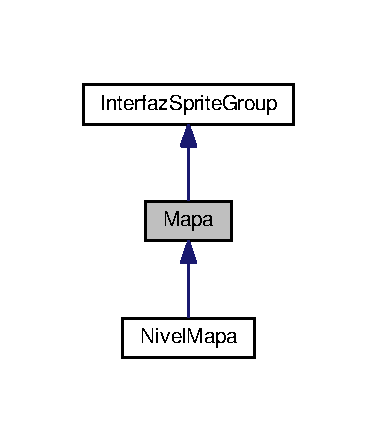
\includegraphics[width=181pt]{class_mapa__inherit__graph}
\end{center}
\end{figure}


Collaboration diagram for Mapa\+:
\nopagebreak
\begin{figure}[H]
\begin{center}
\leavevmode
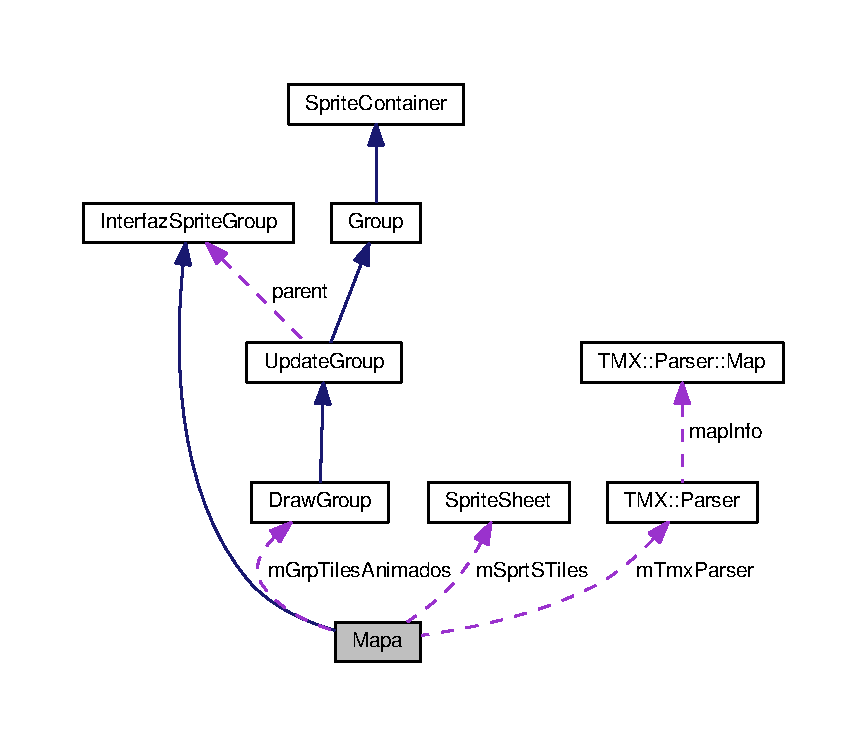
\includegraphics[width=350pt]{class_mapa__coll__graph}
\end{center}
\end{figure}
\subsection*{Public Member Functions}
\begin{DoxyCompactItemize}
\item 
{\bfseries Mapa} (int x, int y)\hypertarget{class_mapa_a2a88268f7c620deb8d2561e18a57f0c3}{}\label{class_mapa_a2a88268f7c620deb8d2561e18a57f0c3}

\item 
void \hyperlink{class_mapa_a142d3bbb3a2166aa575b90e50c790a36}{eliminar\+Sprite} (\hyperlink{class_sprite}{Sprite} $\ast$sprite) override
\item 
virtual bool \hyperlink{class_mapa_a25d45fc6b9c1622f8261a0c849a78294}{cargar} (S\+D\+L\+\_\+\+Renderer $\ast$g\+Renderer, std\+::string ruta)
\item 
void {\bfseries update} ()\hypertarget{class_mapa_a5e592dd55f2fd9cf82aa453237260bce}{}\label{class_mapa_a5e592dd55f2fd9cf82aa453237260bce}

\item 
virtual void {\bfseries draw} (S\+D\+L\+\_\+\+Renderer $\ast$g\+Renderer)\hypertarget{class_mapa_a978c5caf727e7f7ee739cd7eb9a690ce}{}\label{class_mapa_a978c5caf727e7f7ee739cd7eb9a690ce}

\item 
const std\+::string \& {\bfseries get\+Map\+Property} (std\+::basic\+\_\+string$<$ char, std\+::char\+\_\+traits$<$ char $>$, std\+::allocator$<$ char $>$$>$ property\+Name)\hypertarget{class_mapa_a169f2cb4198d7933d88099fb16042b9f}{}\label{class_mapa_a169f2cb4198d7933d88099fb16042b9f}

\end{DoxyCompactItemize}
\subsection*{Protected Attributes}
\begin{DoxyCompactItemize}
\item 
\hyperlink{class_t_m_x_1_1_parser}{T\+M\+X\+::\+Parser} $\ast$ {\bfseries m\+Tmx\+Parser} = nullptr\hypertarget{class_mapa_aa1930968e5c377c8c256f63c1e4d6301}{}\label{class_mapa_aa1930968e5c377c8c256f63c1e4d6301}

\item 
\hyperlink{class_sprite_sheet}{Sprite\+Sheet} $\ast$ {\bfseries m\+Sprt\+S\+Tiles} = nullptr\hypertarget{class_mapa_a8967581c875d0a6c070251d9b66345db}{}\label{class_mapa_a8967581c875d0a6c070251d9b66345db}

\item 
int $\ast$ {\bfseries m\+Layer\+Mapa}\hypertarget{class_mapa_a8ee1595b26f941cff5d8ff0474d202f2}{}\label{class_mapa_a8ee1595b26f941cff5d8ff0474d202f2}

\item 
S\+D\+L\+\_\+\+Rect {\bfseries m\+Rect\+Dest} \{0,0,0,0\}\hypertarget{class_mapa_a8d98267cf15cc550f25db96d441c6201}{}\label{class_mapa_a8d98267cf15cc550f25db96d441c6201}

\item 
unsigned int {\bfseries m\+Tile\+Height} = 0\hypertarget{class_mapa_a38c77f72272f53e38cf355c988e5eaa6}{}\label{class_mapa_a38c77f72272f53e38cf355c988e5eaa6}

\item 
unsigned int {\bfseries m\+Map\+Width} = 0\hypertarget{class_mapa_ac2c8daa280f568a6d78c4641eedec9d9}{}\label{class_mapa_ac2c8daa280f568a6d78c4641eedec9d9}

\item 
unsigned int {\bfseries m\+Map\+Height} = 0\hypertarget{class_mapa_a1a7fd0909905efb7f890e98baffde43c}{}\label{class_mapa_a1a7fd0909905efb7f890e98baffde43c}

\item 
unsigned int {\bfseries m\+Tile\+Width} = 0\hypertarget{class_mapa_a4db442f40a4972f78726b04dbb259e02}{}\label{class_mapa_a4db442f40a4972f78726b04dbb259e02}

\item 
\hyperlink{class_draw_group}{Draw\+Group} {\bfseries m\+Grp\+Tiles\+Animados}\hypertarget{class_mapa_af73f2d6413457cd0c82be76ce5050d85}{}\label{class_mapa_af73f2d6413457cd0c82be76ce5050d85}

\end{DoxyCompactItemize}


\subsection{Member Function Documentation}
\index{Mapa@{Mapa}!cargar@{cargar}}
\index{cargar@{cargar}!Mapa@{Mapa}}
\subsubsection[{\texorpdfstring{cargar(\+S\+D\+L\+\_\+\+Renderer $\ast$g\+Renderer, std\+::string ruta)}{cargar(SDL_Renderer *gRenderer, std::string ruta)}}]{\setlength{\rightskip}{0pt plus 5cm}virtual bool Mapa\+::cargar (
\begin{DoxyParamCaption}
\item[{S\+D\+L\+\_\+\+Renderer $\ast$}]{g\+Renderer, }
\item[{std\+::string}]{ruta}
\end{DoxyParamCaption}
)\hspace{0.3cm}{\ttfamily [inline]}, {\ttfamily [virtual]}}\hypertarget{class_mapa_a25d45fc6b9c1622f8261a0c849a78294}{}\label{class_mapa_a25d45fc6b9c1622f8261a0c849a78294}
Carga los datos de un mapa de un archivo T\+MX El archivo T\+MX esta creado en Tiled 
\begin{DoxyParams}{Parameters}
{\em g\+Renderer} & \\
\hline
{\em ruta} & \\
\hline
\end{DoxyParams}
\begin{DoxyReturn}{Returns}

\end{DoxyReturn}
Creamos el mapa con los indices\index{Mapa@{Mapa}!eliminar\+Sprite@{eliminar\+Sprite}}
\index{eliminar\+Sprite@{eliminar\+Sprite}!Mapa@{Mapa}}
\subsubsection[{\texorpdfstring{eliminar\+Sprite(\+Sprite $\ast$sprite) override}{eliminarSprite(Sprite *sprite) override}}]{\setlength{\rightskip}{0pt plus 5cm}void Mapa\+::eliminar\+Sprite (
\begin{DoxyParamCaption}
\item[{{\bf Sprite} $\ast$}]{}
\end{DoxyParamCaption}
)\hspace{0.3cm}{\ttfamily [inline]}, {\ttfamily [override]}, {\ttfamily [virtual]}}\hypertarget{class_mapa_a142d3bbb3a2166aa575b90e50c790a36}{}\label{class_mapa_a142d3bbb3a2166aa575b90e50c790a36}
Elimina un \hyperlink{class_sprite}{Sprite} de Memoria. Esta función es llamada desde un Update\+Group/\+Derivado cuando se elimina un \hyperlink{class_sprite}{Sprite} con kill(). 

Implements \hyperlink{class_interfaz_sprite_group_acad50741e8bab94e3ce1f8c4c0cbad52}{Interfaz\+Sprite\+Group}.



The documentation for this class was generated from the following file\+:\begin{DoxyCompactItemize}
\item 
src/engine/mapa/C\+Mapa.\+hpp\end{DoxyCompactItemize}

\hypertarget{classrapidxml_1_1memory__pool}{}\section{rapidxml\+:\+:memory\+\_\+pool$<$ Ch $>$ Class Template Reference}
\label{classrapidxml_1_1memory__pool}\index{rapidxml\+::memory\+\_\+pool$<$ Ch $>$@{rapidxml\+::memory\+\_\+pool$<$ Ch $>$}}


{\ttfamily \#include $<$rapidxml.\+hpp$>$}



Inheritance diagram for rapidxml\+:\+:memory\+\_\+pool$<$ Ch $>$\+:\nopagebreak
\begin{figure}[H]
\begin{center}
\leavevmode
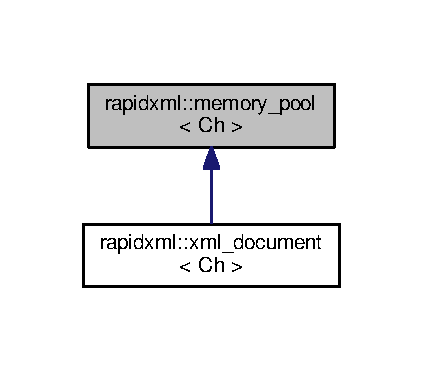
\includegraphics[width=203pt]{classrapidxml_1_1memory__pool__inherit__graph}
\end{center}
\end{figure}
\subsection*{Public Member Functions}
\begin{DoxyCompactItemize}
\item 
\hyperlink{classrapidxml_1_1memory__pool_a0b609da81dff28a19ebd704400788429}{memory\+\_\+pool} ()\hypertarget{classrapidxml_1_1memory__pool_a0b609da81dff28a19ebd704400788429}{}\label{classrapidxml_1_1memory__pool_a0b609da81dff28a19ebd704400788429}

\begin{DoxyCompactList}\small\item\em Constructs empty pool with default allocator functions. \end{DoxyCompactList}\item 
\hyperlink{classrapidxml_1_1memory__pool_a0a3e82126e59e4077f41e933130bb5a0}{$\sim$memory\+\_\+pool} ()
\item 
\hyperlink{classrapidxml_1_1xml__node}{xml\+\_\+node}$<$ Ch $>$ $\ast$ \hyperlink{classrapidxml_1_1memory__pool_a4118581c29ee9a2f6b55ebf7dac185f8}{allocate\+\_\+node} (\hyperlink{rapidxml_8hpp_abb456db38f7efb746c4330eed6072a7c}{node\+\_\+type} type, const Ch $\ast$name=0, const Ch $\ast$value=0, std\+::size\+\_\+t name\+\_\+size=0, std\+::size\+\_\+t value\+\_\+size=0)
\item 
\hyperlink{classrapidxml_1_1xml__attribute}{xml\+\_\+attribute}$<$ Ch $>$ $\ast$ \hyperlink{classrapidxml_1_1memory__pool_a3de2a66c983336e006ea3844e244ed30}{allocate\+\_\+attribute} (const Ch $\ast$name=0, const Ch $\ast$value=0, std\+::size\+\_\+t name\+\_\+size=0, std\+::size\+\_\+t value\+\_\+size=0)
\item 
Ch $\ast$ \hyperlink{classrapidxml_1_1memory__pool_a171941b39d55b868358da97462185f58}{allocate\+\_\+string} (const Ch $\ast$source=0, std\+::size\+\_\+t size=0)
\item 
\hyperlink{classrapidxml_1_1xml__node}{xml\+\_\+node}$<$ Ch $>$ $\ast$ \hyperlink{classrapidxml_1_1memory__pool_a0a10679fc17597d339a0dc107f8a94ac}{clone\+\_\+node} (const \hyperlink{classrapidxml_1_1xml__node}{xml\+\_\+node}$<$ Ch $>$ $\ast$source, \hyperlink{classrapidxml_1_1xml__node}{xml\+\_\+node}$<$ Ch $>$ $\ast$result=0)
\item 
void \hyperlink{classrapidxml_1_1memory__pool_aad377c835fdaed1cb2cc9df194cf84e4}{clear} ()
\item 
void \hyperlink{classrapidxml_1_1memory__pool_a84d3d8d2cdfc00501e1dcf26d889ae03}{set\+\_\+allocator} (alloc\+\_\+func $\ast$af, free\+\_\+func $\ast$ff)
\end{DoxyCompactItemize}


\subsection{Detailed Description}
\subsubsection*{template$<$class Ch = char$>$\\*
class rapidxml\+::memory\+\_\+pool$<$ Ch $>$}

This class is used by the parser to create new nodes and attributes, without overheads of dynamic memory allocation. In most cases, you will not need to use this class directly. However, if you need to create nodes manually or modify names/values of nodes, you are encouraged to use \hyperlink{classrapidxml_1_1memory__pool}{memory\+\_\+pool} of relevant \hyperlink{classrapidxml_1_1xml__document}{xml\+\_\+document} to allocate the memory. Not only is this faster than allocating them by using {\ttfamily new} operator, but also their lifetime will be tied to the lifetime of document, possibly simplyfing memory management. ~\newline
~\newline
 Call \hyperlink{classrapidxml_1_1memory__pool_a4118581c29ee9a2f6b55ebf7dac185f8}{allocate\+\_\+node()} or \hyperlink{classrapidxml_1_1memory__pool_a3de2a66c983336e006ea3844e244ed30}{allocate\+\_\+attribute()} functions to obtain new nodes or attributes from the pool. You can also call \hyperlink{classrapidxml_1_1memory__pool_a171941b39d55b868358da97462185f58}{allocate\+\_\+string()} function to allocate strings. Such strings can then be used as names or values of nodes without worrying about their lifetime. Note that there is no {\ttfamily free()} function -- all allocations are freed at once when \hyperlink{classrapidxml_1_1memory__pool_aad377c835fdaed1cb2cc9df194cf84e4}{clear()} function is called, or when the pool is destroyed. ~\newline
~\newline
 It is also possible to create a standalone \hyperlink{classrapidxml_1_1memory__pool}{memory\+\_\+pool}, and use it to allocate nodes, whose lifetime will not be tied to any document. ~\newline
~\newline
 Pool maintains {\ttfamily R\+A\+P\+I\+D\+X\+M\+L\+\_\+\+S\+T\+A\+T\+I\+C\+\_\+\+P\+O\+O\+L\+\_\+\+S\+I\+ZE} bytes of statically allocated memory. Until static memory is exhausted, no dynamic memory allocations are done. When static memory is exhausted, pool allocates additional blocks of memory of size {\ttfamily R\+A\+P\+I\+D\+X\+M\+L\+\_\+\+D\+Y\+N\+A\+M\+I\+C\+\_\+\+P\+O\+O\+L\+\_\+\+S\+I\+ZE} each, by using global {\ttfamily new\mbox{[}\mbox{]}} and {\ttfamily delete\mbox{[}\mbox{]}} operators. This behaviour can be changed by setting custom allocation routines. Use \hyperlink{classrapidxml_1_1memory__pool_a84d3d8d2cdfc00501e1dcf26d889ae03}{set\+\_\+allocator()} function to set them. ~\newline
~\newline
 Allocations for nodes, attributes and strings are aligned at {\ttfamily R\+A\+P\+I\+D\+X\+M\+L\+\_\+\+A\+L\+I\+G\+N\+M\+E\+NT} bytes. This value defaults to the size of pointer on target architecture. ~\newline
~\newline
 To obtain absolutely top performance from the parser, it is important that all nodes are allocated from a single, contiguous block of memory. Otherwise, cache misses when jumping between two (or more) disjoint blocks of memory can slow down parsing quite considerably. If required, you can tweak {\ttfamily R\+A\+P\+I\+D\+X\+M\+L\+\_\+\+S\+T\+A\+T\+I\+C\+\_\+\+P\+O\+O\+L\+\_\+\+S\+I\+ZE}, {\ttfamily R\+A\+P\+I\+D\+X\+M\+L\+\_\+\+D\+Y\+N\+A\+M\+I\+C\+\_\+\+P\+O\+O\+L\+\_\+\+S\+I\+ZE} and {\ttfamily R\+A\+P\+I\+D\+X\+M\+L\+\_\+\+A\+L\+I\+G\+N\+M\+E\+NT} to obtain best wasted memory to performance compromise. To do it, define their values before \hyperlink{rapidxml_8hpp}{rapidxml.\+hpp} file is included. 
\begin{DoxyParams}{Parameters}
{\em Ch} & Character type of created nodes. \\
\hline
\end{DoxyParams}


\subsection{Constructor \& Destructor Documentation}
\index{rapidxml\+::memory\+\_\+pool@{rapidxml\+::memory\+\_\+pool}!````~memory\+\_\+pool@{$\sim$memory\+\_\+pool}}
\index{````~memory\+\_\+pool@{$\sim$memory\+\_\+pool}!rapidxml\+::memory\+\_\+pool@{rapidxml\+::memory\+\_\+pool}}
\subsubsection[{\texorpdfstring{$\sim$memory\+\_\+pool()}{~memory_pool()}}]{\setlength{\rightskip}{0pt plus 5cm}template$<$class Ch  = char$>$ {\bf rapidxml\+::memory\+\_\+pool}$<$ Ch $>$\+::$\sim${\bf memory\+\_\+pool} (
\begin{DoxyParamCaption}
{}
\end{DoxyParamCaption}
)\hspace{0.3cm}{\ttfamily [inline]}}\hypertarget{classrapidxml_1_1memory__pool_a0a3e82126e59e4077f41e933130bb5a0}{}\label{classrapidxml_1_1memory__pool_a0a3e82126e59e4077f41e933130bb5a0}
Destroys pool and frees all the memory. This causes memory occupied by nodes allocated by the pool to be freed. Nodes allocated from the pool are no longer valid. 

\subsection{Member Function Documentation}
\index{rapidxml\+::memory\+\_\+pool@{rapidxml\+::memory\+\_\+pool}!allocate\+\_\+attribute@{allocate\+\_\+attribute}}
\index{allocate\+\_\+attribute@{allocate\+\_\+attribute}!rapidxml\+::memory\+\_\+pool@{rapidxml\+::memory\+\_\+pool}}
\subsubsection[{\texorpdfstring{allocate\+\_\+attribute(const Ch $\ast$name=0, const Ch $\ast$value=0, std\+::size\+\_\+t name\+\_\+size=0, std\+::size\+\_\+t value\+\_\+size=0)}{allocate_attribute(const Ch *name=0, const Ch *value=0, std::size_t name_size=0, std::size_t value_size=0)}}]{\setlength{\rightskip}{0pt plus 5cm}template$<$class Ch  = char$>$ {\bf xml\+\_\+attribute}$<$Ch$>$$\ast$ {\bf rapidxml\+::memory\+\_\+pool}$<$ Ch $>$\+::allocate\+\_\+attribute (
\begin{DoxyParamCaption}
\item[{const Ch $\ast$}]{name = {\ttfamily 0}, }
\item[{const Ch $\ast$}]{value = {\ttfamily 0}, }
\item[{std\+::size\+\_\+t}]{name\+\_\+size = {\ttfamily 0}, }
\item[{std\+::size\+\_\+t}]{value\+\_\+size = {\ttfamily 0}}
\end{DoxyParamCaption}
)\hspace{0.3cm}{\ttfamily [inline]}}\hypertarget{classrapidxml_1_1memory__pool_a3de2a66c983336e006ea3844e244ed30}{}\label{classrapidxml_1_1memory__pool_a3de2a66c983336e006ea3844e244ed30}
Allocates a new attribute from the pool, and optionally assigns name and value to it. If the allocation request cannot be accomodated, this function will throw {\ttfamily std\+::bad\+\_\+alloc}. If exceptions are disabled by defining R\+A\+P\+I\+D\+X\+M\+L\+\_\+\+N\+O\+\_\+\+E\+X\+C\+E\+P\+T\+I\+O\+NS, this function will call rapidxml\+::parse\+\_\+error\+\_\+handler() function. 
\begin{DoxyParams}{Parameters}
{\em name} & Name to assign to the attribute, or 0 to assign no name. \\
\hline
{\em value} & Value to assign to the attribute, or 0 to assign no value. \\
\hline
{\em name\+\_\+size} & Size of name to assign, or 0 to automatically calculate size from name string. \\
\hline
{\em value\+\_\+size} & Size of value to assign, or 0 to automatically calculate size from value string. \\
\hline
\end{DoxyParams}
\begin{DoxyReturn}{Returns}
Pointer to allocated attribute. This pointer will never be N\+U\+LL. 
\end{DoxyReturn}
\index{rapidxml\+::memory\+\_\+pool@{rapidxml\+::memory\+\_\+pool}!allocate\+\_\+node@{allocate\+\_\+node}}
\index{allocate\+\_\+node@{allocate\+\_\+node}!rapidxml\+::memory\+\_\+pool@{rapidxml\+::memory\+\_\+pool}}
\subsubsection[{\texorpdfstring{allocate\+\_\+node(node\+\_\+type type, const Ch $\ast$name=0, const Ch $\ast$value=0, std\+::size\+\_\+t name\+\_\+size=0, std\+::size\+\_\+t value\+\_\+size=0)}{allocate_node(node_type type, const Ch *name=0, const Ch *value=0, std::size_t name_size=0, std::size_t value_size=0)}}]{\setlength{\rightskip}{0pt plus 5cm}template$<$class Ch  = char$>$ {\bf xml\+\_\+node}$<$Ch$>$$\ast$ {\bf rapidxml\+::memory\+\_\+pool}$<$ Ch $>$\+::allocate\+\_\+node (
\begin{DoxyParamCaption}
\item[{{\bf node\+\_\+type}}]{type, }
\item[{const Ch $\ast$}]{name = {\ttfamily 0}, }
\item[{const Ch $\ast$}]{value = {\ttfamily 0}, }
\item[{std\+::size\+\_\+t}]{name\+\_\+size = {\ttfamily 0}, }
\item[{std\+::size\+\_\+t}]{value\+\_\+size = {\ttfamily 0}}
\end{DoxyParamCaption}
)\hspace{0.3cm}{\ttfamily [inline]}}\hypertarget{classrapidxml_1_1memory__pool_a4118581c29ee9a2f6b55ebf7dac185f8}{}\label{classrapidxml_1_1memory__pool_a4118581c29ee9a2f6b55ebf7dac185f8}
Allocates a new node from the pool, and optionally assigns name and value to it. If the allocation request cannot be accomodated, this function will throw {\ttfamily std\+::bad\+\_\+alloc}. If exceptions are disabled by defining R\+A\+P\+I\+D\+X\+M\+L\+\_\+\+N\+O\+\_\+\+E\+X\+C\+E\+P\+T\+I\+O\+NS, this function will call rapidxml\+::parse\+\_\+error\+\_\+handler() function. 
\begin{DoxyParams}{Parameters}
{\em type} & Type of node to create. \\
\hline
{\em name} & Name to assign to the node, or 0 to assign no name. \\
\hline
{\em value} & Value to assign to the node, or 0 to assign no value. \\
\hline
{\em name\+\_\+size} & Size of name to assign, or 0 to automatically calculate size from name string. \\
\hline
{\em value\+\_\+size} & Size of value to assign, or 0 to automatically calculate size from value string. \\
\hline
\end{DoxyParams}
\begin{DoxyReturn}{Returns}
Pointer to allocated node. This pointer will never be N\+U\+LL. 
\end{DoxyReturn}
\index{rapidxml\+::memory\+\_\+pool@{rapidxml\+::memory\+\_\+pool}!allocate\+\_\+string@{allocate\+\_\+string}}
\index{allocate\+\_\+string@{allocate\+\_\+string}!rapidxml\+::memory\+\_\+pool@{rapidxml\+::memory\+\_\+pool}}
\subsubsection[{\texorpdfstring{allocate\+\_\+string(const Ch $\ast$source=0, std\+::size\+\_\+t size=0)}{allocate_string(const Ch *source=0, std::size_t size=0)}}]{\setlength{\rightskip}{0pt plus 5cm}template$<$class Ch  = char$>$ Ch$\ast$ {\bf rapidxml\+::memory\+\_\+pool}$<$ Ch $>$\+::allocate\+\_\+string (
\begin{DoxyParamCaption}
\item[{const Ch $\ast$}]{source = {\ttfamily 0}, }
\item[{std\+::size\+\_\+t}]{size = {\ttfamily 0}}
\end{DoxyParamCaption}
)\hspace{0.3cm}{\ttfamily [inline]}}\hypertarget{classrapidxml_1_1memory__pool_a171941b39d55b868358da97462185f58}{}\label{classrapidxml_1_1memory__pool_a171941b39d55b868358da97462185f58}
Allocates a char array of given size from the pool, and optionally copies a given string to it. If the allocation request cannot be accomodated, this function will throw {\ttfamily std\+::bad\+\_\+alloc}. If exceptions are disabled by defining R\+A\+P\+I\+D\+X\+M\+L\+\_\+\+N\+O\+\_\+\+E\+X\+C\+E\+P\+T\+I\+O\+NS, this function will call rapidxml\+::parse\+\_\+error\+\_\+handler() function. 
\begin{DoxyParams}{Parameters}
{\em source} & String to initialize the allocated memory with, or 0 to not initialize it. \\
\hline
{\em size} & Number of characters to allocate, or zero to calculate it automatically from source string length; if size is 0, source string must be specified and null terminated. \\
\hline
\end{DoxyParams}
\begin{DoxyReturn}{Returns}
Pointer to allocated char array. This pointer will never be N\+U\+LL. 
\end{DoxyReturn}
\index{rapidxml\+::memory\+\_\+pool@{rapidxml\+::memory\+\_\+pool}!clear@{clear}}
\index{clear@{clear}!rapidxml\+::memory\+\_\+pool@{rapidxml\+::memory\+\_\+pool}}
\subsubsection[{\texorpdfstring{clear()}{clear()}}]{\setlength{\rightskip}{0pt plus 5cm}template$<$class Ch  = char$>$ void {\bf rapidxml\+::memory\+\_\+pool}$<$ Ch $>$\+::clear (
\begin{DoxyParamCaption}
{}
\end{DoxyParamCaption}
)\hspace{0.3cm}{\ttfamily [inline]}}\hypertarget{classrapidxml_1_1memory__pool_aad377c835fdaed1cb2cc9df194cf84e4}{}\label{classrapidxml_1_1memory__pool_aad377c835fdaed1cb2cc9df194cf84e4}
Clears the pool. This causes memory occupied by nodes allocated by the pool to be freed. Any nodes or strings allocated from the pool will no longer be valid. \index{rapidxml\+::memory\+\_\+pool@{rapidxml\+::memory\+\_\+pool}!clone\+\_\+node@{clone\+\_\+node}}
\index{clone\+\_\+node@{clone\+\_\+node}!rapidxml\+::memory\+\_\+pool@{rapidxml\+::memory\+\_\+pool}}
\subsubsection[{\texorpdfstring{clone\+\_\+node(const xml\+\_\+node$<$ Ch $>$ $\ast$source, xml\+\_\+node$<$ Ch $>$ $\ast$result=0)}{clone_node(const xml_node< Ch > *source, xml_node< Ch > *result=0)}}]{\setlength{\rightskip}{0pt plus 5cm}template$<$class Ch  = char$>$ {\bf xml\+\_\+node}$<$Ch$>$$\ast$ {\bf rapidxml\+::memory\+\_\+pool}$<$ Ch $>$\+::clone\+\_\+node (
\begin{DoxyParamCaption}
\item[{const {\bf xml\+\_\+node}$<$ Ch $>$ $\ast$}]{source, }
\item[{{\bf xml\+\_\+node}$<$ Ch $>$ $\ast$}]{result = {\ttfamily 0}}
\end{DoxyParamCaption}
)\hspace{0.3cm}{\ttfamily [inline]}}\hypertarget{classrapidxml_1_1memory__pool_a0a10679fc17597d339a0dc107f8a94ac}{}\label{classrapidxml_1_1memory__pool_a0a10679fc17597d339a0dc107f8a94ac}
Clones an \hyperlink{classrapidxml_1_1xml__node}{xml\+\_\+node} and its hierarchy of child nodes and attributes. Nodes and attributes are allocated from this memory pool. Names and values are not cloned, they are shared between the clone and the source. Result node can be optionally specified as a second parameter, in which case its contents will be replaced with cloned source node. This is useful when you want to clone entire document. 
\begin{DoxyParams}{Parameters}
{\em source} & Node to clone. \\
\hline
{\em result} & Node to put results in, or 0 to automatically allocate result node \\
\hline
\end{DoxyParams}
\begin{DoxyReturn}{Returns}
Pointer to cloned node. This pointer will never be N\+U\+LL. 
\end{DoxyReturn}
\index{rapidxml\+::memory\+\_\+pool@{rapidxml\+::memory\+\_\+pool}!set\+\_\+allocator@{set\+\_\+allocator}}
\index{set\+\_\+allocator@{set\+\_\+allocator}!rapidxml\+::memory\+\_\+pool@{rapidxml\+::memory\+\_\+pool}}
\subsubsection[{\texorpdfstring{set\+\_\+allocator(alloc\+\_\+func $\ast$af, free\+\_\+func $\ast$ff)}{set_allocator(alloc_func *af, free_func *ff)}}]{\setlength{\rightskip}{0pt plus 5cm}template$<$class Ch  = char$>$ void {\bf rapidxml\+::memory\+\_\+pool}$<$ Ch $>$\+::set\+\_\+allocator (
\begin{DoxyParamCaption}
\item[{alloc\+\_\+func $\ast$}]{af, }
\item[{free\+\_\+func $\ast$}]{ff}
\end{DoxyParamCaption}
)\hspace{0.3cm}{\ttfamily [inline]}}\hypertarget{classrapidxml_1_1memory__pool_a84d3d8d2cdfc00501e1dcf26d889ae03}{}\label{classrapidxml_1_1memory__pool_a84d3d8d2cdfc00501e1dcf26d889ae03}
Sets or resets the user-\/defined memory allocation functions for the pool. This can only be called when no memory is allocated from the pool yet, otherwise results are undefined. Allocation function must not return invalid pointer on failure. It should either throw, stop the program, or use {\ttfamily longjmp()} function to pass control to other place of program. If it returns invalid pointer, results are undefined. ~\newline
~\newline
 User defined allocation functions must have the following forms\+: ~\newline
{\ttfamily  ~\newline
void $\ast$allocate(std\+::size\+\_\+t size); ~\newline
void free(void $\ast$pointer); }~\newline
 
\begin{DoxyParams}{Parameters}
{\em af} & Allocation function, or 0 to restore default function \\
\hline
{\em ff} & Free function, or 0 to restore default function \\
\hline
\end{DoxyParams}


The documentation for this class was generated from the following file\+:\begin{DoxyCompactItemize}
\item 
src/engine/mapa/include/rapidxml/\hyperlink{rapidxml_8hpp}{rapidxml.\+hpp}\end{DoxyCompactItemize}

\hypertarget{class_menu}{}\section{Menu Class Reference}
\label{class_menu}\index{Menu@{Menu}}


Inheritance diagram for Menu\+:
\nopagebreak
\begin{figure}[H]
\begin{center}
\leavevmode
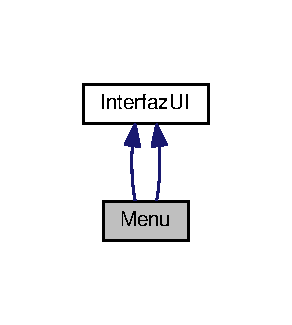
\includegraphics[width=140pt]{class_menu__inherit__graph}
\end{center}
\end{figure}


Collaboration diagram for Menu\+:
\nopagebreak
\begin{figure}[H]
\begin{center}
\leavevmode
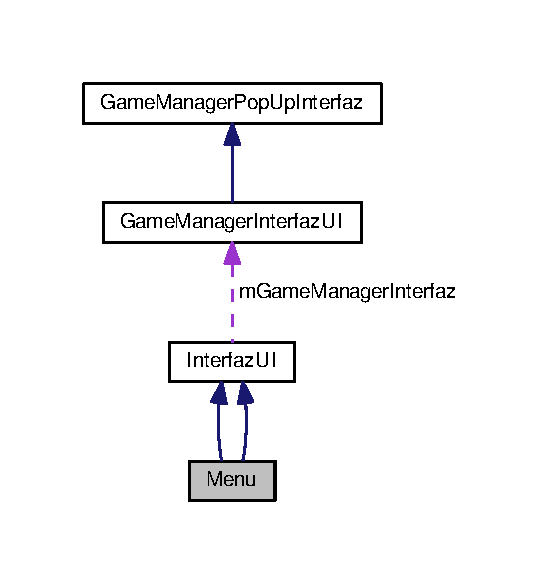
\includegraphics[width=261pt]{class_menu__coll__graph}
\end{center}
\end{figure}
\subsection*{Public Member Functions}
\begin{DoxyCompactItemize}
\item 
{\bfseries Menu} (\hyperlink{class_game_manager_interfaz_u_i}{Game\+Manager\+Interfaz\+UI} $\ast$game\+Manager\+Interfaz)\hypertarget{class_menu_a965ae68f255ca10ec4ed52c3aa0d9188}{}\label{class_menu_a965ae68f255ca10ec4ed52c3aa0d9188}

\item 
void \hyperlink{class_menu_a12119ab1b9abbc5215f6b80be4e3f94b}{prepare} () override
\item 
void \hyperlink{class_menu_a71c36f40cdf039d07172222f4e1c4566}{create\+UI} (S\+D\+L\+\_\+\+Renderer $\ast$g\+Renderer) override
\item 
void \hyperlink{class_menu_ae3d38e9e9b2bfc6a99810fbd178a9f04}{start} () override
\item 
void {\bfseries resume} () override\hypertarget{class_menu_a59f8f24061a98dab9e3a7068bd89180d}{}\label{class_menu_a59f8f24061a98dab9e3a7068bd89180d}

\item 
void {\bfseries procesar\+Evento} (S\+D\+L\+\_\+\+Event $\ast$event) override\hypertarget{class_menu_a4d582e3e75d272369a97d38dd30b2423}{}\label{class_menu_a4d582e3e75d272369a97d38dd30b2423}

\item 
void {\bfseries update} () override\hypertarget{class_menu_a0878f621aa4501fe0e8f388c2222ead6}{}\label{class_menu_a0878f621aa4501fe0e8f388c2222ead6}

\item 
void {\bfseries draw} (S\+D\+L\+\_\+\+Renderer $\ast$g\+Renderer) override\hypertarget{class_menu_a514595f1b580a1787aa20f37f499e68d}{}\label{class_menu_a514595f1b580a1787aa20f37f499e68d}

\item 
{\bfseries Menu} (\hyperlink{class_game_manager_interfaz_u_i}{Game\+Manager\+Interfaz\+UI} $\ast$game\+Manager\+Interfaz)\hypertarget{class_menu_a965ae68f255ca10ec4ed52c3aa0d9188}{}\label{class_menu_a965ae68f255ca10ec4ed52c3aa0d9188}

\item 
void \hyperlink{class_menu_a12119ab1b9abbc5215f6b80be4e3f94b}{prepare} () override
\item 
void \hyperlink{class_menu_a71c36f40cdf039d07172222f4e1c4566}{create\+UI} (S\+D\+L\+\_\+\+Renderer $\ast$g\+Renderer) override
\item 
void \hyperlink{class_menu_ae3d38e9e9b2bfc6a99810fbd178a9f04}{start} () override
\item 
void {\bfseries resume} () override\hypertarget{class_menu_a59f8f24061a98dab9e3a7068bd89180d}{}\label{class_menu_a59f8f24061a98dab9e3a7068bd89180d}

\item 
void {\bfseries procesar\+Evento} (S\+D\+L\+\_\+\+Event $\ast$event) override\hypertarget{class_menu_a4d582e3e75d272369a97d38dd30b2423}{}\label{class_menu_a4d582e3e75d272369a97d38dd30b2423}

\item 
void {\bfseries update} () override\hypertarget{class_menu_a0878f621aa4501fe0e8f388c2222ead6}{}\label{class_menu_a0878f621aa4501fe0e8f388c2222ead6}

\item 
void {\bfseries draw} (S\+D\+L\+\_\+\+Renderer $\ast$g\+Renderer) override\hypertarget{class_menu_a514595f1b580a1787aa20f37f499e68d}{}\label{class_menu_a514595f1b580a1787aa20f37f499e68d}

\end{DoxyCompactItemize}
\subsection*{Additional Inherited Members}


\subsection{Member Function Documentation}
\index{Menu@{Menu}!create\+UI@{create\+UI}}
\index{create\+UI@{create\+UI}!Menu@{Menu}}
\subsubsection[{\texorpdfstring{create\+U\+I(\+S\+D\+L\+\_\+\+Renderer $\ast$g\+Renderer) override}{createUI(SDL_Renderer *gRenderer) override}}]{\setlength{\rightskip}{0pt plus 5cm}void Menu\+::create\+UI (
\begin{DoxyParamCaption}
\item[{S\+D\+L\+\_\+\+Renderer $\ast$}]{g\+Renderer}
\end{DoxyParamCaption}
)\hspace{0.3cm}{\ttfamily [inline]}, {\ttfamily [override]}, {\ttfamily [virtual]}}\hypertarget{class_menu_a71c36f40cdf039d07172222f4e1c4566}{}\label{class_menu_a71c36f40cdf039d07172222f4e1c4566}
Este metodo se encarga de crear la UI necesaria/inicial de la interfaz. En algunos juegos no es necesario establecer UI en este metodo, sino dibujarlo tod cuando se llama a Interfaz\+U\+I\+::draw

Sin embargo, crear los elementos de la UI por adelantado ayuda en la utilización de dirty rects y parecidos. 
\begin{DoxyParams}{Parameters}
{\em g\+Renderer} & \\
\hline
\end{DoxyParams}


Reimplemented from \hyperlink{class_interfaz_u_i_a9dd59265e0790f06862fdfb12494767e}{Interfaz\+UI}.

\index{Menu@{Menu}!create\+UI@{create\+UI}}
\index{create\+UI@{create\+UI}!Menu@{Menu}}
\subsubsection[{\texorpdfstring{create\+U\+I(\+S\+D\+L\+\_\+\+Renderer $\ast$g\+Renderer) override}{createUI(SDL_Renderer *gRenderer) override}}]{\setlength{\rightskip}{0pt plus 5cm}void Menu\+::create\+UI (
\begin{DoxyParamCaption}
\item[{S\+D\+L\+\_\+\+Renderer $\ast$}]{g\+Renderer}
\end{DoxyParamCaption}
)\hspace{0.3cm}{\ttfamily [inline]}, {\ttfamily [override]}, {\ttfamily [virtual]}}\hypertarget{class_menu_a71c36f40cdf039d07172222f4e1c4566}{}\label{class_menu_a71c36f40cdf039d07172222f4e1c4566}
Este metodo se encarga de crear la UI necesaria/inicial de la interfaz. En algunos juegos no es necesario establecer UI en este metodo, sino dibujarlo tod cuando se llama a Interfaz\+U\+I\+::draw

Sin embargo, crear los elementos de la UI por adelantado ayuda en la utilización de dirty rects y parecidos. 
\begin{DoxyParams}{Parameters}
{\em g\+Renderer} & \\
\hline
\end{DoxyParams}


Reimplemented from \hyperlink{class_interfaz_u_i_a9dd59265e0790f06862fdfb12494767e}{Interfaz\+UI}.

\index{Menu@{Menu}!prepare@{prepare}}
\index{prepare@{prepare}!Menu@{Menu}}
\subsubsection[{\texorpdfstring{prepare() override}{prepare() override}}]{\setlength{\rightskip}{0pt plus 5cm}void Menu\+::prepare (
\begin{DoxyParamCaption}
{}
\end{DoxyParamCaption}
)\hspace{0.3cm}{\ttfamily [inline]}, {\ttfamily [override]}, {\ttfamily [virtual]}}\hypertarget{class_menu_a12119ab1b9abbc5215f6b80be4e3f94b}{}\label{class_menu_a12119ab1b9abbc5215f6b80be4e3f94b}
Se encarga de establecer valores de variables iniciales de la Interfaz Este metodo se ejecuta antes de create\+UI, por lo que puede usarse para obtener datos necesarios para la creacion de la UI 

Reimplemented from \hyperlink{class_interfaz_u_i_a312ba3176f7778589cd67f1828682012}{Interfaz\+UI}.

\index{Menu@{Menu}!prepare@{prepare}}
\index{prepare@{prepare}!Menu@{Menu}}
\subsubsection[{\texorpdfstring{prepare() override}{prepare() override}}]{\setlength{\rightskip}{0pt plus 5cm}void Menu\+::prepare (
\begin{DoxyParamCaption}
{}
\end{DoxyParamCaption}
)\hspace{0.3cm}{\ttfamily [inline]}, {\ttfamily [override]}, {\ttfamily [virtual]}}\hypertarget{class_menu_a12119ab1b9abbc5215f6b80be4e3f94b}{}\label{class_menu_a12119ab1b9abbc5215f6b80be4e3f94b}
Se encarga de establecer valores de variables iniciales de la Interfaz Este metodo se ejecuta antes de create\+UI, por lo que puede usarse para obtener datos necesarios para la creacion de la UI 

Reimplemented from \hyperlink{class_interfaz_u_i_a312ba3176f7778589cd67f1828682012}{Interfaz\+UI}.

\index{Menu@{Menu}!start@{start}}
\index{start@{start}!Menu@{Menu}}
\subsubsection[{\texorpdfstring{start() override}{start() override}}]{\setlength{\rightskip}{0pt plus 5cm}void Menu\+::start (
\begin{DoxyParamCaption}
{}
\end{DoxyParamCaption}
)\hspace{0.3cm}{\ttfamily [inline]}, {\ttfamily [override]}, {\ttfamily [virtual]}}\hypertarget{class_menu_ae3d38e9e9b2bfc6a99810fbd178a9f04}{}\label{class_menu_ae3d38e9e9b2bfc6a99810fbd178a9f04}
Este metodo se encarga de Iniciar la Interfaz, al igual que los anteriores métodos. Este metodo debe usarse para dividir el inicio de variables y elementos del juego. 

Reimplemented from \hyperlink{class_interfaz_u_i_a2a80214a4387c21c34a617a8a96996ca}{Interfaz\+UI}.

\index{Menu@{Menu}!start@{start}}
\index{start@{start}!Menu@{Menu}}
\subsubsection[{\texorpdfstring{start() override}{start() override}}]{\setlength{\rightskip}{0pt plus 5cm}void Menu\+::start (
\begin{DoxyParamCaption}
{}
\end{DoxyParamCaption}
)\hspace{0.3cm}{\ttfamily [inline]}, {\ttfamily [override]}, {\ttfamily [virtual]}}\hypertarget{class_menu_ae3d38e9e9b2bfc6a99810fbd178a9f04}{}\label{class_menu_ae3d38e9e9b2bfc6a99810fbd178a9f04}
Este metodo se encarga de Iniciar la Interfaz, al igual que los anteriores métodos. Este metodo debe usarse para dividir el inicio de variables y elementos del juego. 

Reimplemented from \hyperlink{class_interfaz_u_i_a2a80214a4387c21c34a617a8a96996ca}{Interfaz\+UI}.



The documentation for this class was generated from the following file\+:\begin{DoxyCompactItemize}
\item 
src/testsotrosjuegos/\+Othello/Menu.\+hpp\end{DoxyCompactItemize}

\hypertarget{class_menu_list_label}{}\section{Menu\+List\+Label Class Reference}
\label{class_menu_list_label}\index{Menu\+List\+Label@{Menu\+List\+Label}}


Inheritance diagram for Menu\+List\+Label\+:\nopagebreak
\begin{figure}[H]
\begin{center}
\leavevmode
\includegraphics[width=272pt]{class_menu_list_label__inherit__graph}
\end{center}
\end{figure}


Collaboration diagram for Menu\+List\+Label\+:
\nopagebreak
\begin{figure}[H]
\begin{center}
\leavevmode
\includegraphics[width=350pt]{class_menu_list_label__coll__graph}
\end{center}
\end{figure}
\subsection*{Public Member Functions}
\begin{DoxyCompactItemize}
\item 
{\bfseries Menu\+List\+Label} (\hyperlink{class_game_manager_interfaz_u_i}{Game\+Manager\+Interfaz\+UI} $\ast$game\+Manager\+Interfaz)\hypertarget{class_menu_list_label_a1b63e875b7833876e771ea0bb09b56ba}{}\label{class_menu_list_label_a1b63e875b7833876e771ea0bb09b56ba}

\item 
void \hyperlink{class_menu_list_label_aaa91bf445c3db2fa2008a06b5e96df24}{prepare} () override
\item 
virtual void \hyperlink{class_menu_list_label_aa4622ae2bc0bf7d31aa8fe8483103e27}{create\+UI} (S\+D\+L\+\_\+\+Renderer $\ast$renderer) override
\item 
virtual void {\bfseries resume} () override\hypertarget{class_menu_list_label_adf653340269ada2e89b343ce37669d7d}{}\label{class_menu_list_label_adf653340269ada2e89b343ce37669d7d}

\item 
virtual bool \hyperlink{class_menu_list_label_aa4b43b15d99168836a26ce8e9cf996a6}{set\+Opcion\+Resaltada} (int nueva\+Opcion)
\item 
virtual void {\bfseries ejecutar\+Accion\+Opcion\+Resaltada} ()=0\hypertarget{class_menu_list_label_ab24db858c8bec69186a40b10670ac752}{}\label{class_menu_list_label_ab24db858c8bec69186a40b10670ac752}

\item 
void \hyperlink{class_menu_list_label_a7fb1ac75f91fe00f38706f74f6148cd6}{procesar\+Evento} (S\+D\+L\+\_\+\+Event $\ast$evento) override
\item 
void {\bfseries draw} (S\+D\+L\+\_\+\+Renderer $\ast$renderer) override\hypertarget{class_menu_list_label_a5fb48d986e1ea0f85428d3f52e98ef57}{}\label{class_menu_list_label_a5fb48d986e1ea0f85428d3f52e98ef57}

\end{DoxyCompactItemize}
\subsection*{Protected Attributes}
\begin{DoxyCompactItemize}
\item 
deque$<$ \hyperlink{class_label_component}{Label\+Component} $\ast$ $>$ {\bfseries menu\+Text\+Options}\hypertarget{class_menu_list_label_a4d0a9e5581aa3ebf2d6d5599fdb2dfed}{}\label{class_menu_list_label_a4d0a9e5581aa3ebf2d6d5599fdb2dfed}

\item 
\hyperlink{class_layout_vertical}{Layout\+Vertical} $\ast$ {\bfseries m\+Layout} = nullptr\hypertarget{class_menu_list_label_a78112edcf4dccb025b60192373bc5b8e}{}\label{class_menu_list_label_a78112edcf4dccb025b60192373bc5b8e}

\item 
\hyperlink{class_layout_vertical}{Layout\+Vertical} $\ast$ {\bfseries m\+Layout\+Back\+Ground} = nullptr\hypertarget{class_menu_list_label_a00a12da8ca12067b9e46ee47df4ddb37}{}\label{class_menu_list_label_a00a12da8ca12067b9e46ee47df4ddb37}

\item 
deque$<$ string $>$ {\bfseries m\+Menu\+Opciones\+Text}\hypertarget{class_menu_list_label_a8069cc9a24b9151931c6d7ceb5774c59}{}\label{class_menu_list_label_a8069cc9a24b9151931c6d7ceb5774c59}

\item 
S\+D\+L\+\_\+\+Color {\bfseries m\+Color\+Label\+Normal} \{255,0,0,255\}\hypertarget{class_menu_list_label_a60ca7a85009c7c1eaee487a949db8ff8}{}\label{class_menu_list_label_a60ca7a85009c7c1eaee487a949db8ff8}

\item 
S\+D\+L\+\_\+\+Color {\bfseries m\+Color\+Label\+Resaltado} \{255,255,0,255\}\hypertarget{class_menu_list_label_a75f5e912229d412283d2e8b47b6c658a}{}\label{class_menu_list_label_a75f5e912229d412283d2e8b47b6c658a}

\item 
int {\bfseries m\+Opcion\+Menu\+Resaltada\+Actual} = -\/1\hypertarget{class_menu_list_label_a5ae196badf289099b400dad5a89eaa34}{}\label{class_menu_list_label_a5ae196badf289099b400dad5a89eaa34}

\end{DoxyCompactItemize}


\subsection{Detailed Description}
\begin{Desc}
\item[Examples\+: ]\par
\hyperlink{_2home_2manuggz_2_documents_2_projects_2_bomberman_2src_2engine_2interfaces_2_menu_list_label_8hpp-example}{/home/manuggz/\+Documents/\+Projects/\+Bomberman/src/engine/interfaces/\+Menu\+List\+Label.\+hpp}.\end{Desc}


\subsection{Member Function Documentation}
\index{Menu\+List\+Label@{Menu\+List\+Label}!create\+UI@{create\+UI}}
\index{create\+UI@{create\+UI}!Menu\+List\+Label@{Menu\+List\+Label}}
\subsubsection[{\texorpdfstring{create\+U\+I(\+S\+D\+L\+\_\+\+Renderer $\ast$renderer) override}{createUI(SDL_Renderer *renderer) override}}]{\setlength{\rightskip}{0pt plus 5cm}virtual void Menu\+List\+Label\+::create\+UI (
\begin{DoxyParamCaption}
\item[{S\+D\+L\+\_\+\+Renderer $\ast$}]{g\+Renderer}
\end{DoxyParamCaption}
)\hspace{0.3cm}{\ttfamily [inline]}, {\ttfamily [override]}, {\ttfamily [virtual]}}\hypertarget{class_menu_list_label_aa4622ae2bc0bf7d31aa8fe8483103e27}{}\label{class_menu_list_label_aa4622ae2bc0bf7d31aa8fe8483103e27}
Este metodo se encarga de crear la UI necesaria/inicial de la interfaz. En algunos juegos no es necesario establecer UI en este metodo, sino dibujarlo tod cuando se llama a Interfaz\+U\+I\+::draw

Sin embargo, crear los elementos de la UI por adelantado ayuda en la utilización de dirty rects y parecidos. 
\begin{DoxyParams}{Parameters}
{\em g\+Renderer} & \\
\hline
\end{DoxyParams}


Reimplemented from \hyperlink{class_interfaz_u_i_a9dd59265e0790f06862fdfb12494767e}{Interfaz\+UI}.

\begin{Desc}
\item[Examples\+: ]\par
\hyperlink{_2home_2manuggz_2_documents_2_projects_2_bomberman_2src_2engine_2interfaces_2_menu_list_label_8hpp-example}{/home/manuggz/\+Documents/\+Projects/\+Bomberman/src/engine/interfaces/\+Menu\+List\+Label.\+hpp}.\end{Desc}
\index{Menu\+List\+Label@{Menu\+List\+Label}!prepare@{prepare}}
\index{prepare@{prepare}!Menu\+List\+Label@{Menu\+List\+Label}}
\subsubsection[{\texorpdfstring{prepare() override}{prepare() override}}]{\setlength{\rightskip}{0pt plus 5cm}void Menu\+List\+Label\+::prepare (
\begin{DoxyParamCaption}
{}
\end{DoxyParamCaption}
)\hspace{0.3cm}{\ttfamily [inline]}, {\ttfamily [override]}, {\ttfamily [virtual]}}\hypertarget{class_menu_list_label_aaa91bf445c3db2fa2008a06b5e96df24}{}\label{class_menu_list_label_aaa91bf445c3db2fa2008a06b5e96df24}
Se encarga de establecer valores de variables iniciales de la Interfaz Este metodo se ejecuta antes de create\+UI, por lo que puede usarse para obtener datos necesarios para la creacion de la UI 

Reimplemented from \hyperlink{class_interfaz_u_i_a312ba3176f7778589cd67f1828682012}{Interfaz\+UI}.

\begin{Desc}
\item[Examples\+: ]\par
\hyperlink{_2home_2manuggz_2_documents_2_projects_2_bomberman_2src_2engine_2interfaces_2_menu_list_label_8hpp-example}{/home/manuggz/\+Documents/\+Projects/\+Bomberman/src/engine/interfaces/\+Menu\+List\+Label.\+hpp}.\end{Desc}
\index{Menu\+List\+Label@{Menu\+List\+Label}!procesar\+Evento@{procesar\+Evento}}
\index{procesar\+Evento@{procesar\+Evento}!Menu\+List\+Label@{Menu\+List\+Label}}
\subsubsection[{\texorpdfstring{procesar\+Evento(\+S\+D\+L\+\_\+\+Event $\ast$evento) override}{procesarEvento(SDL_Event *evento) override}}]{\setlength{\rightskip}{0pt plus 5cm}void Menu\+List\+Label\+::procesar\+Evento (
\begin{DoxyParamCaption}
\item[{S\+D\+L\+\_\+\+Event $\ast$}]{evento}
\end{DoxyParamCaption}
)\hspace{0.3cm}{\ttfamily [inline]}, {\ttfamily [override]}, {\ttfamily [virtual]}}\hypertarget{class_menu_list_label_a7fb1ac75f91fe00f38706f74f6148cd6}{}\label{class_menu_list_label_a7fb1ac75f91fe00f38706f74f6148cd6}
Procesa el evento del usuario Se encarga de mover la opcion resaltada al usuario o en caso de que sea E\+N\+T\+ER llamar a la funcion enlazada a la opcion. 
\begin{DoxyParams}{Parameters}
{\em evento} & Evento producido por S\+DL \\
\hline
\end{DoxyParams}


Reimplemented from \hyperlink{class_interfaz_u_i}{Interfaz\+UI}.

\begin{Desc}
\item[Examples\+: ]\par
\hyperlink{_2home_2manuggz_2_documents_2_projects_2_bomberman_2src_2engine_2interfaces_2_menu_list_label_8hpp-example}{/home/manuggz/\+Documents/\+Projects/\+Bomberman/src/engine/interfaces/\+Menu\+List\+Label.\+hpp}.\end{Desc}
\index{Menu\+List\+Label@{Menu\+List\+Label}!set\+Opcion\+Resaltada@{set\+Opcion\+Resaltada}}
\index{set\+Opcion\+Resaltada@{set\+Opcion\+Resaltada}!Menu\+List\+Label@{Menu\+List\+Label}}
\subsubsection[{\texorpdfstring{set\+Opcion\+Resaltada(int nueva\+Opcion)}{setOpcionResaltada(int nuevaOpcion)}}]{\setlength{\rightskip}{0pt plus 5cm}virtual bool Menu\+List\+Label\+::set\+Opcion\+Resaltada (
\begin{DoxyParamCaption}
\item[{int}]{nueva\+Opcion}
\end{DoxyParamCaption}
)\hspace{0.3cm}{\ttfamily [inline]}, {\ttfamily [virtual]}}\hypertarget{class_menu_list_label_aa4b43b15d99168836a26ce8e9cf996a6}{}\label{class_menu_list_label_aa4b43b15d99168836a26ce8e9cf996a6}
Establece la nueva opcion del menu resaltada al usuario 
\begin{DoxyParams}{Parameters}
{\em nueva\+Opcion} & Nueva seleccion \\
\hline
\end{DoxyParams}
\begin{DoxyReturn}{Returns}
True en caso que se haya resaltado con exito, false en caso contrario 
\end{DoxyReturn}


Reimplemented in \hyperlink{class_menu_principal_a8870a656a23920c518bc2fbdf7c72a53}{Menu\+Principal}.

\begin{Desc}
\item[Examples\+: ]\par
\hyperlink{_2home_2manuggz_2_documents_2_projects_2_bomberman_2src_2engine_2interfaces_2_menu_list_label_8hpp-example}{/home/manuggz/\+Documents/\+Projects/\+Bomberman/src/engine/interfaces/\+Menu\+List\+Label.\+hpp}.\end{Desc}


The documentation for this class was generated from the following file\+:\begin{DoxyCompactItemize}
\item 
src/engine/interfaces/Menu\+List\+Label.\+hpp\end{DoxyCompactItemize}

\hypertarget{class_menu_modo_multijugador}{}\section{Menu\+Modo\+Multijugador Class Reference}
\label{class_menu_modo_multijugador}\index{Menu\+Modo\+Multijugador@{Menu\+Modo\+Multijugador}}


Inheritance diagram for Menu\+Modo\+Multijugador\+:\nopagebreak
\begin{figure}[H]
\begin{center}
\leavevmode
\includegraphics[width=260pt]{class_menu_modo_multijugador__inherit__graph}
\end{center}
\end{figure}


Collaboration diagram for Menu\+Modo\+Multijugador\+:\nopagebreak
\begin{figure}[H]
\begin{center}
\leavevmode
\includegraphics[width=301pt]{class_menu_modo_multijugador__coll__graph}
\end{center}
\end{figure}
\subsection*{Public Member Functions}
\begin{DoxyCompactItemize}
\item 
{\bfseries Menu\+Modo\+Multijugador} (\hyperlink{class_game_manager_interfaz_u_i}{Game\+Manager\+Interfaz\+UI} $\ast$game\+Manager\+Interfaz\+UI)\hypertarget{class_menu_modo_multijugador_aa9376a8627b1b6bd15beecc392fe3721}{}\label{class_menu_modo_multijugador_aa9376a8627b1b6bd15beecc392fe3721}

\item 
void \hyperlink{class_menu_modo_multijugador_a422baa9893784cacd414b13fbd34e7d2}{prepare} () override
\item 
void \hyperlink{class_menu_modo_multijugador_aa87c06427be64fd73e17d9ea37d8744e}{create\+UI} (S\+D\+L\+\_\+\+Renderer $\ast$g\+Renderer) override
\item 
virtual void \hyperlink{class_menu_modo_multijugador_a0957d2b62ca4851a3a868403767c9d61}{eliminar\+Sprite} (\hyperlink{class_sprite}{Sprite} $\ast$sprite) override
\item 
void {\bfseries pack\+Layout} (S\+D\+L\+\_\+\+Renderer $\ast$g\+Renderer)\hypertarget{class_menu_modo_multijugador_a2a13518afeedfeab61b030c376ee35e2}{}\label{class_menu_modo_multijugador_a2a13518afeedfeab61b030c376ee35e2}

\item 
bool \hyperlink{class_menu_modo_multijugador_a77f0be9bcdc3fbdf3130a024ef25bef5}{establecer\+Terreno\+Batalla} (S\+D\+L\+\_\+\+Renderer $\ast$g\+Renderer, int nuevo\+Terreno)
\item 
void \hyperlink{class_menu_modo_multijugador_a3aee7e0e5ab94f1e866f9306aabed208}{click\+Control} (\hyperlink{class_boton_component}{Boton\+Component}$<$ \hyperlink{class_menu_modo_multijugador}{Menu\+Modo\+Multijugador} $>$ $\ast$control\+\_\+click)
\item 
void \hyperlink{class_menu_modo_multijugador_a589a0611b7f3cf2978ff1ab72ce3b35c}{ejecutar\+Accion\+Boton\+Clicked} ()
\item 
void \hyperlink{class_menu_modo_multijugador_a6e483dbb12275b6e00be0f9fb430dd7e}{cambiar\+Estado\+Player} (int id\+Player)
\item 
virtual void {\bfseries resume} () override\hypertarget{class_menu_modo_multijugador_a61af68ebd0132c9ee7fc4c505e2befa0}{}\label{class_menu_modo_multijugador_a61af68ebd0132c9ee7fc4c505e2befa0}

\item 
virtual void {\bfseries procesar\+Evento} (S\+D\+L\+\_\+\+Event $\ast$event) override\hypertarget{class_menu_modo_multijugador_a6520fcac1cc0bff79f00c509e34afbd0}{}\label{class_menu_modo_multijugador_a6520fcac1cc0bff79f00c509e34afbd0}

\item 
virtual void {\bfseries update} () override\hypertarget{class_menu_modo_multijugador_ac2ec2a9594a2637b15e43477d2e10f07}{}\label{class_menu_modo_multijugador_ac2ec2a9594a2637b15e43477d2e10f07}

\item 
virtual void {\bfseries draw} (S\+D\+L\+\_\+\+Renderer $\ast$g\+Renderer) override\hypertarget{class_menu_modo_multijugador_a1c4c4196780896d241ceaa6f696bc179}{}\label{class_menu_modo_multijugador_a1c4c4196780896d241ceaa6f696bc179}

\end{DoxyCompactItemize}
\subsection*{Additional Inherited Members}


\subsection{Member Function Documentation}
\index{Menu\+Modo\+Multijugador@{Menu\+Modo\+Multijugador}!cambiar\+Estado\+Player@{cambiar\+Estado\+Player}}
\index{cambiar\+Estado\+Player@{cambiar\+Estado\+Player}!Menu\+Modo\+Multijugador@{Menu\+Modo\+Multijugador}}
\subsubsection[{\texorpdfstring{cambiar\+Estado\+Player(int id\+Player)}{cambiarEstadoPlayer(int idPlayer)}}]{\setlength{\rightskip}{0pt plus 5cm}void Menu\+Modo\+Multijugador\+::cambiar\+Estado\+Player (
\begin{DoxyParamCaption}
\item[{int}]{id\+Player}
\end{DoxyParamCaption}
)\hspace{0.3cm}{\ttfamily [inline]}}\hypertarget{class_menu_modo_multijugador_a6e483dbb12275b6e00be0f9fb430dd7e}{}\label{class_menu_modo_multijugador_a6e483dbb12275b6e00be0f9fb430dd7e}
Cambia el estado de un player lo establece activo/desactivado 
\begin{DoxyParams}{Parameters}
{\em id\+Player} & \\
\hline
\end{DoxyParams}
\index{Menu\+Modo\+Multijugador@{Menu\+Modo\+Multijugador}!click\+Control@{click\+Control}}
\index{click\+Control@{click\+Control}!Menu\+Modo\+Multijugador@{Menu\+Modo\+Multijugador}}
\subsubsection[{\texorpdfstring{click\+Control(\+Boton\+Component$<$ Menu\+Modo\+Multijugador $>$ $\ast$control\+\_\+click)}{clickControl(BotonComponent< MenuModoMultijugador > *control_click)}}]{\setlength{\rightskip}{0pt plus 5cm}void Menu\+Modo\+Multijugador\+::click\+Control (
\begin{DoxyParamCaption}
\item[{{\bf Boton\+Component}$<$ {\bf Menu\+Modo\+Multijugador} $>$ $\ast$}]{control\+\_\+click}
\end{DoxyParamCaption}
)\hspace{0.3cm}{\ttfamily [inline]}}\hypertarget{class_menu_modo_multijugador_a3aee7e0e5ab94f1e866f9306aabed208}{}\label{class_menu_modo_multijugador_a3aee7e0e5ab94f1e866f9306aabed208}
Funcion llamada por los botones de la interfaz cuando son presionados 
\begin{DoxyParams}{Parameters}
{\em control\+\_\+click} & \\
\hline
\end{DoxyParams}
\index{Menu\+Modo\+Multijugador@{Menu\+Modo\+Multijugador}!create\+UI@{create\+UI}}
\index{create\+UI@{create\+UI}!Menu\+Modo\+Multijugador@{Menu\+Modo\+Multijugador}}
\subsubsection[{\texorpdfstring{create\+U\+I(\+S\+D\+L\+\_\+\+Renderer $\ast$g\+Renderer) override}{createUI(SDL_Renderer *gRenderer) override}}]{\setlength{\rightskip}{0pt plus 5cm}void Menu\+Modo\+Multijugador\+::create\+UI (
\begin{DoxyParamCaption}
\item[{S\+D\+L\+\_\+\+Renderer $\ast$}]{g\+Renderer}
\end{DoxyParamCaption}
)\hspace{0.3cm}{\ttfamily [inline]}, {\ttfamily [override]}, {\ttfamily [virtual]}}\hypertarget{class_menu_modo_multijugador_aa87c06427be64fd73e17d9ea37d8744e}{}\label{class_menu_modo_multijugador_aa87c06427be64fd73e17d9ea37d8744e}
Este metodo se encarga de crear la UI necesaria/inicial de la interfaz. En algunos juegos no es necesario establecer UI en este metodo, sino dibujarlo tod cuando se llama a Interfaz\+U\+I\+::draw

Sin embargo, crear los elementos de la UI por adelantado ayuda en la utilización de dirty rects y parecidos. 
\begin{DoxyParams}{Parameters}
{\em g\+Renderer} & \\
\hline
\end{DoxyParams}


Reimplemented from \hyperlink{class_interfaz_u_i_a9dd59265e0790f06862fdfb12494767e}{Interfaz\+UI}.

\index{Menu\+Modo\+Multijugador@{Menu\+Modo\+Multijugador}!ejecutar\+Accion\+Boton\+Clicked@{ejecutar\+Accion\+Boton\+Clicked}}
\index{ejecutar\+Accion\+Boton\+Clicked@{ejecutar\+Accion\+Boton\+Clicked}!Menu\+Modo\+Multijugador@{Menu\+Modo\+Multijugador}}
\subsubsection[{\texorpdfstring{ejecutar\+Accion\+Boton\+Clicked()}{ejecutarAccionBotonClicked()}}]{\setlength{\rightskip}{0pt plus 5cm}void Menu\+Modo\+Multijugador\+::ejecutar\+Accion\+Boton\+Clicked (
\begin{DoxyParamCaption}
{}
\end{DoxyParamCaption}
)\hspace{0.3cm}{\ttfamily [inline]}}\hypertarget{class_menu_modo_multijugador_a589a0611b7f3cf2978ff1ab72ce3b35c}{}\label{class_menu_modo_multijugador_a589a0611b7f3cf2978ff1ab72ce3b35c}
Ejecuta la opcion enlazada a un boton \index{Menu\+Modo\+Multijugador@{Menu\+Modo\+Multijugador}!eliminar\+Sprite@{eliminar\+Sprite}}
\index{eliminar\+Sprite@{eliminar\+Sprite}!Menu\+Modo\+Multijugador@{Menu\+Modo\+Multijugador}}
\subsubsection[{\texorpdfstring{eliminar\+Sprite(\+Sprite $\ast$sprite) override}{eliminarSprite(Sprite *sprite) override}}]{\setlength{\rightskip}{0pt plus 5cm}virtual void Menu\+Modo\+Multijugador\+::eliminar\+Sprite (
\begin{DoxyParamCaption}
\item[{{\bf Sprite} $\ast$}]{}
\end{DoxyParamCaption}
)\hspace{0.3cm}{\ttfamily [inline]}, {\ttfamily [override]}, {\ttfamily [virtual]}}\hypertarget{class_menu_modo_multijugador_a0957d2b62ca4851a3a868403767c9d61}{}\label{class_menu_modo_multijugador_a0957d2b62ca4851a3a868403767c9d61}
Elimina un \hyperlink{class_sprite}{Sprite} de Memoria. Esta función es llamada desde un Update\+Group/\+Derivado cuando se elimina un \hyperlink{class_sprite}{Sprite} con kill(). 

Implements \hyperlink{class_interfaz_sprite_group_acad50741e8bab94e3ce1f8c4c0cbad52}{Interfaz\+Sprite\+Group}.

\index{Menu\+Modo\+Multijugador@{Menu\+Modo\+Multijugador}!establecer\+Terreno\+Batalla@{establecer\+Terreno\+Batalla}}
\index{establecer\+Terreno\+Batalla@{establecer\+Terreno\+Batalla}!Menu\+Modo\+Multijugador@{Menu\+Modo\+Multijugador}}
\subsubsection[{\texorpdfstring{establecer\+Terreno\+Batalla(\+S\+D\+L\+\_\+\+Renderer $\ast$g\+Renderer, int nuevo\+Terreno)}{establecerTerrenoBatalla(SDL_Renderer *gRenderer, int nuevoTerreno)}}]{\setlength{\rightskip}{0pt plus 5cm}bool Menu\+Modo\+Multijugador\+::establecer\+Terreno\+Batalla (
\begin{DoxyParamCaption}
\item[{S\+D\+L\+\_\+\+Renderer $\ast$}]{g\+Renderer, }
\item[{int}]{nuevo\+Terreno}
\end{DoxyParamCaption}
)\hspace{0.3cm}{\ttfamily [inline]}}\hypertarget{class_menu_modo_multijugador_a77f0be9bcdc3fbdf3130a024ef25bef5}{}\label{class_menu_modo_multijugador_a77f0be9bcdc3fbdf3130a024ef25bef5}
Establece/\+Cambia el terreno en el que se jugara 
\begin{DoxyParams}{Parameters}
{\em nuevo\+Terreno} & \\
\hline
\end{DoxyParams}
\begin{DoxyReturn}{Returns}

\end{DoxyReturn}
\index{Menu\+Modo\+Multijugador@{Menu\+Modo\+Multijugador}!prepare@{prepare}}
\index{prepare@{prepare}!Menu\+Modo\+Multijugador@{Menu\+Modo\+Multijugador}}
\subsubsection[{\texorpdfstring{prepare() override}{prepare() override}}]{\setlength{\rightskip}{0pt plus 5cm}void Menu\+Modo\+Multijugador\+::prepare (
\begin{DoxyParamCaption}
{}
\end{DoxyParamCaption}
)\hspace{0.3cm}{\ttfamily [inline]}, {\ttfamily [override]}, {\ttfamily [virtual]}}\hypertarget{class_menu_modo_multijugador_a422baa9893784cacd414b13fbd34e7d2}{}\label{class_menu_modo_multijugador_a422baa9893784cacd414b13fbd34e7d2}
Se encarga de establecer valores de variables iniciales de la Interfaz Este metodo se ejecuta antes de create\+UI, por lo que puede usarse para obtener datos necesarios para la creacion de la UI 

Reimplemented from \hyperlink{class_interfaz_u_i_a312ba3176f7778589cd67f1828682012}{Interfaz\+UI}.



The documentation for this class was generated from the following file\+:\begin{DoxyCompactItemize}
\item 
src/\+Interfaces/menu/Menu\+Modo\+Multijugador.\+hpp\end{DoxyCompactItemize}

\hypertarget{class_menu_nuevo_juego}{}\section{Menu\+Nuevo\+Juego Class Reference}
\label{class_menu_nuevo_juego}\index{Menu\+Nuevo\+Juego@{Menu\+Nuevo\+Juego}}


Inheritance diagram for Menu\+Nuevo\+Juego\+:\nopagebreak
\begin{figure}[H]
\begin{center}
\leavevmode
\includegraphics[width=175pt]{class_menu_nuevo_juego__inherit__graph}
\end{center}
\end{figure}


Collaboration diagram for Menu\+Nuevo\+Juego\+:
\nopagebreak
\begin{figure}[H]
\begin{center}
\leavevmode
\includegraphics[width=350pt]{class_menu_nuevo_juego__coll__graph}
\end{center}
\end{figure}
\subsection*{Public Member Functions}
\begin{DoxyCompactItemize}
\item 
{\bfseries Menu\+Nuevo\+Juego} (\hyperlink{class_game_manager_interfaz_u_i}{Game\+Manager\+Interfaz\+UI} $\ast$game)\hypertarget{class_menu_nuevo_juego_aadb15d1ac9e2ba945802379dd31a4e60}{}\label{class_menu_nuevo_juego_aadb15d1ac9e2ba945802379dd31a4e60}

\item 
void {\bfseries ejecutar\+Accion\+Opcion\+Resaltada} ()\hypertarget{class_menu_nuevo_juego_a2f90015753cd1e839a5cf5e418b28277}{}\label{class_menu_nuevo_juego_a2f90015753cd1e839a5cf5e418b28277}

\end{DoxyCompactItemize}
\subsection*{Additional Inherited Members}


The documentation for this class was generated from the following file\+:\begin{DoxyCompactItemize}
\item 
src/\+Interfaces/menu/Menu\+Nuevo\+Juego.\+hpp\end{DoxyCompactItemize}

\hypertarget{class_menu_principal}{}\section{Menu\+Principal Class Reference}
\label{class_menu_principal}\index{Menu\+Principal@{Menu\+Principal}}


Inheritance diagram for Menu\+Principal\+:\nopagebreak
\begin{figure}[H]
\begin{center}
\leavevmode
\includegraphics[width=160pt]{class_menu_principal__inherit__graph}
\end{center}
\end{figure}


Collaboration diagram for Menu\+Principal\+:
\nopagebreak
\begin{figure}[H]
\begin{center}
\leavevmode
\includegraphics[width=350pt]{class_menu_principal__coll__graph}
\end{center}
\end{figure}
\subsection*{Public Member Functions}
\begin{DoxyCompactItemize}
\item 
{\bfseries Menu\+Principal} (\hyperlink{class_game_manager_interfaz_u_i}{Game\+Manager\+Interfaz\+UI} $\ast$game\+Manager)\hypertarget{class_menu_principal_ac57e54767aafc7c0b9d243ec94026118}{}\label{class_menu_principal_ac57e54767aafc7c0b9d243ec94026118}

\item 
virtual bool \hyperlink{class_menu_principal_a8870a656a23920c518bc2fbdf7c72a53}{set\+Opcion\+Resaltada} (int nueva\+Opcion) override
\item 
void {\bfseries ejecutar\+Accion\+Opcion\+Resaltada} ()\hypertarget{class_menu_principal_a29625ddda752b38c23ee7cc52a77e9b0}{}\label{class_menu_principal_a29625ddda752b38c23ee7cc52a77e9b0}

\end{DoxyCompactItemize}
\subsection*{Additional Inherited Members}


\subsection{Member Function Documentation}
\index{Menu\+Principal@{Menu\+Principal}!set\+Opcion\+Resaltada@{set\+Opcion\+Resaltada}}
\index{set\+Opcion\+Resaltada@{set\+Opcion\+Resaltada}!Menu\+Principal@{Menu\+Principal}}
\subsubsection[{\texorpdfstring{set\+Opcion\+Resaltada(int nueva\+Opcion) override}{setOpcionResaltada(int nuevaOpcion) override}}]{\setlength{\rightskip}{0pt plus 5cm}virtual bool Menu\+Principal\+::set\+Opcion\+Resaltada (
\begin{DoxyParamCaption}
\item[{int}]{nueva\+Opcion}
\end{DoxyParamCaption}
)\hspace{0.3cm}{\ttfamily [inline]}, {\ttfamily [override]}, {\ttfamily [virtual]}}\hypertarget{class_menu_principal_a8870a656a23920c518bc2fbdf7c72a53}{}\label{class_menu_principal_a8870a656a23920c518bc2fbdf7c72a53}
Establece la nueva opcion del menu resaltada al usuario 
\begin{DoxyParams}{Parameters}
{\em nueva\+Opcion} & Nueva seleccion \\
\hline
\end{DoxyParams}
\begin{DoxyReturn}{Returns}
True en caso que se haya resaltado con exito, false en caso contrario 
\end{DoxyReturn}


Reimplemented from \hyperlink{class_menu_list_label_aa4b43b15d99168836a26ce8e9cf996a6}{Menu\+List\+Label}.



The documentation for this class was generated from the following file\+:\begin{DoxyCompactItemize}
\item 
src/\+Interfaces/menu/Menu\+Principal.\+hpp\end{DoxyCompactItemize}

\hypertarget{class_meta_data}{}\section{Meta\+Data Class Reference}
\label{class_meta_data}\index{Meta\+Data@{Meta\+Data}}
\subsection*{Public Member Functions}
\begin{DoxyCompactItemize}
\item 
\hyperlink{class_meta_data_a248c7fa5fa7a913d74082bfff2b54605}{Meta\+Data} (std\+::string ruta, std\+::string delim)
\item 
void \hyperlink{class_meta_data_a316a360f75e55ab4b89afa21a41aad21}{set\+Meta\+Data} (std\+::string clave, std\+::string)
\item 
bool \hyperlink{class_meta_data_a82c33cc7ed0a99536dac97fee486790a}{guardar} (std\+::string ruta\+Destino=\char`\"{}\char`\"{}, std\+::string delimitador=\char`\"{}\+:\char`\"{})
\item 
std\+::string \hyperlink{class_meta_data_a51890f104186763e40e5fa9b98a40c93}{get\+Meta\+Data} (std\+::string clave)
\item 
bool \hyperlink{class_meta_data_a9a7ddd822ce2ccefe542a19b5a84e1e2}{cargar\+Meta\+Data} (std\+::string ruta, std\+::string delim)
\end{DoxyCompactItemize}


\subsection{Constructor \& Destructor Documentation}
\index{Meta\+Data@{Meta\+Data}!Meta\+Data@{Meta\+Data}}
\index{Meta\+Data@{Meta\+Data}!Meta\+Data@{Meta\+Data}}
\subsubsection[{\texorpdfstring{Meta\+Data(std\+::string ruta, std\+::string delim)}{MetaData(std::string ruta, std::string delim)}}]{\setlength{\rightskip}{0pt plus 5cm}Meta\+Data\+::\+Meta\+Data (
\begin{DoxyParamCaption}
\item[{std\+::string}]{ruta, }
\item[{std\+::string}]{delim}
\end{DoxyParamCaption}
)}\hypertarget{class_meta_data_a248c7fa5fa7a913d74082bfff2b54605}{}\label{class_meta_data_a248c7fa5fa7a913d74082bfff2b54605}
Inicializa la clase parseando los datos en un archivo Los datos del archivo deben estar en el siguiente formato

cada linea debe ser de la forma\+:

\mbox{[}$<$key$>$$<$delimitador$>$

\mbox{]} .... \mbox{[}$<$key$>$$<$delimitador$>$

\mbox{]}

Ejemplo\+:

variable1\+:valor1 Variable2\+:valor2


\begin{DoxyParams}{Parameters}
{\em ruta} & \\
\hline
{\em delim} & \\
\hline
\end{DoxyParams}
\begin{DoxyReturn}{Returns}

\end{DoxyReturn}
\begin{DoxyWarning}{Warning}
Notar que no hay espacios en el formato esto es importante porque no se hace trim en la lectura y se toma tod lo que este antes del delimitador como la clave y lo que este despues como el valor incluyendo los espacios. Las lineas donde no se encuentren los delimitadores o n haya clave son ignoradas. Distingue entre mayusculas y minusculas. las claves deben ser unicas. 
\end{DoxyWarning}


\subsection{Member Function Documentation}
\index{Meta\+Data@{Meta\+Data}!cargar\+Meta\+Data@{cargar\+Meta\+Data}}
\index{cargar\+Meta\+Data@{cargar\+Meta\+Data}!Meta\+Data@{Meta\+Data}}
\subsubsection[{\texorpdfstring{cargar\+Meta\+Data(std\+::string ruta, std\+::string delim)}{cargarMetaData(std::string ruta, std::string delim)}}]{\setlength{\rightskip}{0pt plus 5cm}bool Meta\+Data\+::cargar\+Meta\+Data (
\begin{DoxyParamCaption}
\item[{std\+::string}]{ruta, }
\item[{std\+::string}]{delim}
\end{DoxyParamCaption}
)}\hypertarget{class_meta_data_a9a7ddd822ce2ccefe542a19b5a84e1e2}{}\label{class_meta_data_a9a7ddd822ce2ccefe542a19b5a84e1e2}
Inicializa la clase parseando los datos en un archivo Los datos del archivo deben estar en el siguiente formato

cada linea debe ser de la forma\+:

\mbox{[}$<$key$>$$<$delimitador$>$

\mbox{]} .... \mbox{[}$<$key$>$$<$delimitador$>$

\mbox{]}

Ejemplo\+:

variable1\+:valor1 Variable2\+:valor2


\begin{DoxyParams}{Parameters}
{\em ruta} & \\
\hline
{\em delim} & \\
\hline
\end{DoxyParams}
\begin{DoxyReturn}{Returns}

\end{DoxyReturn}
\begin{DoxyWarning}{Warning}
Notar que no hay espacios en el formato esto es importante porque no se hace trim en la lectura y se toma tod lo que este antes del delimitador como la clave y lo que este despues como el valor incluyendo los espacios. Las lineas donde no se encuentren los delimitadores o n haya clave son ignoradas. Distingue entre mayusculas y minusculas. las claves deben ser unicas. 
\end{DoxyWarning}
\index{Meta\+Data@{Meta\+Data}!get\+Meta\+Data@{get\+Meta\+Data}}
\index{get\+Meta\+Data@{get\+Meta\+Data}!Meta\+Data@{Meta\+Data}}
\subsubsection[{\texorpdfstring{get\+Meta\+Data(std\+::string clave)}{getMetaData(std::string clave)}}]{\setlength{\rightskip}{0pt plus 5cm}std\+::string Meta\+Data\+::get\+Meta\+Data (
\begin{DoxyParamCaption}
\item[{std\+::string}]{clave}
\end{DoxyParamCaption}
)}\hypertarget{class_meta_data_a51890f104186763e40e5fa9b98a40c93}{}\label{class_meta_data_a51890f104186763e40e5fa9b98a40c93}
Obtiene el valor de un metadato 
\begin{DoxyParams}{Parameters}
{\em clave} & \\
\hline
\end{DoxyParams}
\begin{DoxyReturn}{Returns}

\end{DoxyReturn}
\index{Meta\+Data@{Meta\+Data}!guardar@{guardar}}
\index{guardar@{guardar}!Meta\+Data@{Meta\+Data}}
\subsubsection[{\texorpdfstring{guardar(std\+::string ruta\+Destino="""", std\+::string delimitador=""\+:"")}{guardar(std::string rutaDestino="", std::string delimitador=":")}}]{\setlength{\rightskip}{0pt plus 5cm}bool Meta\+Data\+::guardar (
\begin{DoxyParamCaption}
\item[{std\+::string}]{ruta\+Destino = {\ttfamily \char`\"{}\char`\"{}}, }
\item[{std\+::string}]{delimitador = {\ttfamily \char`\"{}\+:\char`\"{}}}
\end{DoxyParamCaption}
)}\hypertarget{class_meta_data_a82c33cc7ed0a99536dac97fee486790a}{}\label{class_meta_data_a82c33cc7ed0a99536dac97fee486790a}
Guarda los datos de la clase en un archivo Los datos del archivo se guardaran en el siguiente formato

cada linea sera de la forma\+:

\mbox{[}$<$key$>$$<$delimitador$>$

\mbox{]} .... \mbox{[}$<$key$>$$<$delimitador$>$

\mbox{]}

Ejemplo\+:

variable1\+:valor1 Variable2\+:valor2

Donde $<$delimitador$>$ es el delimitador pasado como argumento en el constructor


\begin{DoxyParams}{Parameters}
{\em ruta\+Destino} & ruta en donde se guardaran los datos, si no se especifica se guardara en la ruta donde se cargo los datos(en caso que exista) \\
\hline
\end{DoxyParams}
\begin{DoxyReturn}{Returns}

\end{DoxyReturn}
Guarda los datos de la clase en un archivo Los datos del archivo se guardaran en el siguiente formato

cada linea sera de la forma\+:

\mbox{[}$<$key$>$$<$delimitador$>$

\mbox{]} .... \mbox{[}$<$key$>$$<$delimitador$>$

\mbox{]}

Ejemplo\+:

variable1\+:valor1 Variable2\+:valor2

Donde $<$delimitador$>$ es el delimitador pasado como argumento en el constructor


\begin{DoxyParams}{Parameters}
{\em ruta\+Destino} & ruta en donde se guardaran los datos, si no se especifica se guardara en la ruta especificada en el constructor \\
\hline
\end{DoxyParams}
\begin{DoxyReturn}{Returns}

\end{DoxyReturn}
\index{Meta\+Data@{Meta\+Data}!set\+Meta\+Data@{set\+Meta\+Data}}
\index{set\+Meta\+Data@{set\+Meta\+Data}!Meta\+Data@{Meta\+Data}}
\subsubsection[{\texorpdfstring{set\+Meta\+Data(std\+::string clave, std\+::string)}{setMetaData(std::string clave, std::string)}}]{\setlength{\rightskip}{0pt plus 5cm}void Meta\+Data\+::set\+Meta\+Data (
\begin{DoxyParamCaption}
\item[{std\+::string}]{clave, }
\item[{std\+::string}]{valor}
\end{DoxyParamCaption}
)}\hypertarget{class_meta_data_a316a360f75e55ab4b89afa21a41aad21}{}\label{class_meta_data_a316a360f75e55ab4b89afa21a41aad21}
Establece el valor de un metadato 
\begin{DoxyParams}{Parameters}
{\em clave} & \\
\hline
{\em valor} & \\
\hline
\end{DoxyParams}


The documentation for this class was generated from the following files\+:\begin{DoxyCompactItemize}
\item 
src/engine/util/C\+Meta\+Data.\+hpp\item 
src/engine/util/C\+Meta\+Data.\+cpp\end{DoxyCompactItemize}

\hypertarget{class_nivel_mapa}{}\section{Nivel\+Mapa Class Reference}
\label{class_nivel_mapa}\index{Nivel\+Mapa@{Nivel\+Mapa}}


Inheritance diagram for Nivel\+Mapa\+:
\nopagebreak
\begin{figure}[H]
\begin{center}
\leavevmode
\includegraphics[width=181pt]{class_nivel_mapa__inherit__graph}
\end{center}
\end{figure}


Collaboration diagram for Nivel\+Mapa\+:
\nopagebreak
\begin{figure}[H]
\begin{center}
\leavevmode
\includegraphics[width=350pt]{class_nivel_mapa__coll__graph}
\end{center}
\end{figure}
\subsection*{Public Types}
\begin{DoxyCompactItemize}
\item 
enum {\bfseries Extremo\+Colision} \{ \\*
{\bfseries N\+I\+N\+G\+U\+NO}, 
{\bfseries T\+O\+P\+L\+E\+FT}, 
{\bfseries T\+O\+P\+R\+I\+G\+HT}, 
{\bfseries B\+O\+T\+T\+O\+M\+R\+I\+G\+HT}, 
\\*
{\bfseries B\+O\+T\+T\+O\+M\+L\+E\+FT}
 \}\hypertarget{class_nivel_mapa_af0608f1554ebdf3de2ab2e8390ccd4e7}{}\label{class_nivel_mapa_af0608f1554ebdf3de2ab2e8390ccd4e7}

\end{DoxyCompactItemize}
\subsection*{Public Member Functions}
\begin{DoxyCompactItemize}
\item 
{\bfseries Nivel\+Mapa} (int x, int y)\hypertarget{class_nivel_mapa_ad890496fcfa8dcff7b511f24b1cfd39b}{}\label{class_nivel_mapa_ad890496fcfa8dcff7b511f24b1cfd39b}

\item 
bool {\bfseries contain} (S\+D\+L\+\_\+\+Rect rect)\hypertarget{class_nivel_mapa_ae94e6ce184a768fb34c1b119f9acb2ed}{}\label{class_nivel_mapa_ae94e6ce184a768fb34c1b119f9acb2ed}

\item 
int {\bfseries get\+Tile\+At} (int x, int y)\hypertarget{class_nivel_mapa_a25f7e94605919f131b50746eba3b0f49}{}\label{class_nivel_mapa_a25f7e94605919f131b50746eba3b0f49}

\item 
Extremo\+Colision \hyperlink{class_nivel_mapa_a0b1cd448c578ca8f05a8e63e1110f6a9}{colision} (S\+D\+L\+\_\+\+Rect rect, int $\ast$num\+\_\+colisiones, bool solo\+Bloques\+No\+Traspasables=false)
\item 
int {\bfseries get\+Tile\+Width} ()\hypertarget{class_nivel_mapa_affc2d4a666934e4bdf54c8816d12860c}{}\label{class_nivel_mapa_affc2d4a666934e4bdf54c8816d12860c}

\item 
int {\bfseries get\+Tile\+Height} ()\hypertarget{class_nivel_mapa_a7e67766d3c671e267d3d04eca4578085}{}\label{class_nivel_mapa_a7e67766d3c671e267d3d04eca4578085}

\item 
bool {\bfseries es\+Bloque\+Solido} (int x, int y)\hypertarget{class_nivel_mapa_a2af0b654e04be495e657eb8d59c89840}{}\label{class_nivel_mapa_a2af0b654e04be495e657eb8d59c89840}

\item 
bool {\bfseries es\+Bloque\+Rompible} (int x, int y)\hypertarget{class_nivel_mapa_a32d0d369415ccae82fcacee60a0fdf41}{}\label{class_nivel_mapa_a32d0d369415ccae82fcacee60a0fdf41}

\item 
std\+::string {\bfseries get\+Property\+Tile} (int id\+\_\+tile, std\+::string clave)\hypertarget{class_nivel_mapa_a62da61549a499de02cf3a4bd8d756911}{}\label{class_nivel_mapa_a62da61549a499de02cf3a4bd8d756911}

\item 
int {\bfseries get\+Pos\+X\+Player} (Id\+Player player)\hypertarget{class_nivel_mapa_a5973180597daa732fdbdbf39f4edb21c}{}\label{class_nivel_mapa_a5973180597daa732fdbdbf39f4edb21c}

\item 
int {\bfseries get\+Pos\+Y\+Player} (Id\+Player player)\hypertarget{class_nivel_mapa_a1e6a410c29cdcbb6fc867453e08b1bd5}{}\label{class_nivel_mapa_a1e6a410c29cdcbb6fc867453e08b1bd5}

\item 
std\+::vector$<$ std\+::string $>$ $\ast$ {\bfseries get\+Animacion\+Frames} (const std\+::string \&basic\+\_\+string)\hypertarget{class_nivel_mapa_a5949b4887427c10991575b87975cccb3}{}\label{class_nivel_mapa_a5949b4887427c10991575b87975cccb3}

\item 
\hyperlink{class_sprite_sheet}{Sprite\+Sheet} $\ast$ {\bfseries get\+Sprite\+Sheet\+Tiles} ()\hypertarget{class_nivel_mapa_aa160e272d2fcaeee2d9601ccfd44cd4a}{}\label{class_nivel_mapa_aa160e272d2fcaeee2d9601ccfd44cd4a}

\item 
std\+::string {\bfseries get\+Ruta\+Tile\+Set} ()\hypertarget{class_nivel_mapa_a491428dc0cd4684ceab50c1ab80d71da}{}\label{class_nivel_mapa_a491428dc0cd4684ceab50c1ab80d71da}

\item 
int {\bfseries get\+N\+Filas\+Tile\+Set} ()\hypertarget{class_nivel_mapa_ad148759e4adb206067b8e6f06bf9d58b}{}\label{class_nivel_mapa_ad148759e4adb206067b8e6f06bf9d58b}

\item 
int {\bfseries get\+N\+Columnas\+Tile\+Set} ()\hypertarget{class_nivel_mapa_a3137fa05ea5bf8956166fc524ce92cb6}{}\label{class_nivel_mapa_a3137fa05ea5bf8956166fc524ce92cb6}

\item 
bool {\bfseries romper\+Bloque} (int x, int y)\hypertarget{class_nivel_mapa_a95a941ee7677da7d7997c2ad0bea53aa}{}\label{class_nivel_mapa_a95a941ee7677da7d7997c2ad0bea53aa}

\item 
int {\bfseries get\+Indice\+Mapa\+At} (int x, int y)\hypertarget{class_nivel_mapa_ae95b7b0f8d4c7521b13a63b001213740}{}\label{class_nivel_mapa_ae95b7b0f8d4c7521b13a63b001213740}

\item 
int {\bfseries get\+Indice\+Fila\+Mapa\+At} (int y)\hypertarget{class_nivel_mapa_afe955ab11816234cf050ab576a1ac0b6}{}\label{class_nivel_mapa_afe955ab11816234cf050ab576a1ac0b6}

\item 
int {\bfseries get\+Indice\+Columna\+Mapa\+At} (int x)\hypertarget{class_nivel_mapa_a080b8df56d1f9598c60ada0b215ccd97}{}\label{class_nivel_mapa_a080b8df56d1f9598c60ada0b215ccd97}

\item 
int {\bfseries getX} ()\hypertarget{class_nivel_mapa_a4ed1e642123d0955148d8fd0a880e4f4}{}\label{class_nivel_mapa_a4ed1e642123d0955148d8fd0a880e4f4}

\item 
int {\bfseries getY} ()\hypertarget{class_nivel_mapa_abdb6fc04d0833e90085d865503f8fd18}{}\label{class_nivel_mapa_abdb6fc04d0833e90085d865503f8fd18}

\end{DoxyCompactItemize}
\subsection*{Static Public Member Functions}
\begin{DoxyCompactItemize}
\item 
static S\+D\+L\+\_\+\+Texture $\ast$ {\bfseries get\+Preview\+Terreno} (char ruta\+Mapa\mbox{[}$\,$\mbox{]}, \hyperlink{class_meta_data}{Meta\+Data} $\ast$params, \hyperlink{class_l_texture}{L\+Texture} $\ast$img\+\_\+tile, \hyperlink{class_l_texture}{L\+Texture} $\ast$imgs\+\_\+players\mbox{[}$\,$\mbox{]}, int x, int y)\hypertarget{class_nivel_mapa_abe79825262b5ed8096219747aecf94e2}{}\label{class_nivel_mapa_abe79825262b5ed8096219747aecf94e2}

\end{DoxyCompactItemize}
\subsection*{Additional Inherited Members}


\subsection{Member Function Documentation}
\index{Nivel\+Mapa@{Nivel\+Mapa}!colision@{colision}}
\index{colision@{colision}!Nivel\+Mapa@{Nivel\+Mapa}}
\subsubsection[{\texorpdfstring{colision(\+S\+D\+L\+\_\+\+Rect rect, int $\ast$num\+\_\+colisiones, bool solo\+Bloques\+No\+Traspasables=false)}{colision(SDL_Rect rect, int *num_colisiones, bool soloBloquesNoTraspasables=false)}}]{\setlength{\rightskip}{0pt plus 5cm}Nivel\+Mapa\+::\+Extremo\+Colision Nivel\+Mapa\+::colision (
\begin{DoxyParamCaption}
\item[{S\+D\+L\+\_\+\+Rect}]{rect, }
\item[{int $\ast$}]{num\+\_\+colisiones, }
\item[{bool}]{solo\+Bloques\+No\+Traspasables = {\ttfamily false}}
\end{DoxyParamCaption}
)}\hypertarget{class_nivel_mapa_a0b1cd448c578ca8f05a8e63e1110f6a9}{}\label{class_nivel_mapa_a0b1cd448c578ca8f05a8e63e1110f6a9}
Detecta si uno de los extremos del rectangulo colisiona con un bloque con la propiedad de solido 
\begin{DoxyParams}{Parameters}
{\em rect} & rectangulo \\
\hline
{\em num\+\_\+colisiones} & Numero de extremos en colision \\
\hline
{\em solo\+Bloques\+No\+Traspasables} & \\
\hline
\end{DoxyParams}
\begin{DoxyReturn}{Returns}
El ultimo extremo detectado que colisiona
\end{DoxyReturn}
Nota, en el caso que sea un player el que quiera detectar la colision éste usa un cuadro de colision(size=10) menor que el de los tiles(size=16) por lo que num\+\_\+colisiones será 1 o 2.

Se regresa i + 1 , para que el 0 represente NO C\+O\+L\+I\+S\+I\+ON, el i + 1 significa\+:

1 --$>$ extremo T\+O\+P-\/\+L\+E\+FT 2 --$>$ extremo T\+O\+P-\/\+R\+I\+G\+HT 3 --$>$ extremo B\+O\+T\+T\+O\+M-\/\+R\+I\+G\+HT 4 --$>$ extremo B\+O\+T\+T\+O\+M-\/\+L\+E\+FT Si se quiere que solo sean los bloques que no se pueden traspasar 

The documentation for this class was generated from the following files\+:\begin{DoxyCompactItemize}
\item 
src/niveles/Nivel\+Mapa.\+hpp\item 
src/niveles/Nivel\+Mapa.\+cpp\end{DoxyCompactItemize}

\hypertarget{classrapidxml_1_1node__iterator}{}\section{rapidxml\+:\+:node\+\_\+iterator$<$ Ch $>$ Class Template Reference}
\label{classrapidxml_1_1node__iterator}\index{rapidxml\+::node\+\_\+iterator$<$ Ch $>$@{rapidxml\+::node\+\_\+iterator$<$ Ch $>$}}


Iterator of child nodes of \hyperlink{classrapidxml_1_1xml__node}{xml\+\_\+node}.  




{\ttfamily \#include $<$rapidxml\+\_\+iterators.\+hpp$>$}

\subsection*{Public Types}
\begin{DoxyCompactItemize}
\item 
typedef \hyperlink{classrapidxml_1_1xml__node}{xml\+\_\+node}$<$ Ch $>$ {\bfseries value\+\_\+type}\hypertarget{classrapidxml_1_1node__iterator_ade6310119ed1f72c94830e006fac69b7}{}\label{classrapidxml_1_1node__iterator_ade6310119ed1f72c94830e006fac69b7}

\item 
typedef \hyperlink{classrapidxml_1_1xml__node}{xml\+\_\+node}$<$ Ch $>$ \& {\bfseries reference}\hypertarget{classrapidxml_1_1node__iterator_ad7fabbcb7d3d9e4e220299c5475b9e9c}{}\label{classrapidxml_1_1node__iterator_ad7fabbcb7d3d9e4e220299c5475b9e9c}

\item 
typedef \hyperlink{classrapidxml_1_1xml__node}{xml\+\_\+node}$<$ Ch $>$ $\ast$ {\bfseries pointer}\hypertarget{classrapidxml_1_1node__iterator_a65dca8bca2b9c29f635b9ad0bdeeecb9}{}\label{classrapidxml_1_1node__iterator_a65dca8bca2b9c29f635b9ad0bdeeecb9}

\item 
typedef std\+::ptrdiff\+\_\+t {\bfseries difference\+\_\+type}\hypertarget{classrapidxml_1_1node__iterator_a5bdc462b980a52c5fa2d99ac9f4f4bff}{}\label{classrapidxml_1_1node__iterator_a5bdc462b980a52c5fa2d99ac9f4f4bff}

\item 
typedef std\+::bidirectional\+\_\+iterator\+\_\+tag {\bfseries iterator\+\_\+category}\hypertarget{classrapidxml_1_1node__iterator_a8e82d75f768e17bf7349d010ee26c037}{}\label{classrapidxml_1_1node__iterator_a8e82d75f768e17bf7349d010ee26c037}

\end{DoxyCompactItemize}
\subsection*{Public Member Functions}
\begin{DoxyCompactItemize}
\item 
{\bfseries node\+\_\+iterator} (\hyperlink{classrapidxml_1_1xml__node}{xml\+\_\+node}$<$ Ch $>$ $\ast$node)\hypertarget{classrapidxml_1_1node__iterator_a94c3da59b54e4bd003e226cc35b3c266}{}\label{classrapidxml_1_1node__iterator_a94c3da59b54e4bd003e226cc35b3c266}

\item 
\hyperlink{classrapidxml_1_1xml__node}{reference} {\bfseries operator$\ast$} () const \hypertarget{classrapidxml_1_1node__iterator_ab31fe5bc1fd01fee8a2b31c3e42d78ed}{}\label{classrapidxml_1_1node__iterator_ab31fe5bc1fd01fee8a2b31c3e42d78ed}

\item 
\hyperlink{classrapidxml_1_1xml__node}{pointer} {\bfseries operator-\/$>$} () const \hypertarget{classrapidxml_1_1node__iterator_a9b3e7d58c4a628524914932e0663ddfb}{}\label{classrapidxml_1_1node__iterator_a9b3e7d58c4a628524914932e0663ddfb}

\item 
\hyperlink{classrapidxml_1_1node__iterator}{node\+\_\+iterator} \& {\bfseries operator++} ()\hypertarget{classrapidxml_1_1node__iterator_a8d6b184a76b2ec8a8b5e90bc013c80ed}{}\label{classrapidxml_1_1node__iterator_a8d6b184a76b2ec8a8b5e90bc013c80ed}

\item 
\hyperlink{classrapidxml_1_1node__iterator}{node\+\_\+iterator} {\bfseries operator++} (int)\hypertarget{classrapidxml_1_1node__iterator_ad01b4e43e348a330984833fd4924d0f2}{}\label{classrapidxml_1_1node__iterator_ad01b4e43e348a330984833fd4924d0f2}

\item 
\hyperlink{classrapidxml_1_1node__iterator}{node\+\_\+iterator} \& {\bfseries operator-\/-\/} ()\hypertarget{classrapidxml_1_1node__iterator_ace52107ecd1bcf02e49619e86206e3a3}{}\label{classrapidxml_1_1node__iterator_ace52107ecd1bcf02e49619e86206e3a3}

\item 
\hyperlink{classrapidxml_1_1node__iterator}{node\+\_\+iterator} {\bfseries operator-\/-\/} (int)\hypertarget{classrapidxml_1_1node__iterator_a4ca35716bb7865f199a137b063af6080}{}\label{classrapidxml_1_1node__iterator_a4ca35716bb7865f199a137b063af6080}

\item 
bool {\bfseries operator==} (const \hyperlink{classrapidxml_1_1node__iterator}{node\+\_\+iterator}$<$ Ch $>$ \&rhs)\hypertarget{classrapidxml_1_1node__iterator_a5cb8a3b0d65a1a2517995e986a4debfd}{}\label{classrapidxml_1_1node__iterator_a5cb8a3b0d65a1a2517995e986a4debfd}

\item 
bool {\bfseries operator!=} (const \hyperlink{classrapidxml_1_1node__iterator}{node\+\_\+iterator}$<$ Ch $>$ \&rhs)\hypertarget{classrapidxml_1_1node__iterator_a20f1e25347d7e3856694f18597f7c8e2}{}\label{classrapidxml_1_1node__iterator_a20f1e25347d7e3856694f18597f7c8e2}

\end{DoxyCompactItemize}


\subsection{Detailed Description}
\subsubsection*{template$<$class Ch$>$\\*
class rapidxml\+::node\+\_\+iterator$<$ Ch $>$}

Iterator of child nodes of \hyperlink{classrapidxml_1_1xml__node}{xml\+\_\+node}. 

The documentation for this class was generated from the following file\+:\begin{DoxyCompactItemize}
\item 
src/engine/mapa/include/rapidxml/\hyperlink{rapidxml__iterators_8hpp}{rapidxml\+\_\+iterators.\+hpp}\end{DoxyCompactItemize}

\hypertarget{struct_t_m_x_1_1_parser_1_1_object}{}\section{T\+MX\+:\+:Parser\+:\+:Object Struct Reference}
\label{struct_t_m_x_1_1_parser_1_1_object}\index{T\+M\+X\+::\+Parser\+::\+Object@{T\+M\+X\+::\+Parser\+::\+Object}}
\subsection*{Public Attributes}
\begin{DoxyCompactItemize}
\item 
std\+::string {\bfseries name}\hypertarget{struct_t_m_x_1_1_parser_1_1_object_a82e89d82472ce8ffd79a4d5416030014}{}\label{struct_t_m_x_1_1_parser_1_1_object_a82e89d82472ce8ffd79a4d5416030014}

\item 
std\+::string {\bfseries type}\hypertarget{struct_t_m_x_1_1_parser_1_1_object_a2047701de3c71d0ef97739ce67ef2e28}{}\label{struct_t_m_x_1_1_parser_1_1_object_a2047701de3c71d0ef97739ce67ef2e28}

\item 
int {\bfseries x}\hypertarget{struct_t_m_x_1_1_parser_1_1_object_a68cd3f6800cf6b99c87f506ecf7e1bd7}{}\label{struct_t_m_x_1_1_parser_1_1_object_a68cd3f6800cf6b99c87f506ecf7e1bd7}

\item 
int {\bfseries y}\hypertarget{struct_t_m_x_1_1_parser_1_1_object_ad7987b197e5f0b729ac0e2d5d2ea4bb7}{}\label{struct_t_m_x_1_1_parser_1_1_object_ad7987b197e5f0b729ac0e2d5d2ea4bb7}

\item 
unsigned int {\bfseries width}\hypertarget{struct_t_m_x_1_1_parser_1_1_object_ac0db6b008a312092cafd66fdb06e0700}{}\label{struct_t_m_x_1_1_parser_1_1_object_ac0db6b008a312092cafd66fdb06e0700}

\item 
unsigned int {\bfseries height}\hypertarget{struct_t_m_x_1_1_parser_1_1_object_ac406838116789fb28441785bc2634502}{}\label{struct_t_m_x_1_1_parser_1_1_object_ac406838116789fb28441785bc2634502}

\item 
unsigned int {\bfseries gid}\hypertarget{struct_t_m_x_1_1_parser_1_1_object_abca4500365a7ec2372168cb877f46951}{}\label{struct_t_m_x_1_1_parser_1_1_object_abca4500365a7ec2372168cb877f46951}

\item 
bool {\bfseries visible}\hypertarget{struct_t_m_x_1_1_parser_1_1_object_ab0c77962bd146f7708ed469fdf516596}{}\label{struct_t_m_x_1_1_parser_1_1_object_ab0c77962bd146f7708ed469fdf516596}

\item 
std\+::map$<$ std\+::string, std\+::string $>$ {\bfseries property}\hypertarget{struct_t_m_x_1_1_parser_1_1_object_afc19fdfd14df604717452fabd6858b2e}{}\label{struct_t_m_x_1_1_parser_1_1_object_afc19fdfd14df604717452fabd6858b2e}

\end{DoxyCompactItemize}


The documentation for this struct was generated from the following file\+:\begin{DoxyCompactItemize}
\item 
src/engine/mapa/include/T\+M\+X\+Parser.\+h\end{DoxyCompactItemize}

\hypertarget{struct_t_m_x_1_1_parser_1_1_object_group}{}\section{T\+MX\+:\+:Parser\+:\+:Object\+Group Struct Reference}
\label{struct_t_m_x_1_1_parser_1_1_object_group}\index{T\+M\+X\+::\+Parser\+::\+Object\+Group@{T\+M\+X\+::\+Parser\+::\+Object\+Group}}
\subsection*{Public Attributes}
\begin{DoxyCompactItemize}
\item 
std\+::string {\bfseries name}\hypertarget{struct_t_m_x_1_1_parser_1_1_object_group_ac7b39791c8a36a526b70fed65622c8c6}{}\label{struct_t_m_x_1_1_parser_1_1_object_group_ac7b39791c8a36a526b70fed65622c8c6}

\item 
std\+::map$<$ std\+::string, \hyperlink{struct_t_m_x_1_1_parser_1_1_object}{Object} $>$ {\bfseries object}\hypertarget{struct_t_m_x_1_1_parser_1_1_object_group_aa39e4755fe5ddce440d916799c5b2cf3}{}\label{struct_t_m_x_1_1_parser_1_1_object_group_aa39e4755fe5ddce440d916799c5b2cf3}

\item 
std\+::map$<$ std\+::string, std\+::string $>$ {\bfseries property}\hypertarget{struct_t_m_x_1_1_parser_1_1_object_group_a358031609687a52cd4eca535314e7271}{}\label{struct_t_m_x_1_1_parser_1_1_object_group_a358031609687a52cd4eca535314e7271}

\end{DoxyCompactItemize}


The documentation for this struct was generated from the following file\+:\begin{DoxyCompactItemize}
\item 
src/engine/mapa/include/T\+M\+X\+Parser.\+h\end{DoxyCompactItemize}

\hypertarget{class_othello_interfaz}{}\section{Othello\+Interfaz Class Reference}
\label{class_othello_interfaz}\index{Othello\+Interfaz@{Othello\+Interfaz}}


Inheritance diagram for Othello\+Interfaz\+:
\nopagebreak
\begin{figure}[H]
\begin{center}
\leavevmode
\includegraphics[width=265pt]{class_othello_interfaz__inherit__graph}
\end{center}
\end{figure}


Collaboration diagram for Othello\+Interfaz\+:
\nopagebreak
\begin{figure}[H]
\begin{center}
\leavevmode
\includegraphics[width=306pt]{class_othello_interfaz__coll__graph}
\end{center}
\end{figure}
\subsection*{Public Member Functions}
\begin{DoxyCompactItemize}
\item 
{\bfseries Othello\+Interfaz} (\hyperlink{class_game_manager_interfaz_u_i}{Game\+Manager\+Interfaz\+UI} $\ast$game\+Manager\+Interfaz)\hypertarget{class_othello_interfaz_a81e5e11395ea8385965e37d6ac5f8ed2}{}\label{class_othello_interfaz_a81e5e11395ea8385965e37d6ac5f8ed2}

\item 
void \hyperlink{class_othello_interfaz_ab090b9f23617c40327b0ea0f0bd7cd6e}{prepare} () override
\item 
void {\bfseries seleccionada\+Posicion\+Invalida} (int turno\+Actual) override\hypertarget{class_othello_interfaz_ac15fd77d3667c95c2347ceee05554a4c}{}\label{class_othello_interfaz_ac15fd77d3667c95c2347ceee05554a4c}

\item 
void {\bfseries cambiado\+Turno} (int turno\+Actual, int n\+Volteadas\+Turno\+Anterior) override\hypertarget{class_othello_interfaz_a458dda2df5d645e7eda3b24dcad808cd}{}\label{class_othello_interfaz_a458dda2df5d645e7eda3b24dcad808cd}

\item 
void {\bfseries play\+Sfx} (Mix\+\_\+\+Chunk $\ast$p\+Sfx\+Chunk) override\hypertarget{class_othello_interfaz_a7980ab03fac76869d163e370f36ae680}{}\label{class_othello_interfaz_a7980ab03fac76869d163e370f36ae680}

\item 
void \hyperlink{class_othello_interfaz_aea74ce8b825eda869992d18268cdddb2}{start} () override
\item 
virtual void \hyperlink{class_othello_interfaz_af54c0303476eca871b509d6b77151abe}{create\+UI} (S\+D\+L\+\_\+\+Renderer $\ast$renderer) override
\item 
void {\bfseries se\+Acabo\+El\+Juego} (int n\+Blancas, int n\+Negras) override\hypertarget{class_othello_interfaz_a39751c6955dc345b76cef69d6e2ba4f0}{}\label{class_othello_interfaz_a39751c6955dc345b76cef69d6e2ba4f0}

\item 
void {\bfseries cambio\+Estado\+Tablero} (int n\+Blancas, int n\+Negras) override\hypertarget{class_othello_interfaz_a44283dd469110e8ab51f2dae4447a1e2}{}\label{class_othello_interfaz_a44283dd469110e8ab51f2dae4447a1e2}

\item 
void {\bfseries set\+Text\+With\+Digits} (\hyperlink{class_bitmap_font_renderer}{Bitmap\+Font\+Renderer} $\ast$bitmap\+Font\+Renderer, int valor, int n\+Digitos)\hypertarget{class_othello_interfaz_a2d1c1170f9b6293cd40280884b36ed1d}{}\label{class_othello_interfaz_a2d1c1170f9b6293cd40280884b36ed1d}

\item 
virtual void {\bfseries resume} () override\hypertarget{class_othello_interfaz_aa5a16067b224658bf079473e104b8a71}{}\label{class_othello_interfaz_aa5a16067b224658bf079473e104b8a71}

\item 
void \hyperlink{class_othello_interfaz_a37ccfe3ce2348b66107fb4e948d03acb}{procesar\+Evento} (S\+D\+L\+\_\+\+Event $\ast$evento) override
\item 
void {\bfseries update} () override\hypertarget{class_othello_interfaz_a1b31ffa24b594ea0aab741662baa9a78}{}\label{class_othello_interfaz_a1b31ffa24b594ea0aab741662baa9a78}

\item 
void {\bfseries draw} (S\+D\+L\+\_\+\+Renderer $\ast$renderer) override\hypertarget{class_othello_interfaz_a568e1f3ee641e3a4208e068fbb22b21e}{}\label{class_othello_interfaz_a568e1f3ee641e3a4208e068fbb22b21e}

\end{DoxyCompactItemize}
\subsection*{Additional Inherited Members}


\subsection{Member Function Documentation}
\index{Othello\+Interfaz@{Othello\+Interfaz}!create\+UI@{create\+UI}}
\index{create\+UI@{create\+UI}!Othello\+Interfaz@{Othello\+Interfaz}}
\subsubsection[{\texorpdfstring{create\+U\+I(\+S\+D\+L\+\_\+\+Renderer $\ast$renderer) override}{createUI(SDL_Renderer *renderer) override}}]{\setlength{\rightskip}{0pt plus 5cm}virtual void Othello\+Interfaz\+::create\+UI (
\begin{DoxyParamCaption}
\item[{S\+D\+L\+\_\+\+Renderer $\ast$}]{g\+Renderer}
\end{DoxyParamCaption}
)\hspace{0.3cm}{\ttfamily [inline]}, {\ttfamily [override]}, {\ttfamily [virtual]}}\hypertarget{class_othello_interfaz_af54c0303476eca871b509d6b77151abe}{}\label{class_othello_interfaz_af54c0303476eca871b509d6b77151abe}
Este metodo se encarga de crear la UI necesaria/inicial de la interfaz. En algunos juegos no es necesario establecer UI en este metodo, sino dibujarlo tod cuando se llama a Interfaz\+U\+I\+::draw

Sin embargo, crear los elementos de la UI por adelantado ayuda en la utilización de dirty rects y parecidos. 
\begin{DoxyParams}{Parameters}
{\em g\+Renderer} & \\
\hline
\end{DoxyParams}


Reimplemented from \hyperlink{class_interfaz_u_i_a9dd59265e0790f06862fdfb12494767e}{Interfaz\+UI}.

\index{Othello\+Interfaz@{Othello\+Interfaz}!prepare@{prepare}}
\index{prepare@{prepare}!Othello\+Interfaz@{Othello\+Interfaz}}
\subsubsection[{\texorpdfstring{prepare() override}{prepare() override}}]{\setlength{\rightskip}{0pt plus 5cm}void Othello\+Interfaz\+::prepare (
\begin{DoxyParamCaption}
{}
\end{DoxyParamCaption}
)\hspace{0.3cm}{\ttfamily [inline]}, {\ttfamily [override]}, {\ttfamily [virtual]}}\hypertarget{class_othello_interfaz_ab090b9f23617c40327b0ea0f0bd7cd6e}{}\label{class_othello_interfaz_ab090b9f23617c40327b0ea0f0bd7cd6e}
Se encarga de establecer valores de variables iniciales de la Interfaz Este metodo se ejecuta antes de create\+UI, por lo que puede usarse para obtener datos necesarios para la creacion de la UI 

Reimplemented from \hyperlink{class_interfaz_u_i_a312ba3176f7778589cd67f1828682012}{Interfaz\+UI}.

\index{Othello\+Interfaz@{Othello\+Interfaz}!procesar\+Evento@{procesar\+Evento}}
\index{procesar\+Evento@{procesar\+Evento}!Othello\+Interfaz@{Othello\+Interfaz}}
\subsubsection[{\texorpdfstring{procesar\+Evento(\+S\+D\+L\+\_\+\+Event $\ast$evento) override}{procesarEvento(SDL_Event *evento) override}}]{\setlength{\rightskip}{0pt plus 5cm}void Othello\+Interfaz\+::procesar\+Evento (
\begin{DoxyParamCaption}
\item[{S\+D\+L\+\_\+\+Event $\ast$}]{evento}
\end{DoxyParamCaption}
)\hspace{0.3cm}{\ttfamily [inline]}, {\ttfamily [override]}, {\ttfamily [virtual]}}\hypertarget{class_othello_interfaz_a37ccfe3ce2348b66107fb4e948d03acb}{}\label{class_othello_interfaz_a37ccfe3ce2348b66107fb4e948d03acb}
Procesa el evento del usuario Se encarga de mover la opcion resaltada al usuario o en caso de que sea E\+N\+T\+ER llamar a la funcion enlazada a la opcion. 
\begin{DoxyParams}{Parameters}
{\em evento} & Evento producido por S\+DL \\
\hline
\end{DoxyParams}


Reimplemented from \hyperlink{class_interfaz_u_i}{Interfaz\+UI}.

\index{Othello\+Interfaz@{Othello\+Interfaz}!start@{start}}
\index{start@{start}!Othello\+Interfaz@{Othello\+Interfaz}}
\subsubsection[{\texorpdfstring{start() override}{start() override}}]{\setlength{\rightskip}{0pt plus 5cm}void Othello\+Interfaz\+::start (
\begin{DoxyParamCaption}
{}
\end{DoxyParamCaption}
)\hspace{0.3cm}{\ttfamily [inline]}, {\ttfamily [override]}, {\ttfamily [virtual]}}\hypertarget{class_othello_interfaz_aea74ce8b825eda869992d18268cdddb2}{}\label{class_othello_interfaz_aea74ce8b825eda869992d18268cdddb2}
Este metodo se encarga de Iniciar la Interfaz, al igual que los anteriores métodos. Este metodo debe usarse para dividir el inicio de variables y elementos del juego. 

Reimplemented from \hyperlink{class_interfaz_u_i_a2a80214a4387c21c34a617a8a96996ca}{Interfaz\+UI}.



The documentation for this class was generated from the following file\+:\begin{DoxyCompactItemize}
\item 
src/testsotrosjuegos/\+Othello/Othello\+Interfaz.\+hpp\end{DoxyCompactItemize}

\hypertarget{class_othello_juego}{}\section{Othello\+Juego Class Reference}
\label{class_othello_juego}\index{Othello\+Juego@{Othello\+Juego}}
\subsection*{Public Types}
\begin{DoxyCompactItemize}
\item 
enum {\bfseries Turno\+Juego} \{ {\bfseries B\+L\+A\+N\+C\+AS}, 
{\bfseries N\+E\+G\+R\+AS}
 \}\hypertarget{class_othello_juego_a9ba6a653a4b503ecc4dce5f06ffc42a2}{}\label{class_othello_juego_a9ba6a653a4b503ecc4dce5f06ffc42a2}

\end{DoxyCompactItemize}
\subsection*{Public Member Functions}
\begin{DoxyCompactItemize}
\item 
{\bfseries Othello\+Juego} (\hyperlink{class_interfaz_juego_othello}{Interfaz\+Juego\+Othello} $\ast$parent, int x, int y)\hypertarget{class_othello_juego_ad2e03afd54f02fda63eb7d11452ac2db}{}\label{class_othello_juego_ad2e03afd54f02fda63eb7d11452ac2db}

\item 
void {\bfseries start} ()\hypertarget{class_othello_juego_a08758b59df118a4cb372b91ffb0a375e}{}\label{class_othello_juego_a08758b59df118a4cb372b91ffb0a375e}

\item 
void {\bfseries crear\+UI} (S\+D\+L\+\_\+\+Renderer $\ast$g\+Renderer)\hypertarget{class_othello_juego_a87f0de7ee9c8e630f6dd33a55bb89a7b}{}\label{class_othello_juego_a87f0de7ee9c8e630f6dd33a55bb89a7b}

\item 
void {\bfseries procesar\+Evento} (S\+D\+L\+\_\+\+Event $\ast$evento)\hypertarget{class_othello_juego_a5f22f33d7b92f67fe3b2a840202137d8}{}\label{class_othello_juego_a5f22f33d7b92f67fe3b2a840202137d8}

\item 
bool {\bfseries puede\+Voltear\+Alguna} (int color\+Pieza\+A\+Colocar, int color\+Pieza\+A\+Voltear)\hypertarget{class_othello_juego_aebef4a995b0ac04e7ba589b45986791f}{}\label{class_othello_juego_aebef4a995b0ac04e7ba589b45986791f}

\item 
int {\bfseries voltear\+Piezas} (int i, int j, int color\+Pieza\+A\+Voltear, int color\+Pieza\+A\+Establecer)\hypertarget{class_othello_juego_a60ff2a675a6144cef2668ffd61bcf08a}{}\label{class_othello_juego_a60ff2a675a6144cef2668ffd61bcf08a}

\item 
int \hyperlink{class_othello_juego_ae3055b6b0e2a8d85b5f939ecda06f6ea}{voltear\+Pieza\+Auxiliar} (int i, int j, int i\+\_\+aum, int j\+\_\+aum, int color\+Pieza\+A\+Voltear, int color\+Pieza\+A\+Establecer, int acum)
\item 
bool {\bfseries puede\+Voltear\+Alguna} (int i, int j, int color\+Pieza\+A\+Colocar, int color\+Pieza\+A\+Voltear)\hypertarget{class_othello_juego_a3ec285af566a5442bedc8fe2d89b38df}{}\label{class_othello_juego_a3ec285af566a5442bedc8fe2d89b38df}

\item 
bool {\bfseries puede\+Voltear\+Alguna\+Aux} (int i, int j, int i\+\_\+aum, int j\+\_\+aum, int color\+Pieza\+A\+Voltear, int color\+Pieza\+A\+Colocar, bool alguna\+Pieza\+Volteable)\hypertarget{class_othello_juego_a8d7c4bb7e0bdace764dc2f9ce214861e}{}\label{class_othello_juego_a8d7c4bb7e0bdace764dc2f9ce214861e}

\item 
void {\bfseries update} ()\hypertarget{class_othello_juego_a6eacb8f0c59a7c08968927bc63e6374d}{}\label{class_othello_juego_a6eacb8f0c59a7c08968927bc63e6374d}

\item 
void {\bfseries draw} (S\+D\+L\+\_\+\+Renderer $\ast$renderer)\hypertarget{class_othello_juego_a575ed14d4b12111c33470e7988314c1d}{}\label{class_othello_juego_a575ed14d4b12111c33470e7988314c1d}

\end{DoxyCompactItemize}


\subsection{Member Function Documentation}
\index{Othello\+Juego@{Othello\+Juego}!voltear\+Pieza\+Auxiliar@{voltear\+Pieza\+Auxiliar}}
\index{voltear\+Pieza\+Auxiliar@{voltear\+Pieza\+Auxiliar}!Othello\+Juego@{Othello\+Juego}}
\subsubsection[{\texorpdfstring{voltear\+Pieza\+Auxiliar(int i, int j, int i\+\_\+aum, int j\+\_\+aum, int color\+Pieza\+A\+Voltear, int color\+Pieza\+A\+Establecer, int acum)}{voltearPiezaAuxiliar(int i, int j, int i_aum, int j_aum, int colorPiezaAVoltear, int colorPiezaAEstablecer, int acum)}}]{\setlength{\rightskip}{0pt plus 5cm}int Othello\+Juego\+::voltear\+Pieza\+Auxiliar (
\begin{DoxyParamCaption}
\item[{int}]{i, }
\item[{int}]{j, }
\item[{int}]{i\+\_\+aum, }
\item[{int}]{j\+\_\+aum, }
\item[{int}]{color\+Pieza\+A\+Voltear, }
\item[{int}]{color\+Pieza\+A\+Establecer, }
\item[{int}]{acum}
\end{DoxyParamCaption}
)\hspace{0.3cm}{\ttfamily [inline]}}\hypertarget{class_othello_juego_ae3055b6b0e2a8d85b5f939ecda06f6ea}{}\label{class_othello_juego_ae3055b6b0e2a8d85b5f939ecda06f6ea}
Va volteando las piezas que se vaya encontrando en una direccinó comprobando si se puede o no voltear 
\begin{DoxyParams}{Parameters}
{\em i} & Posicion actual i en el tablero \\
\hline
{\em j} & Posicion actual j en el tablero \\
\hline
{\em i\+\_\+aum} & Direccion i(\+Eje Y) en el cual moverse en el tablero \\
\hline
{\em j\+\_\+aum} & Direccion j(\+Eje X) en el cual moverse en el tablero \\
\hline
{\em color\+Pieza\+A\+Voltear} & Color de las piezas a las cuales se les volteará el color \\
\hline
{\em color\+Pieza\+A\+Establecer} & Color el cual establecerle a las piezas que se puedan voltear \\
\hline
{\em acum} & Acumulado actual de piezas que se han volteado \\
\hline
\end{DoxyParams}
\begin{DoxyReturn}{Returns}
Regresa el acumulado total de piezas volteadas acum 
\end{DoxyReturn}


The documentation for this class was generated from the following file\+:\begin{DoxyCompactItemize}
\item 
src/testsotrosjuegos/\+Othello/Othello\+Juego.\+hpp\end{DoxyCompactItemize}

\hypertarget{classrapidxml_1_1parse__error}{}\section{rapidxml\+:\+:parse\+\_\+error Class Reference}
\label{classrapidxml_1_1parse__error}\index{rapidxml\+::parse\+\_\+error@{rapidxml\+::parse\+\_\+error}}


{\ttfamily \#include $<$rapidxml.\+hpp$>$}



Inheritance diagram for rapidxml\+:\+:parse\+\_\+error\+:\nopagebreak
\begin{figure}[H]
\begin{center}
\leavevmode
\includegraphics[width=188pt]{classrapidxml_1_1parse__error__inherit__graph}
\end{center}
\end{figure}


Collaboration diagram for rapidxml\+:\+:parse\+\_\+error\+:\nopagebreak
\begin{figure}[H]
\begin{center}
\leavevmode
\includegraphics[width=188pt]{classrapidxml_1_1parse__error__coll__graph}
\end{center}
\end{figure}
\subsection*{Public Member Functions}
\begin{DoxyCompactItemize}
\item 
\hyperlink{classrapidxml_1_1parse__error_aea12a301271c393fb627b368fb9f35c1}{parse\+\_\+error} (const char $\ast$\hyperlink{classrapidxml_1_1parse__error_a7665c88639e7466ee1de388a4f85e6fe}{what}, void $\ast$\hyperlink{classrapidxml_1_1parse__error_a3a0ab9e586c1d2b437c340f6622fbec6}{where})\hypertarget{classrapidxml_1_1parse__error_aea12a301271c393fb627b368fb9f35c1}{}\label{classrapidxml_1_1parse__error_aea12a301271c393fb627b368fb9f35c1}

\begin{DoxyCompactList}\small\item\em Constructs parse error. \end{DoxyCompactList}\item 
virtual const char $\ast$ \hyperlink{classrapidxml_1_1parse__error_a7665c88639e7466ee1de388a4f85e6fe}{what} () const   throw ()
\item 
{\footnotesize template$<$class Ch $>$ }\\Ch $\ast$ \hyperlink{classrapidxml_1_1parse__error_a3a0ab9e586c1d2b437c340f6622fbec6}{where} () const 
\end{DoxyCompactItemize}


\subsection{Detailed Description}
Parse error exception. This exception is thrown by the parser when an error occurs. Use \hyperlink{classrapidxml_1_1parse__error_a7665c88639e7466ee1de388a4f85e6fe}{what()} function to get human-\/readable error message. Use \hyperlink{classrapidxml_1_1parse__error_a3a0ab9e586c1d2b437c340f6622fbec6}{where()} function to get a pointer to position within source text where error was detected. ~\newline
~\newline
 If throwing exceptions by the parser is undesirable, it can be disabled by defining R\+A\+P\+I\+D\+X\+M\+L\+\_\+\+N\+O\+\_\+\+E\+X\+C\+E\+P\+T\+I\+O\+NS macro before \hyperlink{rapidxml_8hpp}{rapidxml.\+hpp} is included. This will cause the parser to call rapidxml\+::parse\+\_\+error\+\_\+handler() function instead of throwing an exception. This function must be defined by the user. ~\newline
~\newline
 This class derives from {\ttfamily std\+::exception} class. 

\subsection{Member Function Documentation}
\index{rapidxml\+::parse\+\_\+error@{rapidxml\+::parse\+\_\+error}!what@{what}}
\index{what@{what}!rapidxml\+::parse\+\_\+error@{rapidxml\+::parse\+\_\+error}}
\subsubsection[{\texorpdfstring{what() const }{what() const }}]{\setlength{\rightskip}{0pt plus 5cm}virtual const char$\ast$ rapidxml\+::parse\+\_\+error\+::what (
\begin{DoxyParamCaption}
{}
\end{DoxyParamCaption}
) const throw  ) \hspace{0.3cm}{\ttfamily [inline]}, {\ttfamily [virtual]}}\hypertarget{classrapidxml_1_1parse__error_a7665c88639e7466ee1de388a4f85e6fe}{}\label{classrapidxml_1_1parse__error_a7665c88639e7466ee1de388a4f85e6fe}
Gets human readable description of error. \begin{DoxyReturn}{Returns}
Pointer to null terminated description of the error. 
\end{DoxyReturn}
\index{rapidxml\+::parse\+\_\+error@{rapidxml\+::parse\+\_\+error}!where@{where}}
\index{where@{where}!rapidxml\+::parse\+\_\+error@{rapidxml\+::parse\+\_\+error}}
\subsubsection[{\texorpdfstring{where() const }{where() const }}]{\setlength{\rightskip}{0pt plus 5cm}template$<$class Ch $>$ Ch$\ast$ rapidxml\+::parse\+\_\+error\+::where (
\begin{DoxyParamCaption}
{}
\end{DoxyParamCaption}
) const\hspace{0.3cm}{\ttfamily [inline]}}\hypertarget{classrapidxml_1_1parse__error_a3a0ab9e586c1d2b437c340f6622fbec6}{}\label{classrapidxml_1_1parse__error_a3a0ab9e586c1d2b437c340f6622fbec6}
Gets pointer to character data where error happened. Ch should be the same as char type of \hyperlink{classrapidxml_1_1xml__document}{xml\+\_\+document} that produced the error. \begin{DoxyReturn}{Returns}
Pointer to location within the parsed string where error occured. 
\end{DoxyReturn}


The documentation for this class was generated from the following file\+:\begin{DoxyCompactItemize}
\item 
src/engine/mapa/include/rapidxml/\hyperlink{rapidxml_8hpp}{rapidxml.\+hpp}\end{DoxyCompactItemize}

\hypertarget{class_t_m_x_1_1_parser}{}\section{T\+MX\+:\+:Parser Class Reference}
\label{class_t_m_x_1_1_parser}\index{T\+M\+X\+::\+Parser@{T\+M\+X\+::\+Parser}}


Collaboration diagram for T\+MX\+:\+:Parser\+:\nopagebreak
\begin{figure}[H]
\begin{center}
\leavevmode
\includegraphics[width=177pt]{class_t_m_x_1_1_parser__coll__graph}
\end{center}
\end{figure}
\subsection*{Classes}
\begin{DoxyCompactItemize}
\item 
struct \hyperlink{struct_t_m_x_1_1_parser_1_1_data}{Data}
\item 
struct \hyperlink{struct_t_m_x_1_1_parser_1_1_image}{Image}
\item 
struct \hyperlink{struct_t_m_x_1_1_parser_1_1_image_layer}{Image\+Layer}
\item 
struct \hyperlink{struct_t_m_x_1_1_parser_1_1_image_tile_set}{Image\+Tile\+Set}
\item 
struct \hyperlink{struct_t_m_x_1_1_parser_1_1_map}{Map}
\item 
struct \hyperlink{struct_t_m_x_1_1_parser_1_1_object}{Object}
\item 
struct \hyperlink{struct_t_m_x_1_1_parser_1_1_object_group}{Object\+Group}
\item 
struct \hyperlink{struct_t_m_x_1_1_parser_1_1_tile}{Tile}
\item 
struct \hyperlink{struct_t_m_x_1_1_parser_1_1_tile_layer}{Tile\+Layer}
\item 
struct \hyperlink{struct_t_m_x_1_1_parser_1_1_tileset}{Tileset}
\end{DoxyCompactItemize}
\subsection*{Public Member Functions}
\begin{DoxyCompactItemize}
\item 
{\bfseries Parser} (const char $\ast$filename)\hypertarget{class_t_m_x_1_1_parser_a8ea6e0038d114c170cdc7dbafac812a2}{}\label{class_t_m_x_1_1_parser_a8ea6e0038d114c170cdc7dbafac812a2}

\item 
bool {\bfseries load} (const char $\ast$filename)\hypertarget{class_t_m_x_1_1_parser_a7475f0d3e935c9d7419518e4dede2fe7}{}\label{class_t_m_x_1_1_parser_a7475f0d3e935c9d7419518e4dede2fe7}

\end{DoxyCompactItemize}
\subsection*{Public Attributes}
\begin{DoxyCompactItemize}
\item 
\hyperlink{struct_t_m_x_1_1_parser_1_1_map}{Map} {\bfseries map\+Info}\hypertarget{class_t_m_x_1_1_parser_a16d494d2febb4660684038c96b2f1541}{}\label{class_t_m_x_1_1_parser_a16d494d2febb4660684038c96b2f1541}

\item 
std\+::vector$<$ \hyperlink{struct_t_m_x_1_1_parser_1_1_tileset}{Tileset} $>$ {\bfseries tileset\+List}\hypertarget{class_t_m_x_1_1_parser_a3e2349ff437ab570798ded5cb35e4cd2}{}\label{class_t_m_x_1_1_parser_a3e2349ff437ab570798ded5cb35e4cd2}

\item 
std\+::map$<$ std\+::string, \hyperlink{struct_t_m_x_1_1_parser_1_1_tile_layer}{Tile\+Layer} $>$ {\bfseries tile\+Layer}\hypertarget{class_t_m_x_1_1_parser_a2b150ef5cf72295f07a999e576301765}{}\label{class_t_m_x_1_1_parser_a2b150ef5cf72295f07a999e576301765}

\item 
std\+::map$<$ std\+::string, \hyperlink{struct_t_m_x_1_1_parser_1_1_object_group}{Object\+Group} $>$ {\bfseries object\+Group}\hypertarget{class_t_m_x_1_1_parser_af909967ab7f73b65cebe70bd30887847}{}\label{class_t_m_x_1_1_parser_af909967ab7f73b65cebe70bd30887847}

\item 
std\+::map$<$ std\+::string, \hyperlink{struct_t_m_x_1_1_parser_1_1_image_layer}{Image\+Layer} $>$ {\bfseries image\+Layer}\hypertarget{class_t_m_x_1_1_parser_af6809b06de1dced79192746f665660ce}{}\label{class_t_m_x_1_1_parser_af6809b06de1dced79192746f665660ce}

\end{DoxyCompactItemize}


The documentation for this class was generated from the following files\+:\begin{DoxyCompactItemize}
\item 
src/engine/mapa/include/T\+M\+X\+Parser.\+h\item 
src/engine/mapa/include/rapidxml/T\+M\+X\+Parser.\+cpp\end{DoxyCompactItemize}

\hypertarget{class_player}{}\section{Player Class Reference}
\label{class_player}\index{Player@{Player}}


Inheritance diagram for Player\+:\nopagebreak
\begin{figure}[H]
\begin{center}
\leavevmode
\includegraphics[width=124pt]{class_player__inherit__graph}
\end{center}
\end{figure}


Collaboration diagram for Player\+:\nopagebreak
\begin{figure}[H]
\begin{center}
\leavevmode
\includegraphics[width=124pt]{class_player__coll__graph}
\end{center}
\end{figure}
\subsection*{Public Types}
\begin{DoxyCompactItemize}
\item 
enum {\bfseries Area\+Colision} \{ {\bfseries X\+\_\+\+C\+O\+L\+I\+S\+I\+ON} =3, 
{\bfseries Y\+\_\+\+C\+O\+L\+I\+S\+I\+ON} =10, 
{\bfseries W\+\_\+\+C\+O\+L\+I\+S\+I\+ON} =10, 
{\bfseries H\+\_\+\+C\+O\+L\+I\+S\+I\+ON} =10
 \}\hypertarget{class_player_a5adb8322334d4fe192ea48350919ed75}{}\label{class_player_a5adb8322334d4fe192ea48350919ed75}

\end{DoxyCompactItemize}
\subsection*{Public Member Functions}
\begin{DoxyCompactItemize}
\item 
\hyperlink{class_player_a3c4941d61e2f967ddb6ab2624cd1f1b3}{Player} (\hyperlink{class_interfaz_juego}{Interfaz\+Juego} $\ast$interfaz\+Galeria, Id\+Player id)
\item 
void \hyperlink{class_player_a5cb527f12c3423e1bbb1b6595a85acfc}{update} (const Uint8 $\ast$teclas)
\item 
void {\bfseries draw} (S\+D\+L\+\_\+\+Renderer $\ast$)\hypertarget{class_player_a69c5d0b03b75874507ad7eeed7ef4703}{}\label{class_player_a69c5d0b03b75874507ad7eeed7ef4703}

\item 
void \hyperlink{class_player_a0caf6c06d8076056c2537f493ee3794f}{cargar\+Teclas} ()
\item 
void \hyperlink{class_player_a4537081baf81b12cc98c98c904e15909}{update\+Rect\+Colision} ()
\item 
void {\bfseries activar\+Poder\+Item} (Item\+::\+Tipo\+Item tipo)\hypertarget{class_player_a07afc2e2bfd131ceddd53c24be1fc3ec}{}\label{class_player_a07afc2e2bfd131ceddd53c24be1fc3ec}

\item 
void {\bfseries poner\+Bomba} (const Uint8 $\ast$teclas)\hypertarget{class_player_aae11ba7baef6858a3294fd86d3eac1ed}{}\label{class_player_aae11ba7baef6858a3294fd86d3eac1ed}

\item 
bool {\bfseries colision} (S\+D\+L\+\_\+\+Rect \&rect\+\_\+coli)\hypertarget{class_player_aeee9778dafe9d93c8273dcf1abc0d7b5}{}\label{class_player_aeee9778dafe9d93c8273dcf1abc0d7b5}

\item 
void {\bfseries parado} (const Uint8 $\ast$teclas)\hypertarget{class_player_ae1ee2ab40c56cb42f13224291a0f0ab7}{}\label{class_player_ae1ee2ab40c56cb42f13224291a0f0ab7}

\item 
void {\bfseries izquierda} (const Uint8 $\ast$teclas)\hypertarget{class_player_a82ff3440c08bd0c116b53b90c29efa92}{}\label{class_player_a82ff3440c08bd0c116b53b90c29efa92}

\item 
void {\bfseries derecha} (const Uint8 $\ast$teclas)\hypertarget{class_player_a0345065f26494d5312365b406b5c0acd}{}\label{class_player_a0345065f26494d5312365b406b5c0acd}

\item 
bool {\bfseries is\+Pressed} (Tecla\+Player tecla, const Uint8 $\ast$teclas)\hypertarget{class_player_ad419831ee10e640f7d1b0dcf260d55cd}{}\label{class_player_ad419831ee10e640f7d1b0dcf260d55cd}

\item 
void {\bfseries arriba} (const Uint8 $\ast$teclas)\hypertarget{class_player_af8b5efff3494a47772ead1e026f337cd}{}\label{class_player_af8b5efff3494a47772ead1e026f337cd}

\item 
void {\bfseries abajo} (const Uint8 $\ast$teclas)\hypertarget{class_player_ad98a56271096fa93b68991038de58caf}{}\label{class_player_ad98a56271096fa93b68991038de58caf}

\item 
void {\bfseries avanzar\+Animacion} ()\hypertarget{class_player_a21d02dd621070ac4f41e33e2627776bd}{}\label{class_player_a21d02dd621070ac4f41e33e2627776bd}

\item 
void {\bfseries cambiar\+Estado} (Estado\+Sprite nuevo)\hypertarget{class_player_a038f253da5e506e19a1e24a4e6a5f3f5}{}\label{class_player_a038f253da5e506e19a1e24a4e6a5f3f5}

\item 
void \hyperlink{class_player_a3acc9e6aa183f86bf29f89982a42c6e6}{mover\+\_\+ip} (int incremento\+\_\+x, int incremento\+\_\+y)
\item 
void \hyperlink{class_player_aebb43c51a7da9e652f5574e8ded62f87}{move} (int x, int y)
\item 
bool {\bfseries is\+Activo} ()\hypertarget{class_player_a5a0f7e56c03a112fcee982cc840f661b}{}\label{class_player_a5a0f7e56c03a112fcee982cc840f661b}

\item 
void {\bfseries set\+Vidas} (int nuevo)\hypertarget{class_player_ac7a3107b816d747203be750a9b68771e}{}\label{class_player_ac7a3107b816d747203be750a9b68771e}

\item 
void \hyperlink{class_player_a23bedb65ce970474120640ae36cba19f}{set\+Proteccion} (int segundos)
\item 
void {\bfseries set\+En\+Pantalla} (bool nuevo)\hypertarget{class_player_a98a4100f1290b3e0ab6c5d93f1d764b7}{}\label{class_player_a98a4100f1290b3e0ab6c5d93f1d764b7}

\item 
int {\bfseries get\+Vidas} ()\hypertarget{class_player_a992cb9c9048c41b6c7d3640b65a54aca}{}\label{class_player_a992cb9c9048c41b6c7d3640b65a54aca}

\item 
Id\+Player {\bfseries get\+Id} ()\hypertarget{class_player_a0fa3c8a7f45074e4734ed67a11c3eb2a}{}\label{class_player_a0fa3c8a7f45074e4734ed67a11c3eb2a}

\item 
int {\bfseries get\+Alcance\+Bombas} ()\hypertarget{class_player_a5a8eed2db4c0702ff184c2e591b86eba}{}\label{class_player_a5a8eed2db4c0702ff184c2e591b86eba}

\item 
int {\bfseries get\+Bombas\+Disponibles} ()\hypertarget{class_player_a9346eacf7896339462843d04e69201a3}{}\label{class_player_a9346eacf7896339462843d04e69201a3}

\item 
void {\bfseries set\+N\+Bombas} (int n\+Bombas)\hypertarget{class_player_aefb09c11910bdd64a1030f3f2576d4b2}{}\label{class_player_aefb09c11910bdd64a1030f3f2576d4b2}

\item 
void {\bfseries set\+Alcance\+Bombas} (int alcance\+Bombas)\hypertarget{class_player_ae24d729abd2b7ccc9f358ac72498fcde}{}\label{class_player_ae24d729abd2b7ccc9f358ac72498fcde}

\item 
int {\bfseries get\+Bombas\+Colocadas} ()\hypertarget{class_player_a311bbbb89e728b69a7ba82b283f9b180}{}\label{class_player_a311bbbb89e728b69a7ba82b283f9b180}

\item 
void {\bfseries set\+Bombas\+Colocadas} (int n)\hypertarget{class_player_a4b76cf4f128409d53516d083d4b7584f}{}\label{class_player_a4b76cf4f128409d53516d083d4b7584f}

\item 
int {\bfseries get\+N\+Corazones} ()\hypertarget{class_player_a3dfb69349c809eb38546a804a40e741b}{}\label{class_player_a3dfb69349c809eb38546a804a40e741b}

\item 
Estado\+Sprite {\bfseries get\+Estado} ()\hypertarget{class_player_a1b5475ae5256e13e31c2579ea42dde99}{}\label{class_player_a1b5475ae5256e13e31c2579ea42dde99}

\item 
void {\bfseries set\+N\+Corazones} (int nuevos\+N\+Corazones)\hypertarget{class_player_a39b88679bf5da3090ba70e5d1bb1a8e2}{}\label{class_player_a39b88679bf5da3090ba70e5d1bb1a8e2}

\item 
bool {\bfseries is\+M\+Puede\+Atravesar\+Bloques} () const \hypertarget{class_player_af784628d68cf00d569964b9839031f5b}{}\label{class_player_af784628d68cf00d569964b9839031f5b}

\item 
void {\bfseries set\+M\+Puede\+Atravesar\+Bloques} (bool m\+Puede\+Atravesar\+Bloques)\hypertarget{class_player_aeb1342f96735a7f3a8118777f68c1c8b}{}\label{class_player_aeb1342f96735a7f3a8118777f68c1c8b}

\item 
bool {\bfseries is\+M\+Puede\+Atravesar\+Bombas} () const \hypertarget{class_player_a13dc134f40ff7913e9f3ba314078ea6e}{}\label{class_player_a13dc134f40ff7913e9f3ba314078ea6e}

\item 
void {\bfseries set\+M\+Puede\+Atravesar\+Bombas} (bool m\+Puede\+Atravesar\+Bombas)\hypertarget{class_player_ac5e105bb792064c626772bba738c3b9b}{}\label{class_player_ac5e105bb792064c626772bba738c3b9b}

\item 
bool {\bfseries is\+M\+Puede\+Patear\+Bombas} () const \hypertarget{class_player_ae4a44769da079a68dbd4da1d59226714}{}\label{class_player_ae4a44769da079a68dbd4da1d59226714}

\item 
void {\bfseries set\+M\+Puede\+Patear\+Bombas} (bool m\+Puede\+Patear\+Bombas)\hypertarget{class_player_af2d924526201eb6ed6a8bb2a678ca31d}{}\label{class_player_af2d924526201eb6ed6a8bb2a678ca31d}

\item 
bool {\bfseries is\+M\+Puede\+Golpear\+Bombas} () const \hypertarget{class_player_a6456c38b4c106501efed62dc813a97fe}{}\label{class_player_a6456c38b4c106501efed62dc813a97fe}

\item 
void {\bfseries set\+M\+Puede\+Golpear\+Bombas} (bool m\+Puede\+Golpear\+Bombas)\hypertarget{class_player_a48471b29d034672dfd91fc2e7cdf6c69}{}\label{class_player_a48471b29d034672dfd91fc2e7cdf6c69}

\item 
bool {\bfseries is\+M\+Esta\+Enfermo} () const \hypertarget{class_player_aa366faf3ecfb3d1b75b0264d0c7bd1da}{}\label{class_player_aa366faf3ecfb3d1b75b0264d0c7bd1da}

\item 
void {\bfseries set\+M\+Esta\+Enfermo} (bool m\+Esta\+Enfermo)\hypertarget{class_player_a2ae08dd55f74b24cb49082c28a2ca79f}{}\label{class_player_a2ae08dd55f74b24cb49082c28a2ca79f}

\end{DoxyCompactItemize}
\subsection*{Additional Inherited Members}


\subsection{Constructor \& Destructor Documentation}
\index{Player@{Player}!Player@{Player}}
\index{Player@{Player}!Player@{Player}}
\subsubsection[{\texorpdfstring{Player(\+Interfaz\+Juego $\ast$interfaz\+Galeria, Id\+Player id)}{Player(InterfazJuego *interfazGaleria, IdPlayer id)}}]{\setlength{\rightskip}{0pt plus 5cm}Player\+::\+Player (
\begin{DoxyParamCaption}
\item[{{\bf Interfaz\+Juego} $\ast$}]{interfaz\+Galeria, }
\item[{Id\+Player}]{id}
\end{DoxyParamCaption}
)}\hypertarget{class_player_a3c4941d61e2f967ddb6ab2624cd1f1b3}{}\label{class_player_a3c4941d61e2f967ddb6ab2624cd1f1b3}
Inicializa lo minimo necesario de la clase 
\begin{DoxyParams}{Parameters}
{\em interfaz\+Galeria} & \\
\hline
{\em id} & \\
\hline
\end{DoxyParams}


\subsection{Member Function Documentation}
\index{Player@{Player}!cargar\+Teclas@{cargar\+Teclas}}
\index{cargar\+Teclas@{cargar\+Teclas}!Player@{Player}}
\subsubsection[{\texorpdfstring{cargar\+Teclas()}{cargarTeclas()}}]{\setlength{\rightskip}{0pt plus 5cm}void Player\+::cargar\+Teclas (
\begin{DoxyParamCaption}
{}
\end{DoxyParamCaption}
)}\hypertarget{class_player_a0caf6c06d8076056c2537f493ee3794f}{}\label{class_player_a0caf6c06d8076056c2537f493ee3794f}
Carga la configuracion del teclado del player \index{Player@{Player}!move@{move}}
\index{move@{move}!Player@{Player}}
\subsubsection[{\texorpdfstring{move(int x, int y)}{move(int x, int y)}}]{\setlength{\rightskip}{0pt plus 5cm}void Player\+::move (
\begin{DoxyParamCaption}
\item[{int}]{x, }
\item[{int}]{y}
\end{DoxyParamCaption}
)\hspace{0.3cm}{\ttfamily [virtual]}}\hypertarget{class_player_aebb43c51a7da9e652f5574e8ded62f87}{}\label{class_player_aebb43c51a7da9e652f5574e8ded62f87}
Establece al personaje en la posicion indicada No actualiza su rectangulo de colision 
\begin{DoxyParams}{Parameters}
{\em x} & \\
\hline
{\em y} & \\
\hline
\end{DoxyParams}


Reimplemented from \hyperlink{class_sprite}{Sprite}.

\index{Player@{Player}!mover\+\_\+ip@{mover\+\_\+ip}}
\index{mover\+\_\+ip@{mover\+\_\+ip}!Player@{Player}}
\subsubsection[{\texorpdfstring{mover\+\_\+ip(int incremento\+\_\+x, int incremento\+\_\+y)}{mover_ip(int incremento_x, int incremento_y)}}]{\setlength{\rightskip}{0pt plus 5cm}void Player\+::mover\+\_\+ip (
\begin{DoxyParamCaption}
\item[{int}]{incremento\+\_\+x, }
\item[{int}]{incremento\+\_\+y}
\end{DoxyParamCaption}
)}\hypertarget{class_player_a3acc9e6aa183f86bf29f89982a42c6e6}{}\label{class_player_a3acc9e6aa183f86bf29f89982a42c6e6}
Mueve al personaje detectando alguna colision Las colisiones que se detectan son solo las que pueden detener el movimiento como colision con una bomba 
\begin{DoxyParams}{Parameters}
{\em incremento\+\_\+x} & \\
\hline
{\em incremento\+\_\+y} & \\
\hline
\end{DoxyParams}
\index{Player@{Player}!set\+Proteccion@{set\+Proteccion}}
\index{set\+Proteccion@{set\+Proteccion}!Player@{Player}}
\subsubsection[{\texorpdfstring{set\+Proteccion(int segundos)}{setProteccion(int segundos)}}]{\setlength{\rightskip}{0pt plus 5cm}void Player\+::set\+Proteccion (
\begin{DoxyParamCaption}
\item[{int}]{segundos}
\end{DoxyParamCaption}
)}\hypertarget{class_player_a23bedb65ce970474120640ae36cba19f}{}\label{class_player_a23bedb65ce970474120640ae36cba19f}
Establece un estado en el que el player es inmune a explosiones 
\begin{DoxyParams}{Parameters}
{\em segundos} & cantidad de segundos por la que el personaje es inmune \\
\hline
\end{DoxyParams}
\index{Player@{Player}!update@{update}}
\index{update@{update}!Player@{Player}}
\subsubsection[{\texorpdfstring{update(const Uint8 $\ast$teclas)}{update(const Uint8 *teclas)}}]{\setlength{\rightskip}{0pt plus 5cm}void Player\+::update (
\begin{DoxyParamCaption}
\item[{const Uint8 $\ast$}]{teclas}
\end{DoxyParamCaption}
)\hspace{0.3cm}{\ttfamily [virtual]}}\hypertarget{class_player_a5cb527f12c3423e1bbb1b6595a85acfc}{}\label{class_player_a5cb527f12c3423e1bbb1b6595a85acfc}
Actualiza al player 
\begin{DoxyParams}{Parameters}
{\em teclas} & \\
\hline
\end{DoxyParams}


Implements \hyperlink{class_sprite}{Sprite}.

\index{Player@{Player}!update\+Rect\+Colision@{update\+Rect\+Colision}}
\index{update\+Rect\+Colision@{update\+Rect\+Colision}!Player@{Player}}
\subsubsection[{\texorpdfstring{update\+Rect\+Colision()}{updateRectColision()}}]{\setlength{\rightskip}{0pt plus 5cm}void Player\+::update\+Rect\+Colision (
\begin{DoxyParamCaption}
{}
\end{DoxyParamCaption}
)}\hypertarget{class_player_a4537081baf81b12cc98c98c904e15909}{}\label{class_player_a4537081baf81b12cc98c98c904e15909}
Actualiza al posicion del rectangulo de colision de acuerdo a las coordenadas X Y del personaje 

The documentation for this class was generated from the following files\+:\begin{DoxyCompactItemize}
\item 
src/personajes/player.\+hpp\item 
src/personajes/player.\+cpp\end{DoxyCompactItemize}

\hypertarget{class_pop_up_count_down}{}\section{Pop\+Up\+Count\+Down Class Reference}
\label{class_pop_up_count_down}\index{Pop\+Up\+Count\+Down@{Pop\+Up\+Count\+Down}}


Inheritance diagram for Pop\+Up\+Count\+Down\+:\nopagebreak
\begin{figure}[H]
\begin{center}
\leavevmode
\includegraphics[width=221pt]{class_pop_up_count_down__inherit__graph}
\end{center}
\end{figure}


Collaboration diagram for Pop\+Up\+Count\+Down\+:
\nopagebreak
\begin{figure}[H]
\begin{center}
\leavevmode
\includegraphics[width=350pt]{class_pop_up_count_down__coll__graph}
\end{center}
\end{figure}
\subsection*{Public Member Functions}
\begin{DoxyCompactItemize}
\item 
{\bfseries Pop\+Up\+Count\+Down} (\hyperlink{class_game_manager_pop_up_interfaz}{Game\+Manager\+Pop\+Up\+Interfaz} $\ast$game\+Manager, std\+::string mensaje, Uint8 tiempo\+De\+Muestra\+Segundos)\hypertarget{class_pop_up_count_down_a0cf06e61e6712f29c39ff410fc930c6a}{}\label{class_pop_up_count_down_a0cf06e61e6712f29c39ff410fc930c6a}

\item 
void {\bfseries update} () override\hypertarget{class_pop_up_count_down_a031b32f4dd22602dcc16c126ff597c1f}{}\label{class_pop_up_count_down_a031b32f4dd22602dcc16c126ff597c1f}

\end{DoxyCompactItemize}
\subsection*{Public Attributes}
\begin{DoxyCompactItemize}
\item 
std\+::string {\bfseries mp\+Mensaje\+Crudo}\hypertarget{class_pop_up_count_down_aef27ba85166fd2481cfb2d3449198746}{}\label{class_pop_up_count_down_aef27ba85166fd2481cfb2d3449198746}

\end{DoxyCompactItemize}
\subsection*{Additional Inherited Members}


The documentation for this class was generated from the following file\+:\begin{DoxyCompactItemize}
\item 
src/\+Interfaces/juego/Pop\+Up\+Count\+Down.\+hpp\end{DoxyCompactItemize}

\hypertarget{class_pop_up_interfaz}{}\section{Pop\+Up\+Interfaz Class Reference}
\label{class_pop_up_interfaz}\index{Pop\+Up\+Interfaz@{Pop\+Up\+Interfaz}}


{\ttfamily \#include $<$Pop\+Up\+Interfaz.\+hpp$>$}



Inheritance diagram for Pop\+Up\+Interfaz\+:
\nopagebreak
\begin{figure}[H]
\begin{center}
\leavevmode
\includegraphics[width=350pt]{class_pop_up_interfaz__inherit__graph}
\end{center}
\end{figure}


Collaboration diagram for Pop\+Up\+Interfaz\+:\nopagebreak
\begin{figure}[H]
\begin{center}
\leavevmode
\includegraphics[width=228pt]{class_pop_up_interfaz__coll__graph}
\end{center}
\end{figure}
\subsection*{Public Member Functions}
\begin{DoxyCompactItemize}
\item 
{\bfseries Pop\+Up\+Interfaz} (\hyperlink{class_game_manager_pop_up_interfaz}{Game\+Manager\+Pop\+Up\+Interfaz} $\ast$game\+Manager)\hypertarget{class_pop_up_interfaz_ae86fafc4a96b5ad4598f6b871ee0b80b}{}\label{class_pop_up_interfaz_ae86fafc4a96b5ad4598f6b871ee0b80b}

\item 
virtual void {\bfseries start} ()\hypertarget{class_pop_up_interfaz_ad0ea581e8df5b64fd9500cbcf28656c9}{}\label{class_pop_up_interfaz_ad0ea581e8df5b64fd9500cbcf28656c9}

\item 
virtual bool {\bfseries is\+Paused} ()\hypertarget{class_pop_up_interfaz_a359ff19ee2c3bd32d58d6893696c65fb}{}\label{class_pop_up_interfaz_a359ff19ee2c3bd32d58d6893696c65fb}

\item 
virtual bool {\bfseries is\+Started} ()\hypertarget{class_pop_up_interfaz_a66280a78feebd2443f140b3df8647616}{}\label{class_pop_up_interfaz_a66280a78feebd2443f140b3df8647616}

\item 
virtual bool {\bfseries is\+Stopped} ()\hypertarget{class_pop_up_interfaz_af1a1f054faea40813866f74513e65484}{}\label{class_pop_up_interfaz_af1a1f054faea40813866f74513e65484}

\item 
virtual void {\bfseries stop} ()\hypertarget{class_pop_up_interfaz_ab85113ec1af869a1d5d7ea45f52f313b}{}\label{class_pop_up_interfaz_ab85113ec1af869a1d5d7ea45f52f313b}

\item 
virtual void {\bfseries prepare} ()\hypertarget{class_pop_up_interfaz_a174c9a8f6e4dbf2adfb3a362345a0cad}{}\label{class_pop_up_interfaz_a174c9a8f6e4dbf2adfb3a362345a0cad}

\item 
virtual void {\bfseries update} ()\hypertarget{class_pop_up_interfaz_a4c2d2acd5f27868289423c07835c95cd}{}\label{class_pop_up_interfaz_a4c2d2acd5f27868289423c07835c95cd}

\item 
virtual void {\bfseries create\+UI} (S\+D\+L\+\_\+\+Renderer $\ast$g\+Renderer)\hypertarget{class_pop_up_interfaz_aecc52811ccad5f20e85be0d6991d399f}{}\label{class_pop_up_interfaz_aecc52811ccad5f20e85be0d6991d399f}

\item 
virtual void {\bfseries procesar\+Evento} (S\+D\+L\+\_\+\+Event $\ast$event)\hypertarget{class_pop_up_interfaz_acd7418d2edadaf261076f0839bfc4e5c}{}\label{class_pop_up_interfaz_acd7418d2edadaf261076f0839bfc4e5c}

\item 
virtual void \hyperlink{class_pop_up_interfaz_acd9384b541df0cb1d075cef6f6b88708}{draw} (S\+D\+L\+\_\+\+Renderer $\ast$g\+Renderer)
\end{DoxyCompactItemize}
\subsection*{Protected Attributes}
\begin{DoxyCompactItemize}
\item 
S\+D\+L\+\_\+\+Color {\bfseries mp\+Color\+Oscurecer} \{0, 0, 0, 150\}\hypertarget{class_pop_up_interfaz_a8c2800bae691a19d2213ee77e721bc74}{}\label{class_pop_up_interfaz_a8c2800bae691a19d2213ee77e721bc74}

\item 
\hyperlink{class_game_manager_pop_up_interfaz}{Game\+Manager\+Pop\+Up\+Interfaz} $\ast$ {\bfseries m\+Game\+Manager}\hypertarget{class_pop_up_interfaz_aaad46ade411c4a53a03051e49bf85980}{}\label{class_pop_up_interfaz_aaad46ade411c4a53a03051e49bf85980}

\item 
bool {\bfseries m\+Is\+Paused} = false\hypertarget{class_pop_up_interfaz_a009eb3ad4abb23e43030100a1cddc7db}{}\label{class_pop_up_interfaz_a009eb3ad4abb23e43030100a1cddc7db}

\item 
bool {\bfseries m\+Is\+Started} = false\hypertarget{class_pop_up_interfaz_a349b279b49b191fa9860cd162b92f9a9}{}\label{class_pop_up_interfaz_a349b279b49b191fa9860cd162b92f9a9}

\item 
bool {\bfseries m\+Is\+Stopped} = false\hypertarget{class_pop_up_interfaz_af9a3b3f2ec61749c715bdcd3896785dc}{}\label{class_pop_up_interfaz_af9a3b3f2ec61749c715bdcd3896785dc}

\end{DoxyCompactItemize}


\subsection{Detailed Description}
Esta clase define un Layout que se va a mostrar en pantalla. Esta clase no es un manejador principal de la pantalla Funciona parecido a un Modal en una Web. 

\subsection{Member Function Documentation}
\index{Pop\+Up\+Interfaz@{Pop\+Up\+Interfaz}!draw@{draw}}
\index{draw@{draw}!Pop\+Up\+Interfaz@{Pop\+Up\+Interfaz}}
\subsubsection[{\texorpdfstring{draw(\+S\+D\+L\+\_\+\+Renderer $\ast$g\+Renderer)}{draw(SDL_Renderer *gRenderer)}}]{\setlength{\rightskip}{0pt plus 5cm}virtual void Pop\+Up\+Interfaz\+::draw (
\begin{DoxyParamCaption}
\item[{S\+D\+L\+\_\+\+Renderer $\ast$}]{g\+Renderer}
\end{DoxyParamCaption}
)\hspace{0.3cm}{\ttfamily [inline]}, {\ttfamily [virtual]}}\hypertarget{class_pop_up_interfaz_acd9384b541df0cb1d075cef6f6b88708}{}\label{class_pop_up_interfaz_acd9384b541df0cb1d075cef6f6b88708}
Oscurece el fondo del Pop\+Up 
\begin{DoxyParams}{Parameters}
{\em g\+Renderer} & \\
\hline
\end{DoxyParams}


Reimplemented in \hyperlink{class_pop_up_mostrar_mensaje_texto_a17f96444323a9694447b2cf279562414}{Pop\+Up\+Mostrar\+Mensaje\+Texto}, and \hyperlink{class_pop_up_juego_mostrar_ganadas_ab965ba319c903712dcbe94d3c08348ea}{Pop\+Up\+Juego\+Mostrar\+Ganadas}.



The documentation for this class was generated from the following file\+:\begin{DoxyCompactItemize}
\item 
src/engine/interfaces/Pop\+Up\+Interfaz.\+hpp\end{DoxyCompactItemize}

\hypertarget{class_pop_up_juego_mostrar_ganadas}{}\section{Pop\+Up\+Juego\+Mostrar\+Ganadas Class Reference}
\label{class_pop_up_juego_mostrar_ganadas}\index{Pop\+Up\+Juego\+Mostrar\+Ganadas@{Pop\+Up\+Juego\+Mostrar\+Ganadas}}


{\ttfamily \#include $<$Pop\+Up\+Juego\+Mostrar\+Rondas\+Gan.\+hpp$>$}



Inheritance diagram for Pop\+Up\+Juego\+Mostrar\+Ganadas\+:
\nopagebreak
\begin{figure}[H]
\begin{center}
\leavevmode
\includegraphics[width=225pt]{class_pop_up_juego_mostrar_ganadas__inherit__graph}
\end{center}
\end{figure}


Collaboration diagram for Pop\+Up\+Juego\+Mostrar\+Ganadas\+:
\nopagebreak
\begin{figure}[H]
\begin{center}
\leavevmode
\includegraphics[width=229pt]{class_pop_up_juego_mostrar_ganadas__coll__graph}
\end{center}
\end{figure}
\subsection*{Public Member Functions}
\begin{DoxyCompactItemize}
\item 
{\bfseries Pop\+Up\+Juego\+Mostrar\+Ganadas} (\hyperlink{class_game_manager_pop_up_interfaz}{Game\+Manager\+Pop\+Up\+Interfaz} $\ast$game\+Manager, int rondas\+Ganadas\mbox{[}5\mbox{]})\hypertarget{class_pop_up_juego_mostrar_ganadas_a8058dd552baf3d067cf4c4d3d56a69b6}{}\label{class_pop_up_juego_mostrar_ganadas_a8058dd552baf3d067cf4c4d3d56a69b6}

\item 
void {\bfseries create\+UI} (S\+D\+L\+\_\+\+Renderer $\ast$g\+Renderer) override\hypertarget{class_pop_up_juego_mostrar_ganadas_a46efefa1a398ab63bfc2dd7549a25302}{}\label{class_pop_up_juego_mostrar_ganadas_a46efefa1a398ab63bfc2dd7549a25302}

\item 
void {\bfseries procesar\+Evento} (S\+D\+L\+\_\+\+Event $\ast$evento) override\hypertarget{class_pop_up_juego_mostrar_ganadas_ad2f6ba541e7a56c42cd69c0557ef057c}{}\label{class_pop_up_juego_mostrar_ganadas_ad2f6ba541e7a56c42cd69c0557ef057c}

\item 
void {\bfseries update} ()\hypertarget{class_pop_up_juego_mostrar_ganadas_a215ca8122276c972599f8bcad570bdb0}{}\label{class_pop_up_juego_mostrar_ganadas_a215ca8122276c972599f8bcad570bdb0}

\item 
void \hyperlink{class_pop_up_juego_mostrar_ganadas_ab965ba319c903712dcbe94d3c08348ea}{draw} (S\+D\+L\+\_\+\+Renderer $\ast$) override
\end{DoxyCompactItemize}
\subsection*{Additional Inherited Members}


\subsection{Detailed Description}
Popup que muestra el numero de rondas ganadas de los jugadores 

\subsection{Member Function Documentation}
\index{Pop\+Up\+Juego\+Mostrar\+Ganadas@{Pop\+Up\+Juego\+Mostrar\+Ganadas}!draw@{draw}}
\index{draw@{draw}!Pop\+Up\+Juego\+Mostrar\+Ganadas@{Pop\+Up\+Juego\+Mostrar\+Ganadas}}
\subsubsection[{\texorpdfstring{draw(\+S\+D\+L\+\_\+\+Renderer $\ast$) override}{draw(SDL_Renderer *) override}}]{\setlength{\rightskip}{0pt plus 5cm}void Pop\+Up\+Juego\+Mostrar\+Ganadas\+::draw (
\begin{DoxyParamCaption}
\item[{S\+D\+L\+\_\+\+Renderer $\ast$}]{g\+Renderer}
\end{DoxyParamCaption}
)\hspace{0.3cm}{\ttfamily [override]}, {\ttfamily [virtual]}}\hypertarget{class_pop_up_juego_mostrar_ganadas_ab965ba319c903712dcbe94d3c08348ea}{}\label{class_pop_up_juego_mostrar_ganadas_ab965ba319c903712dcbe94d3c08348ea}
Oscurece el fondo del Pop\+Up 
\begin{DoxyParams}{Parameters}
{\em g\+Renderer} & \\
\hline
\end{DoxyParams}


Reimplemented from \hyperlink{class_pop_up_interfaz_acd9384b541df0cb1d075cef6f6b88708}{Pop\+Up\+Interfaz}.



The documentation for this class was generated from the following files\+:\begin{DoxyCompactItemize}
\item 
src/\+Interfaces/juego/Pop\+Up\+Juego\+Mostrar\+Rondas\+Gan.\+hpp\item 
src/\+Interfaces/juego/Pop\+Up\+Juego\+Mostrar\+Rondas\+Gan.\+cpp\end{DoxyCompactItemize}

\hypertarget{class_pop_up_mostrar_mensaje_texto}{}\section{Pop\+Up\+Mostrar\+Mensaje\+Texto Class Reference}
\label{class_pop_up_mostrar_mensaje_texto}\index{Pop\+Up\+Mostrar\+Mensaje\+Texto@{Pop\+Up\+Mostrar\+Mensaje\+Texto}}


{\ttfamily \#include $<$Pop\+Up\+Mostrar\+Mensaje\+Texto.\+hpp$>$}



Inheritance diagram for Pop\+Up\+Mostrar\+Mensaje\+Texto\+:\nopagebreak
\begin{figure}[H]
\begin{center}
\leavevmode
\includegraphics[width=221pt]{class_pop_up_mostrar_mensaje_texto__inherit__graph}
\end{center}
\end{figure}


Collaboration diagram for Pop\+Up\+Mostrar\+Mensaje\+Texto\+:
\nopagebreak
\begin{figure}[H]
\begin{center}
\leavevmode
\includegraphics[width=350pt]{class_pop_up_mostrar_mensaje_texto__coll__graph}
\end{center}
\end{figure}
\subsection*{Public Member Functions}
\begin{DoxyCompactItemize}
\item 
\hyperlink{class_pop_up_mostrar_mensaje_texto_aa6b0ff59f5d49aa7500b1a0416b0b854}{Pop\+Up\+Mostrar\+Mensaje\+Texto} (\hyperlink{class_game_manager_pop_up_interfaz}{Game\+Manager\+Pop\+Up\+Interfaz} $\ast$game\+Manager1, std\+::string mensaje, Uint8 tiempo\+De\+Muestra\+Segundos)
\item 
void {\bfseries set\+Text} (std\+::string nuevo\+Texto)\hypertarget{class_pop_up_mostrar_mensaje_texto_a53524c40d74ef454646d24bb1695f0aa}{}\label{class_pop_up_mostrar_mensaje_texto_a53524c40d74ef454646d24bb1695f0aa}

\item 
void {\bfseries set\+Color\+Text} (S\+D\+L\+\_\+\+Color nuevo\+Color)\hypertarget{class_pop_up_mostrar_mensaje_texto_a4b51dbcde0964297c4c334bdd10b8817}{}\label{class_pop_up_mostrar_mensaje_texto_a4b51dbcde0964297c4c334bdd10b8817}

\item 
void {\bfseries set\+Size\+Text} (int nueva\+Size)\hypertarget{class_pop_up_mostrar_mensaje_texto_ac17d66a42d42689f5ddbb447a643c88c}{}\label{class_pop_up_mostrar_mensaje_texto_ac17d66a42d42689f5ddbb447a643c88c}

\item 
void {\bfseries create\+UI} (S\+D\+L\+\_\+\+Renderer $\ast$g\+Renderer) override\hypertarget{class_pop_up_mostrar_mensaje_texto_a2879964b8559ecfcae7248fbde33e8e3}{}\label{class_pop_up_mostrar_mensaje_texto_a2879964b8559ecfcae7248fbde33e8e3}

\item 
void {\bfseries pack\+Layout} ()\hypertarget{class_pop_up_mostrar_mensaje_texto_a1bb00f3c31e204ed8d34982cd94378ac}{}\label{class_pop_up_mostrar_mensaje_texto_a1bb00f3c31e204ed8d34982cd94378ac}

\item 
void {\bfseries start} () override\hypertarget{class_pop_up_mostrar_mensaje_texto_a6f4894566c466929798c017db715712a}{}\label{class_pop_up_mostrar_mensaje_texto_a6f4894566c466929798c017db715712a}

\item 
void {\bfseries update} () override\hypertarget{class_pop_up_mostrar_mensaje_texto_ab3cad38fc330ca8ec83ac1dcbdde0fbd}{}\label{class_pop_up_mostrar_mensaje_texto_ab3cad38fc330ca8ec83ac1dcbdde0fbd}

\item 
void \hyperlink{class_pop_up_mostrar_mensaje_texto_a17f96444323a9694447b2cf279562414}{draw} (S\+D\+L\+\_\+\+Renderer $\ast$g\+Renderer) override
\end{DoxyCompactItemize}
\subsection*{Protected Attributes}
\begin{DoxyCompactItemize}
\item 
std\+::string {\bfseries m\+Mensaje\+Mostrar}\hypertarget{class_pop_up_mostrar_mensaje_texto_a01ce5ef7e4dcefc51f9ce14c97974df0}{}\label{class_pop_up_mostrar_mensaje_texto_a01ce5ef7e4dcefc51f9ce14c97974df0}

\item 
\hyperlink{class_layout_absolute}{Layout\+Absolute} $\ast$ {\bfseries m\+Layout\+Parent}\hypertarget{class_pop_up_mostrar_mensaje_texto_a0d68b5c744c3e7e9ab0d29c634bbf4df}{}\label{class_pop_up_mostrar_mensaje_texto_a0d68b5c744c3e7e9ab0d29c634bbf4df}

\item 
\hyperlink{class_l_timer}{L\+Timer} {\bfseries m\+Control\+Timer}\hypertarget{class_pop_up_mostrar_mensaje_texto_acddb5761cdfa7a400a75f4084d8f50f4}{}\label{class_pop_up_mostrar_mensaje_texto_acddb5761cdfa7a400a75f4084d8f50f4}

\item 
Uint8 {\bfseries m\+Tiempo\+De\+Muestra\+Segundos} = 0\hypertarget{class_pop_up_mostrar_mensaje_texto_a13da16dc97c3a26e456dec9d8c8198ef}{}\label{class_pop_up_mostrar_mensaje_texto_a13da16dc97c3a26e456dec9d8c8198ef}

\item 
\hyperlink{class_label_component}{Label\+Component} $\ast$ {\bfseries mp\+Mensaje\+Texto} = nullptr\hypertarget{class_pop_up_mostrar_mensaje_texto_a86d8c685993c912cb218440704bec217}{}\label{class_pop_up_mostrar_mensaje_texto_a86d8c685993c912cb218440704bec217}

\item 
S\+D\+L\+\_\+\+Color {\bfseries m\+Color\+Texto} \{255,255,0,255\}\hypertarget{class_pop_up_mostrar_mensaje_texto_a2919b17b16bc3156a114f5c21a03a995}{}\label{class_pop_up_mostrar_mensaje_texto_a2919b17b16bc3156a114f5c21a03a995}

\item 
int {\bfseries m\+Size\+Text} = 15\hypertarget{class_pop_up_mostrar_mensaje_texto_a9c2fa9e21d94f4e7bda423da70316fda}{}\label{class_pop_up_mostrar_mensaje_texto_a9c2fa9e21d94f4e7bda423da70316fda}

\item 
S\+D\+L\+\_\+\+Renderer $\ast$ {\bfseries mp\+Game\+Renderer}\hypertarget{class_pop_up_mostrar_mensaje_texto_ab39eaa187f3534cdb039861f455dc920}{}\label{class_pop_up_mostrar_mensaje_texto_ab39eaa187f3534cdb039861f455dc920}

\end{DoxyCompactItemize}


\subsection{Detailed Description}
Pop\+Up que Muestra un Texto Centrado en la pantalla al usuario por cierto tiempo 

\subsection{Constructor \& Destructor Documentation}
\index{Pop\+Up\+Mostrar\+Mensaje\+Texto@{Pop\+Up\+Mostrar\+Mensaje\+Texto}!Pop\+Up\+Mostrar\+Mensaje\+Texto@{Pop\+Up\+Mostrar\+Mensaje\+Texto}}
\index{Pop\+Up\+Mostrar\+Mensaje\+Texto@{Pop\+Up\+Mostrar\+Mensaje\+Texto}!Pop\+Up\+Mostrar\+Mensaje\+Texto@{Pop\+Up\+Mostrar\+Mensaje\+Texto}}
\subsubsection[{\texorpdfstring{Pop\+Up\+Mostrar\+Mensaje\+Texto(\+Game\+Manager\+Pop\+Up\+Interfaz $\ast$game\+Manager1, std\+::string mensaje, Uint8 tiempo\+De\+Muestra\+Segundos)}{PopUpMostrarMensajeTexto(GameManagerPopUpInterfaz *gameManager1, std::string mensaje, Uint8 tiempoDeMuestraSegundos)}}]{\setlength{\rightskip}{0pt plus 5cm}Pop\+Up\+Mostrar\+Mensaje\+Texto\+::\+Pop\+Up\+Mostrar\+Mensaje\+Texto (
\begin{DoxyParamCaption}
\item[{{\bf Game\+Manager\+Pop\+Up\+Interfaz} $\ast$}]{game\+Manager1, }
\item[{std\+::string}]{mensaje, }
\item[{Uint8}]{tiempo\+De\+Muestra\+Segundos}
\end{DoxyParamCaption}
)\hspace{0.3cm}{\ttfamily [inline]}}\hypertarget{class_pop_up_mostrar_mensaje_texto_aa6b0ff59f5d49aa7500b1a0416b0b854}{}\label{class_pop_up_mostrar_mensaje_texto_aa6b0ff59f5d49aa7500b1a0416b0b854}
Inicia la clase 
\begin{DoxyParams}{Parameters}
{\em mensaje} & M\+Ensaje a mostrar \\
\hline
{\em tiempo\+De\+Muestra\+Segundos} & segundos que durará el mensaje \\
\hline
\end{DoxyParams}


\subsection{Member Function Documentation}
\index{Pop\+Up\+Mostrar\+Mensaje\+Texto@{Pop\+Up\+Mostrar\+Mensaje\+Texto}!draw@{draw}}
\index{draw@{draw}!Pop\+Up\+Mostrar\+Mensaje\+Texto@{Pop\+Up\+Mostrar\+Mensaje\+Texto}}
\subsubsection[{\texorpdfstring{draw(\+S\+D\+L\+\_\+\+Renderer $\ast$g\+Renderer) override}{draw(SDL_Renderer *gRenderer) override}}]{\setlength{\rightskip}{0pt plus 5cm}void Pop\+Up\+Mostrar\+Mensaje\+Texto\+::draw (
\begin{DoxyParamCaption}
\item[{S\+D\+L\+\_\+\+Renderer $\ast$}]{g\+Renderer}
\end{DoxyParamCaption}
)\hspace{0.3cm}{\ttfamily [inline]}, {\ttfamily [override]}, {\ttfamily [virtual]}}\hypertarget{class_pop_up_mostrar_mensaje_texto_a17f96444323a9694447b2cf279562414}{}\label{class_pop_up_mostrar_mensaje_texto_a17f96444323a9694447b2cf279562414}
Oscurece el fondo del Pop\+Up 
\begin{DoxyParams}{Parameters}
{\em g\+Renderer} & \\
\hline
\end{DoxyParams}


Reimplemented from \hyperlink{class_pop_up_interfaz_acd9384b541df0cb1d075cef6f6b88708}{Pop\+Up\+Interfaz}.



The documentation for this class was generated from the following file\+:\begin{DoxyCompactItemize}
\item 
src/\+Interfaces/juego/Pop\+Up\+Mostrar\+Mensaje\+Texto.\+hpp\end{DoxyCompactItemize}

\hypertarget{class_random_generator}{}\section{Random\+Generator Class Reference}
\label{class_random_generator}\index{Random\+Generator@{Random\+Generator}}
\subsection*{Public Member Functions}
\begin{DoxyCompactItemize}
\item 
int {\bfseries get\+Next\+Forma\+Tetromino} ()\hypertarget{class_random_generator_a5d6018527081f5279ee961eaaaf6babc}{}\label{class_random_generator_a5d6018527081f5279ee961eaaaf6babc}

\end{DoxyCompactItemize}


The documentation for this class was generated from the following file\+:\begin{DoxyCompactItemize}
\item 
src/testsotrosjuegos/\+Tetris/Random\+Generator.\+hpp\end{DoxyCompactItemize}

\hypertarget{class_simple_animacion}{}\section{Simple\+Animacion Class Reference}
\label{class_simple_animacion}\index{Simple\+Animacion@{Simple\+Animacion}}


Inheritance diagram for Simple\+Animacion\+:
\nopagebreak
\begin{figure}[H]
\begin{center}
\leavevmode
\includegraphics[width=211pt]{class_simple_animacion__inherit__graph}
\end{center}
\end{figure}
\subsection*{Public Member Functions}
\begin{DoxyCompactItemize}
\item 
virtual void {\bfseries start} ()\hypertarget{class_simple_animacion_aacfc84236655f3752dd10710731855ab}{}\label{class_simple_animacion_aacfc84236655f3752dd10710731855ab}

\item 
virtual void {\bfseries update} ()=0\hypertarget{class_simple_animacion_a49ac1ea0fc728d1782f944f2af8c0b91}{}\label{class_simple_animacion_a49ac1ea0fc728d1782f944f2af8c0b91}

\item 
virtual void {\bfseries draw} (S\+D\+L\+\_\+\+Renderer $\ast$g\+Renderer)=0\hypertarget{class_simple_animacion_a95e4bc58cbcb479e1ae0507333aab95f}{}\label{class_simple_animacion_a95e4bc58cbcb479e1ae0507333aab95f}

\item 
virtual void {\bfseries pause} ()\hypertarget{class_simple_animacion_a252896da7acf3a42fb3b97ee45a4f7fb}{}\label{class_simple_animacion_a252896da7acf3a42fb3b97ee45a4f7fb}

\item 
virtual void {\bfseries stop} ()\hypertarget{class_simple_animacion_a895609b606404d07dfa35b1067e7c185}{}\label{class_simple_animacion_a895609b606404d07dfa35b1067e7c185}

\item 
virtual bool {\bfseries is\+Stopped} ()\hypertarget{class_simple_animacion_ad9c59cd0edad45c5a32d8453e6b3d34c}{}\label{class_simple_animacion_ad9c59cd0edad45c5a32d8453e6b3d34c}

\item 
int {\bfseries get\+Codigo} ()\hypertarget{class_simple_animacion_a8204b7fc4e5dd0140a7eb83de09c8315}{}\label{class_simple_animacion_a8204b7fc4e5dd0140a7eb83de09c8315}

\item 
void {\bfseries set\+Codigo} (int nuevo)\hypertarget{class_simple_animacion_a1e2efb425a063bb072a5a45de30720df}{}\label{class_simple_animacion_a1e2efb425a063bb072a5a45de30720df}

\item 
virtual void {\bfseries start} ()\hypertarget{class_simple_animacion_aacfc84236655f3752dd10710731855ab}{}\label{class_simple_animacion_aacfc84236655f3752dd10710731855ab}

\item 
virtual void {\bfseries update} ()=0\hypertarget{class_simple_animacion_a49ac1ea0fc728d1782f944f2af8c0b91}{}\label{class_simple_animacion_a49ac1ea0fc728d1782f944f2af8c0b91}

\item 
virtual void {\bfseries draw} (S\+D\+L\+\_\+\+Renderer $\ast$g\+Renderer)=0\hypertarget{class_simple_animacion_a95e4bc58cbcb479e1ae0507333aab95f}{}\label{class_simple_animacion_a95e4bc58cbcb479e1ae0507333aab95f}

\item 
virtual void {\bfseries pause} ()\hypertarget{class_simple_animacion_a252896da7acf3a42fb3b97ee45a4f7fb}{}\label{class_simple_animacion_a252896da7acf3a42fb3b97ee45a4f7fb}

\item 
virtual void {\bfseries stop} ()\hypertarget{class_simple_animacion_a895609b606404d07dfa35b1067e7c185}{}\label{class_simple_animacion_a895609b606404d07dfa35b1067e7c185}

\item 
virtual bool {\bfseries is\+Stopped} ()\hypertarget{class_simple_animacion_ad9c59cd0edad45c5a32d8453e6b3d34c}{}\label{class_simple_animacion_ad9c59cd0edad45c5a32d8453e6b3d34c}

\item 
int {\bfseries get\+Codigo} ()\hypertarget{class_simple_animacion_a8204b7fc4e5dd0140a7eb83de09c8315}{}\label{class_simple_animacion_a8204b7fc4e5dd0140a7eb83de09c8315}

\item 
void {\bfseries set\+Codigo} (int nuevo)\hypertarget{class_simple_animacion_a1e2efb425a063bb072a5a45de30720df}{}\label{class_simple_animacion_a1e2efb425a063bb072a5a45de30720df}

\end{DoxyCompactItemize}
\subsection*{Protected Attributes}
\begin{DoxyCompactItemize}
\item 
bool {\bfseries m\+Is\+Paused} = false\hypertarget{class_simple_animacion_a0482653701749a07d87346e10b7313f3}{}\label{class_simple_animacion_a0482653701749a07d87346e10b7313f3}

\item 
bool {\bfseries m\+Is\+Stopped} = false\hypertarget{class_simple_animacion_adb1ab77c997a9117973640457e5dbc05}{}\label{class_simple_animacion_adb1ab77c997a9117973640457e5dbc05}

\item 
bool {\bfseries m\+Is\+Started} = false\hypertarget{class_simple_animacion_a5922d311e66d3d5042d3efb0198a7ed3}{}\label{class_simple_animacion_a5922d311e66d3d5042d3efb0198a7ed3}

\item 
bool {\bfseries m\+Is\+Running} = false\hypertarget{class_simple_animacion_a502bfd3afe76b16b3d93b1db07fd4109}{}\label{class_simple_animacion_a502bfd3afe76b16b3d93b1db07fd4109}

\item 
int {\bfseries m\+Codigo} = -\/1\hypertarget{class_simple_animacion_afb4c76641f54d48157238a9936cec53b}{}\label{class_simple_animacion_afb4c76641f54d48157238a9936cec53b}

\end{DoxyCompactItemize}


The documentation for this class was generated from the following file\+:\begin{DoxyCompactItemize}
\item 
src/testsotrosjuegos/\+Othello/Simple\+Animacion.\+hpp\end{DoxyCompactItemize}

\hypertarget{class_sprite}{}\section{Sprite Class Reference}
\label{class_sprite}\index{Sprite@{Sprite}}


Inheritance diagram for Sprite\+:
\nopagebreak
\begin{figure}[H]
\begin{center}
\leavevmode
\includegraphics[width=350pt]{class_sprite__inherit__graph}
\end{center}
\end{figure}
\subsection*{Public Member Functions}
\begin{DoxyCompactItemize}
\item 
void {\bfseries kill} ()\hypertarget{class_sprite_a04ff4eaaddc06f78fb3ee62a378b56f1}{}\label{class_sprite_a04ff4eaaddc06f78fb3ee62a378b56f1}

\item 
virtual void {\bfseries move\+\_\+ip} (int aum\+\_\+x, int aum\+\_\+y)\hypertarget{class_sprite_affa2f0a7a5ff70a8a76b1fcb508b3734}{}\label{class_sprite_affa2f0a7a5ff70a8a76b1fcb508b3734}

\item 
virtual int {\bfseries get\+Width} ()\hypertarget{class_sprite_ad5ff0e44d2b0e6078d89052fe1239412}{}\label{class_sprite_ad5ff0e44d2b0e6078d89052fe1239412}

\item 
virtual int {\bfseries get\+Height} ()\hypertarget{class_sprite_a2cb36aa757cb89ab3a9eaa58aac7b811}{}\label{class_sprite_a2cb36aa757cb89ab3a9eaa58aac7b811}

\item 
virtual S\+D\+L\+\_\+\+Rect {\bfseries get\+Rect} ()\hypertarget{class_sprite_a982021460bab2601c9b8fb17fb5e813c}{}\label{class_sprite_a982021460bab2601c9b8fb17fb5e813c}

\item 
virtual void {\bfseries update} (const Uint8 $\ast$keys=nullptr)=0\hypertarget{class_sprite_a0a8ca1624419d06d732ea904a2bad80d}{}\label{class_sprite_a0a8ca1624419d06d732ea904a2bad80d}

\item 
virtual void {\bfseries draw} (S\+D\+L\+\_\+\+Renderer $\ast$)=0\hypertarget{class_sprite_ac480de275d989f6940410ed2a2eb2b3a}{}\label{class_sprite_ac480de275d989f6940410ed2a2eb2b3a}

\item 
virtual bool {\bfseries colision} (S\+D\+L\+\_\+\+Rect \&rect\+\_\+coli)\hypertarget{class_sprite_a7bac50446fdd124602253b8fa2054f13}{}\label{class_sprite_a7bac50446fdd124602253b8fa2054f13}

\item 
virtual int {\bfseries getX} ()\hypertarget{class_sprite_a752b7bed3151c8a3e018dfc4f974889d}{}\label{class_sprite_a752b7bed3151c8a3e018dfc4f974889d}

\item 
virtual int {\bfseries getY} ()\hypertarget{class_sprite_a2e5e826bf61baab6545be6fcdae8fd47}{}\label{class_sprite_a2e5e826bf61baab6545be6fcdae8fd47}

\item 
virtual void {\bfseries setX} (int nuevo)\hypertarget{class_sprite_a4f16d2a3c3f8689cf336c31460c90e2f}{}\label{class_sprite_a4f16d2a3c3f8689cf336c31460c90e2f}

\item 
virtual void {\bfseries setY} (int nuevo)\hypertarget{class_sprite_a053cb5d0032b7f3dd251e56abe3a056b}{}\label{class_sprite_a053cb5d0032b7f3dd251e56abe3a056b}

\item 
virtual void {\bfseries move} (int nuevaX, int nuevaY)\hypertarget{class_sprite_aefec128e2c5336a15d46c79af7c0aa6f}{}\label{class_sprite_aefec128e2c5336a15d46c79af7c0aa6f}

\end{DoxyCompactItemize}
\subsection*{Protected Attributes}
\begin{DoxyCompactItemize}
\item 
std\+::vector$<$ \hyperlink{class_sprite_container}{Sprite\+Container} $\ast$ $>$ {\bfseries v\+\_\+grupos}\hypertarget{class_sprite_a3b3b780b1c90020ea9950183a126f6bf}{}\label{class_sprite_a3b3b780b1c90020ea9950183a126f6bf}

\item 
bool {\bfseries m\+Self\+Kill} = false\hypertarget{class_sprite_a1f4508807ef8dc680a220a34e0c4f408}{}\label{class_sprite_a1f4508807ef8dc680a220a34e0c4f408}

\item 
int {\bfseries x} = 0\hypertarget{class_sprite_ab36028dcefdd4bf024c52c8d9519a283}{}\label{class_sprite_ab36028dcefdd4bf024c52c8d9519a283}

\item 
int {\bfseries y} = 0\hypertarget{class_sprite_a363e26017ee2aaed8636f7dab92af2cd}{}\label{class_sprite_a363e26017ee2aaed8636f7dab92af2cd}

\item 
S\+D\+L\+\_\+\+Rect {\bfseries rect} \{0,0,0,0\}\hypertarget{class_sprite_ab8ae1fcc8b8fb328583438cf1f0b6e2f}{}\label{class_sprite_ab8ae1fcc8b8fb328583438cf1f0b6e2f}

\end{DoxyCompactItemize}
\subsection*{Friends}
\begin{DoxyCompactItemize}
\item 
class {\bfseries Group}\hypertarget{class_sprite_a2697825715974a353728f0d4d5658112}{}\label{class_sprite_a2697825715974a353728f0d4d5658112}

\item 
class {\bfseries Update\+Group}\hypertarget{class_sprite_a9b601c6e2934624023e7d4a1b5c53cc1}{}\label{class_sprite_a9b601c6e2934624023e7d4a1b5c53cc1}

\end{DoxyCompactItemize}


The documentation for this class was generated from the following files\+:\begin{DoxyCompactItemize}
\item 
src/engine/sprites/C\+Sprite.\+hpp\item 
src/engine/sprites/C\+Sprite.\+cpp\end{DoxyCompactItemize}

\hypertarget{class_sprite_container}{}\section{Sprite\+Container Class Reference}
\label{class_sprite_container}\index{Sprite\+Container@{Sprite\+Container}}


Inheritance diagram for Sprite\+Container\+:\nopagebreak
\begin{figure}[H]
\begin{center}
\leavevmode
\includegraphics[width=164pt]{class_sprite_container__inherit__graph}
\end{center}
\end{figure}
\subsection*{Public Member Functions}
\begin{DoxyCompactItemize}
\item 
virtual void {\bfseries add} (\hyperlink{class_sprite}{Sprite} $\ast$)=0\hypertarget{class_sprite_container_ae8bef1a585a539761956913a92704993}{}\label{class_sprite_container_ae8bef1a585a539761956913a92704993}

\item 
virtual bool {\bfseries erase} (\hyperlink{class_sprite}{Sprite} $\ast$)=0\hypertarget{class_sprite_container_afe42ab0e6f75490274f0d0cf6264d421}{}\label{class_sprite_container_afe42ab0e6f75490274f0d0cf6264d421}

\item 
virtual void {\bfseries erase\+Sprite} (\hyperlink{class_sprite}{Sprite} $\ast$)=0\hypertarget{class_sprite_container_a515f62b0a61c01cba6b27b24555a171e}{}\label{class_sprite_container_a515f62b0a61c01cba6b27b24555a171e}

\end{DoxyCompactItemize}


The documentation for this class was generated from the following file\+:\begin{DoxyCompactItemize}
\item 
src/engine/sprites/Sprite\+Container.\+hpp\end{DoxyCompactItemize}

\hypertarget{class_sprite_cuadro}{}\section{Sprite\+Cuadro Class Reference}
\label{class_sprite_cuadro}\index{Sprite\+Cuadro@{Sprite\+Cuadro}}


Inheritance diagram for Sprite\+Cuadro\+:
\nopagebreak
\begin{figure}[H]
\begin{center}
\leavevmode
\includegraphics[width=154pt]{class_sprite_cuadro__inherit__graph}
\end{center}
\end{figure}


Collaboration diagram for Sprite\+Cuadro\+:
\nopagebreak
\begin{figure}[H]
\begin{center}
\leavevmode
\includegraphics[width=154pt]{class_sprite_cuadro__coll__graph}
\end{center}
\end{figure}
\subsection*{Public Member Functions}
\begin{DoxyCompactItemize}
\item 
{\bfseries Sprite\+Cuadro} (int x, int y)\hypertarget{class_sprite_cuadro_ae73f507057ee2239b54c264f1fdcaa89}{}\label{class_sprite_cuadro_ae73f507057ee2239b54c264f1fdcaa89}

\item 
void {\bfseries set\+Border\+Color} (S\+D\+L\+\_\+\+Color nuevo)\hypertarget{class_sprite_cuadro_ae1f11275da1e71a46a8e61e83570ba5c}{}\label{class_sprite_cuadro_ae1f11275da1e71a46a8e61e83570ba5c}

\item 
S\+D\+L\+\_\+\+Color {\bfseries get\+Border\+Color} ()\hypertarget{class_sprite_cuadro_a4222db119566ba85d610796d42b3f9fc}{}\label{class_sprite_cuadro_a4222db119566ba85d610796d42b3f9fc}

\item 
void {\bfseries set\+Background\+Color} (S\+D\+L\+\_\+\+Color nuevo)\hypertarget{class_sprite_cuadro_ada08809c7f150b2dc08fad7924b11b64}{}\label{class_sprite_cuadro_ada08809c7f150b2dc08fad7924b11b64}

\item 
S\+D\+L\+\_\+\+Color {\bfseries get\+Background\+Color} ()\hypertarget{class_sprite_cuadro_a1fd410af303824bde1c5ec323f5b2c25}{}\label{class_sprite_cuadro_a1fd410af303824bde1c5ec323f5b2c25}

\item 
void {\bfseries set\+Border\+Width} (Uint8 nueva)\hypertarget{class_sprite_cuadro_a4926880774b0995c75daf04aeb1c1282}{}\label{class_sprite_cuadro_a4926880774b0995c75daf04aeb1c1282}

\item 
int {\bfseries get\+Border\+Width} (Uint8 nueva)\hypertarget{class_sprite_cuadro_aaaec113136b5a06587822962e38d2309}{}\label{class_sprite_cuadro_aaaec113136b5a06587822962e38d2309}

\item 
void {\bfseries update} (const Uint8 $\ast$keys) override\hypertarget{class_sprite_cuadro_a63ec9ade94b9bc01474d7971b2f4e7aa}{}\label{class_sprite_cuadro_a63ec9ade94b9bc01474d7971b2f4e7aa}

\item 
void {\bfseries draw} (S\+D\+L\+\_\+\+Renderer $\ast$g\+Renderer) override\hypertarget{class_sprite_cuadro_a663223bb8e13657f3a0c968d8e1e79bf}{}\label{class_sprite_cuadro_a663223bb8e13657f3a0c968d8e1e79bf}

\end{DoxyCompactItemize}
\subsection*{Static Public Member Functions}
\begin{DoxyCompactItemize}
\item 
static void {\bfseries draw} (S\+D\+L\+\_\+\+Renderer $\ast$g\+Renderer, int x, int y)\hypertarget{class_sprite_cuadro_a409d26bc50adf1979dd7eaf6c4133d49}{}\label{class_sprite_cuadro_a409d26bc50adf1979dd7eaf6c4133d49}

\end{DoxyCompactItemize}
\subsection*{Static Public Attributes}
\begin{DoxyCompactItemize}
\item 
static int {\bfseries st\+Border\+Width} = 0\hypertarget{class_sprite_cuadro_ac5473b52819745d30eb45ac5ad962de6}{}\label{class_sprite_cuadro_ac5473b52819745d30eb45ac5ad962de6}

\item 
static int {\bfseries st\+Width} = 0\hypertarget{class_sprite_cuadro_a741d98a389e619fbc6416128f31b829a}{}\label{class_sprite_cuadro_a741d98a389e619fbc6416128f31b829a}

\item 
static int {\bfseries st\+Height} = 0\hypertarget{class_sprite_cuadro_a8c394cae1cdfab459ea822c8842cdd20}{}\label{class_sprite_cuadro_a8c394cae1cdfab459ea822c8842cdd20}

\item 
static S\+D\+L\+\_\+\+Color {\bfseries st\+Back\+Ground\+Color} \{0,0,0,255\}\hypertarget{class_sprite_cuadro_a3abbb40b812124d68f0d7d929ae17685}{}\label{class_sprite_cuadro_a3abbb40b812124d68f0d7d929ae17685}

\item 
static S\+D\+L\+\_\+\+Color {\bfseries st\+Border\+Color} \{0,0,0,255\}\hypertarget{class_sprite_cuadro_acc1487ec9beba8f22e8e899e70cdd343}{}\label{class_sprite_cuadro_acc1487ec9beba8f22e8e899e70cdd343}

\end{DoxyCompactItemize}
\subsection*{Additional Inherited Members}


The documentation for this class was generated from the following file\+:\begin{DoxyCompactItemize}
\item 
src/engine/sprites/C\+Sprite\+Cuadro.\+hpp\end{DoxyCompactItemize}

\hypertarget{class_sprite_sheet}{}\section{Sprite\+Sheet Class Reference}
\label{class_sprite_sheet}\index{Sprite\+Sheet@{Sprite\+Sheet}}
\subsection*{Public Member Functions}
\begin{DoxyCompactItemize}
\item 
{\bfseries Sprite\+Sheet} (S\+D\+L\+\_\+\+Renderer $\ast$g\+Renderer, std\+::string ruta, int n\+Filas, int n\+Columnas, bool color\+Clave=false)\hypertarget{class_sprite_sheet_ad6b04a5b43dd7ad57895a9f28cb5ac49}{}\label{class_sprite_sheet_ad6b04a5b43dd7ad57895a9f28cb5ac49}

\item 
{\bfseries Sprite\+Sheet} (\hyperlink{class_l_texture}{L\+Texture} $\ast$texture, int n\+Filas, int n\+Columnas)\hypertarget{class_sprite_sheet_a8ea8d8f545ca5d812edf46fa326f00d5}{}\label{class_sprite_sheet_a8ea8d8f545ca5d812edf46fa326f00d5}

\item 
bool {\bfseries cargar\+Desde\+Archivo} (S\+D\+L\+\_\+\+Renderer $\ast$g\+Renderer, std\+::string ruta, int n\+Filas, int n\+Columnas, bool color\+Clave=false)\hypertarget{class_sprite_sheet_a86ee75d55b69a7b5aff33c0207fcfdd0}{}\label{class_sprite_sheet_a86ee75d55b69a7b5aff33c0207fcfdd0}

\item 
int {\bfseries get\+Width\+Cuadro} ()\hypertarget{class_sprite_sheet_a3701ff0240b1c46e8d56ecd6cd7ca301}{}\label{class_sprite_sheet_a3701ff0240b1c46e8d56ecd6cd7ca301}

\item 
void {\bfseries set\+Current\+Cuadro} (int n\+Cuadro)\hypertarget{class_sprite_sheet_a03f5b0cd1337564ec59067766bca3e54}{}\label{class_sprite_sheet_a03f5b0cd1337564ec59067766bca3e54}

\item 
int {\bfseries get\+Current\+Cuadro\+Indice} ()\hypertarget{class_sprite_sheet_afd14baf14301574675150e9c72c5c192}{}\label{class_sprite_sheet_afd14baf14301574675150e9c72c5c192}

\item 
void {\bfseries set\+Alpha} (Uint8 nuevo\+Valor)\hypertarget{class_sprite_sheet_af1faf26008f1dfda33bcf6211c6a9dfa}{}\label{class_sprite_sheet_af1faf26008f1dfda33bcf6211c6a9dfa}

\item 
int {\bfseries get\+Height\+Cuadro} ()\hypertarget{class_sprite_sheet_a43a1e4b351be633c70a9515960b26678}{}\label{class_sprite_sheet_a43a1e4b351be633c70a9515960b26678}

\item 
void {\bfseries draw} (S\+D\+L\+\_\+\+Renderer $\ast$g\+Renderer, int x, int y)\hypertarget{class_sprite_sheet_a357c432d49aeabd7dfc0e6b15d01f6bc}{}\label{class_sprite_sheet_a357c432d49aeabd7dfc0e6b15d01f6bc}

\item 
int {\bfseries get\+N\+Columnas} ()\hypertarget{class_sprite_sheet_ad9b9dd4c03f17a4b91e0cb278ae22f50}{}\label{class_sprite_sheet_ad9b9dd4c03f17a4b91e0cb278ae22f50}

\item 
int {\bfseries get\+N\+Filas} ()\hypertarget{class_sprite_sheet_a7f77cb0f67115161ae98cf666a8ebe8f}{}\label{class_sprite_sheet_a7f77cb0f67115161ae98cf666a8ebe8f}

\item 
std\+::string {\bfseries get\+Path} ()\hypertarget{class_sprite_sheet_a92d06776006ea68775db2a0b58a4c62b}{}\label{class_sprite_sheet_a92d06776006ea68775db2a0b58a4c62b}

\end{DoxyCompactItemize}


The documentation for this class was generated from the following file\+:\begin{DoxyCompactItemize}
\item 
src/engine/util/Sprite\+Sheet.\+hpp\end{DoxyCompactItemize}

\hypertarget{class_tetris_interfaz}{}\section{Tetris\+Interfaz Class Reference}
\label{class_tetris_interfaz}\index{Tetris\+Interfaz@{Tetris\+Interfaz}}


Inheritance diagram for Tetris\+Interfaz\+:
\nopagebreak
\begin{figure}[H]
\begin{center}
\leavevmode
\includegraphics[width=260pt]{class_tetris_interfaz__inherit__graph}
\end{center}
\end{figure}


Collaboration diagram for Tetris\+Interfaz\+:
\nopagebreak
\begin{figure}[H]
\begin{center}
\leavevmode
\includegraphics[width=301pt]{class_tetris_interfaz__coll__graph}
\end{center}
\end{figure}
\subsection*{Public Member Functions}
\begin{DoxyCompactItemize}
\item 
{\bfseries Tetris\+Interfaz} (\hyperlink{class_game_manager_interfaz_u_i}{Game\+Manager\+Interfaz\+UI} $\ast$game\+Manager\+Interfaz)\hypertarget{class_tetris_interfaz_ab755f482a9d6fdd2fc459a2333b55942}{}\label{class_tetris_interfaz_ab755f482a9d6fdd2fc459a2333b55942}

\item 
void \hyperlink{class_tetris_interfaz_abc98e6a4974e89f5dd40177439c07d54}{prepare} () override
\item 
void {\bfseries play\+Sfx} (Mix\+\_\+\+Chunk $\ast$p\+Sfx\+Chunk) override\hypertarget{class_tetris_interfaz_a56a38ee2ae93181012b186d16e53ac91}{}\label{class_tetris_interfaz_a56a38ee2ae93181012b186d16e53ac91}

\item 
void {\bfseries tetris\+Hard\+Drop} (int tetris\+ID, int n\+Cells) override\hypertarget{class_tetris_interfaz_ad7ef2fa8b265ccea1ba85cd92b1f540a}{}\label{class_tetris_interfaz_ad7ef2fa8b265ccea1ba85cd92b1f540a}

\item 
void {\bfseries tetris\+Soft\+Drop} (int tetris\+ID, int n\+Cells) override\hypertarget{class_tetris_interfaz_a0562d0c31132c1f45035b2b81db93050}{}\label{class_tetris_interfaz_a0562d0c31132c1f45035b2b81db93050}

\item 
void {\bfseries tetris\+Lineas\+Completadas} (int Tetris\+ID, int n\+Lineas\+Completadas) override\hypertarget{class_tetris_interfaz_a2e9ff66f3ac2fe47ccb82f08cd00a26b}{}\label{class_tetris_interfaz_a2e9ff66f3ac2fe47ccb82f08cd00a26b}

\item 
void \hyperlink{class_tetris_interfaz_a9a600a6aab6f3d92b1792e35d3ae4897}{start} () override
\item 
void {\bfseries tetris\+Paused} (int tetris\+ID) override\hypertarget{class_tetris_interfaz_ad4e9da8e0d0a8e3b201e84627c7a7649}{}\label{class_tetris_interfaz_ad4e9da8e0d0a8e3b201e84627c7a7649}

\item 
void {\bfseries tetris\+Resumed} (int tetris\+ID) override\hypertarget{class_tetris_interfaz_ab9765187185c942e9e6cd27bb0606da6}{}\label{class_tetris_interfaz_ab9765187185c942e9e6cd27bb0606da6}

\item 
virtual void \hyperlink{class_tetris_interfaz_a31071ba2d473bfc4cd600f9d4cac2e11}{create\+UI} (S\+D\+L\+\_\+\+Renderer $\ast$renderer) override
\item 
void {\bfseries set\+Text\+With\+Digits} (\hyperlink{class_bitmap_font_renderer}{Bitmap\+Font\+Renderer} $\ast$bitmap\+Font\+Renderer, int valor, int n\+Digitos)\hypertarget{class_tetris_interfaz_acbb5c6288f626b173c44965afc3fff44}{}\label{class_tetris_interfaz_acbb5c6288f626b173c44965afc3fff44}

\item 
void {\bfseries tetris\+Game\+Over} (int tetris\+ID) override\hypertarget{class_tetris_interfaz_a8296ebf35154372e84646e1a9effd042}{}\label{class_tetris_interfaz_a8296ebf35154372e84646e1a9effd042}

\item 
void {\bfseries tetris\+Retry} (int tetris\+ID) override\hypertarget{class_tetris_interfaz_ad6b0a3ef219d1d66b0faeac6f26217ac}{}\label{class_tetris_interfaz_ad6b0a3ef219d1d66b0faeac6f26217ac}

\item 
void {\bfseries tetris\+End} (int tetris\+ID) override\hypertarget{class_tetris_interfaz_ad87cd7fa3331f7d9e68387e170bd37d5}{}\label{class_tetris_interfaz_ad87cd7fa3331f7d9e68387e170bd37d5}

\item 
bool {\bfseries actualizar\+High\+Score} ()\hypertarget{class_tetris_interfaz_a41882ffb133a54b4ec1fd091459e8173}{}\label{class_tetris_interfaz_a41882ffb133a54b4ec1fd091459e8173}

\item 
void {\bfseries nuevo\+Tetromino\+Siguiente} (\hyperlink{class_tetromino}{Tetromino} $\ast$nuevo\+Tetromino\+Siguiente) override\hypertarget{class_tetris_interfaz_a06809cbd340eaa86addde7807fb4e886}{}\label{class_tetris_interfaz_a06809cbd340eaa86addde7807fb4e886}

\item 
virtual void {\bfseries resume} () override\hypertarget{class_tetris_interfaz_ae74b382fc78f2bb7518014516c7840bb}{}\label{class_tetris_interfaz_ae74b382fc78f2bb7518014516c7840bb}

\item 
void \hyperlink{class_tetris_interfaz_af6474da93bfff9fafd0fce42b371b7a9}{procesar\+Evento} (S\+D\+L\+\_\+\+Event $\ast$evento) override
\item 
void {\bfseries stop} () override\hypertarget{class_tetris_interfaz_adba131873231679f87b2b515aa86556e}{}\label{class_tetris_interfaz_adba131873231679f87b2b515aa86556e}

\item 
void {\bfseries update} () override\hypertarget{class_tetris_interfaz_af2a0686256064565793a7be01be5b840}{}\label{class_tetris_interfaz_af2a0686256064565793a7be01be5b840}

\item 
void {\bfseries draw} (S\+D\+L\+\_\+\+Renderer $\ast$renderer) override\hypertarget{class_tetris_interfaz_a917a0a3c9e5451795d54cc8968771196}{}\label{class_tetris_interfaz_a917a0a3c9e5451795d54cc8968771196}

\end{DoxyCompactItemize}
\subsection*{Additional Inherited Members}


\subsection{Member Function Documentation}
\index{Tetris\+Interfaz@{Tetris\+Interfaz}!create\+UI@{create\+UI}}
\index{create\+UI@{create\+UI}!Tetris\+Interfaz@{Tetris\+Interfaz}}
\subsubsection[{\texorpdfstring{create\+U\+I(\+S\+D\+L\+\_\+\+Renderer $\ast$renderer) override}{createUI(SDL_Renderer *renderer) override}}]{\setlength{\rightskip}{0pt plus 5cm}virtual void Tetris\+Interfaz\+::create\+UI (
\begin{DoxyParamCaption}
\item[{S\+D\+L\+\_\+\+Renderer $\ast$}]{g\+Renderer}
\end{DoxyParamCaption}
)\hspace{0.3cm}{\ttfamily [inline]}, {\ttfamily [override]}, {\ttfamily [virtual]}}\hypertarget{class_tetris_interfaz_a31071ba2d473bfc4cd600f9d4cac2e11}{}\label{class_tetris_interfaz_a31071ba2d473bfc4cd600f9d4cac2e11}
Este metodo se encarga de crear la UI necesaria/inicial de la interfaz. En algunos juegos no es necesario establecer UI en este metodo, sino dibujarlo tod cuando se llama a Interfaz\+U\+I\+::draw

Sin embargo, crear los elementos de la UI por adelantado ayuda en la utilización de dirty rects y parecidos. 
\begin{DoxyParams}{Parameters}
{\em g\+Renderer} & \\
\hline
\end{DoxyParams}


Reimplemented from \hyperlink{class_interfaz_u_i_a9dd59265e0790f06862fdfb12494767e}{Interfaz\+UI}.

\index{Tetris\+Interfaz@{Tetris\+Interfaz}!prepare@{prepare}}
\index{prepare@{prepare}!Tetris\+Interfaz@{Tetris\+Interfaz}}
\subsubsection[{\texorpdfstring{prepare() override}{prepare() override}}]{\setlength{\rightskip}{0pt plus 5cm}void Tetris\+Interfaz\+::prepare (
\begin{DoxyParamCaption}
{}
\end{DoxyParamCaption}
)\hspace{0.3cm}{\ttfamily [inline]}, {\ttfamily [override]}, {\ttfamily [virtual]}}\hypertarget{class_tetris_interfaz_abc98e6a4974e89f5dd40177439c07d54}{}\label{class_tetris_interfaz_abc98e6a4974e89f5dd40177439c07d54}
Se encarga de establecer valores de variables iniciales de la Interfaz Este metodo se ejecuta antes de create\+UI, por lo que puede usarse para obtener datos necesarios para la creacion de la UI 

Reimplemented from \hyperlink{class_interfaz_u_i_a312ba3176f7778589cd67f1828682012}{Interfaz\+UI}.

\index{Tetris\+Interfaz@{Tetris\+Interfaz}!procesar\+Evento@{procesar\+Evento}}
\index{procesar\+Evento@{procesar\+Evento}!Tetris\+Interfaz@{Tetris\+Interfaz}}
\subsubsection[{\texorpdfstring{procesar\+Evento(\+S\+D\+L\+\_\+\+Event $\ast$evento) override}{procesarEvento(SDL_Event *evento) override}}]{\setlength{\rightskip}{0pt plus 5cm}void Tetris\+Interfaz\+::procesar\+Evento (
\begin{DoxyParamCaption}
\item[{S\+D\+L\+\_\+\+Event $\ast$}]{evento}
\end{DoxyParamCaption}
)\hspace{0.3cm}{\ttfamily [inline]}, {\ttfamily [override]}, {\ttfamily [virtual]}}\hypertarget{class_tetris_interfaz_af6474da93bfff9fafd0fce42b371b7a9}{}\label{class_tetris_interfaz_af6474da93bfff9fafd0fce42b371b7a9}
Procesa el evento del usuario Se encarga de mover la opcion resaltada al usuario o en caso de que sea E\+N\+T\+ER llamar a la funcion enlazada a la opcion. 
\begin{DoxyParams}{Parameters}
{\em evento} & Evento producido por S\+DL \\
\hline
\end{DoxyParams}


Reimplemented from \hyperlink{class_interfaz_u_i}{Interfaz\+UI}.

\index{Tetris\+Interfaz@{Tetris\+Interfaz}!start@{start}}
\index{start@{start}!Tetris\+Interfaz@{Tetris\+Interfaz}}
\subsubsection[{\texorpdfstring{start() override}{start() override}}]{\setlength{\rightskip}{0pt plus 5cm}void Tetris\+Interfaz\+::start (
\begin{DoxyParamCaption}
{}
\end{DoxyParamCaption}
)\hspace{0.3cm}{\ttfamily [inline]}, {\ttfamily [override]}, {\ttfamily [virtual]}}\hypertarget{class_tetris_interfaz_a9a600a6aab6f3d92b1792e35d3ae4897}{}\label{class_tetris_interfaz_a9a600a6aab6f3d92b1792e35d3ae4897}
Este metodo se encarga de Iniciar la Interfaz, al igual que los anteriores métodos. Este metodo debe usarse para dividir el inicio de variables y elementos del juego. 

Reimplemented from \hyperlink{class_interfaz_u_i_a2a80214a4387c21c34a617a8a96996ca}{Interfaz\+UI}.



The documentation for this class was generated from the following file\+:\begin{DoxyCompactItemize}
\item 
src/testsotrosjuegos/\+Tetris/Tetris\+Interfaz.\+hpp\end{DoxyCompactItemize}

\hypertarget{class_tetris_juego}{}\section{Tetris\+Juego Class Reference}
\label{class_tetris_juego}\index{Tetris\+Juego@{Tetris\+Juego}}


Inheritance diagram for Tetris\+Juego\+:
\nopagebreak
\begin{figure}[H]
\begin{center}
\leavevmode
\includegraphics[width=212pt]{class_tetris_juego__inherit__graph}
\end{center}
\end{figure}


Collaboration diagram for Tetris\+Juego\+:
\nopagebreak
\begin{figure}[H]
\begin{center}
\leavevmode
\includegraphics[width=212pt]{class_tetris_juego__coll__graph}
\end{center}
\end{figure}
\subsection*{Public Member Functions}
\begin{DoxyCompactItemize}
\item 
{\bfseries Tetris\+Juego} (\hyperlink{class_interfaz_juego_tetris}{Interfaz\+Juego\+Tetris} $\ast$parent, int id, int x, int y)\hypertarget{class_tetris_juego_a08223b09d1ae9b5eb57f05636301a6eb}{}\label{class_tetris_juego_a08223b09d1ae9b5eb57f05636301a6eb}

\item 
void {\bfseries crear\+UI} (S\+D\+L\+\_\+\+Renderer $\ast$g\+Renderer)\hypertarget{class_tetris_juego_a514937dc30a9f7bc888336a5e7052b48}{}\label{class_tetris_juego_a514937dc30a9f7bc888336a5e7052b48}

\item 
void {\bfseries start} ()\hypertarget{class_tetris_juego_a9d590db61a7cbf46eaced88e89887534}{}\label{class_tetris_juego_a9d590db61a7cbf46eaced88e89887534}

\item 
void {\bfseries reset} ()\hypertarget{class_tetris_juego_a17712a6e9e899552bb1ddc7ca2e305cc}{}\label{class_tetris_juego_a17712a6e9e899552bb1ddc7ca2e305cc}

\item 
void {\bfseries eliminar\+Tetrominos} ()\hypertarget{class_tetris_juego_a54964870a6d92ebed8ab839d0d893bd7}{}\label{class_tetris_juego_a54964870a6d92ebed8ab839d0d893bd7}

\item 
\hyperlink{class_tetromino}{Tetromino} $\ast$ {\bfseries generar\+Tetromino\+Ghost} ()\hypertarget{class_tetris_juego_a922b9d4649c4558d18227fe16337364d}{}\label{class_tetris_juego_a922b9d4649c4558d18227fe16337364d}

\item 
\hyperlink{class_tetromino}{Tetromino} $\ast$ {\bfseries generar\+Tetromino\+Aleatorio} ()\hypertarget{class_tetris_juego_ace1b43b10663450a4cba22175b65b4d1}{}\label{class_tetris_juego_ace1b43b10663450a4cba22175b65b4d1}

\item 
void {\bfseries crear\+Tetrominos} ()\hypertarget{class_tetris_juego_a1d76176a5d71faed2fb71ccdf834e909}{}\label{class_tetris_juego_a1d76176a5d71faed2fb71ccdf834e909}

\item 
void {\bfseries estado\+Running\+Draw} (S\+D\+L\+\_\+\+Renderer $\ast$g\+Renderer)\hypertarget{class_tetris_juego_aae784fd18e6326c8e5b99308a45d47b9}{}\label{class_tetris_juego_aae784fd18e6326c8e5b99308a45d47b9}

\item 
void {\bfseries estado\+Pausado\+Draw} (S\+D\+L\+\_\+\+Renderer $\ast$g\+Renderer)\hypertarget{class_tetris_juego_af297d5c8cd519d573e7dfac417142998}{}\label{class_tetris_juego_af297d5c8cd519d573e7dfac417142998}

\item 
void {\bfseries dibujar\+Array\+Fondo\+Juego} (S\+D\+L\+\_\+\+Renderer $\ast$g\+Renderer)\hypertarget{class_tetris_juego_af061d000c7ab4e29adfda86cdecbe475}{}\label{class_tetris_juego_af061d000c7ab4e29adfda86cdecbe475}

\item 
void {\bfseries estado\+Game\+Over\+Draw} (S\+D\+L\+\_\+\+Renderer $\ast$g\+Renderer)\hypertarget{class_tetris_juego_aeacf6dd012795333a742decabce249c2}{}\label{class_tetris_juego_aeacf6dd012795333a742decabce249c2}

\item 
void {\bfseries draw} (S\+D\+L\+\_\+\+Renderer $\ast$g\+Renderer)\hypertarget{class_tetris_juego_ab4b0666883b9fde99319cf320357c784}{}\label{class_tetris_juego_ab4b0666883b9fde99319cf320357c784}

\item 
bool {\bfseries mover\+Ip\+Tetromino} (\hyperlink{class_tetromino}{Tetromino} $\ast$p\+Forma, int aum\+\_\+x, int aum\+\_\+y)\hypertarget{class_tetris_juego_a35bdb56d4a31143fc656345c4a3e006a}{}\label{class_tetris_juego_a35bdb56d4a31143fc656345c4a3e006a}

\item 
int {\bfseries get\+Fila\+From\+WorldY} (int y)\hypertarget{class_tetris_juego_ad07328fec7ad800547fec8197b61e7a4}{}\label{class_tetris_juego_ad07328fec7ad800547fec8197b61e7a4}

\item 
int {\bfseries get\+Columna\+From\+WorldX} (int x)\hypertarget{class_tetris_juego_a82da039b63b4a053e036ef5d0ee3ecaa}{}\label{class_tetris_juego_a82da039b63b4a053e036ef5d0ee3ecaa}

\item 
bool {\bfseries esta\+Tetramino\+En\+Posicion\+Invalida} (\hyperlink{class_tetromino}{Tetromino} $\ast$p\+Forma)\hypertarget{class_tetris_juego_adb79eebdcea86c8b52cc3e35dbc6c96f}{}\label{class_tetris_juego_adb79eebdcea86c8b52cc3e35dbc6c96f}

\item 
void {\bfseries procesar\+Evento\+Running} (S\+D\+L\+\_\+\+Event $\ast$evento)\hypertarget{class_tetris_juego_a0a0d2eab2797f180e3afd6ce03ebee43}{}\label{class_tetris_juego_a0a0d2eab2797f180e3afd6ce03ebee43}

\item 
void {\bfseries procesar\+Evento} (S\+D\+L\+\_\+\+Event $\ast$evento)\hypertarget{class_tetris_juego_a8858efbfc48aa2ad2a997fda38931537}{}\label{class_tetris_juego_a8858efbfc48aa2ad2a997fda38931537}

\item 
void {\bfseries procesar\+Evento\+Pausado} (S\+D\+L\+\_\+\+Event $\ast$evento)\hypertarget{class_tetris_juego_a3eaa02c248a85e9ce45d3f9b905c640f}{}\label{class_tetris_juego_a3eaa02c248a85e9ce45d3f9b905c640f}

\item 
void {\bfseries procesar\+Evento\+Game\+Over} (S\+D\+L\+\_\+\+Event $\ast$evento)\hypertarget{class_tetris_juego_a864c67b2815edf2f9cb0a0d4a086c3a0}{}\label{class_tetris_juego_a864c67b2815edf2f9cb0a0d4a086c3a0}

\item 
bool {\bfseries girar\+Forma\+Actual\+Desc} (int direccion)\hypertarget{class_tetris_juego_a6fa81d87f7ac024fc38427e48a78521f}{}\label{class_tetris_juego_a6fa81d87f7ac024fc38427e48a78521f}

\item 
int {\bfseries hard\+Drop\+Tetramino} (\hyperlink{class_tetromino}{Tetromino} $\ast$p\+Forma)\hypertarget{class_tetris_juego_a202f50e6a0b964c1f254b67c9da2d3c8}{}\label{class_tetris_juego_a202f50e6a0b964c1f254b67c9da2d3c8}

\item 
int {\bfseries limpiar\+Lineas\+Completas} ()\hypertarget{class_tetris_juego_a9addc531dabf47f16038ccaf89fcc573}{}\label{class_tetris_juego_a9addc531dabf47f16038ccaf89fcc573}

\item 
void {\bfseries estado\+Running\+Update} ()\hypertarget{class_tetris_juego_a7932a0b42bf193746243ec4a1b3c480f}{}\label{class_tetris_juego_a7932a0b42bf193746243ec4a1b3c480f}

\item 
void {\bfseries estado\+Game\+Over\+Update} ()\hypertarget{class_tetris_juego_a03a673614edae7c5bd19990abe280ee7}{}\label{class_tetris_juego_a03a673614edae7c5bd19990abe280ee7}

\item 
void {\bfseries estado\+Pausado\+Update} ()\hypertarget{class_tetris_juego_ae36884d298b8d1725b646f2727aa5560}{}\label{class_tetris_juego_ae36884d298b8d1725b646f2727aa5560}

\item 
void {\bfseries update} ()\hypertarget{class_tetris_juego_aff6ae06668265e804b765d024e0c07fb}{}\label{class_tetris_juego_aff6ae06668265e804b765d024e0c07fb}

\item 
bool {\bfseries existe\+Indice} (int i, int j)\hypertarget{class_tetris_juego_aa8ee8bc48fbef8331a88bb3c8d26f64e}{}\label{class_tetris_juego_aa8ee8bc48fbef8331a88bb3c8d26f64e}

\item 
int {\bfseries get\+Valor\+Juego\+Array} (int i, int j)\hypertarget{class_tetris_juego_a4421b3f0e7acb18053022c08eeab56d7}{}\label{class_tetris_juego_a4421b3f0e7acb18053022c08eeab56d7}

\item 
void {\bfseries extraer\+Tetromino\+Recursion\+Aux} (int i\+\_\+fondo, int j\+\_\+fondo, \hyperlink{class_tetromino}{Tetromino} $\ast$forma)\hypertarget{class_tetris_juego_a78e144080ad1951a7660b1a48864397f}{}\label{class_tetris_juego_a78e144080ad1951a7660b1a48864397f}

\item 
\hyperlink{class_tetromino}{Tetromino} $\ast$ {\bfseries extraer\+Tetromino\+Del\+Fondo} (int i\+Inicio, int j\+Inicio)\hypertarget{class_tetris_juego_afe912d0938be0df16ef73b265924e110}{}\label{class_tetris_juego_afe912d0938be0df16ef73b265924e110}

\item 
void {\bfseries guardar\+Tetromino\+En\+Fondo} (\hyperlink{class_tetromino}{Tetromino} $\ast$p\+Pieza)\hypertarget{class_tetris_juego_aae0c1e596d5a512a326f37ce9b1b628e}{}\label{class_tetris_juego_aae0c1e596d5a512a326f37ce9b1b628e}

\item 
bool {\bfseries esta\+Tetromino\+Flotando} (\hyperlink{class_tetromino}{Tetromino} $\ast$forma)\hypertarget{class_tetris_juego_a6d4c93c87e6d5745db881832342d0931}{}\label{class_tetris_juego_a6d4c93c87e6d5745db881832342d0931}

\item 
void {\bfseries establecer\+Posiciones\+Visitadas\+Recursion} (\hyperlink{class_tetromino}{Tetromino} $\ast$p\+Posiciones\+Visitadas, Uint8 nuevo\+Valor)\hypertarget{class_tetris_juego_afbb2405fc5ea8e4fc907d7cd978f05cd}{}\label{class_tetris_juego_afbb2405fc5ea8e4fc907d7cd978f05cd}

\item 
void {\bfseries bajar\+Lineas\+Flotantes} ()\hypertarget{class_tetris_juego_a252b73086f8a71530f98b13de2b58ecd}{}\label{class_tetris_juego_a252b73086f8a71530f98b13de2b58ecd}

\item 
void {\bfseries stopped} (const int Grupo\+Id) override\hypertarget{class_tetris_juego_a1b703d62e28f6885428dae36a515cacf}{}\label{class_tetris_juego_a1b703d62e28f6885428dae36a515cacf}

\item 
int {\bfseries get\+Tick\+Delay\+Bajar\+Tetromino} ()\hypertarget{class_tetris_juego_a755d134a7631dd8c7c0e1bb2216447b7}{}\label{class_tetris_juego_a755d134a7631dd8c7c0e1bb2216447b7}

\item 
void {\bfseries set\+Tick\+Delay\+Bajar\+Tetromino} (int nuevo\+Tick\+Espera)\hypertarget{class_tetris_juego_aa48724daf9ee14de5a49097706700a75}{}\label{class_tetris_juego_aa48724daf9ee14de5a49097706700a75}

\end{DoxyCompactItemize}


The documentation for this class was generated from the following file\+:\begin{DoxyCompactItemize}
\item 
src/testsotrosjuegos/\+Tetris/Tetris\+Juego.\+hpp\end{DoxyCompactItemize}

\hypertarget{class_tetromino}{}\section{Tetromino Class Reference}
\label{class_tetromino}\index{Tetromino@{Tetromino}}
\subsection*{Public Types}
\begin{DoxyCompactItemize}
\item 
enum {\bfseries Tetris\+Forma} \{ \\*
{\bfseries L}, 
{\bfseries J}, 
{\bfseries S}, 
{\bfseries Z}, 
\\*
{\bfseries O}, 
{\bfseries I}, 
{\bfseries T}
 \}\hypertarget{class_tetromino_afb771d0a27c45adeb53186aa7cafd66a}{}\label{class_tetromino_afb771d0a27c45adeb53186aa7cafd66a}

\end{DoxyCompactItemize}
\subsection*{Public Member Functions}
\begin{DoxyCompactItemize}
\item 
{\bfseries Tetromino} (int n\+Filas, int n\+Columnas, int left, int top, int size, \hyperlink{class_sprite_sheet}{Sprite\+Sheet} $\ast$p\+Sheet, bool es\+Grilla\+Compartida=true)\hypertarget{class_tetromino_af161e43f11726fc240373d50ad86b2dc}{}\label{class_tetromino_af161e43f11726fc240373d50ad86b2dc}

\item 
{\bfseries Tetromino} (Tetris\+Forma forma, int left, int top, int size\+Tile, \hyperlink{class_sprite_sheet}{Sprite\+Sheet} $\ast$textura\+Grilla, bool es\+Sprite\+Sheet\+Compartida=true)\hypertarget{class_tetromino_a3d7bc422469193262cf979ae5d9bc348}{}\label{class_tetromino_a3d7bc422469193262cf979ae5d9bc348}

\item 
void {\bfseries centerX} (int posX)\hypertarget{class_tetromino_ad1513c80dce49628a7cee2042a1d4f8d}{}\label{class_tetromino_ad1513c80dce49628a7cee2042a1d4f8d}

\item 
void {\bfseries setY} (int posY)\hypertarget{class_tetromino_a7f7f8182708ff785ddecfbd346f17e5c}{}\label{class_tetromino_a7f7f8182708ff785ddecfbd346f17e5c}

\item 
void {\bfseries cambiar\+Forma} (Tetris\+Forma nuevaforma)\hypertarget{class_tetromino_af9e0ff787e1ebe5c27231a917506176b}{}\label{class_tetromino_af9e0ff787e1ebe5c27231a917506176b}

\item 
Tetris\+Forma {\bfseries get\+Forma} ()\hypertarget{class_tetromino_ad4a6d94a1b63470162d2be8a01c04ef6}{}\label{class_tetromino_ad4a6d94a1b63470162d2be8a01c04ef6}

\item 
void {\bfseries set\+Indice\+Cuadro\+Bloque} (int nuevo)\hypertarget{class_tetromino_a8cb5bf307831c20b6367ff235913eab4}{}\label{class_tetromino_a8cb5bf307831c20b6367ff235913eab4}

\item 
void {\bfseries set\+Alpha} (int nuevo\+Valor)\hypertarget{class_tetromino_a9beb85ee4ac7367d7218a632cebd9801}{}\label{class_tetromino_a9beb85ee4ac7367d7218a632cebd9801}

\item 
void \hyperlink{class_tetromino_a6d73ffe7b90de5b74c335f381f9e2436}{rotate} (int direccion=1)
\item 
Uint8 {\bfseries valor\+Indice\+AC} (int i, int j)\hypertarget{class_tetromino_a5542113a55ce4f5517a75b73695dd17c}{}\label{class_tetromino_a5542113a55ce4f5517a75b73695dd17c}

\item 
void {\bfseries draw} (S\+D\+L\+\_\+\+Renderer $\ast$g\+Renderer)\hypertarget{class_tetromino_a0dc11b22260f1c4ead3ab779d809c2df}{}\label{class_tetromino_a0dc11b22260f1c4ead3ab779d809c2df}

\item 
void {\bfseries move} (int x, int y)\hypertarget{class_tetromino_a27b5075a10a352c156baba9a88d604fe}{}\label{class_tetromino_a27b5075a10a352c156baba9a88d604fe}

\item 
void {\bfseries move\+Ip} (int aum\+\_\+x, int aum\+\_\+y)\hypertarget{class_tetromino_a565cc0db8325cf618c8cc43f852bde6c}{}\label{class_tetromino_a565cc0db8325cf618c8cc43f852bde6c}

\item 
int {\bfseries getX} ()\hypertarget{class_tetromino_a2e1c98b4562885335aa587ba44f5a37d}{}\label{class_tetromino_a2e1c98b4562885335aa587ba44f5a37d}

\item 
int {\bfseries getY} ()\hypertarget{class_tetromino_a4d7ba9bc643fa201a0ab3d5927ab551e}{}\label{class_tetromino_a4d7ba9bc643fa201a0ab3d5927ab551e}

\item 
bool {\bfseries existe\+Indice\+AC} (int i, int j)\hypertarget{class_tetromino_a838ed35cdf4c976dda0ae06d44c2e38c}{}\label{class_tetromino_a838ed35cdf4c976dda0ae06d44c2e38c}

\item 
int {\bfseries get\+N\+Filas} ()\hypertarget{class_tetromino_aeeb734e4e416331864b39e23fed136ac}{}\label{class_tetromino_aeeb734e4e416331864b39e23fed136ac}

\item 
int {\bfseries get\+N\+Columnas} ()\hypertarget{class_tetromino_ae7de3bdb5aaf49d32ce60d6d11f5cdf9}{}\label{class_tetromino_ae7de3bdb5aaf49d32ce60d6d11f5cdf9}

\item 
void {\bfseries set\+Valor\+Indice} (int i, int j, int valor)\hypertarget{class_tetromino_ae9830084eb1fb4d70fdf495630e83d6b}{}\label{class_tetromino_ae9830084eb1fb4d70fdf495630e83d6b}

\end{DoxyCompactItemize}
\subsection*{Static Public Attributes}
\begin{DoxyCompactItemize}
\item 
static const int {\bfseries N\+\_\+\+F\+O\+R\+M\+AS} = 7\hypertarget{class_tetromino_a3e809f79bde227a77e2280abc7ae0069}{}\label{class_tetromino_a3e809f79bde227a77e2280abc7ae0069}

\end{DoxyCompactItemize}


\subsection{Member Function Documentation}
\index{Tetromino@{Tetromino}!rotate@{rotate}}
\index{rotate@{rotate}!Tetromino@{Tetromino}}
\subsubsection[{\texorpdfstring{rotate(int direccion=1)}{rotate(int direccion=1)}}]{\setlength{\rightskip}{0pt plus 5cm}void Tetromino\+::rotate (
\begin{DoxyParamCaption}
\item[{int}]{direccion = {\ttfamily 1}}
\end{DoxyParamCaption}
)\hspace{0.3cm}{\ttfamily [inline]}}\hypertarget{class_tetromino_a6d73ffe7b90de5b74c335f381f9e2436}{}\label{class_tetromino_a6d73ffe7b90de5b74c335f381f9e2436}
Rota la pieza 90 grados, si direccion = 1 clock-\/wise, si direccion = -\/1, inverso 
\begin{DoxyParams}{Parameters}
{\em direccion} & \\
\hline
\end{DoxyParams}


The documentation for this class was generated from the following file\+:\begin{DoxyCompactItemize}
\item 
src/testsotrosjuegos/\+Tetris/Tetromino.\+hpp\end{DoxyCompactItemize}

\hypertarget{struct_t_m_x_1_1_parser_1_1_tile}{}\section{T\+MX\+:\+:Parser\+:\+:Tile Struct Reference}
\label{struct_t_m_x_1_1_parser_1_1_tile}\index{T\+M\+X\+::\+Parser\+::\+Tile@{T\+M\+X\+::\+Parser\+::\+Tile}}
\subsection*{Public Attributes}
\begin{DoxyCompactItemize}
\item 
std\+::map$<$ std\+::string, std\+::string $>$ {\bfseries property}\hypertarget{struct_t_m_x_1_1_parser_1_1_tile_ac71d2243699b03f2a8c5d3922fd2dfdf}{}\label{struct_t_m_x_1_1_parser_1_1_tile_ac71d2243699b03f2a8c5d3922fd2dfdf}

\item 
std\+::vector$<$ std\+::string $>$ {\bfseries animation}\hypertarget{struct_t_m_x_1_1_parser_1_1_tile_a9f4a39ec53888721361cf1733c4537c7}{}\label{struct_t_m_x_1_1_parser_1_1_tile_a9f4a39ec53888721361cf1733c4537c7}

\end{DoxyCompactItemize}


The documentation for this struct was generated from the following file\+:\begin{DoxyCompactItemize}
\item 
src/engine/mapa/include/T\+M\+X\+Parser.\+h\end{DoxyCompactItemize}

\hypertarget{class_tile_bloque_rompible_animado}{}\section{Tile\+Bloque\+Rompible\+Animado Class Reference}
\label{class_tile_bloque_rompible_animado}\index{Tile\+Bloque\+Rompible\+Animado@{Tile\+Bloque\+Rompible\+Animado}}


Inheritance diagram for Tile\+Bloque\+Rompible\+Animado\+:
\nopagebreak
\begin{figure}[H]
\begin{center}
\leavevmode
\includegraphics[width=222pt]{class_tile_bloque_rompible_animado__inherit__graph}
\end{center}
\end{figure}


Collaboration diagram for Tile\+Bloque\+Rompible\+Animado\+:
\nopagebreak
\begin{figure}[H]
\begin{center}
\leavevmode
\includegraphics[width=241pt]{class_tile_bloque_rompible_animado__coll__graph}
\end{center}
\end{figure}
\subsection*{Public Member Functions}
\begin{DoxyCompactItemize}
\item 
{\bfseries Tile\+Bloque\+Rompible\+Animado} (\hyperlink{class_sprite_sheet}{Sprite\+Sheet} $\ast$sprite\+Sheet, string frames, int x, int y, int delay\+Cambio\+Frame)\hypertarget{class_tile_bloque_rompible_animado_a0ea4c19744665353b927bbb4d38f0917}{}\label{class_tile_bloque_rompible_animado_a0ea4c19744665353b927bbb4d38f0917}

\end{DoxyCompactItemize}
\subsection*{Additional Inherited Members}


The documentation for this class was generated from the following file\+:\begin{DoxyCompactItemize}
\item 
src/engine/mapa/Tile\+Bloque\+Rompible\+Animado.\+hpp\end{DoxyCompactItemize}

\hypertarget{class_tile_en_llamas}{}\section{Tile\+En\+Llamas Class Reference}
\label{class_tile_en_llamas}\index{Tile\+En\+Llamas@{Tile\+En\+Llamas}}


Inheritance diagram for Tile\+En\+Llamas\+:
\nopagebreak
\begin{figure}[H]
\begin{center}
\leavevmode
\includegraphics[width=156pt]{class_tile_en_llamas__inherit__graph}
\end{center}
\end{figure}


Collaboration diagram for Tile\+En\+Llamas\+:
\nopagebreak
\begin{figure}[H]
\begin{center}
\leavevmode
\includegraphics[width=227pt]{class_tile_en_llamas__coll__graph}
\end{center}
\end{figure}
\subsection*{Public Member Functions}
\begin{DoxyCompactItemize}
\item 
{\bfseries Tile\+En\+Llamas} (\hyperlink{class_sprite_sheet}{Sprite\+Sheet} $\ast$sprite\+Sheet, string frames, int x, int y, int delay\+Cambio\+Frame)\hypertarget{class_tile_en_llamas_aa6985871550253ab2d1e0c4f3f810728}{}\label{class_tile_en_llamas_aa6985871550253ab2d1e0c4f3f810728}

\end{DoxyCompactItemize}
\subsection*{Additional Inherited Members}


The documentation for this class was generated from the following files\+:\begin{DoxyCompactItemize}
\item 
src/engine/mapa/Tile\+En\+Llamas.\+hpp\item 
src/engine/mapa/Tile\+En\+Llamas.\+cpp\end{DoxyCompactItemize}

\hypertarget{struct_t_m_x_1_1_parser_1_1_tile_layer}{}\section{T\+MX\+:\+:Parser\+:\+:Tile\+Layer Struct Reference}
\label{struct_t_m_x_1_1_parser_1_1_tile_layer}\index{T\+M\+X\+::\+Parser\+::\+Tile\+Layer@{T\+M\+X\+::\+Parser\+::\+Tile\+Layer}}


Collaboration diagram for T\+MX\+:\+:Parser\+:\+:Tile\+Layer\+:\nopagebreak
\begin{figure}[H]
\begin{center}
\leavevmode
\includegraphics[width=198pt]{struct_t_m_x_1_1_parser_1_1_tile_layer__coll__graph}
\end{center}
\end{figure}
\subsection*{Public Attributes}
\begin{DoxyCompactItemize}
\item 
std\+::string {\bfseries name}\hypertarget{struct_t_m_x_1_1_parser_1_1_tile_layer_a7d5277b669e6d9e5f683fa32ed948582}{}\label{struct_t_m_x_1_1_parser_1_1_tile_layer_a7d5277b669e6d9e5f683fa32ed948582}

\item 
bool {\bfseries visible}\hypertarget{struct_t_m_x_1_1_parser_1_1_tile_layer_ab76d68b9ac635f5b1e1d2c9b9e50b1b1}{}\label{struct_t_m_x_1_1_parser_1_1_tile_layer_ab76d68b9ac635f5b1e1d2c9b9e50b1b1}

\item 
float {\bfseries opacity}\hypertarget{struct_t_m_x_1_1_parser_1_1_tile_layer_a896ddde50774b47d4532bf364062dc0f}{}\label{struct_t_m_x_1_1_parser_1_1_tile_layer_a896ddde50774b47d4532bf364062dc0f}

\item 
\hyperlink{struct_t_m_x_1_1_parser_1_1_data}{Data} {\bfseries data}\hypertarget{struct_t_m_x_1_1_parser_1_1_tile_layer_a695d53dc4e1d4bc362be57d95990ebea}{}\label{struct_t_m_x_1_1_parser_1_1_tile_layer_a695d53dc4e1d4bc362be57d95990ebea}

\item 
unsigned int {\bfseries width}\hypertarget{struct_t_m_x_1_1_parser_1_1_tile_layer_ad931eb0205ba5b16b623a372542d9b61}{}\label{struct_t_m_x_1_1_parser_1_1_tile_layer_ad931eb0205ba5b16b623a372542d9b61}

\item 
unsigned int {\bfseries height}\hypertarget{struct_t_m_x_1_1_parser_1_1_tile_layer_a3970417d8aa48baf738b1ff2d8823416}{}\label{struct_t_m_x_1_1_parser_1_1_tile_layer_a3970417d8aa48baf738b1ff2d8823416}

\item 
std\+::map$<$ std\+::string, std\+::string $>$ {\bfseries property}\hypertarget{struct_t_m_x_1_1_parser_1_1_tile_layer_a357e8b3c9cbb813d352b0b183d73d7b0}{}\label{struct_t_m_x_1_1_parser_1_1_tile_layer_a357e8b3c9cbb813d352b0b183d73d7b0}

\end{DoxyCompactItemize}


The documentation for this struct was generated from the following file\+:\begin{DoxyCompactItemize}
\item 
src/engine/mapa/include/T\+M\+X\+Parser.\+h\end{DoxyCompactItemize}

\hypertarget{struct_t_m_x_1_1_parser_1_1_tileset}{}\section{T\+MX\+:\+:Parser\+:\+:Tileset Struct Reference}
\label{struct_t_m_x_1_1_parser_1_1_tileset}\index{T\+M\+X\+::\+Parser\+::\+Tileset@{T\+M\+X\+::\+Parser\+::\+Tileset}}


Collaboration diagram for T\+MX\+:\+:Parser\+:\+:Tileset\+:\nopagebreak
\begin{figure}[H]
\begin{center}
\leavevmode
\includegraphics[width=216pt]{struct_t_m_x_1_1_parser_1_1_tileset__coll__graph}
\end{center}
\end{figure}
\subsection*{Public Attributes}
\begin{DoxyCompactItemize}
\item 
unsigned int {\bfseries first\+G\+ID}\hypertarget{struct_t_m_x_1_1_parser_1_1_tileset_aeae321ffe9bccf6aeab99e5be5ab93f7}{}\label{struct_t_m_x_1_1_parser_1_1_tileset_aeae321ffe9bccf6aeab99e5be5ab93f7}

\item 
std\+::string {\bfseries name}\hypertarget{struct_t_m_x_1_1_parser_1_1_tileset_ab1c10a8f35f0243dc88df45f7bd0e22f}{}\label{struct_t_m_x_1_1_parser_1_1_tileset_ab1c10a8f35f0243dc88df45f7bd0e22f}

\item 
unsigned int {\bfseries tile\+Width}\hypertarget{struct_t_m_x_1_1_parser_1_1_tileset_ab7a27656de45902eabe7ed2affebb805}{}\label{struct_t_m_x_1_1_parser_1_1_tileset_ab7a27656de45902eabe7ed2affebb805}

\item 
unsigned int {\bfseries tile\+Height}\hypertarget{struct_t_m_x_1_1_parser_1_1_tileset_ac930338e43d277d6f050d933d2d134e4}{}\label{struct_t_m_x_1_1_parser_1_1_tileset_ac930338e43d277d6f050d933d2d134e4}

\item 
unsigned int {\bfseries tile\+Count}\hypertarget{struct_t_m_x_1_1_parser_1_1_tileset_a986cc4870ba89ccda47254c2e31156d4}{}\label{struct_t_m_x_1_1_parser_1_1_tileset_a986cc4870ba89ccda47254c2e31156d4}

\item 
unsigned int {\bfseries columns}\hypertarget{struct_t_m_x_1_1_parser_1_1_tileset_a3cbe0a85ba00d619c51d358718bd1466}{}\label{struct_t_m_x_1_1_parser_1_1_tileset_a3cbe0a85ba00d619c51d358718bd1466}

\item 
\hyperlink{struct_t_m_x_1_1_parser_1_1_image_tile_set}{Image\+Tile\+Set} {\bfseries img\+Source}\hypertarget{struct_t_m_x_1_1_parser_1_1_tileset_ad4517705ccdd1c25e4d3dc75d7c245d9}{}\label{struct_t_m_x_1_1_parser_1_1_tileset_ad4517705ccdd1c25e4d3dc75d7c245d9}

\item 
std\+::map$<$ std\+::string, \hyperlink{struct_t_m_x_1_1_parser_1_1_tile}{Tile} $>$ {\bfseries tiles\+Meta\+Data}\hypertarget{struct_t_m_x_1_1_parser_1_1_tileset_a39f0b096e726abd205f16d1346fb12d3}{}\label{struct_t_m_x_1_1_parser_1_1_tileset_a39f0b096e726abd205f16d1346fb12d3}

\end{DoxyCompactItemize}


The documentation for this struct was generated from the following file\+:\begin{DoxyCompactItemize}
\item 
src/engine/mapa/include/T\+M\+X\+Parser.\+h\end{DoxyCompactItemize}

\hypertarget{class_update_group}{}\section{Update\+Group Class Reference}
\label{class_update_group}\index{Update\+Group@{Update\+Group}}


Inheritance diagram for Update\+Group\+:\nopagebreak
\begin{figure}[H]
\begin{center}
\leavevmode
\includegraphics[width=164pt]{class_update_group__inherit__graph}
\end{center}
\end{figure}


Collaboration diagram for Update\+Group\+:\nopagebreak
\begin{figure}[H]
\begin{center}
\leavevmode
\includegraphics[width=263pt]{class_update_group__coll__graph}
\end{center}
\end{figure}
\subsection*{Public Member Functions}
\begin{DoxyCompactItemize}
\item 
{\bfseries Update\+Group} (\hyperlink{class_interfaz_sprite_group}{Interfaz\+Sprite\+Group} $\ast$parent)\hypertarget{class_update_group_a49faf1743d86291fc62af018395db808}{}\label{class_update_group_a49faf1743d86291fc62af018395db808}

\item 
bool {\bfseries erase} (\hyperlink{class_sprite}{Sprite} $\ast$sprite) override\hypertarget{class_update_group_ac9f22f301968b34c662a90cd6072f1bf}{}\label{class_update_group_ac9f22f301968b34c662a90cd6072f1bf}

\item 
void \hyperlink{class_update_group_aaa43bd14b878a2caacd6be9baf5031ea}{update} (const Uint8 $\ast$keys)
\end{DoxyCompactItemize}
\subsection*{Protected Attributes}
\begin{DoxyCompactItemize}
\item 
\hyperlink{class_interfaz_sprite_group}{Interfaz\+Sprite\+Group} $\ast$ {\bfseries parent}\hypertarget{class_update_group_a37ce84487a403e7c7a4781a79fe36f85}{}\label{class_update_group_a37ce84487a403e7c7a4781a79fe36f85}

\item 
bool {\bfseries is\+Updating} = false\hypertarget{class_update_group_a5b2713caad73eff93b155d8e7ffb3a8a}{}\label{class_update_group_a5b2713caad73eff93b155d8e7ffb3a8a}

\item 
std\+::deque$<$ \hyperlink{class_sprite}{Sprite} $\ast$ $>$ {\bfseries m\+Eliminados\+En\+Update}\hypertarget{class_update_group_ab4434946aaa26d6ad6bed977af054ce6}{}\label{class_update_group_ab4434946aaa26d6ad6bed977af054ce6}

\end{DoxyCompactItemize}
\subsection*{Additional Inherited Members}


\subsection{Member Function Documentation}
\index{Update\+Group@{Update\+Group}!update@{update}}
\index{update@{update}!Update\+Group@{Update\+Group}}
\subsubsection[{\texorpdfstring{update(const Uint8 $\ast$keys)}{update(const Uint8 *keys)}}]{\setlength{\rightskip}{0pt plus 5cm}void Update\+Group\+::update (
\begin{DoxyParamCaption}
\item[{const Uint8 $\ast$}]{keys}
\end{DoxyParamCaption}
)\hspace{0.3cm}{\ttfamily [inline]}}\hypertarget{class_update_group_aaa43bd14b878a2caacd6be9baf5031ea}{}\label{class_update_group_aaa43bd14b878a2caacd6be9baf5031ea}
Actualiza todos los sprites Itera y llama a Sprite-\/$>$update 
\begin{DoxyParams}{Parameters}
{\em keys} & \\
\hline
\end{DoxyParams}


The documentation for this class was generated from the following file\+:\begin{DoxyCompactItemize}
\item 
src/engine/sprites/C\+Update\+Grow.\+hpp\end{DoxyCompactItemize}

\hypertarget{classrapidxml_1_1xml__attribute}{}\section{rapidxml\+:\+:xml\+\_\+attribute$<$ Ch $>$ Class Template Reference}
\label{classrapidxml_1_1xml__attribute}\index{rapidxml\+::xml\+\_\+attribute$<$ Ch $>$@{rapidxml\+::xml\+\_\+attribute$<$ Ch $>$}}


{\ttfamily \#include $<$rapidxml.\+hpp$>$}



Inheritance diagram for rapidxml\+:\+:xml\+\_\+attribute$<$ Ch $>$\+:\nopagebreak
\begin{figure}[H]
\begin{center}
\leavevmode
\includegraphics[width=196pt]{classrapidxml_1_1xml__attribute__inherit__graph}
\end{center}
\end{figure}


Collaboration diagram for rapidxml\+:\+:xml\+\_\+attribute$<$ Ch $>$\+:\nopagebreak
\begin{figure}[H]
\begin{center}
\leavevmode
\includegraphics[width=196pt]{classrapidxml_1_1xml__attribute__coll__graph}
\end{center}
\end{figure}
\subsection*{Public Member Functions}
\begin{DoxyCompactItemize}
\item 
\hyperlink{classrapidxml_1_1xml__attribute_a26be291103917d3e8de110d46dd83816}{xml\+\_\+attribute} ()
\item 
\hyperlink{classrapidxml_1_1xml__document}{xml\+\_\+document}$<$ Ch $>$ $\ast$ \hyperlink{classrapidxml_1_1xml__attribute_a8b6d31d899e27f01bde35b53d98496ec}{document} () const 
\item 
\hyperlink{classrapidxml_1_1xml__attribute}{xml\+\_\+attribute}$<$ Ch $>$ $\ast$ \hyperlink{classrapidxml_1_1xml__attribute_ae3547cc30b201fd6d7b98c04dda26f89}{previous\+\_\+attribute} (const Ch $\ast$\hyperlink{classrapidxml_1_1xml__base_a9a09739310469995db078ebd0da3ed45}{name}=0, std\+::size\+\_\+t \hyperlink{classrapidxml_1_1xml__base_a7e7f98b3d01e1eab8dc1ca69aad9af84}{name\+\_\+size}=0, bool case\+\_\+sensitive=true) const 
\item 
\hyperlink{classrapidxml_1_1xml__attribute}{xml\+\_\+attribute}$<$ Ch $>$ $\ast$ \hyperlink{classrapidxml_1_1xml__attribute_a56c08d7c96203286c889a43849328a86}{next\+\_\+attribute} (const Ch $\ast$\hyperlink{classrapidxml_1_1xml__base_a9a09739310469995db078ebd0da3ed45}{name}=0, std\+::size\+\_\+t \hyperlink{classrapidxml_1_1xml__base_a7e7f98b3d01e1eab8dc1ca69aad9af84}{name\+\_\+size}=0, bool case\+\_\+sensitive=true) const 
\end{DoxyCompactItemize}
\subsection*{Friends}
\begin{DoxyCompactItemize}
\item 
class {\bfseries xml\+\_\+node$<$ Ch $>$}\hypertarget{classrapidxml_1_1xml__attribute_aa7e464ce3fe512598ff8dda47291941f}{}\label{classrapidxml_1_1xml__attribute_aa7e464ce3fe512598ff8dda47291941f}

\end{DoxyCompactItemize}
\subsection*{Additional Inherited Members}


\subsection{Detailed Description}
\subsubsection*{template$<$class Ch = char$>$\\*
class rapidxml\+::xml\+\_\+attribute$<$ Ch $>$}

Class representing attribute node of X\+ML document. Each attribute has name and value strings, which are available through \hyperlink{classrapidxml_1_1xml__base_a9a09739310469995db078ebd0da3ed45}{name()} and \hyperlink{classrapidxml_1_1xml__base_adcdaccff61c665f039d9344e447b7445}{value()} functions (inherited from \hyperlink{classrapidxml_1_1xml__base}{xml\+\_\+base}). Note that after parse, both name and value of attribute will point to interior of source text used for parsing. Thus, this text must persist in memory for the lifetime of attribute. 
\begin{DoxyParams}{Parameters}
{\em Ch} & Character type to use. \\
\hline
\end{DoxyParams}


\subsection{Constructor \& Destructor Documentation}
\index{rapidxml\+::xml\+\_\+attribute@{rapidxml\+::xml\+\_\+attribute}!xml\+\_\+attribute@{xml\+\_\+attribute}}
\index{xml\+\_\+attribute@{xml\+\_\+attribute}!rapidxml\+::xml\+\_\+attribute@{rapidxml\+::xml\+\_\+attribute}}
\subsubsection[{\texorpdfstring{xml\+\_\+attribute()}{xml_attribute()}}]{\setlength{\rightskip}{0pt plus 5cm}template$<$class Ch = char$>$ {\bf rapidxml\+::xml\+\_\+attribute}$<$ Ch $>$\+::{\bf xml\+\_\+attribute} (
\begin{DoxyParamCaption}
{}
\end{DoxyParamCaption}
)\hspace{0.3cm}{\ttfamily [inline]}}\hypertarget{classrapidxml_1_1xml__attribute_a26be291103917d3e8de110d46dd83816}{}\label{classrapidxml_1_1xml__attribute_a26be291103917d3e8de110d46dd83816}
Constructs an empty attribute with the specified type. Consider using \hyperlink{classrapidxml_1_1memory__pool}{memory\+\_\+pool} of appropriate \hyperlink{classrapidxml_1_1xml__document}{xml\+\_\+document} if allocating attributes manually. 

\subsection{Member Function Documentation}
\index{rapidxml\+::xml\+\_\+attribute@{rapidxml\+::xml\+\_\+attribute}!document@{document}}
\index{document@{document}!rapidxml\+::xml\+\_\+attribute@{rapidxml\+::xml\+\_\+attribute}}
\subsubsection[{\texorpdfstring{document() const }{document() const }}]{\setlength{\rightskip}{0pt plus 5cm}template$<$class Ch = char$>$ {\bf xml\+\_\+document}$<$Ch$>$$\ast$ {\bf rapidxml\+::xml\+\_\+attribute}$<$ Ch $>$\+::document (
\begin{DoxyParamCaption}
{}
\end{DoxyParamCaption}
) const\hspace{0.3cm}{\ttfamily [inline]}}\hypertarget{classrapidxml_1_1xml__attribute_a8b6d31d899e27f01bde35b53d98496ec}{}\label{classrapidxml_1_1xml__attribute_a8b6d31d899e27f01bde35b53d98496ec}
Gets document of which attribute is a child. \begin{DoxyReturn}{Returns}
Pointer to document that contains this attribute, or 0 if there is no parent document. 
\end{DoxyReturn}
\index{rapidxml\+::xml\+\_\+attribute@{rapidxml\+::xml\+\_\+attribute}!next\+\_\+attribute@{next\+\_\+attribute}}
\index{next\+\_\+attribute@{next\+\_\+attribute}!rapidxml\+::xml\+\_\+attribute@{rapidxml\+::xml\+\_\+attribute}}
\subsubsection[{\texorpdfstring{next\+\_\+attribute(const Ch $\ast$name=0, std\+::size\+\_\+t name\+\_\+size=0, bool case\+\_\+sensitive=true) const }{next_attribute(const Ch *name=0, std::size_t name_size=0, bool case_sensitive=true) const }}]{\setlength{\rightskip}{0pt plus 5cm}template$<$class Ch = char$>$ {\bf xml\+\_\+attribute}$<$Ch$>$$\ast$ {\bf rapidxml\+::xml\+\_\+attribute}$<$ Ch $>$\+::next\+\_\+attribute (
\begin{DoxyParamCaption}
\item[{const Ch $\ast$}]{name = {\ttfamily 0}, }
\item[{std\+::size\+\_\+t}]{name\+\_\+size = {\ttfamily 0}, }
\item[{bool}]{case\+\_\+sensitive = {\ttfamily true}}
\end{DoxyParamCaption}
) const\hspace{0.3cm}{\ttfamily [inline]}}\hypertarget{classrapidxml_1_1xml__attribute_a56c08d7c96203286c889a43849328a86}{}\label{classrapidxml_1_1xml__attribute_a56c08d7c96203286c889a43849328a86}
Gets next attribute, optionally matching attribute name. 
\begin{DoxyParams}{Parameters}
{\em name} & Name of attribute to find, or 0 to return next attribute regardless of its name; this string doesn\textquotesingle{}t have to be zero-\/terminated if name\+\_\+size is non-\/zero \\
\hline
{\em name\+\_\+size} & Size of name, in characters, or 0 to have size calculated automatically from string \\
\hline
{\em case\+\_\+sensitive} & Should name comparison be case-\/sensitive; non case-\/sensitive comparison works properly only for A\+S\+C\+II characters \\
\hline
\end{DoxyParams}
\begin{DoxyReturn}{Returns}
Pointer to found attribute, or 0 if not found. 
\end{DoxyReturn}
\index{rapidxml\+::xml\+\_\+attribute@{rapidxml\+::xml\+\_\+attribute}!previous\+\_\+attribute@{previous\+\_\+attribute}}
\index{previous\+\_\+attribute@{previous\+\_\+attribute}!rapidxml\+::xml\+\_\+attribute@{rapidxml\+::xml\+\_\+attribute}}
\subsubsection[{\texorpdfstring{previous\+\_\+attribute(const Ch $\ast$name=0, std\+::size\+\_\+t name\+\_\+size=0, bool case\+\_\+sensitive=true) const }{previous_attribute(const Ch *name=0, std::size_t name_size=0, bool case_sensitive=true) const }}]{\setlength{\rightskip}{0pt plus 5cm}template$<$class Ch = char$>$ {\bf xml\+\_\+attribute}$<$Ch$>$$\ast$ {\bf rapidxml\+::xml\+\_\+attribute}$<$ Ch $>$\+::previous\+\_\+attribute (
\begin{DoxyParamCaption}
\item[{const Ch $\ast$}]{name = {\ttfamily 0}, }
\item[{std\+::size\+\_\+t}]{name\+\_\+size = {\ttfamily 0}, }
\item[{bool}]{case\+\_\+sensitive = {\ttfamily true}}
\end{DoxyParamCaption}
) const\hspace{0.3cm}{\ttfamily [inline]}}\hypertarget{classrapidxml_1_1xml__attribute_ae3547cc30b201fd6d7b98c04dda26f89}{}\label{classrapidxml_1_1xml__attribute_ae3547cc30b201fd6d7b98c04dda26f89}
Gets previous attribute, optionally matching attribute name. 
\begin{DoxyParams}{Parameters}
{\em name} & Name of attribute to find, or 0 to return previous attribute regardless of its name; this string doesn\textquotesingle{}t have to be zero-\/terminated if name\+\_\+size is non-\/zero \\
\hline
{\em name\+\_\+size} & Size of name, in characters, or 0 to have size calculated automatically from string \\
\hline
{\em case\+\_\+sensitive} & Should name comparison be case-\/sensitive; non case-\/sensitive comparison works properly only for A\+S\+C\+II characters \\
\hline
\end{DoxyParams}
\begin{DoxyReturn}{Returns}
Pointer to found attribute, or 0 if not found. 
\end{DoxyReturn}


The documentation for this class was generated from the following file\+:\begin{DoxyCompactItemize}
\item 
src/engine/mapa/include/rapidxml/\hyperlink{rapidxml_8hpp}{rapidxml.\+hpp}\end{DoxyCompactItemize}

\hypertarget{classrapidxml_1_1xml__base}{}\section{rapidxml\+:\+:xml\+\_\+base$<$ Ch $>$ Class Template Reference}
\label{classrapidxml_1_1xml__base}\index{rapidxml\+::xml\+\_\+base$<$ Ch $>$@{rapidxml\+::xml\+\_\+base$<$ Ch $>$}}


{\ttfamily \#include $<$rapidxml.\+hpp$>$}



Inheritance diagram for rapidxml\+:\+:xml\+\_\+base$<$ Ch $>$\+:\nopagebreak
\begin{figure}[H]
\begin{center}
\leavevmode
\includegraphics[width=327pt]{classrapidxml_1_1xml__base__inherit__graph}
\end{center}
\end{figure}
\subsection*{Public Member Functions}
\begin{DoxyCompactItemize}
\item 
Ch $\ast$ \hyperlink{classrapidxml_1_1xml__base_a9a09739310469995db078ebd0da3ed45}{name} () const 
\item 
std\+::size\+\_\+t \hyperlink{classrapidxml_1_1xml__base_a7e7f98b3d01e1eab8dc1ca69aad9af84}{name\+\_\+size} () const 
\item 
Ch $\ast$ \hyperlink{classrapidxml_1_1xml__base_adcdaccff61c665f039d9344e447b7445}{value} () const 
\item 
std\+::size\+\_\+t \hyperlink{classrapidxml_1_1xml__base_a9fcf201ed0915ac18dd43b0b5dcfaf32}{value\+\_\+size} () const 
\item 
void \hyperlink{classrapidxml_1_1xml__base_ae55060ae958c6e6465d6c8db852ec6ce}{name} (const Ch $\ast$name, std\+::size\+\_\+t size)
\item 
void \hyperlink{classrapidxml_1_1xml__base_a4611ddc82ac83a527c65606600eb2a0d}{name} (const Ch $\ast$name)
\item 
void \hyperlink{classrapidxml_1_1xml__base_a3b183c2db7022a6d30494dd2f0ac11e9}{value} (const Ch $\ast$value, std\+::size\+\_\+t size)
\item 
void \hyperlink{classrapidxml_1_1xml__base_a81e63ec4bfd2d7ef0a6c2ed49be6e623}{value} (const Ch $\ast$value)
\item 
\hyperlink{classrapidxml_1_1xml__node}{xml\+\_\+node}$<$ Ch $>$ $\ast$ \hyperlink{classrapidxml_1_1xml__base_a7f31ae930f93852830234db1ae59c4c4}{parent} () const 
\end{DoxyCompactItemize}
\subsection*{Static Protected Member Functions}
\begin{DoxyCompactItemize}
\item 
static Ch $\ast$ {\bfseries nullstr} ()\hypertarget{classrapidxml_1_1xml__base_ad96ff6b1e41dab3ff60b9bc4df769a75}{}\label{classrapidxml_1_1xml__base_ad96ff6b1e41dab3ff60b9bc4df769a75}

\end{DoxyCompactItemize}
\subsection*{Protected Attributes}
\begin{DoxyCompactItemize}
\item 
Ch $\ast$ {\bfseries m\+\_\+name}\hypertarget{classrapidxml_1_1xml__base_afd9851ed43e14619db0d7075ef8e9e8a}{}\label{classrapidxml_1_1xml__base_afd9851ed43e14619db0d7075ef8e9e8a}

\item 
Ch $\ast$ {\bfseries m\+\_\+value}\hypertarget{classrapidxml_1_1xml__base_a278a1ea63b0b70219b946cec47fa00ea}{}\label{classrapidxml_1_1xml__base_a278a1ea63b0b70219b946cec47fa00ea}

\item 
std\+::size\+\_\+t {\bfseries m\+\_\+name\+\_\+size}\hypertarget{classrapidxml_1_1xml__base_a5a8c76a7274b4180213796422c4df76f}{}\label{classrapidxml_1_1xml__base_a5a8c76a7274b4180213796422c4df76f}

\item 
std\+::size\+\_\+t {\bfseries m\+\_\+value\+\_\+size}\hypertarget{classrapidxml_1_1xml__base_aa3a49d8ceddb8a8d7edb773a2226b89c}{}\label{classrapidxml_1_1xml__base_aa3a49d8ceddb8a8d7edb773a2226b89c}

\item 
\hyperlink{classrapidxml_1_1xml__node}{xml\+\_\+node}$<$ Ch $>$ $\ast$ {\bfseries m\+\_\+parent}\hypertarget{classrapidxml_1_1xml__base_a90d5f660f078f66563fd7b2d8387ccb0}{}\label{classrapidxml_1_1xml__base_a90d5f660f078f66563fd7b2d8387ccb0}

\end{DoxyCompactItemize}


\subsection{Detailed Description}
\subsubsection*{template$<$class Ch = char$>$\\*
class rapidxml\+::xml\+\_\+base$<$ Ch $>$}

Base class for \hyperlink{classrapidxml_1_1xml__node}{xml\+\_\+node} and \hyperlink{classrapidxml_1_1xml__attribute}{xml\+\_\+attribute} implementing common functions\+: \hyperlink{classrapidxml_1_1xml__base_a9a09739310469995db078ebd0da3ed45}{name()}, \hyperlink{classrapidxml_1_1xml__base_a7e7f98b3d01e1eab8dc1ca69aad9af84}{name\+\_\+size()}, \hyperlink{classrapidxml_1_1xml__base_adcdaccff61c665f039d9344e447b7445}{value()}, \hyperlink{classrapidxml_1_1xml__base_a9fcf201ed0915ac18dd43b0b5dcfaf32}{value\+\_\+size()} and \hyperlink{classrapidxml_1_1xml__base_a7f31ae930f93852830234db1ae59c4c4}{parent()}. 
\begin{DoxyParams}{Parameters}
{\em Ch} & Character type to use \\
\hline
\end{DoxyParams}


\subsection{Member Function Documentation}
\index{rapidxml\+::xml\+\_\+base@{rapidxml\+::xml\+\_\+base}!name@{name}}
\index{name@{name}!rapidxml\+::xml\+\_\+base@{rapidxml\+::xml\+\_\+base}}
\subsubsection[{\texorpdfstring{name() const }{name() const }}]{\setlength{\rightskip}{0pt plus 5cm}template$<$class Ch  = char$>$ Ch$\ast$ {\bf rapidxml\+::xml\+\_\+base}$<$ Ch $>$\+::name (
\begin{DoxyParamCaption}
{}
\end{DoxyParamCaption}
) const\hspace{0.3cm}{\ttfamily [inline]}}\hypertarget{classrapidxml_1_1xml__base_a9a09739310469995db078ebd0da3ed45}{}\label{classrapidxml_1_1xml__base_a9a09739310469995db078ebd0da3ed45}
Gets name of the node. Interpretation of name depends on type of node. Note that name will not be zero-\/terminated if rapidxml\+::parse\+\_\+no\+\_\+string\+\_\+terminators option was selected during parse. ~\newline
~\newline
 Use \hyperlink{classrapidxml_1_1xml__base_a7e7f98b3d01e1eab8dc1ca69aad9af84}{name\+\_\+size()} function to determine length of the name. \begin{DoxyReturn}{Returns}
Name of node, or empty string if node has no name. 
\end{DoxyReturn}
\index{rapidxml\+::xml\+\_\+base@{rapidxml\+::xml\+\_\+base}!name@{name}}
\index{name@{name}!rapidxml\+::xml\+\_\+base@{rapidxml\+::xml\+\_\+base}}
\subsubsection[{\texorpdfstring{name(const Ch $\ast$name, std\+::size\+\_\+t size)}{name(const Ch *name, std::size_t size)}}]{\setlength{\rightskip}{0pt plus 5cm}template$<$class Ch  = char$>$ void {\bf rapidxml\+::xml\+\_\+base}$<$ Ch $>$\+::name (
\begin{DoxyParamCaption}
\item[{const Ch $\ast$}]{name, }
\item[{std\+::size\+\_\+t}]{size}
\end{DoxyParamCaption}
)\hspace{0.3cm}{\ttfamily [inline]}}\hypertarget{classrapidxml_1_1xml__base_ae55060ae958c6e6465d6c8db852ec6ce}{}\label{classrapidxml_1_1xml__base_ae55060ae958c6e6465d6c8db852ec6ce}
Sets name of node to a non zero-\/terminated string. See ownership\+\_\+of\+\_\+strings. ~\newline
~\newline
 Note that node does not own its name or value, it only stores a pointer to it. It will not delete or otherwise free the pointer on destruction. It is reponsibility of the user to properly manage lifetime of the string. The easiest way to achieve it is to use \hyperlink{classrapidxml_1_1memory__pool}{memory\+\_\+pool} of the document to allocate the string -\/ on destruction of the document the string will be automatically freed. ~\newline
~\newline
 Size of name must be specified separately, because name does not have to be zero terminated. Use \hyperlink{classrapidxml_1_1xml__base_a4611ddc82ac83a527c65606600eb2a0d}{name(const Ch $\ast$)} function to have the length automatically calculated (string must be zero terminated). 
\begin{DoxyParams}{Parameters}
{\em name} & Name of node to set. Does not have to be zero terminated. \\
\hline
{\em size} & Size of name, in characters. This does not include zero terminator, if one is present. \\
\hline
\end{DoxyParams}
\index{rapidxml\+::xml\+\_\+base@{rapidxml\+::xml\+\_\+base}!name@{name}}
\index{name@{name}!rapidxml\+::xml\+\_\+base@{rapidxml\+::xml\+\_\+base}}
\subsubsection[{\texorpdfstring{name(const Ch $\ast$name)}{name(const Ch *name)}}]{\setlength{\rightskip}{0pt plus 5cm}template$<$class Ch  = char$>$ void {\bf rapidxml\+::xml\+\_\+base}$<$ Ch $>$\+::name (
\begin{DoxyParamCaption}
\item[{const Ch $\ast$}]{name}
\end{DoxyParamCaption}
)\hspace{0.3cm}{\ttfamily [inline]}}\hypertarget{classrapidxml_1_1xml__base_a4611ddc82ac83a527c65606600eb2a0d}{}\label{classrapidxml_1_1xml__base_a4611ddc82ac83a527c65606600eb2a0d}
Sets name of node to a zero-\/terminated string. See also ownership\+\_\+of\+\_\+strings and \hyperlink{classrapidxml_1_1xml__base_ae55060ae958c6e6465d6c8db852ec6ce}{xml\+\_\+node\+::name(const Ch $\ast$, std\+::size\+\_\+t)}. 
\begin{DoxyParams}{Parameters}
{\em name} & Name of node to set. Must be zero terminated. \\
\hline
\end{DoxyParams}
\index{rapidxml\+::xml\+\_\+base@{rapidxml\+::xml\+\_\+base}!name\+\_\+size@{name\+\_\+size}}
\index{name\+\_\+size@{name\+\_\+size}!rapidxml\+::xml\+\_\+base@{rapidxml\+::xml\+\_\+base}}
\subsubsection[{\texorpdfstring{name\+\_\+size() const }{name_size() const }}]{\setlength{\rightskip}{0pt plus 5cm}template$<$class Ch  = char$>$ std\+::size\+\_\+t {\bf rapidxml\+::xml\+\_\+base}$<$ Ch $>$\+::name\+\_\+size (
\begin{DoxyParamCaption}
{}
\end{DoxyParamCaption}
) const\hspace{0.3cm}{\ttfamily [inline]}}\hypertarget{classrapidxml_1_1xml__base_a7e7f98b3d01e1eab8dc1ca69aad9af84}{}\label{classrapidxml_1_1xml__base_a7e7f98b3d01e1eab8dc1ca69aad9af84}
Gets size of node name, not including terminator character. This function works correctly irrespective of whether name is or is not zero terminated. \begin{DoxyReturn}{Returns}
Size of node name, in characters. 
\end{DoxyReturn}
\index{rapidxml\+::xml\+\_\+base@{rapidxml\+::xml\+\_\+base}!parent@{parent}}
\index{parent@{parent}!rapidxml\+::xml\+\_\+base@{rapidxml\+::xml\+\_\+base}}
\subsubsection[{\texorpdfstring{parent() const }{parent() const }}]{\setlength{\rightskip}{0pt plus 5cm}template$<$class Ch  = char$>$ {\bf xml\+\_\+node}$<$Ch$>$$\ast$ {\bf rapidxml\+::xml\+\_\+base}$<$ Ch $>$\+::parent (
\begin{DoxyParamCaption}
{}
\end{DoxyParamCaption}
) const\hspace{0.3cm}{\ttfamily [inline]}}\hypertarget{classrapidxml_1_1xml__base_a7f31ae930f93852830234db1ae59c4c4}{}\label{classrapidxml_1_1xml__base_a7f31ae930f93852830234db1ae59c4c4}
Gets node parent. \begin{DoxyReturn}{Returns}
Pointer to parent node, or 0 if there is no parent. 
\end{DoxyReturn}
\index{rapidxml\+::xml\+\_\+base@{rapidxml\+::xml\+\_\+base}!value@{value}}
\index{value@{value}!rapidxml\+::xml\+\_\+base@{rapidxml\+::xml\+\_\+base}}
\subsubsection[{\texorpdfstring{value() const }{value() const }}]{\setlength{\rightskip}{0pt plus 5cm}template$<$class Ch  = char$>$ Ch$\ast$ {\bf rapidxml\+::xml\+\_\+base}$<$ Ch $>$\+::value (
\begin{DoxyParamCaption}
{}
\end{DoxyParamCaption}
) const\hspace{0.3cm}{\ttfamily [inline]}}\hypertarget{classrapidxml_1_1xml__base_adcdaccff61c665f039d9344e447b7445}{}\label{classrapidxml_1_1xml__base_adcdaccff61c665f039d9344e447b7445}
Gets value of node. Interpretation of value depends on type of node. Note that value will not be zero-\/terminated if rapidxml\+::parse\+\_\+no\+\_\+string\+\_\+terminators option was selected during parse. ~\newline
~\newline
 Use \hyperlink{classrapidxml_1_1xml__base_a9fcf201ed0915ac18dd43b0b5dcfaf32}{value\+\_\+size()} function to determine length of the value. \begin{DoxyReturn}{Returns}
Value of node, or empty string if node has no value. 
\end{DoxyReturn}
\index{rapidxml\+::xml\+\_\+base@{rapidxml\+::xml\+\_\+base}!value@{value}}
\index{value@{value}!rapidxml\+::xml\+\_\+base@{rapidxml\+::xml\+\_\+base}}
\subsubsection[{\texorpdfstring{value(const Ch $\ast$value, std\+::size\+\_\+t size)}{value(const Ch *value, std::size_t size)}}]{\setlength{\rightskip}{0pt plus 5cm}template$<$class Ch  = char$>$ void {\bf rapidxml\+::xml\+\_\+base}$<$ Ch $>$\+::value (
\begin{DoxyParamCaption}
\item[{const Ch $\ast$}]{value, }
\item[{std\+::size\+\_\+t}]{size}
\end{DoxyParamCaption}
)\hspace{0.3cm}{\ttfamily [inline]}}\hypertarget{classrapidxml_1_1xml__base_a3b183c2db7022a6d30494dd2f0ac11e9}{}\label{classrapidxml_1_1xml__base_a3b183c2db7022a6d30494dd2f0ac11e9}
Sets value of node to a non zero-\/terminated string. See ownership\+\_\+of\+\_\+strings. ~\newline
~\newline
 Note that node does not own its name or value, it only stores a pointer to it. It will not delete or otherwise free the pointer on destruction. It is reponsibility of the user to properly manage lifetime of the string. The easiest way to achieve it is to use \hyperlink{classrapidxml_1_1memory__pool}{memory\+\_\+pool} of the document to allocate the string -\/ on destruction of the document the string will be automatically freed. ~\newline
~\newline
 Size of value must be specified separately, because it does not have to be zero terminated. Use \hyperlink{classrapidxml_1_1xml__base_a81e63ec4bfd2d7ef0a6c2ed49be6e623}{value(const Ch $\ast$)} function to have the length automatically calculated (string must be zero terminated). ~\newline
~\newline
 If an element has a child node of type node\+\_\+data, it will take precedence over element value when printing. If you want to manipulate data of elements using values, use parser flag rapidxml\+::parse\+\_\+no\+\_\+data\+\_\+nodes to prevent creation of data nodes by the parser. 
\begin{DoxyParams}{Parameters}
{\em value} & value of node to set. Does not have to be zero terminated. \\
\hline
{\em size} & Size of value, in characters. This does not include zero terminator, if one is present. \\
\hline
\end{DoxyParams}
\index{rapidxml\+::xml\+\_\+base@{rapidxml\+::xml\+\_\+base}!value@{value}}
\index{value@{value}!rapidxml\+::xml\+\_\+base@{rapidxml\+::xml\+\_\+base}}
\subsubsection[{\texorpdfstring{value(const Ch $\ast$value)}{value(const Ch *value)}}]{\setlength{\rightskip}{0pt plus 5cm}template$<$class Ch  = char$>$ void {\bf rapidxml\+::xml\+\_\+base}$<$ Ch $>$\+::value (
\begin{DoxyParamCaption}
\item[{const Ch $\ast$}]{value}
\end{DoxyParamCaption}
)\hspace{0.3cm}{\ttfamily [inline]}}\hypertarget{classrapidxml_1_1xml__base_a81e63ec4bfd2d7ef0a6c2ed49be6e623}{}\label{classrapidxml_1_1xml__base_a81e63ec4bfd2d7ef0a6c2ed49be6e623}
Sets value of node to a zero-\/terminated string. See also ownership\+\_\+of\+\_\+strings and \hyperlink{classrapidxml_1_1xml__base_a3b183c2db7022a6d30494dd2f0ac11e9}{xml\+\_\+node\+::value(const Ch $\ast$, std\+::size\+\_\+t)}. 
\begin{DoxyParams}{Parameters}
{\em value} & Vame of node to set. Must be zero terminated. \\
\hline
\end{DoxyParams}
\index{rapidxml\+::xml\+\_\+base@{rapidxml\+::xml\+\_\+base}!value\+\_\+size@{value\+\_\+size}}
\index{value\+\_\+size@{value\+\_\+size}!rapidxml\+::xml\+\_\+base@{rapidxml\+::xml\+\_\+base}}
\subsubsection[{\texorpdfstring{value\+\_\+size() const }{value_size() const }}]{\setlength{\rightskip}{0pt plus 5cm}template$<$class Ch  = char$>$ std\+::size\+\_\+t {\bf rapidxml\+::xml\+\_\+base}$<$ Ch $>$\+::value\+\_\+size (
\begin{DoxyParamCaption}
{}
\end{DoxyParamCaption}
) const\hspace{0.3cm}{\ttfamily [inline]}}\hypertarget{classrapidxml_1_1xml__base_a9fcf201ed0915ac18dd43b0b5dcfaf32}{}\label{classrapidxml_1_1xml__base_a9fcf201ed0915ac18dd43b0b5dcfaf32}
Gets size of node value, not including terminator character. This function works correctly irrespective of whether value is or is not zero terminated. \begin{DoxyReturn}{Returns}
Size of node value, in characters. 
\end{DoxyReturn}


The documentation for this class was generated from the following file\+:\begin{DoxyCompactItemize}
\item 
src/engine/mapa/include/rapidxml/\hyperlink{rapidxml_8hpp}{rapidxml.\+hpp}\end{DoxyCompactItemize}

\hypertarget{classrapidxml_1_1xml__document}{}\section{rapidxml\+:\+:xml\+\_\+document$<$ Ch $>$ Class Template Reference}
\label{classrapidxml_1_1xml__document}\index{rapidxml\+::xml\+\_\+document$<$ Ch $>$@{rapidxml\+::xml\+\_\+document$<$ Ch $>$}}


{\ttfamily \#include $<$rapidxml.\+hpp$>$}



Inheritance diagram for rapidxml\+:\+:xml\+\_\+document$<$ Ch $>$\+:\nopagebreak
\begin{figure}[H]
\begin{center}
\leavevmode
\includegraphics[width=318pt]{classrapidxml_1_1xml__document__inherit__graph}
\end{center}
\end{figure}


Collaboration diagram for rapidxml\+:\+:xml\+\_\+document$<$ Ch $>$\+:\nopagebreak
\begin{figure}[H]
\begin{center}
\leavevmode
\includegraphics[width=318pt]{classrapidxml_1_1xml__document__coll__graph}
\end{center}
\end{figure}
\subsection*{Public Member Functions}
\begin{DoxyCompactItemize}
\item 
\hyperlink{classrapidxml_1_1xml__document_aae8841b15085ba8f32ff46587ace28f5}{xml\+\_\+document} ()\hypertarget{classrapidxml_1_1xml__document_aae8841b15085ba8f32ff46587ace28f5}{}\label{classrapidxml_1_1xml__document_aae8841b15085ba8f32ff46587ace28f5}

\begin{DoxyCompactList}\small\item\em Constructs empty X\+ML document. \end{DoxyCompactList}\item 
{\footnotesize template$<$int Flags$>$ }\\void \hyperlink{classrapidxml_1_1xml__document_ac6e73ff9ac323bf5a370c38feb03a6b1}{parse} (Ch $\ast$text)
\item 
void \hyperlink{classrapidxml_1_1xml__document_a826929ff54242532198701f19ff5f83f}{clear} ()
\end{DoxyCompactItemize}
\subsection*{Additional Inherited Members}


\subsection{Detailed Description}
\subsubsection*{template$<$class Ch = char$>$\\*
class rapidxml\+::xml\+\_\+document$<$ Ch $>$}

This class represents root of the D\+OM hierarchy. It is also an \hyperlink{classrapidxml_1_1xml__node}{xml\+\_\+node} and a \hyperlink{classrapidxml_1_1memory__pool}{memory\+\_\+pool} through public inheritance. Use \hyperlink{classrapidxml_1_1xml__document_ac6e73ff9ac323bf5a370c38feb03a6b1}{parse()} function to build a D\+OM tree from a zero-\/terminated X\+ML text string. \hyperlink{classrapidxml_1_1xml__document_ac6e73ff9ac323bf5a370c38feb03a6b1}{parse()} function allocates memory for nodes and attributes by using functions of \hyperlink{classrapidxml_1_1xml__document}{xml\+\_\+document}, which are inherited from \hyperlink{classrapidxml_1_1memory__pool}{memory\+\_\+pool}. To access root node of the document, use the document itself, as if it was an \hyperlink{classrapidxml_1_1xml__node}{xml\+\_\+node}. 
\begin{DoxyParams}{Parameters}
{\em Ch} & Character type to use. \\
\hline
\end{DoxyParams}


\subsection{Member Function Documentation}
\index{rapidxml\+::xml\+\_\+document@{rapidxml\+::xml\+\_\+document}!clear@{clear}}
\index{clear@{clear}!rapidxml\+::xml\+\_\+document@{rapidxml\+::xml\+\_\+document}}
\subsubsection[{\texorpdfstring{clear()}{clear()}}]{\setlength{\rightskip}{0pt plus 5cm}template$<$class Ch  = char$>$ void {\bf rapidxml\+::xml\+\_\+document}$<$ Ch $>$\+::clear (
\begin{DoxyParamCaption}
{}
\end{DoxyParamCaption}
)\hspace{0.3cm}{\ttfamily [inline]}}\hypertarget{classrapidxml_1_1xml__document_a826929ff54242532198701f19ff5f83f}{}\label{classrapidxml_1_1xml__document_a826929ff54242532198701f19ff5f83f}
Clears the document by deleting all nodes and clearing the memory pool. All nodes owned by document pool are destroyed. \index{rapidxml\+::xml\+\_\+document@{rapidxml\+::xml\+\_\+document}!parse@{parse}}
\index{parse@{parse}!rapidxml\+::xml\+\_\+document@{rapidxml\+::xml\+\_\+document}}
\subsubsection[{\texorpdfstring{parse(\+Ch $\ast$text)}{parse(Ch *text)}}]{\setlength{\rightskip}{0pt plus 5cm}template$<$class Ch  = char$>$ template$<$int Flags$>$ void {\bf rapidxml\+::xml\+\_\+document}$<$ Ch $>$\+::parse (
\begin{DoxyParamCaption}
\item[{Ch $\ast$}]{text}
\end{DoxyParamCaption}
)\hspace{0.3cm}{\ttfamily [inline]}}\hypertarget{classrapidxml_1_1xml__document_ac6e73ff9ac323bf5a370c38feb03a6b1}{}\label{classrapidxml_1_1xml__document_ac6e73ff9ac323bf5a370c38feb03a6b1}
Parses zero-\/terminated X\+ML string according to given flags. Passed string will be modified by the parser, unless rapidxml\+::parse\+\_\+non\+\_\+destructive flag is used. The string must persist for the lifetime of the document. In case of error, \hyperlink{classrapidxml_1_1parse__error}{rapidxml\+::parse\+\_\+error} exception will be thrown. ~\newline
~\newline
 If you want to parse contents of a file, you must first load the file into the memory, and pass pointer to its beginning. Make sure that data is zero-\/terminated. ~\newline
~\newline
 Document can be parsed into multiple times. Each new call to parse removes previous nodes and attributes (if any), but does not clear memory pool. 
\begin{DoxyParams}{Parameters}
{\em text} & X\+ML data to parse; pointer is non-\/const to denote fact that this data may be modified by the parser. \\
\hline
\end{DoxyParams}


The documentation for this class was generated from the following file\+:\begin{DoxyCompactItemize}
\item 
src/engine/mapa/include/rapidxml/\hyperlink{rapidxml_8hpp}{rapidxml.\+hpp}\end{DoxyCompactItemize}

\hypertarget{classrapidxml_1_1xml__node}{}\section{rapidxml\+:\+:xml\+\_\+node$<$ Ch $>$ Class Template Reference}
\label{classrapidxml_1_1xml__node}\index{rapidxml\+::xml\+\_\+node$<$ Ch $>$@{rapidxml\+::xml\+\_\+node$<$ Ch $>$}}


{\ttfamily \#include $<$rapidxml.\+hpp$>$}



Inheritance diagram for rapidxml\+:\+:xml\+\_\+node$<$ Ch $>$\+:\nopagebreak
\begin{figure}[H]
\begin{center}
\leavevmode
\includegraphics[width=203pt]{classrapidxml_1_1xml__node__inherit__graph}
\end{center}
\end{figure}


Collaboration diagram for rapidxml\+:\+:xml\+\_\+node$<$ Ch $>$\+:\nopagebreak
\begin{figure}[H]
\begin{center}
\leavevmode
\includegraphics[width=181pt]{classrapidxml_1_1xml__node__coll__graph}
\end{center}
\end{figure}
\subsection*{Public Member Functions}
\begin{DoxyCompactItemize}
\item 
\hyperlink{classrapidxml_1_1xml__node_a8bd9019960b90605a45998b661fb1b0e}{xml\+\_\+node} (\hyperlink{rapidxml_8hpp_abb456db38f7efb746c4330eed6072a7c}{node\+\_\+type} \hyperlink{classrapidxml_1_1xml__node_a2c6a4315b98bcfa2e04fed3fa1b22c36}{type})
\item 
\hyperlink{rapidxml_8hpp_abb456db38f7efb746c4330eed6072a7c}{node\+\_\+type} \hyperlink{classrapidxml_1_1xml__node_a2c6a4315b98bcfa2e04fed3fa1b22c36}{type} () const 
\item 
\hyperlink{classrapidxml_1_1xml__document}{xml\+\_\+document}$<$ Ch $>$ $\ast$ \hyperlink{classrapidxml_1_1xml__node_adb6ad21a4590cf13d4a6a5036e3cdbbc}{document} () const 
\item 
\hyperlink{classrapidxml_1_1xml__node}{xml\+\_\+node}$<$ Ch $>$ $\ast$ \hyperlink{classrapidxml_1_1xml__node_a2dedeb4e04bb35e06a9a7bddf6ba652d}{first\+\_\+node} (const Ch $\ast$\hyperlink{classrapidxml_1_1xml__base_a9a09739310469995db078ebd0da3ed45}{name}=0, std\+::size\+\_\+t \hyperlink{classrapidxml_1_1xml__base_a7e7f98b3d01e1eab8dc1ca69aad9af84}{name\+\_\+size}=0, bool case\+\_\+sensitive=true) const 
\item 
\hyperlink{classrapidxml_1_1xml__node}{xml\+\_\+node}$<$ Ch $>$ $\ast$ \hyperlink{classrapidxml_1_1xml__node_a2ace550c18cf10da6303773972d7157f}{last\+\_\+node} (const Ch $\ast$\hyperlink{classrapidxml_1_1xml__base_a9a09739310469995db078ebd0da3ed45}{name}=0, std\+::size\+\_\+t \hyperlink{classrapidxml_1_1xml__base_a7e7f98b3d01e1eab8dc1ca69aad9af84}{name\+\_\+size}=0, bool case\+\_\+sensitive=true) const 
\item 
\hyperlink{classrapidxml_1_1xml__node}{xml\+\_\+node}$<$ Ch $>$ $\ast$ \hyperlink{classrapidxml_1_1xml__node_a001ece4e227eebbd6ad0ec7dacf1c00b}{previous\+\_\+sibling} (const Ch $\ast$\hyperlink{classrapidxml_1_1xml__base_a9a09739310469995db078ebd0da3ed45}{name}=0, std\+::size\+\_\+t \hyperlink{classrapidxml_1_1xml__base_a7e7f98b3d01e1eab8dc1ca69aad9af84}{name\+\_\+size}=0, bool case\+\_\+sensitive=true) const 
\item 
\hyperlink{classrapidxml_1_1xml__node}{xml\+\_\+node}$<$ Ch $>$ $\ast$ \hyperlink{classrapidxml_1_1xml__node_ac59af4dd5f0ec715753e42467dff6aed}{next\+\_\+sibling} (const Ch $\ast$\hyperlink{classrapidxml_1_1xml__base_a9a09739310469995db078ebd0da3ed45}{name}=0, std\+::size\+\_\+t \hyperlink{classrapidxml_1_1xml__base_a7e7f98b3d01e1eab8dc1ca69aad9af84}{name\+\_\+size}=0, bool case\+\_\+sensitive=true) const 
\item 
\hyperlink{classrapidxml_1_1xml__attribute}{xml\+\_\+attribute}$<$ Ch $>$ $\ast$ \hyperlink{classrapidxml_1_1xml__node_ae426802be58114ffc41bf30ac6b8c37d}{first\+\_\+attribute} (const Ch $\ast$\hyperlink{classrapidxml_1_1xml__base_a9a09739310469995db078ebd0da3ed45}{name}=0, std\+::size\+\_\+t \hyperlink{classrapidxml_1_1xml__base_a7e7f98b3d01e1eab8dc1ca69aad9af84}{name\+\_\+size}=0, bool case\+\_\+sensitive=true) const 
\item 
\hyperlink{classrapidxml_1_1xml__attribute}{xml\+\_\+attribute}$<$ Ch $>$ $\ast$ \hyperlink{classrapidxml_1_1xml__node_a50c03f2db3fa51f27a73d86ec29a49d3}{last\+\_\+attribute} (const Ch $\ast$\hyperlink{classrapidxml_1_1xml__base_a9a09739310469995db078ebd0da3ed45}{name}=0, std\+::size\+\_\+t \hyperlink{classrapidxml_1_1xml__base_a7e7f98b3d01e1eab8dc1ca69aad9af84}{name\+\_\+size}=0, bool case\+\_\+sensitive=true) const 
\item 
void \hyperlink{classrapidxml_1_1xml__node_a499bbc9300c1b06821d5c08b24164c68}{type} (\hyperlink{rapidxml_8hpp_abb456db38f7efb746c4330eed6072a7c}{node\+\_\+type} type)
\item 
void \hyperlink{classrapidxml_1_1xml__node_ae86e92908c3eab40bbed8216e4f3f3cb}{prepend\+\_\+node} (\hyperlink{classrapidxml_1_1xml__node}{xml\+\_\+node}$<$ Ch $>$ $\ast$child)
\item 
void \hyperlink{classrapidxml_1_1xml__node_a8696d098ecc9c4d2a646b43e91d58e31}{append\+\_\+node} (\hyperlink{classrapidxml_1_1xml__node}{xml\+\_\+node}$<$ Ch $>$ $\ast$child)
\item 
void \hyperlink{classrapidxml_1_1xml__node_a666880f42a7e486d78cc45ed51c7c46d}{insert\+\_\+node} (\hyperlink{classrapidxml_1_1xml__node}{xml\+\_\+node}$<$ Ch $>$ $\ast$where, \hyperlink{classrapidxml_1_1xml__node}{xml\+\_\+node}$<$ Ch $>$ $\ast$child)
\item 
void \hyperlink{classrapidxml_1_1xml__node_a62bf7b276cf7a651a3337f5e0a0ef6ac}{remove\+\_\+first\+\_\+node} ()
\item 
void \hyperlink{classrapidxml_1_1xml__node_a9182512e948ec451a83f116cce7c7674}{remove\+\_\+last\+\_\+node} ()
\item 
void \hyperlink{classrapidxml_1_1xml__node_a98289923eb9e8889418a9eb0207ea35c}{remove\+\_\+node} (\hyperlink{classrapidxml_1_1xml__node}{xml\+\_\+node}$<$ Ch $>$ $\ast$where)\hypertarget{classrapidxml_1_1xml__node_a98289923eb9e8889418a9eb0207ea35c}{}\label{classrapidxml_1_1xml__node_a98289923eb9e8889418a9eb0207ea35c}

\begin{DoxyCompactList}\small\item\em Removes specified child from the node. \end{DoxyCompactList}\item 
void \hyperlink{classrapidxml_1_1xml__node_a95735358b079ae0adcfbbac69aa1fbc3}{remove\+\_\+all\+\_\+nodes} ()\hypertarget{classrapidxml_1_1xml__node_a95735358b079ae0adcfbbac69aa1fbc3}{}\label{classrapidxml_1_1xml__node_a95735358b079ae0adcfbbac69aa1fbc3}

\begin{DoxyCompactList}\small\item\em Removes all child nodes (but not attributes). \end{DoxyCompactList}\item 
void \hyperlink{classrapidxml_1_1xml__node_a8b62ee76489faf8e2d1210869d547684}{prepend\+\_\+attribute} (\hyperlink{classrapidxml_1_1xml__attribute}{xml\+\_\+attribute}$<$ Ch $>$ $\ast$attribute)
\item 
void \hyperlink{classrapidxml_1_1xml__node_a33ce3386f8c42dd4db658b75cbb6e6c4}{append\+\_\+attribute} (\hyperlink{classrapidxml_1_1xml__attribute}{xml\+\_\+attribute}$<$ Ch $>$ $\ast$attribute)
\item 
void \hyperlink{classrapidxml_1_1xml__node_a9fe659cdf4a5b3bbf5e8ffc98db5a84f}{insert\+\_\+attribute} (\hyperlink{classrapidxml_1_1xml__attribute}{xml\+\_\+attribute}$<$ Ch $>$ $\ast$where, \hyperlink{classrapidxml_1_1xml__attribute}{xml\+\_\+attribute}$<$ Ch $>$ $\ast$attribute)
\item 
void \hyperlink{classrapidxml_1_1xml__node_aa95192d2a165cca16c551ed2a2a06aec}{remove\+\_\+first\+\_\+attribute} ()
\item 
void \hyperlink{classrapidxml_1_1xml__node_a1781a2cbedc9a51d609ad5b528125635}{remove\+\_\+last\+\_\+attribute} ()
\item 
void \hyperlink{classrapidxml_1_1xml__node_a6f97b1b4f46a94a4587915df3c0c6b57}{remove\+\_\+attribute} (\hyperlink{classrapidxml_1_1xml__attribute}{xml\+\_\+attribute}$<$ Ch $>$ $\ast$where)
\item 
void \hyperlink{classrapidxml_1_1xml__node_aa8d5d9484aa1eb5ff1841a073c84c1aa}{remove\+\_\+all\+\_\+attributes} ()\hypertarget{classrapidxml_1_1xml__node_aa8d5d9484aa1eb5ff1841a073c84c1aa}{}\label{classrapidxml_1_1xml__node_aa8d5d9484aa1eb5ff1841a073c84c1aa}

\begin{DoxyCompactList}\small\item\em Removes all attributes of node. \end{DoxyCompactList}\end{DoxyCompactItemize}
\subsection*{Additional Inherited Members}


\subsection{Detailed Description}
\subsubsection*{template$<$class Ch = char$>$\\*
class rapidxml\+::xml\+\_\+node$<$ Ch $>$}

Class representing a node of X\+ML document. Each node may have associated name and value strings, which are available through \hyperlink{classrapidxml_1_1xml__base_a9a09739310469995db078ebd0da3ed45}{name()} and \hyperlink{classrapidxml_1_1xml__base_adcdaccff61c665f039d9344e447b7445}{value()} functions. Interpretation of name and value depends on type of the node. Type of node can be determined by using \hyperlink{classrapidxml_1_1xml__node_a2c6a4315b98bcfa2e04fed3fa1b22c36}{type()} function. ~\newline
~\newline
 Note that after parse, both name and value of node, if any, will point interior of source text used for parsing. Thus, this text must persist in the memory for the lifetime of node. 
\begin{DoxyParams}{Parameters}
{\em Ch} & Character type to use. \\
\hline
\end{DoxyParams}


\subsection{Constructor \& Destructor Documentation}
\index{rapidxml\+::xml\+\_\+node@{rapidxml\+::xml\+\_\+node}!xml\+\_\+node@{xml\+\_\+node}}
\index{xml\+\_\+node@{xml\+\_\+node}!rapidxml\+::xml\+\_\+node@{rapidxml\+::xml\+\_\+node}}
\subsubsection[{\texorpdfstring{xml\+\_\+node(node\+\_\+type type)}{xml_node(node_type type)}}]{\setlength{\rightskip}{0pt plus 5cm}template$<$class Ch = char$>$ {\bf rapidxml\+::xml\+\_\+node}$<$ Ch $>$\+::{\bf xml\+\_\+node} (
\begin{DoxyParamCaption}
\item[{{\bf node\+\_\+type}}]{type}
\end{DoxyParamCaption}
)\hspace{0.3cm}{\ttfamily [inline]}}\hypertarget{classrapidxml_1_1xml__node_a8bd9019960b90605a45998b661fb1b0e}{}\label{classrapidxml_1_1xml__node_a8bd9019960b90605a45998b661fb1b0e}
Constructs an empty node with the specified type. Consider using \hyperlink{classrapidxml_1_1memory__pool}{memory\+\_\+pool} of appropriate document to allocate nodes manually. 
\begin{DoxyParams}{Parameters}
{\em type} & Type of node to construct. \\
\hline
\end{DoxyParams}


\subsection{Member Function Documentation}
\index{rapidxml\+::xml\+\_\+node@{rapidxml\+::xml\+\_\+node}!append\+\_\+attribute@{append\+\_\+attribute}}
\index{append\+\_\+attribute@{append\+\_\+attribute}!rapidxml\+::xml\+\_\+node@{rapidxml\+::xml\+\_\+node}}
\subsubsection[{\texorpdfstring{append\+\_\+attribute(xml\+\_\+attribute$<$ Ch $>$ $\ast$attribute)}{append_attribute(xml_attribute< Ch > *attribute)}}]{\setlength{\rightskip}{0pt plus 5cm}template$<$class Ch = char$>$ void {\bf rapidxml\+::xml\+\_\+node}$<$ Ch $>$\+::append\+\_\+attribute (
\begin{DoxyParamCaption}
\item[{{\bf xml\+\_\+attribute}$<$ Ch $>$ $\ast$}]{attribute}
\end{DoxyParamCaption}
)\hspace{0.3cm}{\ttfamily [inline]}}\hypertarget{classrapidxml_1_1xml__node_a33ce3386f8c42dd4db658b75cbb6e6c4}{}\label{classrapidxml_1_1xml__node_a33ce3386f8c42dd4db658b75cbb6e6c4}
Appends a new attribute to the node. 
\begin{DoxyParams}{Parameters}
{\em attribute} & Attribute to append. \\
\hline
\end{DoxyParams}
\index{rapidxml\+::xml\+\_\+node@{rapidxml\+::xml\+\_\+node}!append\+\_\+node@{append\+\_\+node}}
\index{append\+\_\+node@{append\+\_\+node}!rapidxml\+::xml\+\_\+node@{rapidxml\+::xml\+\_\+node}}
\subsubsection[{\texorpdfstring{append\+\_\+node(xml\+\_\+node$<$ Ch $>$ $\ast$child)}{append_node(xml_node< Ch > *child)}}]{\setlength{\rightskip}{0pt plus 5cm}template$<$class Ch = char$>$ void {\bf rapidxml\+::xml\+\_\+node}$<$ Ch $>$\+::append\+\_\+node (
\begin{DoxyParamCaption}
\item[{{\bf xml\+\_\+node}$<$ Ch $>$ $\ast$}]{child}
\end{DoxyParamCaption}
)\hspace{0.3cm}{\ttfamily [inline]}}\hypertarget{classrapidxml_1_1xml__node_a8696d098ecc9c4d2a646b43e91d58e31}{}\label{classrapidxml_1_1xml__node_a8696d098ecc9c4d2a646b43e91d58e31}
Appends a new child node. The appended child becomes the last child. 
\begin{DoxyParams}{Parameters}
{\em child} & Node to append. \\
\hline
\end{DoxyParams}
\index{rapidxml\+::xml\+\_\+node@{rapidxml\+::xml\+\_\+node}!document@{document}}
\index{document@{document}!rapidxml\+::xml\+\_\+node@{rapidxml\+::xml\+\_\+node}}
\subsubsection[{\texorpdfstring{document() const }{document() const }}]{\setlength{\rightskip}{0pt plus 5cm}template$<$class Ch = char$>$ {\bf xml\+\_\+document}$<$Ch$>$$\ast$ {\bf rapidxml\+::xml\+\_\+node}$<$ Ch $>$\+::document (
\begin{DoxyParamCaption}
{}
\end{DoxyParamCaption}
) const\hspace{0.3cm}{\ttfamily [inline]}}\hypertarget{classrapidxml_1_1xml__node_adb6ad21a4590cf13d4a6a5036e3cdbbc}{}\label{classrapidxml_1_1xml__node_adb6ad21a4590cf13d4a6a5036e3cdbbc}
Gets document of which node is a child. \begin{DoxyReturn}{Returns}
Pointer to document that contains this node, or 0 if there is no parent document. 
\end{DoxyReturn}
\index{rapidxml\+::xml\+\_\+node@{rapidxml\+::xml\+\_\+node}!first\+\_\+attribute@{first\+\_\+attribute}}
\index{first\+\_\+attribute@{first\+\_\+attribute}!rapidxml\+::xml\+\_\+node@{rapidxml\+::xml\+\_\+node}}
\subsubsection[{\texorpdfstring{first\+\_\+attribute(const Ch $\ast$name=0, std\+::size\+\_\+t name\+\_\+size=0, bool case\+\_\+sensitive=true) const }{first_attribute(const Ch *name=0, std::size_t name_size=0, bool case_sensitive=true) const }}]{\setlength{\rightskip}{0pt plus 5cm}template$<$class Ch = char$>$ {\bf xml\+\_\+attribute}$<$Ch$>$$\ast$ {\bf rapidxml\+::xml\+\_\+node}$<$ Ch $>$\+::first\+\_\+attribute (
\begin{DoxyParamCaption}
\item[{const Ch $\ast$}]{name = {\ttfamily 0}, }
\item[{std\+::size\+\_\+t}]{name\+\_\+size = {\ttfamily 0}, }
\item[{bool}]{case\+\_\+sensitive = {\ttfamily true}}
\end{DoxyParamCaption}
) const\hspace{0.3cm}{\ttfamily [inline]}}\hypertarget{classrapidxml_1_1xml__node_ae426802be58114ffc41bf30ac6b8c37d}{}\label{classrapidxml_1_1xml__node_ae426802be58114ffc41bf30ac6b8c37d}
Gets first attribute of node, optionally matching attribute name. 
\begin{DoxyParams}{Parameters}
{\em name} & Name of attribute to find, or 0 to return first attribute regardless of its name; this string doesn\textquotesingle{}t have to be zero-\/terminated if name\+\_\+size is non-\/zero \\
\hline
{\em name\+\_\+size} & Size of name, in characters, or 0 to have size calculated automatically from string \\
\hline
{\em case\+\_\+sensitive} & Should name comparison be case-\/sensitive; non case-\/sensitive comparison works properly only for A\+S\+C\+II characters \\
\hline
\end{DoxyParams}
\begin{DoxyReturn}{Returns}
Pointer to found attribute, or 0 if not found. 
\end{DoxyReturn}
\index{rapidxml\+::xml\+\_\+node@{rapidxml\+::xml\+\_\+node}!first\+\_\+node@{first\+\_\+node}}
\index{first\+\_\+node@{first\+\_\+node}!rapidxml\+::xml\+\_\+node@{rapidxml\+::xml\+\_\+node}}
\subsubsection[{\texorpdfstring{first\+\_\+node(const Ch $\ast$name=0, std\+::size\+\_\+t name\+\_\+size=0, bool case\+\_\+sensitive=true) const }{first_node(const Ch *name=0, std::size_t name_size=0, bool case_sensitive=true) const }}]{\setlength{\rightskip}{0pt plus 5cm}template$<$class Ch = char$>$ {\bf xml\+\_\+node}$<$Ch$>$$\ast$ {\bf rapidxml\+::xml\+\_\+node}$<$ Ch $>$\+::first\+\_\+node (
\begin{DoxyParamCaption}
\item[{const Ch $\ast$}]{name = {\ttfamily 0}, }
\item[{std\+::size\+\_\+t}]{name\+\_\+size = {\ttfamily 0}, }
\item[{bool}]{case\+\_\+sensitive = {\ttfamily true}}
\end{DoxyParamCaption}
) const\hspace{0.3cm}{\ttfamily [inline]}}\hypertarget{classrapidxml_1_1xml__node_a2dedeb4e04bb35e06a9a7bddf6ba652d}{}\label{classrapidxml_1_1xml__node_a2dedeb4e04bb35e06a9a7bddf6ba652d}
Gets first child node, optionally matching node name. 
\begin{DoxyParams}{Parameters}
{\em name} & Name of child to find, or 0 to return first child regardless of its name; this string doesn\textquotesingle{}t have to be zero-\/terminated if name\+\_\+size is non-\/zero \\
\hline
{\em name\+\_\+size} & Size of name, in characters, or 0 to have size calculated automatically from string \\
\hline
{\em case\+\_\+sensitive} & Should name comparison be case-\/sensitive; non case-\/sensitive comparison works properly only for A\+S\+C\+II characters \\
\hline
\end{DoxyParams}
\begin{DoxyReturn}{Returns}
Pointer to found child, or 0 if not found. 
\end{DoxyReturn}
\index{rapidxml\+::xml\+\_\+node@{rapidxml\+::xml\+\_\+node}!insert\+\_\+attribute@{insert\+\_\+attribute}}
\index{insert\+\_\+attribute@{insert\+\_\+attribute}!rapidxml\+::xml\+\_\+node@{rapidxml\+::xml\+\_\+node}}
\subsubsection[{\texorpdfstring{insert\+\_\+attribute(xml\+\_\+attribute$<$ Ch $>$ $\ast$where, xml\+\_\+attribute$<$ Ch $>$ $\ast$attribute)}{insert_attribute(xml_attribute< Ch > *where, xml_attribute< Ch > *attribute)}}]{\setlength{\rightskip}{0pt plus 5cm}template$<$class Ch = char$>$ void {\bf rapidxml\+::xml\+\_\+node}$<$ Ch $>$\+::insert\+\_\+attribute (
\begin{DoxyParamCaption}
\item[{{\bf xml\+\_\+attribute}$<$ Ch $>$ $\ast$}]{where, }
\item[{{\bf xml\+\_\+attribute}$<$ Ch $>$ $\ast$}]{attribute}
\end{DoxyParamCaption}
)\hspace{0.3cm}{\ttfamily [inline]}}\hypertarget{classrapidxml_1_1xml__node_a9fe659cdf4a5b3bbf5e8ffc98db5a84f}{}\label{classrapidxml_1_1xml__node_a9fe659cdf4a5b3bbf5e8ffc98db5a84f}
Inserts a new attribute at specified place inside the node. All attributes after and including the specified attribute are moved one position back. 
\begin{DoxyParams}{Parameters}
{\em where} & Place where to insert the attribute, or 0 to insert at the back. \\
\hline
{\em attribute} & Attribute to insert. \\
\hline
\end{DoxyParams}
\index{rapidxml\+::xml\+\_\+node@{rapidxml\+::xml\+\_\+node}!insert\+\_\+node@{insert\+\_\+node}}
\index{insert\+\_\+node@{insert\+\_\+node}!rapidxml\+::xml\+\_\+node@{rapidxml\+::xml\+\_\+node}}
\subsubsection[{\texorpdfstring{insert\+\_\+node(xml\+\_\+node$<$ Ch $>$ $\ast$where, xml\+\_\+node$<$ Ch $>$ $\ast$child)}{insert_node(xml_node< Ch > *where, xml_node< Ch > *child)}}]{\setlength{\rightskip}{0pt plus 5cm}template$<$class Ch = char$>$ void {\bf rapidxml\+::xml\+\_\+node}$<$ Ch $>$\+::insert\+\_\+node (
\begin{DoxyParamCaption}
\item[{{\bf xml\+\_\+node}$<$ Ch $>$ $\ast$}]{where, }
\item[{{\bf xml\+\_\+node}$<$ Ch $>$ $\ast$}]{child}
\end{DoxyParamCaption}
)\hspace{0.3cm}{\ttfamily [inline]}}\hypertarget{classrapidxml_1_1xml__node_a666880f42a7e486d78cc45ed51c7c46d}{}\label{classrapidxml_1_1xml__node_a666880f42a7e486d78cc45ed51c7c46d}
Inserts a new child node at specified place inside the node. All children after and including the specified node are moved one position back. 
\begin{DoxyParams}{Parameters}
{\em where} & Place where to insert the child, or 0 to insert at the back. \\
\hline
{\em child} & Node to insert. \\
\hline
\end{DoxyParams}
\index{rapidxml\+::xml\+\_\+node@{rapidxml\+::xml\+\_\+node}!last\+\_\+attribute@{last\+\_\+attribute}}
\index{last\+\_\+attribute@{last\+\_\+attribute}!rapidxml\+::xml\+\_\+node@{rapidxml\+::xml\+\_\+node}}
\subsubsection[{\texorpdfstring{last\+\_\+attribute(const Ch $\ast$name=0, std\+::size\+\_\+t name\+\_\+size=0, bool case\+\_\+sensitive=true) const }{last_attribute(const Ch *name=0, std::size_t name_size=0, bool case_sensitive=true) const }}]{\setlength{\rightskip}{0pt plus 5cm}template$<$class Ch = char$>$ {\bf xml\+\_\+attribute}$<$Ch$>$$\ast$ {\bf rapidxml\+::xml\+\_\+node}$<$ Ch $>$\+::last\+\_\+attribute (
\begin{DoxyParamCaption}
\item[{const Ch $\ast$}]{name = {\ttfamily 0}, }
\item[{std\+::size\+\_\+t}]{name\+\_\+size = {\ttfamily 0}, }
\item[{bool}]{case\+\_\+sensitive = {\ttfamily true}}
\end{DoxyParamCaption}
) const\hspace{0.3cm}{\ttfamily [inline]}}\hypertarget{classrapidxml_1_1xml__node_a50c03f2db3fa51f27a73d86ec29a49d3}{}\label{classrapidxml_1_1xml__node_a50c03f2db3fa51f27a73d86ec29a49d3}
Gets last attribute of node, optionally matching attribute name. 
\begin{DoxyParams}{Parameters}
{\em name} & Name of attribute to find, or 0 to return last attribute regardless of its name; this string doesn\textquotesingle{}t have to be zero-\/terminated if name\+\_\+size is non-\/zero \\
\hline
{\em name\+\_\+size} & Size of name, in characters, or 0 to have size calculated automatically from string \\
\hline
{\em case\+\_\+sensitive} & Should name comparison be case-\/sensitive; non case-\/sensitive comparison works properly only for A\+S\+C\+II characters \\
\hline
\end{DoxyParams}
\begin{DoxyReturn}{Returns}
Pointer to found attribute, or 0 if not found. 
\end{DoxyReturn}
\index{rapidxml\+::xml\+\_\+node@{rapidxml\+::xml\+\_\+node}!last\+\_\+node@{last\+\_\+node}}
\index{last\+\_\+node@{last\+\_\+node}!rapidxml\+::xml\+\_\+node@{rapidxml\+::xml\+\_\+node}}
\subsubsection[{\texorpdfstring{last\+\_\+node(const Ch $\ast$name=0, std\+::size\+\_\+t name\+\_\+size=0, bool case\+\_\+sensitive=true) const }{last_node(const Ch *name=0, std::size_t name_size=0, bool case_sensitive=true) const }}]{\setlength{\rightskip}{0pt plus 5cm}template$<$class Ch = char$>$ {\bf xml\+\_\+node}$<$Ch$>$$\ast$ {\bf rapidxml\+::xml\+\_\+node}$<$ Ch $>$\+::last\+\_\+node (
\begin{DoxyParamCaption}
\item[{const Ch $\ast$}]{name = {\ttfamily 0}, }
\item[{std\+::size\+\_\+t}]{name\+\_\+size = {\ttfamily 0}, }
\item[{bool}]{case\+\_\+sensitive = {\ttfamily true}}
\end{DoxyParamCaption}
) const\hspace{0.3cm}{\ttfamily [inline]}}\hypertarget{classrapidxml_1_1xml__node_a2ace550c18cf10da6303773972d7157f}{}\label{classrapidxml_1_1xml__node_a2ace550c18cf10da6303773972d7157f}
Gets last child node, optionally matching node name. Behaviour is undefined if node has no children. Use \hyperlink{classrapidxml_1_1xml__node_a2dedeb4e04bb35e06a9a7bddf6ba652d}{first\+\_\+node()} to test if node has children. 
\begin{DoxyParams}{Parameters}
{\em name} & Name of child to find, or 0 to return last child regardless of its name; this string doesn\textquotesingle{}t have to be zero-\/terminated if name\+\_\+size is non-\/zero \\
\hline
{\em name\+\_\+size} & Size of name, in characters, or 0 to have size calculated automatically from string \\
\hline
{\em case\+\_\+sensitive} & Should name comparison be case-\/sensitive; non case-\/sensitive comparison works properly only for A\+S\+C\+II characters \\
\hline
\end{DoxyParams}
\begin{DoxyReturn}{Returns}
Pointer to found child, or 0 if not found. 
\end{DoxyReturn}
\index{rapidxml\+::xml\+\_\+node@{rapidxml\+::xml\+\_\+node}!next\+\_\+sibling@{next\+\_\+sibling}}
\index{next\+\_\+sibling@{next\+\_\+sibling}!rapidxml\+::xml\+\_\+node@{rapidxml\+::xml\+\_\+node}}
\subsubsection[{\texorpdfstring{next\+\_\+sibling(const Ch $\ast$name=0, std\+::size\+\_\+t name\+\_\+size=0, bool case\+\_\+sensitive=true) const }{next_sibling(const Ch *name=0, std::size_t name_size=0, bool case_sensitive=true) const }}]{\setlength{\rightskip}{0pt plus 5cm}template$<$class Ch = char$>$ {\bf xml\+\_\+node}$<$Ch$>$$\ast$ {\bf rapidxml\+::xml\+\_\+node}$<$ Ch $>$\+::next\+\_\+sibling (
\begin{DoxyParamCaption}
\item[{const Ch $\ast$}]{name = {\ttfamily 0}, }
\item[{std\+::size\+\_\+t}]{name\+\_\+size = {\ttfamily 0}, }
\item[{bool}]{case\+\_\+sensitive = {\ttfamily true}}
\end{DoxyParamCaption}
) const\hspace{0.3cm}{\ttfamily [inline]}}\hypertarget{classrapidxml_1_1xml__node_ac59af4dd5f0ec715753e42467dff6aed}{}\label{classrapidxml_1_1xml__node_ac59af4dd5f0ec715753e42467dff6aed}
Gets next sibling node, optionally matching node name. Behaviour is undefined if node has no parent. Use \hyperlink{classrapidxml_1_1xml__base_a7f31ae930f93852830234db1ae59c4c4}{parent()} to test if node has a parent. 
\begin{DoxyParams}{Parameters}
{\em name} & Name of sibling to find, or 0 to return next sibling regardless of its name; this string doesn\textquotesingle{}t have to be zero-\/terminated if name\+\_\+size is non-\/zero \\
\hline
{\em name\+\_\+size} & Size of name, in characters, or 0 to have size calculated automatically from string \\
\hline
{\em case\+\_\+sensitive} & Should name comparison be case-\/sensitive; non case-\/sensitive comparison works properly only for A\+S\+C\+II characters \\
\hline
\end{DoxyParams}
\begin{DoxyReturn}{Returns}
Pointer to found sibling, or 0 if not found. 
\end{DoxyReturn}
\index{rapidxml\+::xml\+\_\+node@{rapidxml\+::xml\+\_\+node}!prepend\+\_\+attribute@{prepend\+\_\+attribute}}
\index{prepend\+\_\+attribute@{prepend\+\_\+attribute}!rapidxml\+::xml\+\_\+node@{rapidxml\+::xml\+\_\+node}}
\subsubsection[{\texorpdfstring{prepend\+\_\+attribute(xml\+\_\+attribute$<$ Ch $>$ $\ast$attribute)}{prepend_attribute(xml_attribute< Ch > *attribute)}}]{\setlength{\rightskip}{0pt plus 5cm}template$<$class Ch = char$>$ void {\bf rapidxml\+::xml\+\_\+node}$<$ Ch $>$\+::prepend\+\_\+attribute (
\begin{DoxyParamCaption}
\item[{{\bf xml\+\_\+attribute}$<$ Ch $>$ $\ast$}]{attribute}
\end{DoxyParamCaption}
)\hspace{0.3cm}{\ttfamily [inline]}}\hypertarget{classrapidxml_1_1xml__node_a8b62ee76489faf8e2d1210869d547684}{}\label{classrapidxml_1_1xml__node_a8b62ee76489faf8e2d1210869d547684}
Prepends a new attribute to the node. 
\begin{DoxyParams}{Parameters}
{\em attribute} & Attribute to prepend. \\
\hline
\end{DoxyParams}
\index{rapidxml\+::xml\+\_\+node@{rapidxml\+::xml\+\_\+node}!prepend\+\_\+node@{prepend\+\_\+node}}
\index{prepend\+\_\+node@{prepend\+\_\+node}!rapidxml\+::xml\+\_\+node@{rapidxml\+::xml\+\_\+node}}
\subsubsection[{\texorpdfstring{prepend\+\_\+node(xml\+\_\+node$<$ Ch $>$ $\ast$child)}{prepend_node(xml_node< Ch > *child)}}]{\setlength{\rightskip}{0pt plus 5cm}template$<$class Ch = char$>$ void {\bf rapidxml\+::xml\+\_\+node}$<$ Ch $>$\+::prepend\+\_\+node (
\begin{DoxyParamCaption}
\item[{{\bf xml\+\_\+node}$<$ Ch $>$ $\ast$}]{child}
\end{DoxyParamCaption}
)\hspace{0.3cm}{\ttfamily [inline]}}\hypertarget{classrapidxml_1_1xml__node_ae86e92908c3eab40bbed8216e4f3f3cb}{}\label{classrapidxml_1_1xml__node_ae86e92908c3eab40bbed8216e4f3f3cb}
Prepends a new child node. The prepended child becomes the first child, and all existing children are moved one position back. 
\begin{DoxyParams}{Parameters}
{\em child} & Node to prepend. \\
\hline
\end{DoxyParams}
\index{rapidxml\+::xml\+\_\+node@{rapidxml\+::xml\+\_\+node}!previous\+\_\+sibling@{previous\+\_\+sibling}}
\index{previous\+\_\+sibling@{previous\+\_\+sibling}!rapidxml\+::xml\+\_\+node@{rapidxml\+::xml\+\_\+node}}
\subsubsection[{\texorpdfstring{previous\+\_\+sibling(const Ch $\ast$name=0, std\+::size\+\_\+t name\+\_\+size=0, bool case\+\_\+sensitive=true) const }{previous_sibling(const Ch *name=0, std::size_t name_size=0, bool case_sensitive=true) const }}]{\setlength{\rightskip}{0pt plus 5cm}template$<$class Ch = char$>$ {\bf xml\+\_\+node}$<$Ch$>$$\ast$ {\bf rapidxml\+::xml\+\_\+node}$<$ Ch $>$\+::previous\+\_\+sibling (
\begin{DoxyParamCaption}
\item[{const Ch $\ast$}]{name = {\ttfamily 0}, }
\item[{std\+::size\+\_\+t}]{name\+\_\+size = {\ttfamily 0}, }
\item[{bool}]{case\+\_\+sensitive = {\ttfamily true}}
\end{DoxyParamCaption}
) const\hspace{0.3cm}{\ttfamily [inline]}}\hypertarget{classrapidxml_1_1xml__node_a001ece4e227eebbd6ad0ec7dacf1c00b}{}\label{classrapidxml_1_1xml__node_a001ece4e227eebbd6ad0ec7dacf1c00b}
Gets previous sibling node, optionally matching node name. Behaviour is undefined if node has no parent. Use \hyperlink{classrapidxml_1_1xml__base_a7f31ae930f93852830234db1ae59c4c4}{parent()} to test if node has a parent. 
\begin{DoxyParams}{Parameters}
{\em name} & Name of sibling to find, or 0 to return previous sibling regardless of its name; this string doesn\textquotesingle{}t have to be zero-\/terminated if name\+\_\+size is non-\/zero \\
\hline
{\em name\+\_\+size} & Size of name, in characters, or 0 to have size calculated automatically from string \\
\hline
{\em case\+\_\+sensitive} & Should name comparison be case-\/sensitive; non case-\/sensitive comparison works properly only for A\+S\+C\+II characters \\
\hline
\end{DoxyParams}
\begin{DoxyReturn}{Returns}
Pointer to found sibling, or 0 if not found. 
\end{DoxyReturn}
\index{rapidxml\+::xml\+\_\+node@{rapidxml\+::xml\+\_\+node}!remove\+\_\+attribute@{remove\+\_\+attribute}}
\index{remove\+\_\+attribute@{remove\+\_\+attribute}!rapidxml\+::xml\+\_\+node@{rapidxml\+::xml\+\_\+node}}
\subsubsection[{\texorpdfstring{remove\+\_\+attribute(xml\+\_\+attribute$<$ Ch $>$ $\ast$where)}{remove_attribute(xml_attribute< Ch > *where)}}]{\setlength{\rightskip}{0pt plus 5cm}template$<$class Ch = char$>$ void {\bf rapidxml\+::xml\+\_\+node}$<$ Ch $>$\+::remove\+\_\+attribute (
\begin{DoxyParamCaption}
\item[{{\bf xml\+\_\+attribute}$<$ Ch $>$ $\ast$}]{where}
\end{DoxyParamCaption}
)\hspace{0.3cm}{\ttfamily [inline]}}\hypertarget{classrapidxml_1_1xml__node_a6f97b1b4f46a94a4587915df3c0c6b57}{}\label{classrapidxml_1_1xml__node_a6f97b1b4f46a94a4587915df3c0c6b57}
Removes specified attribute from node. 
\begin{DoxyParams}{Parameters}
{\em where} & Pointer to attribute to be removed. \\
\hline
\end{DoxyParams}
\index{rapidxml\+::xml\+\_\+node@{rapidxml\+::xml\+\_\+node}!remove\+\_\+first\+\_\+attribute@{remove\+\_\+first\+\_\+attribute}}
\index{remove\+\_\+first\+\_\+attribute@{remove\+\_\+first\+\_\+attribute}!rapidxml\+::xml\+\_\+node@{rapidxml\+::xml\+\_\+node}}
\subsubsection[{\texorpdfstring{remove\+\_\+first\+\_\+attribute()}{remove_first_attribute()}}]{\setlength{\rightskip}{0pt plus 5cm}template$<$class Ch = char$>$ void {\bf rapidxml\+::xml\+\_\+node}$<$ Ch $>$\+::remove\+\_\+first\+\_\+attribute (
\begin{DoxyParamCaption}
{}
\end{DoxyParamCaption}
)\hspace{0.3cm}{\ttfamily [inline]}}\hypertarget{classrapidxml_1_1xml__node_aa95192d2a165cca16c551ed2a2a06aec}{}\label{classrapidxml_1_1xml__node_aa95192d2a165cca16c551ed2a2a06aec}
Removes first attribute of the node. If node has no attributes, behaviour is undefined. Use \hyperlink{classrapidxml_1_1xml__node_ae426802be58114ffc41bf30ac6b8c37d}{first\+\_\+attribute()} to test if node has attributes. \index{rapidxml\+::xml\+\_\+node@{rapidxml\+::xml\+\_\+node}!remove\+\_\+first\+\_\+node@{remove\+\_\+first\+\_\+node}}
\index{remove\+\_\+first\+\_\+node@{remove\+\_\+first\+\_\+node}!rapidxml\+::xml\+\_\+node@{rapidxml\+::xml\+\_\+node}}
\subsubsection[{\texorpdfstring{remove\+\_\+first\+\_\+node()}{remove_first_node()}}]{\setlength{\rightskip}{0pt plus 5cm}template$<$class Ch = char$>$ void {\bf rapidxml\+::xml\+\_\+node}$<$ Ch $>$\+::remove\+\_\+first\+\_\+node (
\begin{DoxyParamCaption}
{}
\end{DoxyParamCaption}
)\hspace{0.3cm}{\ttfamily [inline]}}\hypertarget{classrapidxml_1_1xml__node_a62bf7b276cf7a651a3337f5e0a0ef6ac}{}\label{classrapidxml_1_1xml__node_a62bf7b276cf7a651a3337f5e0a0ef6ac}
Removes first child node. If node has no children, behaviour is undefined. Use \hyperlink{classrapidxml_1_1xml__node_a2dedeb4e04bb35e06a9a7bddf6ba652d}{first\+\_\+node()} to test if node has children. \index{rapidxml\+::xml\+\_\+node@{rapidxml\+::xml\+\_\+node}!remove\+\_\+last\+\_\+attribute@{remove\+\_\+last\+\_\+attribute}}
\index{remove\+\_\+last\+\_\+attribute@{remove\+\_\+last\+\_\+attribute}!rapidxml\+::xml\+\_\+node@{rapidxml\+::xml\+\_\+node}}
\subsubsection[{\texorpdfstring{remove\+\_\+last\+\_\+attribute()}{remove_last_attribute()}}]{\setlength{\rightskip}{0pt plus 5cm}template$<$class Ch = char$>$ void {\bf rapidxml\+::xml\+\_\+node}$<$ Ch $>$\+::remove\+\_\+last\+\_\+attribute (
\begin{DoxyParamCaption}
{}
\end{DoxyParamCaption}
)\hspace{0.3cm}{\ttfamily [inline]}}\hypertarget{classrapidxml_1_1xml__node_a1781a2cbedc9a51d609ad5b528125635}{}\label{classrapidxml_1_1xml__node_a1781a2cbedc9a51d609ad5b528125635}
Removes last attribute of the node. If node has no attributes, behaviour is undefined. Use \hyperlink{classrapidxml_1_1xml__node_ae426802be58114ffc41bf30ac6b8c37d}{first\+\_\+attribute()} to test if node has attributes. \index{rapidxml\+::xml\+\_\+node@{rapidxml\+::xml\+\_\+node}!remove\+\_\+last\+\_\+node@{remove\+\_\+last\+\_\+node}}
\index{remove\+\_\+last\+\_\+node@{remove\+\_\+last\+\_\+node}!rapidxml\+::xml\+\_\+node@{rapidxml\+::xml\+\_\+node}}
\subsubsection[{\texorpdfstring{remove\+\_\+last\+\_\+node()}{remove_last_node()}}]{\setlength{\rightskip}{0pt plus 5cm}template$<$class Ch = char$>$ void {\bf rapidxml\+::xml\+\_\+node}$<$ Ch $>$\+::remove\+\_\+last\+\_\+node (
\begin{DoxyParamCaption}
{}
\end{DoxyParamCaption}
)\hspace{0.3cm}{\ttfamily [inline]}}\hypertarget{classrapidxml_1_1xml__node_a9182512e948ec451a83f116cce7c7674}{}\label{classrapidxml_1_1xml__node_a9182512e948ec451a83f116cce7c7674}
Removes last child of the node. If node has no children, behaviour is undefined. Use \hyperlink{classrapidxml_1_1xml__node_a2dedeb4e04bb35e06a9a7bddf6ba652d}{first\+\_\+node()} to test if node has children. \index{rapidxml\+::xml\+\_\+node@{rapidxml\+::xml\+\_\+node}!type@{type}}
\index{type@{type}!rapidxml\+::xml\+\_\+node@{rapidxml\+::xml\+\_\+node}}
\subsubsection[{\texorpdfstring{type() const }{type() const }}]{\setlength{\rightskip}{0pt plus 5cm}template$<$class Ch = char$>$ {\bf node\+\_\+type} {\bf rapidxml\+::xml\+\_\+node}$<$ Ch $>$\+::type (
\begin{DoxyParamCaption}
{}
\end{DoxyParamCaption}
) const\hspace{0.3cm}{\ttfamily [inline]}}\hypertarget{classrapidxml_1_1xml__node_a2c6a4315b98bcfa2e04fed3fa1b22c36}{}\label{classrapidxml_1_1xml__node_a2c6a4315b98bcfa2e04fed3fa1b22c36}
Gets type of node. \begin{DoxyReturn}{Returns}
Type of node. 
\end{DoxyReturn}
\index{rapidxml\+::xml\+\_\+node@{rapidxml\+::xml\+\_\+node}!type@{type}}
\index{type@{type}!rapidxml\+::xml\+\_\+node@{rapidxml\+::xml\+\_\+node}}
\subsubsection[{\texorpdfstring{type(node\+\_\+type type)}{type(node_type type)}}]{\setlength{\rightskip}{0pt plus 5cm}template$<$class Ch = char$>$ void {\bf rapidxml\+::xml\+\_\+node}$<$ Ch $>$\+::type (
\begin{DoxyParamCaption}
\item[{{\bf node\+\_\+type}}]{type}
\end{DoxyParamCaption}
)\hspace{0.3cm}{\ttfamily [inline]}}\hypertarget{classrapidxml_1_1xml__node_a499bbc9300c1b06821d5c08b24164c68}{}\label{classrapidxml_1_1xml__node_a499bbc9300c1b06821d5c08b24164c68}
Sets type of node. 
\begin{DoxyParams}{Parameters}
{\em type} & Type of node to set. \\
\hline
\end{DoxyParams}


The documentation for this class was generated from the following file\+:\begin{DoxyCompactItemize}
\item 
src/engine/mapa/include/rapidxml/\hyperlink{rapidxml_8hpp}{rapidxml.\+hpp}\end{DoxyCompactItemize}

\chapter{File Documentation}
\hypertarget{rapidxml_8hpp}{}\section{src/engine/mapa/include/rapidxml/rapidxml.hpp File Reference}
\label{rapidxml_8hpp}\index{src/engine/mapa/include/rapidxml/rapidxml.\+hpp@{src/engine/mapa/include/rapidxml/rapidxml.\+hpp}}


This file contains rapidxml parser and D\+OM implementation.  


{\ttfamily \#include $<$cstdlib$>$}\\*
{\ttfamily \#include $<$cassert$>$}\\*
{\ttfamily \#include $<$new$>$}\\*
{\ttfamily \#include $<$exception$>$}\\*
Include dependency graph for rapidxml.\+hpp\+:\nopagebreak
\begin{figure}[H]
\begin{center}
\leavevmode
\includegraphics[width=322pt]{rapidxml_8hpp__incl}
\end{center}
\end{figure}
This graph shows which files directly or indirectly include this file\+:
\nopagebreak
\begin{figure}[H]
\begin{center}
\leavevmode
\includegraphics[width=350pt]{rapidxml_8hpp__dep__incl}
\end{center}
\end{figure}
\subsection*{Classes}
\begin{DoxyCompactItemize}
\item 
class \hyperlink{classrapidxml_1_1parse__error}{rapidxml\+::parse\+\_\+error}
\item 
class \hyperlink{classrapidxml_1_1xml__node}{rapidxml\+::xml\+\_\+node$<$ Ch $>$}
\item 
class \hyperlink{classrapidxml_1_1xml__attribute}{rapidxml\+::xml\+\_\+attribute$<$ Ch $>$}
\item 
class \hyperlink{classrapidxml_1_1xml__document}{rapidxml\+::xml\+\_\+document$<$ Ch $>$}
\item 
class \hyperlink{classrapidxml_1_1memory__pool}{rapidxml\+::memory\+\_\+pool$<$ Ch $>$}
\item 
class \hyperlink{classrapidxml_1_1xml__base}{rapidxml\+::xml\+\_\+base$<$ Ch $>$}
\item 
class \hyperlink{classrapidxml_1_1xml__attribute}{rapidxml\+::xml\+\_\+attribute$<$ Ch $>$}
\item 
class \hyperlink{classrapidxml_1_1xml__node}{rapidxml\+::xml\+\_\+node$<$ Ch $>$}
\item 
class \hyperlink{classrapidxml_1_1xml__document}{rapidxml\+::xml\+\_\+document$<$ Ch $>$}
\end{DoxyCompactItemize}
\subsection*{Macros}
\begin{DoxyCompactItemize}
\item 
\#define {\bfseries R\+A\+P\+I\+D\+X\+M\+L\+\_\+\+P\+A\+R\+S\+E\+\_\+\+E\+R\+R\+OR}(what,  where)~throw parse\+\_\+error(what, where)\hypertarget{rapidxml_8hpp_a65f2be309896ffb841997d467c2f4fff}{}\label{rapidxml_8hpp_a65f2be309896ffb841997d467c2f4fff}

\item 
\#define {\bfseries R\+A\+P\+I\+D\+X\+M\+L\+\_\+\+S\+T\+A\+T\+I\+C\+\_\+\+P\+O\+O\+L\+\_\+\+S\+I\+ZE}~(64 $\ast$ 1024)\hypertarget{rapidxml_8hpp_a001304844ab478e3b213749fc8d72ca2}{}\label{rapidxml_8hpp_a001304844ab478e3b213749fc8d72ca2}

\item 
\#define {\bfseries R\+A\+P\+I\+D\+X\+M\+L\+\_\+\+D\+Y\+N\+A\+M\+I\+C\+\_\+\+P\+O\+O\+L\+\_\+\+S\+I\+ZE}~(64 $\ast$ 1024)\hypertarget{rapidxml_8hpp_a68d5603b71691d9dd745e45159259aa3}{}\label{rapidxml_8hpp_a68d5603b71691d9dd745e45159259aa3}

\item 
\#define {\bfseries R\+A\+P\+I\+D\+X\+M\+L\+\_\+\+A\+L\+I\+G\+N\+M\+E\+NT}~sizeof(void $\ast$)\hypertarget{rapidxml_8hpp_ad3344fdba5167e17f48a8b2318731198}{}\label{rapidxml_8hpp_ad3344fdba5167e17f48a8b2318731198}

\end{DoxyCompactItemize}
\subsection*{Enumerations}
\begin{DoxyCompactItemize}
\item 
enum \hyperlink{rapidxml_8hpp_abb456db38f7efb746c4330eed6072a7c}{rapidxml\+::node\+\_\+type} \{ \\*
\hyperlink{rapidxml_8hpp_abb456db38f7efb746c4330eed6072a7ca4023b6a1c7059fd8fbec2112d5c35424}{rapidxml\+::node\+\_\+document}, 
\hyperlink{rapidxml_8hpp_abb456db38f7efb746c4330eed6072a7ca89cbeb4d28046326e4ee953d3c4047ff}{rapidxml\+::node\+\_\+element}, 
\hyperlink{rapidxml_8hpp_abb456db38f7efb746c4330eed6072a7ca9d669d8e1f4ba9c7eeada4c14a11ad1d}{rapidxml\+::node\+\_\+data}, 
\hyperlink{rapidxml_8hpp_abb456db38f7efb746c4330eed6072a7caccf0b363d3876a3f83ff9b1bcdaaa536}{rapidxml\+::node\+\_\+cdata}, 
\\*
\hyperlink{rapidxml_8hpp_abb456db38f7efb746c4330eed6072a7ca1a695e1384ec3bd4df3eff65ec609a96}{rapidxml\+::node\+\_\+comment}, 
\hyperlink{rapidxml_8hpp_abb456db38f7efb746c4330eed6072a7cafe4ca44261e5fbedf0eab43131751212}{rapidxml\+::node\+\_\+declaration}, 
\hyperlink{rapidxml_8hpp_abb456db38f7efb746c4330eed6072a7cadf5002f2efabe231bed01d16f08f832c}{rapidxml\+::node\+\_\+doctype}, 
\hyperlink{rapidxml_8hpp_abb456db38f7efb746c4330eed6072a7caeb73b472e77347b9aa89525f16493b87}{rapidxml\+::node\+\_\+pi}
 \}
\end{DoxyCompactItemize}
\subsection*{Variables}
\begin{DoxyCompactItemize}
\item 
const int \hyperlink{rapidxml_8hpp_ac2d21ef14a4e8936b94aca5d38b1a74d}{rapidxml\+::parse\+\_\+no\+\_\+data\+\_\+nodes} = 0x1
\item 
const int \hyperlink{rapidxml_8hpp_a00e6fea134b786ea6efeed1c8bc4a668}{rapidxml\+::parse\+\_\+no\+\_\+element\+\_\+values} = 0x2
\item 
const int \hyperlink{rapidxml_8hpp_af3fc88ba6bee33482a2db81b1da36ea1}{rapidxml\+::parse\+\_\+no\+\_\+string\+\_\+terminators} = 0x4
\item 
const int \hyperlink{rapidxml_8hpp_a89113c103ffaf77615d1aa330c8dcca8}{rapidxml\+::parse\+\_\+no\+\_\+entity\+\_\+translation} = 0x8
\item 
const int \hyperlink{rapidxml_8hpp_a22d4aefaceb00d7afabfef7107b108da}{rapidxml\+::parse\+\_\+no\+\_\+utf8} = 0x10
\item 
const int \hyperlink{rapidxml_8hpp_a999d782659513f8015ea4236e3204c42}{rapidxml\+::parse\+\_\+declaration\+\_\+node} = 0x20
\item 
const int \hyperlink{rapidxml_8hpp_ae093dd49e2f59fa39eee95f1a6568e32}{rapidxml\+::parse\+\_\+comment\+\_\+nodes} = 0x40
\item 
const int \hyperlink{rapidxml_8hpp_a41002b49780a90a0bbcc28ce8b895fe4}{rapidxml\+::parse\+\_\+doctype\+\_\+node} = 0x80
\item 
const int \hyperlink{rapidxml_8hpp_a03fe68fcf5d28f38476e0fd31adecc4c}{rapidxml\+::parse\+\_\+pi\+\_\+nodes} = 0x100
\item 
const int \hyperlink{rapidxml_8hpp_a7ce8f40fda68338e20b56f41e48e49f3}{rapidxml\+::parse\+\_\+validate\+\_\+closing\+\_\+tags} = 0x200
\item 
const int \hyperlink{rapidxml_8hpp_a61912424b47db5038e726d4e1c22417f}{rapidxml\+::parse\+\_\+trim\+\_\+whitespace} = 0x400
\item 
const int \hyperlink{rapidxml_8hpp_a31f33885defb5176a7d99e524c35d386}{rapidxml\+::parse\+\_\+normalize\+\_\+whitespace} = 0x800
\item 
const int \hyperlink{rapidxml_8hpp_acf4edf952f59eb1b6124ea37ad7da3ab}{rapidxml\+::parse\+\_\+default} = 0
\item 
const int \hyperlink{rapidxml_8hpp_a45d4d8fef551beaaba23a83b847fd6a3}{rapidxml\+::parse\+\_\+non\+\_\+destructive} = parse\+\_\+no\+\_\+string\+\_\+terminators $\vert$ parse\+\_\+no\+\_\+entity\+\_\+translation
\item 
const int \hyperlink{rapidxml_8hpp_a64da06dfdab7c86ca954bda4fecb978f}{rapidxml\+::parse\+\_\+fastest} = parse\+\_\+non\+\_\+destructive $\vert$ parse\+\_\+no\+\_\+data\+\_\+nodes
\item 
const int \hyperlink{rapidxml_8hpp_abb48dc65db75d9e49734bc5bd2fabbfc}{rapidxml\+::parse\+\_\+full} = parse\+\_\+declaration\+\_\+node $\vert$ parse\+\_\+comment\+\_\+nodes $\vert$ parse\+\_\+doctype\+\_\+node $\vert$ parse\+\_\+pi\+\_\+nodes $\vert$ parse\+\_\+validate\+\_\+closing\+\_\+tags
\end{DoxyCompactItemize}


\subsection{Detailed Description}
This file contains rapidxml parser and D\+OM implementation. 



\subsection{Enumeration Type Documentation}
\index{rapidxml.\+hpp@{rapidxml.\+hpp}!node\+\_\+type@{node\+\_\+type}}
\index{node\+\_\+type@{node\+\_\+type}!rapidxml.\+hpp@{rapidxml.\+hpp}}
\subsubsection[{\texorpdfstring{node\+\_\+type}{node_type}}]{\setlength{\rightskip}{0pt plus 5cm}enum {\bf rapidxml\+::node\+\_\+type}}\hypertarget{rapidxml_8hpp_file_abb456db38f7efb746c4330eed6072a7c}{}\label{rapidxml_8hpp_file_abb456db38f7efb746c4330eed6072a7c}
Enumeration listing all node types produced by the parser. Use \hyperlink{classrapidxml_1_1xml__node_a2c6a4315b98bcfa2e04fed3fa1b22c36}{xml\+\_\+node\+::type()} function to query node type. \begin{Desc}
\item[Enumerator]\par
\begin{description}
\index{node\+\_\+document@{node\+\_\+document}!rapidxml.\+hpp@{rapidxml.\+hpp}}\index{rapidxml.\+hpp@{rapidxml.\+hpp}!node\+\_\+document@{node\+\_\+document}}\item[{\em 
node\+\_\+document\hypertarget{rapidxml_8hpp_abb456db38f7efb746c4330eed6072a7ca4023b6a1c7059fd8fbec2112d5c35424}{}\label{rapidxml_8hpp_abb456db38f7efb746c4330eed6072a7ca4023b6a1c7059fd8fbec2112d5c35424}
}]A document node. Name and value are empty. \index{node\+\_\+element@{node\+\_\+element}!rapidxml.\+hpp@{rapidxml.\+hpp}}\index{rapidxml.\+hpp@{rapidxml.\+hpp}!node\+\_\+element@{node\+\_\+element}}\item[{\em 
node\+\_\+element\hypertarget{rapidxml_8hpp_abb456db38f7efb746c4330eed6072a7ca89cbeb4d28046326e4ee953d3c4047ff}{}\label{rapidxml_8hpp_abb456db38f7efb746c4330eed6072a7ca89cbeb4d28046326e4ee953d3c4047ff}
}]An element node. Name contains element name. Value contains text of first data node. \index{node\+\_\+data@{node\+\_\+data}!rapidxml.\+hpp@{rapidxml.\+hpp}}\index{rapidxml.\+hpp@{rapidxml.\+hpp}!node\+\_\+data@{node\+\_\+data}}\item[{\em 
node\+\_\+data\hypertarget{rapidxml_8hpp_abb456db38f7efb746c4330eed6072a7ca9d669d8e1f4ba9c7eeada4c14a11ad1d}{}\label{rapidxml_8hpp_abb456db38f7efb746c4330eed6072a7ca9d669d8e1f4ba9c7eeada4c14a11ad1d}
}]A data node. Name is empty. Value contains data text. \index{node\+\_\+cdata@{node\+\_\+cdata}!rapidxml.\+hpp@{rapidxml.\+hpp}}\index{rapidxml.\+hpp@{rapidxml.\+hpp}!node\+\_\+cdata@{node\+\_\+cdata}}\item[{\em 
node\+\_\+cdata\hypertarget{rapidxml_8hpp_abb456db38f7efb746c4330eed6072a7caccf0b363d3876a3f83ff9b1bcdaaa536}{}\label{rapidxml_8hpp_abb456db38f7efb746c4330eed6072a7caccf0b363d3876a3f83ff9b1bcdaaa536}
}]A C\+D\+A\+TA node. Name is empty. Value contains data text. \index{node\+\_\+comment@{node\+\_\+comment}!rapidxml.\+hpp@{rapidxml.\+hpp}}\index{rapidxml.\+hpp@{rapidxml.\+hpp}!node\+\_\+comment@{node\+\_\+comment}}\item[{\em 
node\+\_\+comment\hypertarget{rapidxml_8hpp_abb456db38f7efb746c4330eed6072a7ca1a695e1384ec3bd4df3eff65ec609a96}{}\label{rapidxml_8hpp_abb456db38f7efb746c4330eed6072a7ca1a695e1384ec3bd4df3eff65ec609a96}
}]A comment node. Name is empty. Value contains comment text. \index{node\+\_\+declaration@{node\+\_\+declaration}!rapidxml.\+hpp@{rapidxml.\+hpp}}\index{rapidxml.\+hpp@{rapidxml.\+hpp}!node\+\_\+declaration@{node\+\_\+declaration}}\item[{\em 
node\+\_\+declaration\hypertarget{rapidxml_8hpp_abb456db38f7efb746c4330eed6072a7cafe4ca44261e5fbedf0eab43131751212}{}\label{rapidxml_8hpp_abb456db38f7efb746c4330eed6072a7cafe4ca44261e5fbedf0eab43131751212}
}]A declaration node. Name and value are empty. Declaration parameters (version, encoding and standalone) are in node attributes. \index{node\+\_\+doctype@{node\+\_\+doctype}!rapidxml.\+hpp@{rapidxml.\+hpp}}\index{rapidxml.\+hpp@{rapidxml.\+hpp}!node\+\_\+doctype@{node\+\_\+doctype}}\item[{\em 
node\+\_\+doctype\hypertarget{rapidxml_8hpp_abb456db38f7efb746c4330eed6072a7cadf5002f2efabe231bed01d16f08f832c}{}\label{rapidxml_8hpp_abb456db38f7efb746c4330eed6072a7cadf5002f2efabe231bed01d16f08f832c}
}]A D\+O\+C\+T\+Y\+PE node. Name is empty. Value contains D\+O\+C\+T\+Y\+PE text. \index{node\+\_\+pi@{node\+\_\+pi}!rapidxml.\+hpp@{rapidxml.\+hpp}}\index{rapidxml.\+hpp@{rapidxml.\+hpp}!node\+\_\+pi@{node\+\_\+pi}}\item[{\em 
node\+\_\+pi\hypertarget{rapidxml_8hpp_abb456db38f7efb746c4330eed6072a7caeb73b472e77347b9aa89525f16493b87}{}\label{rapidxml_8hpp_abb456db38f7efb746c4330eed6072a7caeb73b472e77347b9aa89525f16493b87}
}]A PI node. Name contains target. Value contains instructions. \end{description}
\end{Desc}


\subsection{Variable Documentation}
\index{rapidxml.\+hpp@{rapidxml.\+hpp}!parse\+\_\+comment\+\_\+nodes@{parse\+\_\+comment\+\_\+nodes}}
\index{parse\+\_\+comment\+\_\+nodes@{parse\+\_\+comment\+\_\+nodes}!rapidxml.\+hpp@{rapidxml.\+hpp}}
\subsubsection[{\texorpdfstring{parse\+\_\+comment\+\_\+nodes}{parse_comment_nodes}}]{\setlength{\rightskip}{0pt plus 5cm}const int rapidxml\+::parse\+\_\+comment\+\_\+nodes = 0x40}\hypertarget{rapidxml_8hpp_file_ae093dd49e2f59fa39eee95f1a6568e32}{}\label{rapidxml_8hpp_file_ae093dd49e2f59fa39eee95f1a6568e32}
Parse flag instructing the parser to create comments nodes. By default, comment nodes are not created. Can be combined with other flags by use of $\vert$ operator. ~\newline
~\newline
 See \hyperlink{classrapidxml_1_1xml__document_ac6e73ff9ac323bf5a370c38feb03a6b1}{xml\+\_\+document\+::parse()} function. \index{rapidxml.\+hpp@{rapidxml.\+hpp}!parse\+\_\+declaration\+\_\+node@{parse\+\_\+declaration\+\_\+node}}
\index{parse\+\_\+declaration\+\_\+node@{parse\+\_\+declaration\+\_\+node}!rapidxml.\+hpp@{rapidxml.\+hpp}}
\subsubsection[{\texorpdfstring{parse\+\_\+declaration\+\_\+node}{parse_declaration_node}}]{\setlength{\rightskip}{0pt plus 5cm}const int rapidxml\+::parse\+\_\+declaration\+\_\+node = 0x20}\hypertarget{rapidxml_8hpp_file_a999d782659513f8015ea4236e3204c42}{}\label{rapidxml_8hpp_file_a999d782659513f8015ea4236e3204c42}
Parse flag instructing the parser to create X\+ML declaration node. By default, declaration node is not created. Can be combined with other flags by use of $\vert$ operator. ~\newline
~\newline
 See \hyperlink{classrapidxml_1_1xml__document_ac6e73ff9ac323bf5a370c38feb03a6b1}{xml\+\_\+document\+::parse()} function. \index{rapidxml.\+hpp@{rapidxml.\+hpp}!parse\+\_\+default@{parse\+\_\+default}}
\index{parse\+\_\+default@{parse\+\_\+default}!rapidxml.\+hpp@{rapidxml.\+hpp}}
\subsubsection[{\texorpdfstring{parse\+\_\+default}{parse_default}}]{\setlength{\rightskip}{0pt plus 5cm}const int rapidxml\+::parse\+\_\+default = 0}\hypertarget{rapidxml_8hpp_file_acf4edf952f59eb1b6124ea37ad7da3ab}{}\label{rapidxml_8hpp_file_acf4edf952f59eb1b6124ea37ad7da3ab}
Parse flags which represent default behaviour of the parser. This is always equal to 0, so that all other flags can be simply ored together. Normally there is no need to inconveniently disable flags by anding with their negated ($\sim$) values. This also means that meaning of each flag is a {\itshape negation} of the default setting. For example, if flag name is rapidxml\+::parse\+\_\+no\+\_\+utf8, it means that utf-\/8 is {\itshape enabled} by default, and using the flag will disable it. ~\newline
~\newline
 See \hyperlink{classrapidxml_1_1xml__document_ac6e73ff9ac323bf5a370c38feb03a6b1}{xml\+\_\+document\+::parse()} function. \index{rapidxml.\+hpp@{rapidxml.\+hpp}!parse\+\_\+doctype\+\_\+node@{parse\+\_\+doctype\+\_\+node}}
\index{parse\+\_\+doctype\+\_\+node@{parse\+\_\+doctype\+\_\+node}!rapidxml.\+hpp@{rapidxml.\+hpp}}
\subsubsection[{\texorpdfstring{parse\+\_\+doctype\+\_\+node}{parse_doctype_node}}]{\setlength{\rightskip}{0pt plus 5cm}const int rapidxml\+::parse\+\_\+doctype\+\_\+node = 0x80}\hypertarget{rapidxml_8hpp_file_a41002b49780a90a0bbcc28ce8b895fe4}{}\label{rapidxml_8hpp_file_a41002b49780a90a0bbcc28ce8b895fe4}
Parse flag instructing the parser to create D\+O\+C\+T\+Y\+PE node. By default, doctype node is not created. Although W3C specification allows at most one D\+O\+C\+T\+Y\+PE node, Rapid\+Xml will silently accept documents with more than one. Can be combined with other flags by use of $\vert$ operator. ~\newline
~\newline
 See \hyperlink{classrapidxml_1_1xml__document_ac6e73ff9ac323bf5a370c38feb03a6b1}{xml\+\_\+document\+::parse()} function. \index{rapidxml.\+hpp@{rapidxml.\+hpp}!parse\+\_\+fastest@{parse\+\_\+fastest}}
\index{parse\+\_\+fastest@{parse\+\_\+fastest}!rapidxml.\+hpp@{rapidxml.\+hpp}}
\subsubsection[{\texorpdfstring{parse\+\_\+fastest}{parse_fastest}}]{\setlength{\rightskip}{0pt plus 5cm}const int rapidxml\+::parse\+\_\+fastest = parse\+\_\+non\+\_\+destructive $\vert$ parse\+\_\+no\+\_\+data\+\_\+nodes}\hypertarget{rapidxml_8hpp_file_a64da06dfdab7c86ca954bda4fecb978f}{}\label{rapidxml_8hpp_file_a64da06dfdab7c86ca954bda4fecb978f}
A combination of parse flags resulting in fastest possible parsing, without sacrificing important data. ~\newline
~\newline
 See \hyperlink{classrapidxml_1_1xml__document_ac6e73ff9ac323bf5a370c38feb03a6b1}{xml\+\_\+document\+::parse()} function. \index{rapidxml.\+hpp@{rapidxml.\+hpp}!parse\+\_\+full@{parse\+\_\+full}}
\index{parse\+\_\+full@{parse\+\_\+full}!rapidxml.\+hpp@{rapidxml.\+hpp}}
\subsubsection[{\texorpdfstring{parse\+\_\+full}{parse_full}}]{\setlength{\rightskip}{0pt plus 5cm}const int rapidxml\+::parse\+\_\+full = parse\+\_\+declaration\+\_\+node $\vert$ parse\+\_\+comment\+\_\+nodes $\vert$ parse\+\_\+doctype\+\_\+node $\vert$ parse\+\_\+pi\+\_\+nodes $\vert$ parse\+\_\+validate\+\_\+closing\+\_\+tags}\hypertarget{rapidxml_8hpp_file_abb48dc65db75d9e49734bc5bd2fabbfc}{}\label{rapidxml_8hpp_file_abb48dc65db75d9e49734bc5bd2fabbfc}
A combination of parse flags resulting in largest amount of data being extracted. This usually results in slowest parsing. ~\newline
~\newline
 See \hyperlink{classrapidxml_1_1xml__document_ac6e73ff9ac323bf5a370c38feb03a6b1}{xml\+\_\+document\+::parse()} function. \index{rapidxml.\+hpp@{rapidxml.\+hpp}!parse\+\_\+no\+\_\+data\+\_\+nodes@{parse\+\_\+no\+\_\+data\+\_\+nodes}}
\index{parse\+\_\+no\+\_\+data\+\_\+nodes@{parse\+\_\+no\+\_\+data\+\_\+nodes}!rapidxml.\+hpp@{rapidxml.\+hpp}}
\subsubsection[{\texorpdfstring{parse\+\_\+no\+\_\+data\+\_\+nodes}{parse_no_data_nodes}}]{\setlength{\rightskip}{0pt plus 5cm}const int rapidxml\+::parse\+\_\+no\+\_\+data\+\_\+nodes = 0x1}\hypertarget{rapidxml_8hpp_file_ac2d21ef14a4e8936b94aca5d38b1a74d}{}\label{rapidxml_8hpp_file_ac2d21ef14a4e8936b94aca5d38b1a74d}
Parse flag instructing the parser to not create data nodes. Text of first data node will still be placed in value of parent element, unless rapidxml\+::parse\+\_\+no\+\_\+element\+\_\+values flag is also specified. Can be combined with other flags by use of $\vert$ operator. ~\newline
~\newline
 See \hyperlink{classrapidxml_1_1xml__document_ac6e73ff9ac323bf5a370c38feb03a6b1}{xml\+\_\+document\+::parse()} function. \index{rapidxml.\+hpp@{rapidxml.\+hpp}!parse\+\_\+no\+\_\+element\+\_\+values@{parse\+\_\+no\+\_\+element\+\_\+values}}
\index{parse\+\_\+no\+\_\+element\+\_\+values@{parse\+\_\+no\+\_\+element\+\_\+values}!rapidxml.\+hpp@{rapidxml.\+hpp}}
\subsubsection[{\texorpdfstring{parse\+\_\+no\+\_\+element\+\_\+values}{parse_no_element_values}}]{\setlength{\rightskip}{0pt plus 5cm}const int rapidxml\+::parse\+\_\+no\+\_\+element\+\_\+values = 0x2}\hypertarget{rapidxml_8hpp_file_a00e6fea134b786ea6efeed1c8bc4a668}{}\label{rapidxml_8hpp_file_a00e6fea134b786ea6efeed1c8bc4a668}
Parse flag instructing the parser to not use text of first data node as a value of parent element. Can be combined with other flags by use of $\vert$ operator. Note that child data nodes of element node take precendence over its value when printing. That is, if element has one or more child data nodes {\itshape and} a value, the value will be ignored. Use rapidxml\+::parse\+\_\+no\+\_\+data\+\_\+nodes flag to prevent creation of data nodes if you want to manipulate data using values of elements. ~\newline
~\newline
 See \hyperlink{classrapidxml_1_1xml__document_ac6e73ff9ac323bf5a370c38feb03a6b1}{xml\+\_\+document\+::parse()} function. \index{rapidxml.\+hpp@{rapidxml.\+hpp}!parse\+\_\+no\+\_\+entity\+\_\+translation@{parse\+\_\+no\+\_\+entity\+\_\+translation}}
\index{parse\+\_\+no\+\_\+entity\+\_\+translation@{parse\+\_\+no\+\_\+entity\+\_\+translation}!rapidxml.\+hpp@{rapidxml.\+hpp}}
\subsubsection[{\texorpdfstring{parse\+\_\+no\+\_\+entity\+\_\+translation}{parse_no_entity_translation}}]{\setlength{\rightskip}{0pt plus 5cm}const int rapidxml\+::parse\+\_\+no\+\_\+entity\+\_\+translation = 0x8}\hypertarget{rapidxml_8hpp_file_a89113c103ffaf77615d1aa330c8dcca8}{}\label{rapidxml_8hpp_file_a89113c103ffaf77615d1aa330c8dcca8}
Parse flag instructing the parser to not translate entities in the source text. By default entities are translated, modifying source text. Can be combined with other flags by use of $\vert$ operator. ~\newline
~\newline
 See \hyperlink{classrapidxml_1_1xml__document_ac6e73ff9ac323bf5a370c38feb03a6b1}{xml\+\_\+document\+::parse()} function. \index{rapidxml.\+hpp@{rapidxml.\+hpp}!parse\+\_\+no\+\_\+string\+\_\+terminators@{parse\+\_\+no\+\_\+string\+\_\+terminators}}
\index{parse\+\_\+no\+\_\+string\+\_\+terminators@{parse\+\_\+no\+\_\+string\+\_\+terminators}!rapidxml.\+hpp@{rapidxml.\+hpp}}
\subsubsection[{\texorpdfstring{parse\+\_\+no\+\_\+string\+\_\+terminators}{parse_no_string_terminators}}]{\setlength{\rightskip}{0pt plus 5cm}const int rapidxml\+::parse\+\_\+no\+\_\+string\+\_\+terminators = 0x4}\hypertarget{rapidxml_8hpp_file_af3fc88ba6bee33482a2db81b1da36ea1}{}\label{rapidxml_8hpp_file_af3fc88ba6bee33482a2db81b1da36ea1}
Parse flag instructing the parser to not place zero terminators after strings in the source text. By default zero terminators are placed, modifying source text. Can be combined with other flags by use of $\vert$ operator. ~\newline
~\newline
 See \hyperlink{classrapidxml_1_1xml__document_ac6e73ff9ac323bf5a370c38feb03a6b1}{xml\+\_\+document\+::parse()} function. \index{rapidxml.\+hpp@{rapidxml.\+hpp}!parse\+\_\+no\+\_\+utf8@{parse\+\_\+no\+\_\+utf8}}
\index{parse\+\_\+no\+\_\+utf8@{parse\+\_\+no\+\_\+utf8}!rapidxml.\+hpp@{rapidxml.\+hpp}}
\subsubsection[{\texorpdfstring{parse\+\_\+no\+\_\+utf8}{parse_no_utf8}}]{\setlength{\rightskip}{0pt plus 5cm}const int rapidxml\+::parse\+\_\+no\+\_\+utf8 = 0x10}\hypertarget{rapidxml_8hpp_file_a22d4aefaceb00d7afabfef7107b108da}{}\label{rapidxml_8hpp_file_a22d4aefaceb00d7afabfef7107b108da}
Parse flag instructing the parser to disable U\+T\+F-\/8 handling and assume plain 8 bit characters. By default, U\+T\+F-\/8 handling is enabled. Can be combined with other flags by use of $\vert$ operator. ~\newline
~\newline
 See \hyperlink{classrapidxml_1_1xml__document_ac6e73ff9ac323bf5a370c38feb03a6b1}{xml\+\_\+document\+::parse()} function. \index{rapidxml.\+hpp@{rapidxml.\+hpp}!parse\+\_\+non\+\_\+destructive@{parse\+\_\+non\+\_\+destructive}}
\index{parse\+\_\+non\+\_\+destructive@{parse\+\_\+non\+\_\+destructive}!rapidxml.\+hpp@{rapidxml.\+hpp}}
\subsubsection[{\texorpdfstring{parse\+\_\+non\+\_\+destructive}{parse_non_destructive}}]{\setlength{\rightskip}{0pt plus 5cm}const int rapidxml\+::parse\+\_\+non\+\_\+destructive = parse\+\_\+no\+\_\+string\+\_\+terminators $\vert$ parse\+\_\+no\+\_\+entity\+\_\+translation}\hypertarget{rapidxml_8hpp_file_a45d4d8fef551beaaba23a83b847fd6a3}{}\label{rapidxml_8hpp_file_a45d4d8fef551beaaba23a83b847fd6a3}
A combination of parse flags that forbids any modifications of the source text. This also results in faster parsing. However, note that the following will occur\+: 
\begin{DoxyItemize}
\item names and values of nodes will not be zero terminated, you have to use \hyperlink{classrapidxml_1_1xml__base_a7e7f98b3d01e1eab8dc1ca69aad9af84}{xml\+\_\+base\+::name\+\_\+size()} and \hyperlink{classrapidxml_1_1xml__base_a9fcf201ed0915ac18dd43b0b5dcfaf32}{xml\+\_\+base\+::value\+\_\+size()} functions to determine where name and value ends 
\item entities will not be translated 
\item whitespace will not be normalized 
\end{DoxyItemize}See \hyperlink{classrapidxml_1_1xml__document_ac6e73ff9ac323bf5a370c38feb03a6b1}{xml\+\_\+document\+::parse()} function. \index{rapidxml.\+hpp@{rapidxml.\+hpp}!parse\+\_\+normalize\+\_\+whitespace@{parse\+\_\+normalize\+\_\+whitespace}}
\index{parse\+\_\+normalize\+\_\+whitespace@{parse\+\_\+normalize\+\_\+whitespace}!rapidxml.\+hpp@{rapidxml.\+hpp}}
\subsubsection[{\texorpdfstring{parse\+\_\+normalize\+\_\+whitespace}{parse_normalize_whitespace}}]{\setlength{\rightskip}{0pt plus 5cm}const int rapidxml\+::parse\+\_\+normalize\+\_\+whitespace = 0x800}\hypertarget{rapidxml_8hpp_file_a31f33885defb5176a7d99e524c35d386}{}\label{rapidxml_8hpp_file_a31f33885defb5176a7d99e524c35d386}
Parse flag instructing the parser to condense all whitespace runs of data nodes to a single space character. Trimming of leading and trailing whitespace of data is controlled by rapidxml\+::parse\+\_\+trim\+\_\+whitespace flag. By default, whitespace is not normalized. If this flag is specified, source text will be modified. Can be combined with other flags by use of $\vert$ operator. ~\newline
~\newline
 See \hyperlink{classrapidxml_1_1xml__document_ac6e73ff9ac323bf5a370c38feb03a6b1}{xml\+\_\+document\+::parse()} function. \index{rapidxml.\+hpp@{rapidxml.\+hpp}!parse\+\_\+pi\+\_\+nodes@{parse\+\_\+pi\+\_\+nodes}}
\index{parse\+\_\+pi\+\_\+nodes@{parse\+\_\+pi\+\_\+nodes}!rapidxml.\+hpp@{rapidxml.\+hpp}}
\subsubsection[{\texorpdfstring{parse\+\_\+pi\+\_\+nodes}{parse_pi_nodes}}]{\setlength{\rightskip}{0pt plus 5cm}const int rapidxml\+::parse\+\_\+pi\+\_\+nodes = 0x100}\hypertarget{rapidxml_8hpp_file_a03fe68fcf5d28f38476e0fd31adecc4c}{}\label{rapidxml_8hpp_file_a03fe68fcf5d28f38476e0fd31adecc4c}
Parse flag instructing the parser to create PI nodes. By default, PI nodes are not created. Can be combined with other flags by use of $\vert$ operator. ~\newline
~\newline
 See \hyperlink{classrapidxml_1_1xml__document_ac6e73ff9ac323bf5a370c38feb03a6b1}{xml\+\_\+document\+::parse()} function. \index{rapidxml.\+hpp@{rapidxml.\+hpp}!parse\+\_\+trim\+\_\+whitespace@{parse\+\_\+trim\+\_\+whitespace}}
\index{parse\+\_\+trim\+\_\+whitespace@{parse\+\_\+trim\+\_\+whitespace}!rapidxml.\+hpp@{rapidxml.\+hpp}}
\subsubsection[{\texorpdfstring{parse\+\_\+trim\+\_\+whitespace}{parse_trim_whitespace}}]{\setlength{\rightskip}{0pt plus 5cm}const int rapidxml\+::parse\+\_\+trim\+\_\+whitespace = 0x400}\hypertarget{rapidxml_8hpp_file_a61912424b47db5038e726d4e1c22417f}{}\label{rapidxml_8hpp_file_a61912424b47db5038e726d4e1c22417f}
Parse flag instructing the parser to trim all leading and trailing whitespace of data nodes. By default, whitespace is not trimmed. This flag does not cause the parser to modify source text. Can be combined with other flags by use of $\vert$ operator. ~\newline
~\newline
 See \hyperlink{classrapidxml_1_1xml__document_ac6e73ff9ac323bf5a370c38feb03a6b1}{xml\+\_\+document\+::parse()} function. \index{rapidxml.\+hpp@{rapidxml.\+hpp}!parse\+\_\+validate\+\_\+closing\+\_\+tags@{parse\+\_\+validate\+\_\+closing\+\_\+tags}}
\index{parse\+\_\+validate\+\_\+closing\+\_\+tags@{parse\+\_\+validate\+\_\+closing\+\_\+tags}!rapidxml.\+hpp@{rapidxml.\+hpp}}
\subsubsection[{\texorpdfstring{parse\+\_\+validate\+\_\+closing\+\_\+tags}{parse_validate_closing_tags}}]{\setlength{\rightskip}{0pt plus 5cm}const int rapidxml\+::parse\+\_\+validate\+\_\+closing\+\_\+tags = 0x200}\hypertarget{rapidxml_8hpp_file_a7ce8f40fda68338e20b56f41e48e49f3}{}\label{rapidxml_8hpp_file_a7ce8f40fda68338e20b56f41e48e49f3}
Parse flag instructing the parser to validate closing tag names. If not set, name inside closing tag is irrelevant to the parser. By default, closing tags are not validated. Can be combined with other flags by use of $\vert$ operator. ~\newline
~\newline
 See \hyperlink{classrapidxml_1_1xml__document_ac6e73ff9ac323bf5a370c38feb03a6b1}{xml\+\_\+document\+::parse()} function. 
\hypertarget{rapidxml__iterators_8hpp}{}\section{src/engine/mapa/include/rapidxml/rapidxml\+\_\+iterators.hpp File Reference}
\label{rapidxml__iterators_8hpp}\index{src/engine/mapa/include/rapidxml/rapidxml\+\_\+iterators.\+hpp@{src/engine/mapa/include/rapidxml/rapidxml\+\_\+iterators.\+hpp}}


This file contains rapidxml iterators.  


{\ttfamily \#include \char`\"{}rapidxml.\+hpp\char`\"{}}\\*
Include dependency graph for rapidxml\+\_\+iterators.\+hpp\+:\nopagebreak
\begin{figure}[H]
\begin{center}
\leavevmode
\includegraphics[width=322pt]{rapidxml__iterators_8hpp__incl}
\end{center}
\end{figure}
\subsection*{Classes}
\begin{DoxyCompactItemize}
\item 
class \hyperlink{classrapidxml_1_1node__iterator}{rapidxml\+::node\+\_\+iterator$<$ Ch $>$}
\begin{DoxyCompactList}\small\item\em Iterator of child nodes of \hyperlink{classrapidxml_1_1xml__node}{xml\+\_\+node}. \end{DoxyCompactList}\item 
class \hyperlink{classrapidxml_1_1attribute__iterator}{rapidxml\+::attribute\+\_\+iterator$<$ Ch $>$}
\begin{DoxyCompactList}\small\item\em Iterator of child attributes of \hyperlink{classrapidxml_1_1xml__node}{xml\+\_\+node}. \end{DoxyCompactList}\end{DoxyCompactItemize}


\subsection{Detailed Description}
This file contains rapidxml iterators. 


\hypertarget{rapidxml__print_8hpp}{}\section{src/engine/mapa/include/rapidxml/rapidxml\+\_\+print.hpp File Reference}
\label{rapidxml__print_8hpp}\index{src/engine/mapa/include/rapidxml/rapidxml\+\_\+print.\+hpp@{src/engine/mapa/include/rapidxml/rapidxml\+\_\+print.\+hpp}}


This file contains rapidxml printer implementation.  


{\ttfamily \#include \char`\"{}rapidxml.\+hpp\char`\"{}}\\*
{\ttfamily \#include $<$ostream$>$}\\*
{\ttfamily \#include $<$iterator$>$}\\*
Include dependency graph for rapidxml\+\_\+print.\+hpp\+:\nopagebreak
\begin{figure}[H]
\begin{center}
\leavevmode
\includegraphics[width=350pt]{rapidxml__print_8hpp__incl}
\end{center}
\end{figure}
\subsection*{Functions}
\begin{DoxyCompactItemize}
\item 
{\footnotesize template$<$class Out\+It , class Ch $>$ }\\Out\+It \hyperlink{rapidxml__print_8hpp_a0fb0be6eba49fb2e2646d5a72a0dc355}{rapidxml\+::print} (Out\+It out, const xml\+\_\+node$<$ Ch $>$ \&node, int flags=0)
\item 
{\footnotesize template$<$class Ch $>$ }\\std\+::basic\+\_\+ostream$<$ Ch $>$ \& \hyperlink{rapidxml__print_8hpp_a0d2e114d5dd85e13c23b8dab600720fe}{rapidxml\+::print} (std\+::basic\+\_\+ostream$<$ Ch $>$ \&out, const xml\+\_\+node$<$ Ch $>$ \&node, int flags=0)
\item 
{\footnotesize template$<$class Ch $>$ }\\std\+::basic\+\_\+ostream$<$ Ch $>$ \& \hyperlink{rapidxml__print_8hpp_a9ed8e626dd81348caede1f92a6c8418a}{rapidxml\+::operator$<$$<$} (std\+::basic\+\_\+ostream$<$ Ch $>$ \&out, const xml\+\_\+node$<$ Ch $>$ \&node)
\end{DoxyCompactItemize}
\subsection*{Variables}
\begin{DoxyCompactItemize}
\item 
const int \hyperlink{rapidxml__print_8hpp_a65477b812a80f5bda693ec57e57de064}{rapidxml\+::print\+\_\+no\+\_\+indenting} = 0x1\hypertarget{rapidxml__print_8hpp_a65477b812a80f5bda693ec57e57de064}{}\label{rapidxml__print_8hpp_a65477b812a80f5bda693ec57e57de064}

\begin{DoxyCompactList}\small\item\em Printer flag instructing the printer to suppress indenting of X\+ML. See \hyperlink{rapidxml__print_8hpp_a0d2e114d5dd85e13c23b8dab600720fe}{print()} function. \end{DoxyCompactList}\end{DoxyCompactItemize}


\subsection{Detailed Description}
This file contains rapidxml printer implementation. 



\subsection{Function Documentation}
\index{rapidxml\+\_\+print.\+hpp@{rapidxml\+\_\+print.\+hpp}!operator$<$$<$@{operator$<$$<$}}
\index{operator$<$$<$@{operator$<$$<$}!rapidxml\+\_\+print.\+hpp@{rapidxml\+\_\+print.\+hpp}}
\subsubsection[{\texorpdfstring{operator$<$$<$(std\+::basic\+\_\+ostream$<$ Ch $>$ \&out, const xml\+\_\+node$<$ Ch $>$ \&node)}{operator<<(std::basic_ostream< Ch > &out, const xml_node< Ch > &node)}}]{\setlength{\rightskip}{0pt plus 5cm}template$<$class Ch $>$ std\+::basic\+\_\+ostream$<$Ch$>$\& rapidxml\+::operator$<$$<$ (
\begin{DoxyParamCaption}
\item[{std\+::basic\+\_\+ostream$<$ Ch $>$ \&}]{out, }
\item[{const {\bf xml\+\_\+node}$<$ Ch $>$ \&}]{node}
\end{DoxyParamCaption}
)\hspace{0.3cm}{\ttfamily [inline]}}\hypertarget{rapidxml__print_8hpp_file_a9ed8e626dd81348caede1f92a6c8418a}{}\label{rapidxml__print_8hpp_file_a9ed8e626dd81348caede1f92a6c8418a}
Prints formatted X\+ML to given output stream. Uses default printing flags. Use \hyperlink{rapidxml__print_8hpp_a0d2e114d5dd85e13c23b8dab600720fe}{print()} function to customize printing process. 
\begin{DoxyParams}{Parameters}
{\em out} & Output stream to print to. \\
\hline
{\em node} & Node to be printed. \\
\hline
\end{DoxyParams}
\begin{DoxyReturn}{Returns}
Output stream. 
\end{DoxyReturn}
\index{rapidxml\+\_\+print.\+hpp@{rapidxml\+\_\+print.\+hpp}!print@{print}}
\index{print@{print}!rapidxml\+\_\+print.\+hpp@{rapidxml\+\_\+print.\+hpp}}
\subsubsection[{\texorpdfstring{print(\+Out\+It out, const xml\+\_\+node$<$ Ch $>$ \&node, int flags=0)}{print(OutIt out, const xml_node< Ch > &node, int flags=0)}}]{\setlength{\rightskip}{0pt plus 5cm}template$<$class Out\+It , class Ch $>$ Out\+It rapidxml\+::print (
\begin{DoxyParamCaption}
\item[{Out\+It}]{out, }
\item[{const {\bf xml\+\_\+node}$<$ Ch $>$ \&}]{node, }
\item[{int}]{flags = {\ttfamily 0}}
\end{DoxyParamCaption}
)\hspace{0.3cm}{\ttfamily [inline]}}\hypertarget{rapidxml__print_8hpp_file_a0fb0be6eba49fb2e2646d5a72a0dc355}{}\label{rapidxml__print_8hpp_file_a0fb0be6eba49fb2e2646d5a72a0dc355}
Prints X\+ML to given output iterator. 
\begin{DoxyParams}{Parameters}
{\em out} & Output iterator to print to. \\
\hline
{\em node} & Node to be printed. Pass \hyperlink{classrapidxml_1_1xml__document}{xml\+\_\+document} to print entire document. \\
\hline
{\em flags} & Flags controlling how X\+ML is printed. \\
\hline
\end{DoxyParams}
\begin{DoxyReturn}{Returns}
Output iterator pointing to position immediately after last character of printed text. 
\end{DoxyReturn}
\index{rapidxml\+\_\+print.\+hpp@{rapidxml\+\_\+print.\+hpp}!print@{print}}
\index{print@{print}!rapidxml\+\_\+print.\+hpp@{rapidxml\+\_\+print.\+hpp}}
\subsubsection[{\texorpdfstring{print(std\+::basic\+\_\+ostream$<$ Ch $>$ \&out, const xml\+\_\+node$<$ Ch $>$ \&node, int flags=0)}{print(std::basic_ostream< Ch > &out, const xml_node< Ch > &node, int flags=0)}}]{\setlength{\rightskip}{0pt plus 5cm}template$<$class Ch $>$ std\+::basic\+\_\+ostream$<$Ch$>$\& rapidxml\+::print (
\begin{DoxyParamCaption}
\item[{std\+::basic\+\_\+ostream$<$ Ch $>$ \&}]{out, }
\item[{const {\bf xml\+\_\+node}$<$ Ch $>$ \&}]{node, }
\item[{int}]{flags = {\ttfamily 0}}
\end{DoxyParamCaption}
)\hspace{0.3cm}{\ttfamily [inline]}}\hypertarget{rapidxml__print_8hpp_file_a0d2e114d5dd85e13c23b8dab600720fe}{}\label{rapidxml__print_8hpp_file_a0d2e114d5dd85e13c23b8dab600720fe}
Prints X\+ML to given output stream. 
\begin{DoxyParams}{Parameters}
{\em out} & Output stream to print to. \\
\hline
{\em node} & Node to be printed. Pass \hyperlink{classrapidxml_1_1xml__document}{xml\+\_\+document} to print entire document. \\
\hline
{\em flags} & Flags controlling how X\+ML is printed. \\
\hline
\end{DoxyParams}
\begin{DoxyReturn}{Returns}
Output stream. 
\end{DoxyReturn}

\hypertarget{rapidxml__utils_8hpp}{}\section{src/engine/mapa/include/rapidxml/rapidxml\+\_\+utils.hpp File Reference}
\label{rapidxml__utils_8hpp}\index{src/engine/mapa/include/rapidxml/rapidxml\+\_\+utils.\+hpp@{src/engine/mapa/include/rapidxml/rapidxml\+\_\+utils.\+hpp}}
{\ttfamily \#include \char`\"{}rapidxml.\+hpp\char`\"{}}\\*
{\ttfamily \#include $<$vector$>$}\\*
{\ttfamily \#include $<$string$>$}\\*
{\ttfamily \#include $<$fstream$>$}\\*
{\ttfamily \#include $<$stdexcept$>$}\\*
Include dependency graph for rapidxml\+\_\+utils.\+hpp\+:\nopagebreak
\begin{figure}[H]
\begin{center}
\leavevmode
\includegraphics[width=350pt]{rapidxml__utils_8hpp__incl}
\end{center}
\end{figure}
This graph shows which files directly or indirectly include this file\+:
\nopagebreak
\begin{figure}[H]
\begin{center}
\leavevmode
\includegraphics[width=350pt]{rapidxml__utils_8hpp__dep__incl}
\end{center}
\end{figure}
\subsection*{Classes}
\begin{DoxyCompactItemize}
\item 
class \hyperlink{classrapidxml_1_1file}{rapidxml\+::file$<$ Ch $>$}
\begin{DoxyCompactList}\small\item\em Represents data loaded from a file. \end{DoxyCompactList}\end{DoxyCompactItemize}
\subsection*{Functions}
\begin{DoxyCompactItemize}
\item 
{\footnotesize template$<$class Ch $>$ }\\std\+::size\+\_\+t \hyperlink{rapidxml__utils_8hpp_a21c1cf2814019385e6b8d09e75af1d34}{rapidxml\+::count\+\_\+children} (xml\+\_\+node$<$ Ch $>$ $\ast$node)
\item 
{\footnotesize template$<$class Ch $>$ }\\std\+::size\+\_\+t \hyperlink{rapidxml__utils_8hpp_a6255d15e5d8ad12ebcd7c60da51c97e2}{rapidxml\+::count\+\_\+attributes} (xml\+\_\+node$<$ Ch $>$ $\ast$node)
\end{DoxyCompactItemize}


\subsection{Detailed Description}
This file contains high-\/level rapidxml utilities that can be useful in certain simple scenarios. They should probably not be used if maximizing performance is the main objective. 

\subsection{Function Documentation}
\index{rapidxml\+\_\+utils.\+hpp@{rapidxml\+\_\+utils.\+hpp}!count\+\_\+attributes@{count\+\_\+attributes}}
\index{count\+\_\+attributes@{count\+\_\+attributes}!rapidxml\+\_\+utils.\+hpp@{rapidxml\+\_\+utils.\+hpp}}
\subsubsection[{\texorpdfstring{count\+\_\+attributes(xml\+\_\+node$<$ Ch $>$ $\ast$node)}{count_attributes(xml_node< Ch > *node)}}]{\setlength{\rightskip}{0pt plus 5cm}template$<$class Ch $>$ std\+::size\+\_\+t rapidxml\+::count\+\_\+attributes (
\begin{DoxyParamCaption}
\item[{{\bf xml\+\_\+node}$<$ Ch $>$ $\ast$}]{node}
\end{DoxyParamCaption}
)\hspace{0.3cm}{\ttfamily [inline]}}\hypertarget{rapidxml__utils_8hpp_file_a6255d15e5d8ad12ebcd7c60da51c97e2}{}\label{rapidxml__utils_8hpp_file_a6255d15e5d8ad12ebcd7c60da51c97e2}
Counts attributes of node. Time complexity is O(n). \begin{DoxyReturn}{Returns}
Number of attributes of node 
\end{DoxyReturn}
\index{rapidxml\+\_\+utils.\+hpp@{rapidxml\+\_\+utils.\+hpp}!count\+\_\+children@{count\+\_\+children}}
\index{count\+\_\+children@{count\+\_\+children}!rapidxml\+\_\+utils.\+hpp@{rapidxml\+\_\+utils.\+hpp}}
\subsubsection[{\texorpdfstring{count\+\_\+children(xml\+\_\+node$<$ Ch $>$ $\ast$node)}{count_children(xml_node< Ch > *node)}}]{\setlength{\rightskip}{0pt plus 5cm}template$<$class Ch $>$ std\+::size\+\_\+t rapidxml\+::count\+\_\+children (
\begin{DoxyParamCaption}
\item[{{\bf xml\+\_\+node}$<$ Ch $>$ $\ast$}]{node}
\end{DoxyParamCaption}
)\hspace{0.3cm}{\ttfamily [inline]}}\hypertarget{rapidxml__utils_8hpp_file_a21c1cf2814019385e6b8d09e75af1d34}{}\label{rapidxml__utils_8hpp_file_a21c1cf2814019385e6b8d09e75af1d34}
Counts children of node. Time complexity is O(n). \begin{DoxyReturn}{Returns}
Number of children of node 
\end{DoxyReturn}

\hypertarget{_interfaz_juego_8hpp}{}\section{src/\+Interfaces/juego/\+Interfaz\+Juego.hpp File Reference}
\label{_interfaz_juego_8hpp}\index{src/\+Interfaces/juego/\+Interfaz\+Juego.\+hpp@{src/\+Interfaces/juego/\+Interfaz\+Juego.\+hpp}}
{\ttfamily \#include \char`\"{}../../niveles/\+Nivel\+Mapa.\+hpp\char`\"{}}\\*
Include dependency graph for Interfaz\+Juego.\+hpp\+:
\nopagebreak
\begin{figure}[H]
\begin{center}
\leavevmode
\includegraphics[width=350pt]{_interfaz_juego_8hpp__incl}
\end{center}
\end{figure}
This graph shows which files directly or indirectly include this file\+:
\nopagebreak
\begin{figure}[H]
\begin{center}
\leavevmode
\includegraphics[width=350pt]{_interfaz_juego_8hpp__dep__incl}
\end{center}
\end{figure}
\subsection*{Classes}
\begin{DoxyCompactItemize}
\item 
class \hyperlink{class_interfaz_juego}{Interfaz\+Juego}
\end{DoxyCompactItemize}


\subsection{Detailed Description}
\begin{DoxyAuthor}{Author}
\href{mailto:manuelggonzalezm@gmail.com}{\tt manuelggonzalezm@gmail.\+com} 
\end{DoxyAuthor}
\begin{DoxyDate}{Date}
26/11/2017 
\end{DoxyDate}

\chapter{Example Documentation}
\hypertarget{_2home_2manuggz_2_documents_2_projects_2_bomberman_2src_2engine_2interfaces_2_menu_list_label_8hpp-example}{}\section{/home/manuggz/\+Documents/\+Projects/\+Bomberman/src/engine/interfaces/\+Menu\+List\+Label.\+hpp}
Representa un menu de opciones simple en el que el usuario se puede desplazar usando las teclas UP y D\+O\+WN

Heredar esta clase y en el constructor agregar las opciones del menu en orden. menu\+Text\+Options.\+push\+\_\+back(\char`\"{}opcion i\char`\"{})

Luego se ejecutara ejecutar\+Accion\+Opcion\+Resaltada() cuando el usuario presione \mbox{[}E\+N\+T\+ER\mbox{]}.

chequear la variable m\+Opcion\+Menu\+Resaltada\+Actual para saber cual es la opcion resaltada actual.

class \hyperlink{class_menu_nuevo_juego}{Menu\+Nuevo\+Juego} \+: public \hyperlink{class_menu_list_label}{Menu\+List\+Label}\{ public\+: \hyperlink{class_menu_nuevo_juego}{Menu\+Nuevo\+Juego(\+Game\+Manager\+Interfaz\+U\+I $\ast$game)} \+: \hyperlink{class_menu_list_label}{Menu\+List\+Label(game)} \{ m\+Menu\+Opciones\+Text.\+push\+\_\+back(\char`\"{}\+Historia\char`\"{}); m\+Menu\+Opciones\+Text.\+push\+\_\+back(\char`\"{}\+Multiplayer\char`\"{}); m\+Menu\+Opciones\+Text.\+push\+\_\+back(\char`\"{}\+Conexion\char`\"{}); \} void ejecutar\+Accion\+Opcion\+Resaltada() \{ switch(m\+Opcion\+Menu\+Resaltada\+Actual)\{ case M\+E\+N\+U\+\_\+\+O\+P\+C\+I\+O\+N\+\_\+\+H\+I\+S\+T\+O\+R\+IA\+: break; case M\+E\+N\+U\+\_\+\+O\+P\+C\+I\+O\+N\+\_\+\+M\+U\+L\+T\+I\+P\+L\+A\+Y\+ER\+: break; case M\+E\+N\+U\+\_\+\+O\+P\+C\+I\+O\+N\+\_\+\+C\+O\+N\+E\+X\+I\+ON\+: break; default\+:break; \} \} private\+: typedef enum\{ M\+E\+N\+U\+\_\+\+O\+P\+C\+I\+O\+N\+\_\+\+H\+I\+S\+T\+O\+R\+IA, M\+E\+N\+U\+\_\+\+O\+P\+C\+I\+O\+N\+\_\+\+M\+U\+L\+T\+I\+P\+L\+A\+Y\+ER, M\+E\+N\+U\+\_\+\+O\+P\+C\+I\+O\+N\+\_\+\+C\+O\+N\+E\+X\+I\+ON, \}Menu\+Option;

\};


\begin{DoxyCodeInclude}
\textcolor{comment}{//}
\textcolor{comment}{// Created by manuggz on 20/11/16.}
\textcolor{comment}{//}

\textcolor{preprocessor}{#ifndef BOMBERMAN\_MENULISTLABEL\_HPP}
\textcolor{preprocessor}{#define BOMBERMAN\_MENULISTLABEL\_HPP}

\textcolor{preprocessor}{#include <SDL2/SDL.h>}
\textcolor{preprocessor}{#include "InterfazUI.hpp"}
\textcolor{preprocessor}{#include "../layout/LayoutManager/LayoutVertical.hpp"}
\textcolor{preprocessor}{#include "../layout/Componentes/LabelComponent.hpp"}


\textcolor{keyword}{const} \textcolor{keywordtype}{char} * rutaFont = \textcolor{stringliteral}{"data/fuentes/OpenSans-BoldItalic.ttf"};
\textcolor{keyword}{const} Uint8 sizeFont = 20;
\textcolor{keyword}{class }\hyperlink{class_menu_list_label}{MenuListLabel} : \textcolor{keyword}{public} \hyperlink{class_interfaz_u_i}{InterfazUI}\{
\textcolor{keyword}{public}:

    \hyperlink{class_menu_list_label}{MenuListLabel}(\hyperlink{class_game_manager_interfaz_u_i}{GameManagerInterfazUI} *gameManagerInterfaz)
            : \hyperlink{class_interfaz_u_i_aa6578b54c6ff801c9757ea6b9fdfba18}{InterfazUI}(gameManagerInterfaz) \{

    \}

    \textcolor{keywordtype}{void} \hyperlink{class_menu_list_label_aaa91bf445c3db2fa2008a06b5e96df24}{prepare}()\textcolor{keyword}{ override }\{
        \hyperlink{class_interfaz_u_i_a312ba3176f7778589cd67f1828682012}{InterfazUI::prepare}();
        mLayoutBackGround          = \textcolor{keyword}{new} \hyperlink{class_layout_vertical}{LayoutVertical}();
        mLayout                    = \textcolor{keyword}{new} \hyperlink{class_layout_vertical}{LayoutVertical}();
    \}

    \textcolor{keyword}{virtual} \textcolor{keywordtype}{void} \hyperlink{class_menu_list_label_aa4622ae2bc0bf7d31aa8fe8483103e27}{createUI}(SDL\_Renderer *renderer)\textcolor{keyword}{  override}\{

        \textcolor{comment}{// Establecemos el fondo con los parametros adecados para que ocupe toda la pantalla}
        mLayoutBackGround->setLayoutParam(LAYOUT\_PARAM\_FILL\_PARENT\_HEIGHT,LAYOUT\_PARAM\_TRUE);
        mLayoutBackGround->setLayoutParam(LAYOUT\_PARAM\_FILL\_PARENT\_WIDTH,LAYOUT\_PARAM\_TRUE);
        mLayoutBackGround->setLayoutParam(LAYOUT\_PARAM\_WRAP\_WIDTH,LAYOUT\_PARAM\_FALSE);
        mLayoutBackGround->setLayoutParam(LAYOUT\_PARAM\_WRAP\_HEIGHT,LAYOUT\_PARAM\_FALSE);
        mLayoutBackGround->\hyperlink{class_component_a0df4f4d3aaac6083dc6fe7c9ec1e9435}{setBackgroundColor}(SDL\_Color \{0,0,0,255\});

        \textcolor{comment}{//mLayoutBackGround->setBackgroundTexture(renderer,"data/imagenes/fondos/fondo\_menu.bmp",false);}

        \hyperlink{class_label_component}{LabelComponent} * nuevoTextLabel;
        \textcolor{keywordflow}{for}(\textcolor{keywordtype}{int} i = 0 ; i < mMenuOpcionesText.size() ; i++)\{
            nuevoTextLabel = \textcolor{keyword}{new} \hyperlink{class_label_component}{LabelComponent}();
            nuevoTextLabel->setFont(rutaFont,sizeFont);
            nuevoTextLabel->setTextColor(mColorLabelNormal);
            nuevoTextLabel->setText(mMenuOpcionesText[i]);
            menuTextOptions.push\_back(nuevoTextLabel);
            mLayout->addComponent(nuevoTextLabel);
            nuevoTextLabel->setLayoutParam(LAYOUT\_PARAM\_CENTER\_PARENT\_HORIZONTAL,LAYOUT\_PARAM\_TRUE);
        \}

        menuTextOptions[0]->setTextColor(mColorLabelResaltado);

        mLayoutBackGround->addComponent(mLayout);
        mLayout->setLayoutParam(LAYOUT\_PARAM\_CENTER\_PARENT\_HORIZONTAL,LAYOUT\_PARAM\_TRUE);
        mLayout->setLayoutParam(LAYOUT\_PARAM\_CENTER\_PARENT\_VERTICAL,LAYOUT\_PARAM\_TRUE);

        \textcolor{comment}{//packLayout(renderer);}

        \textcolor{keywordflow}{if}(menuTextOptions.size())\{
            mOpcionMenuResaltadaActual = 0;
        \}
        SDL\_ShowCursor(SDL\_DISABLE);\textcolor{comment}{//ocultamos el cursor}
        \textcolor{comment}{//mLayout->pack(renderer);}
    \}


    \textcolor{keyword}{virtual} \textcolor{keywordtype}{void} resume()\textcolor{keyword}{ override }\{
        InterfazUI::resume();
        mLayoutBackGround->\hyperlink{class_component_a1440d7c2b2c4bfd8310931b54e8f4e61}{setDisabled}(\textcolor{keyword}{true});
        SDL\_ShowCursor(SDL\_DISABLE);\textcolor{comment}{//ocultamos el cursor}
    \}

     \textcolor{keyword}{virtual} \textcolor{keywordtype}{bool} \hyperlink{class_menu_list_label_aa4b43b15d99168836a26ce8e9cf996a6}{setOpcionResaltada}(\textcolor{keywordtype}{int} nuevaOpcion)\{
        \textcolor{keywordflow}{if}(nuevaOpcion >= 0 && nuevaOpcion < menuTextOptions.size())\{
            menuTextOptions[mOpcionMenuResaltadaActual]->setTextColor(mColorLabelNormal); \textcolor{comment}{// Cambiamos el
       color de la opcion}
            menuTextOptions[nuevaOpcion]->setTextColor(mColorLabelResaltado); \textcolor{comment}{// Cambiamos el color de la
       opcion}
            mLayoutBackGround->\hyperlink{class_component_a1440d7c2b2c4bfd8310931b54e8f4e61}{setDisabled}(\textcolor{keyword}{true}); \textcolor{comment}{// Para que se dibuje de nuevo}
            mOpcionMenuResaltadaActual =  nuevaOpcion;
            \textcolor{keywordflow}{return} \textcolor{keyword}{true};
        \}

        \textcolor{keywordflow}{return} \textcolor{keyword}{false};
    \}

    \textcolor{keyword}{virtual} \textcolor{keywordtype}{void} ejecutarAccionOpcionResaltada() = 0;

    \textcolor{keywordtype}{void} \hyperlink{class_menu_list_label_a7fb1ac75f91fe00f38706f74f6148cd6}{procesarEvento}(SDL\_Event *evento)\textcolor{keyword}{ override }\{
        \textcolor{keywordflow}{if}(evento->type==SDL\_KEYDOWN)\{
            \textcolor{keywordflow}{switch}(evento->key.keysym.sym)\{
                \textcolor{keywordflow}{case} SDLK\_ESCAPE:
                    mGameManagerInterfaz->\hyperlink{class_game_manager_interfaz_u_i_aa3ee961c35993d96325520a8176d51f6}{goBack}();
                    \textcolor{keywordflow}{break};
                \textcolor{keywordflow}{case} SDLK\_UP:
                    \hyperlink{class_menu_list_label_aa4b43b15d99168836a26ce8e9cf996a6}{setOpcionResaltada}(mOpcionMenuResaltadaActual - 1);
                    \textcolor{keywordflow}{break};
                \textcolor{keywordflow}{case} SDLK\_DOWN:
                    \hyperlink{class_menu_list_label_aa4b43b15d99168836a26ce8e9cf996a6}{setOpcionResaltada}(mOpcionMenuResaltadaActual + 1);
                    \textcolor{keywordflow}{break};
                \textcolor{keywordflow}{case} SDLK\_RETURN:
                    ejecutarAccionOpcionResaltada();
                    \textcolor{keywordflow}{break};
                \textcolor{keywordflow}{default}:
                    \textcolor{keywordflow}{break};
            \}
        \}\textcolor{keywordflow}{else} \textcolor{keywordflow}{if}(evento->type == SDL\_JOYAXISMOTION&&evento->jaxis.type == SDL\_JOYAXISMOTION)\{
            \textcolor{keywordflow}{if}(evento->jaxis.axis != 0)\{
                \textcolor{keywordflow}{if}(evento->jaxis.value > 10)\{
                    \hyperlink{class_menu_list_label_aa4b43b15d99168836a26ce8e9cf996a6}{setOpcionResaltada}(mOpcionMenuResaltadaActual + 1);
                \}\textcolor{keywordflow}{else} \textcolor{keywordflow}{if}(evento->jaxis.value < -10)\{
                    \hyperlink{class_menu_list_label_aa4b43b15d99168836a26ce8e9cf996a6}{setOpcionResaltada}(mOpcionMenuResaltadaActual - 1);
                \}
            \}
        \}\textcolor{keywordflow}{else} \textcolor{keywordflow}{if}(evento->type == SDL\_JOYBUTTONDOWN)\{
            \textcolor{keywordflow}{if}(evento->jbutton.type == SDL\_JOYBUTTONDOWN)
                \textcolor{keywordflow}{if}(evento->jbutton.button + 1==3)
                    ejecutarAccionOpcionResaltada();

        \}
    \}
    \textcolor{keywordtype}{void} draw(SDL\_Renderer *renderer)\textcolor{keyword}{ override }\{
        \textcolor{keywordflow}{if}(mLayoutBackGround->\hyperlink{class_layout_vertical_a90f1b16b40a8765bb59d536b667e13e4}{isDisabled}())\{
            SDL\_Rect rect = mGameManagerInterfaz->getRectScreen();
            mLayoutBackGround->\hyperlink{class_layout_vertical_a02eea5b9dd8197100d964d0e6f33e208}{pack}(renderer);
            mLayoutBackGround->setRectDibujo(rect);
            mLayoutBackGround->\hyperlink{class_layout_component_a0ee8a3146a3258a9886472b86cf34a16}{draw}(renderer);
        \}
    \}

    \textcolor{keyword}{virtual} ~\hyperlink{class_menu_list_label}{MenuListLabel}()\textcolor{keyword}{ override }\{
        \textcolor{keyword}{delete} mLayoutBackGround; \textcolor{comment}{// Al liberar el layout parent se liberan todos sus mComponentes}

        \textcolor{keywordflow}{for}(\textcolor{keywordtype}{int} i = 0 ; i < menuTextOptions.size();i++)\{
            \textcolor{keyword}{delete} menuTextOptions[i];
        \}
    \}

\textcolor{keyword}{protected}:

    deque<LabelComponent  *> menuTextOptions;
    \hyperlink{class_layout_vertical}{LayoutVertical} * mLayout    = \textcolor{keyword}{nullptr};
    \hyperlink{class_layout_vertical}{LayoutVertical} *mLayoutBackGround = \textcolor{keyword}{nullptr};

    deque<string> mMenuOpcionesText;

    SDL\_Color mColorLabelNormal    \{255,0,0,255\};
    SDL\_Color mColorLabelResaltado \{255,255,0,255\};
    \textcolor{keywordtype}{int} mOpcionMenuResaltadaActual = -1;
\};

\textcolor{preprocessor}{#endif //BOMBERMAN\_MENULISTLABEL\_HPP}
\end{DoxyCodeInclude}
 
%--- End generated contents ---

% Index
\backmatter
\newpage
\phantomsection
\clearemptydoublepage
\addcontentsline{toc}{chapter}{Index}
\printindex

\end{document}
